\chapter{p3 = 49 (306 graphs)}
\newpage\begin{figure}
  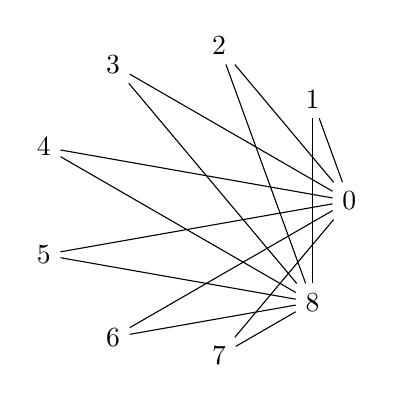
\begin{tikzpicture}
      \draw
        (0.0:2) node (0){0}
        (40.0:2) node (1){1}
        (80.0:2) node (2){2}
        (120.0:2) node (3){3}
        (160.0:2) node (4){4}
        (200.0:2) node (5){5}
        (240.0:2) node (6){6}
        (280.0:2) node (7){7}
        (320.0:2) node (8){8};
      \begin{scope}[-]
        \draw (0) to (1);
        \draw (0) to (2);
        \draw (0) to (3);
        \draw (0) to (4);
        \draw (0) to (5);
        \draw (0) to (6);
        \draw (0) to (7);
        \draw (1) to (8);
        \draw (2) to (8);
        \draw (3) to (8);
        \draw (4) to (8);
        \draw (5) to (8);
        \draw (6) to (8);
        \draw (7) to (8);
      \end{scope}
    \end{tikzpicture}
\end{figure}
\begin{itemize}
\item signature: 111111100000001000001000010001001011
\item g: Graph with 9 nodes and 14 edges
\item order: 9
\item size: 14
\item max degree: 7
\item degrees: 2,2,2,2,2,2,2,7,7
\item is tree: 0
\item is bipartite: 1
\item has bridge: 0
\item is chordal: 0
\item is complete: 0
\item min cycle basis weight: 24
\item min cycle basis size: 6
\item diameter: 2
\item radius: 2
\item is eulerian: 0
\item is planar: 1
\item number of faces: 7
\item is regular: 0
\item p3: 49
\item p4: None
\item property hash: f47fe82a8417ac36fa6b0e6e9929421f701a989b934ea204b7969b084c3d219e
\end{itemize}
\newpage
\begin{figure}
  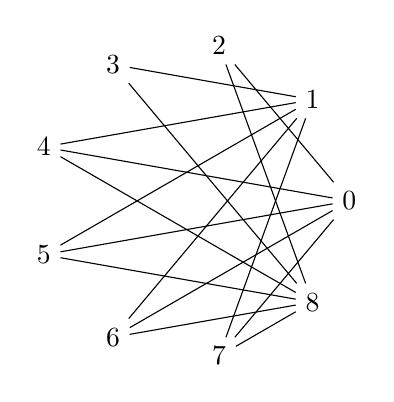
\begin{tikzpicture}
      \draw
        (0.0:2) node (0){0}
        (40.0:2) node (1){1}
        (80.0:2) node (2){2}
        (120.0:2) node (3){3}
        (160.0:2) node (4){4}
        (200.0:2) node (5){5}
        (240.0:2) node (6){6}
        (280.0:2) node (7){7}
        (320.0:2) node (8){8};
      \begin{scope}[-]
        \draw (0) to (2);
        \draw (0) to (4);
        \draw (0) to (5);
        \draw (0) to (6);
        \draw (0) to (7);
        \draw (1) to (3);
        \draw (1) to (4);
        \draw (1) to (5);
        \draw (1) to (6);
        \draw (1) to (7);
        \draw (2) to (8);
        \draw (3) to (8);
        \draw (4) to (8);
        \draw (5) to (8);
        \draw (6) to (8);
        \draw (7) to (8);
      \end{scope}
    \end{tikzpicture}
\end{figure}
\begin{itemize}
\item signature: 010111100111110000001000010001001011
\item g: Graph with 9 nodes and 16 edges
\item order: 9
\item size: 16
\item max degree: 6
\item degrees: 2,2,3,3,3,3,5,5,6
\item is tree: 0
\item is bipartite: 1
\item has bridge: 0
\item is chordal: 0
\item is complete: 0
\item min cycle basis weight: 32
\item min cycle basis size: 8
\item diameter: 3
\item radius: 2
\item is eulerian: 0
\item is planar: 0
\item number of faces: 9
\item is regular: 0
\item p3: 49
\item p4: 18
\item property hash: a33a466919ed463525090a571ad3aa42dc6fcee4e47363f6ed2e6ae11ecc59bc
\end{itemize}
\newpage
\begin{figure}
  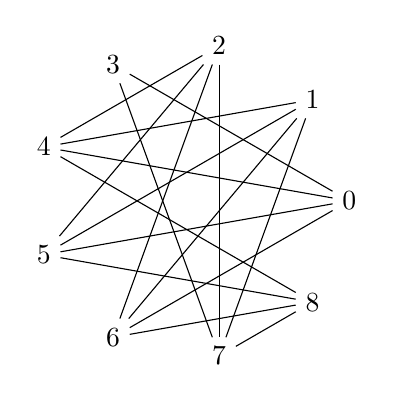
\begin{tikzpicture}
      \draw
        (0.0:2) node (0){0}
        (40.0:2) node (1){1}
        (80.0:2) node (2){2}
        (120.0:2) node (3){3}
        (160.0:2) node (4){4}
        (200.0:2) node (5){5}
        (240.0:2) node (6){6}
        (280.0:2) node (7){7}
        (320.0:2) node (8){8};
      \begin{scope}[-]
        \draw (0) to (3);
        \draw (0) to (4);
        \draw (0) to (5);
        \draw (0) to (6);
        \draw (1) to (4);
        \draw (1) to (5);
        \draw (1) to (6);
        \draw (1) to (7);
        \draw (2) to (4);
        \draw (2) to (5);
        \draw (2) to (6);
        \draw (2) to (7);
        \draw (3) to (7);
        \draw (4) to (8);
        \draw (5) to (8);
        \draw (6) to (8);
        \draw (7) to (8);
      \end{scope}
    \end{tikzpicture}
\end{figure}
\begin{itemize}
\item signature: 001111000011110011110000100001001011
\item g: Graph with 9 nodes and 17 edges
\item order: 9
\item size: 17
\item max degree: 4
\item degrees: 2,4,4,4,4,4,4,4,4
\item is tree: 0
\item is bipartite: 0
\item has bridge: 0
\item is chordal: 0
\item is complete: 0
\item min cycle basis weight: 37
\item min cycle basis size: 9
\item diameter: 2
\item radius: 2
\item is eulerian: 1
\item is planar: 0
\item number of faces: 10
\item is regular: 0
\item p3: 49
\item p4: 33
\item property hash: 86168301bc3316d04694330c8c64646120ba3bba595f6ae4ffee3df32447eb38
\end{itemize}
\newpage
\begin{figure}
  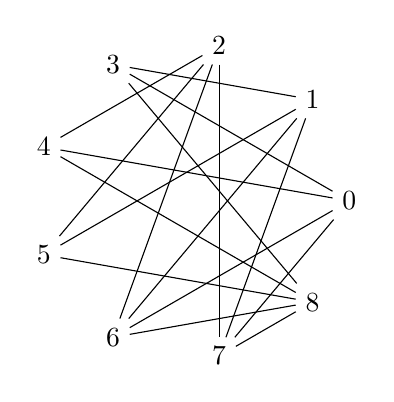
\begin{tikzpicture}
      \draw
        (0.0:2) node (0){0}
        (40.0:2) node (1){1}
        (80.0:2) node (2){2}
        (120.0:2) node (3){3}
        (160.0:2) node (4){4}
        (200.0:2) node (5){5}
        (240.0:2) node (6){6}
        (280.0:2) node (7){7}
        (320.0:2) node (8){8};
      \begin{scope}[-]
        \draw (0) to (3);
        \draw (0) to (4);
        \draw (0) to (6);
        \draw (0) to (7);
        \draw (1) to (3);
        \draw (1) to (5);
        \draw (1) to (6);
        \draw (1) to (7);
        \draw (2) to (4);
        \draw (2) to (5);
        \draw (2) to (6);
        \draw (2) to (7);
        \draw (3) to (8);
        \draw (4) to (8);
        \draw (5) to (8);
        \draw (6) to (8);
        \draw (7) to (8);
      \end{scope}
    \end{tikzpicture}
\end{figure}
\begin{itemize}
\item signature: 001101100101110011110000010001001011
\item g: Graph with 9 nodes and 17 edges
\item order: 9
\item size: 17
\item max degree: 5
\item degrees: 3,3,3,4,4,4,4,4,5
\item is tree: 0
\item is bipartite: 1
\item has bridge: 0
\item is chordal: 0
\item is complete: 0
\item min cycle basis weight: 36
\item min cycle basis size: 9
\item diameter: 3
\item radius: 2
\item is eulerian: 0
\item is planar: 0
\item number of faces: 10
\item is regular: 0
\item p3: 49
\item p4: 30
\item property hash: 5069e649b91833334c2ef995b724644aa6e2a78736eafd333c2b61ba43042fe7
\end{itemize}
\newpage
\begin{figure}
  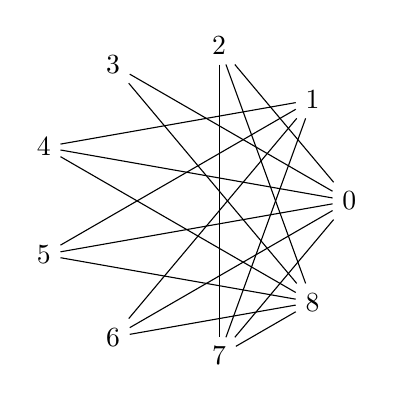
\begin{tikzpicture}
      \draw
        (0.0:2) node (0){0}
        (40.0:2) node (1){1}
        (80.0:2) node (2){2}
        (120.0:2) node (3){3}
        (160.0:2) node (4){4}
        (200.0:2) node (5){5}
        (240.0:2) node (6){6}
        (280.0:2) node (7){7}
        (320.0:2) node (8){8};
      \begin{scope}[-]
        \draw (0) to (2);
        \draw (0) to (3);
        \draw (0) to (4);
        \draw (0) to (5);
        \draw (0) to (6);
        \draw (0) to (7);
        \draw (1) to (4);
        \draw (1) to (5);
        \draw (1) to (6);
        \draw (1) to (7);
        \draw (2) to (7);
        \draw (2) to (8);
        \draw (3) to (8);
        \draw (4) to (8);
        \draw (5) to (8);
        \draw (6) to (8);
        \draw (7) to (8);
      \end{scope}
    \end{tikzpicture}
\end{figure}
\begin{itemize}
\item signature: 011111100011110000011000010001001011
\item g: Graph with 9 nodes and 17 edges
\item order: 9
\item size: 17
\item max degree: 6
\item degrees: 2,3,3,3,3,4,4,6,6
\item is tree: 0
\item is bipartite: 0
\item has bridge: 0
\item is chordal: 0
\item is complete: 0
\item min cycle basis weight: 34
\item min cycle basis size: 9
\item diameter: 3
\item radius: 2
\item is eulerian: 0
\item is planar: 0
\item number of faces: 10
\item is regular: 0
\item p3: 49
\item p4: 17
\item property hash: 026080a60130243c28554a193d07696862807b489f0ca0bf6c0617810b9d630e
\end{itemize}
\newpage
\begin{figure}
  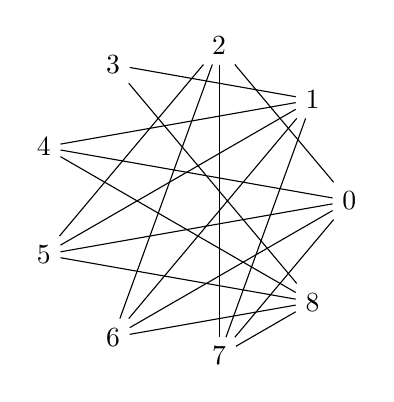
\begin{tikzpicture}
      \draw
        (0.0:2) node (0){0}
        (40.0:2) node (1){1}
        (80.0:2) node (2){2}
        (120.0:2) node (3){3}
        (160.0:2) node (4){4}
        (200.0:2) node (5){5}
        (240.0:2) node (6){6}
        (280.0:2) node (7){7}
        (320.0:2) node (8){8};
      \begin{scope}[-]
        \draw (0) to (2);
        \draw (0) to (4);
        \draw (0) to (5);
        \draw (0) to (6);
        \draw (0) to (7);
        \draw (1) to (3);
        \draw (1) to (4);
        \draw (1) to (5);
        \draw (1) to (6);
        \draw (1) to (7);
        \draw (2) to (5);
        \draw (2) to (6);
        \draw (2) to (7);
        \draw (3) to (8);
        \draw (4) to (8);
        \draw (5) to (8);
        \draw (6) to (8);
        \draw (7) to (8);
      \end{scope}
    \end{tikzpicture}
\end{figure}
\begin{itemize}
\item signature: 010111100111110001110000010001001011
\item g: Graph with 9 nodes and 18 edges
\item order: 9
\item size: 18
\item max degree: 5
\item degrees: 2,3,4,4,4,4,5,5,5
\item is tree: 0
\item is bipartite: 0
\item has bridge: 0
\item is chordal: 0
\item is complete: 0
\item min cycle basis weight: 37
\item min cycle basis size: 10
\item diameter: 3
\item radius: 2
\item is eulerian: 0
\item is planar: 0
\item number of faces: 11
\item is regular: 0
\item p3: 49
\item p4: 22
\item property hash: 7fd9cb8571cfea7a3d254bac28331f856a89a0a69505fde09e10cb15aea7d066
\end{itemize}
\newpage
\begin{figure}
  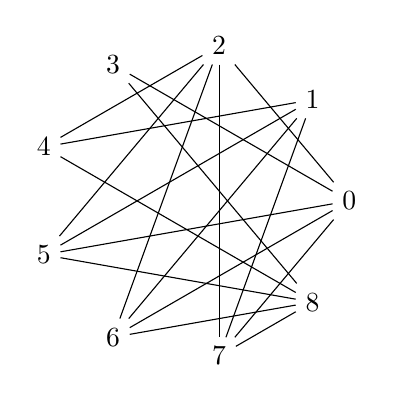
\begin{tikzpicture}
      \draw
        (0.0:2) node (0){0}
        (40.0:2) node (1){1}
        (80.0:2) node (2){2}
        (120.0:2) node (3){3}
        (160.0:2) node (4){4}
        (200.0:2) node (5){5}
        (240.0:2) node (6){6}
        (280.0:2) node (7){7}
        (320.0:2) node (8){8};
      \begin{scope}[-]
        \draw (0) to (2);
        \draw (0) to (3);
        \draw (0) to (5);
        \draw (0) to (6);
        \draw (0) to (7);
        \draw (1) to (4);
        \draw (1) to (5);
        \draw (1) to (6);
        \draw (1) to (7);
        \draw (2) to (4);
        \draw (2) to (5);
        \draw (2) to (6);
        \draw (2) to (7);
        \draw (3) to (8);
        \draw (4) to (8);
        \draw (5) to (8);
        \draw (6) to (8);
        \draw (7) to (8);
      \end{scope}
    \end{tikzpicture}
\end{figure}
\begin{itemize}
\item signature: 011011100011110011110000010001001011
\item g: Graph with 9 nodes and 18 edges
\item order: 9
\item size: 18
\item max degree: 5
\item degrees: 2,3,4,4,4,4,5,5,5
\item is tree: 0
\item is bipartite: 0
\item has bridge: 0
\item is chordal: 0
\item is complete: 0
\item min cycle basis weight: 37
\item min cycle basis size: 10
\item diameter: 3
\item radius: 2
\item is eulerian: 0
\item is planar: 0
\item number of faces: 11
\item is regular: 0
\item p3: 49
\item p4: 22
\item property hash: 7fd9cb8571cfea7a3d254bac28331f856a89a0a69505fde09e10cb15aea7d066
\end{itemize}
\newpage
\begin{figure}
  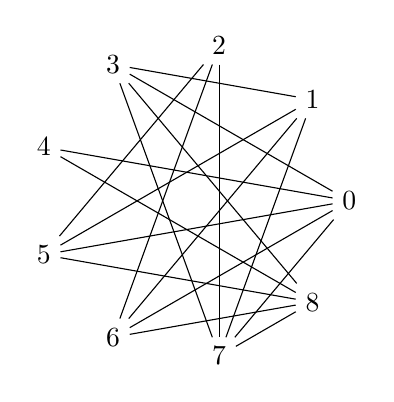
\begin{tikzpicture}
      \draw
        (0.0:2) node (0){0}
        (40.0:2) node (1){1}
        (80.0:2) node (2){2}
        (120.0:2) node (3){3}
        (160.0:2) node (4){4}
        (200.0:2) node (5){5}
        (240.0:2) node (6){6}
        (280.0:2) node (7){7}
        (320.0:2) node (8){8};
      \begin{scope}[-]
        \draw (0) to (3);
        \draw (0) to (4);
        \draw (0) to (5);
        \draw (0) to (6);
        \draw (0) to (7);
        \draw (1) to (3);
        \draw (1) to (5);
        \draw (1) to (6);
        \draw (1) to (7);
        \draw (2) to (5);
        \draw (2) to (6);
        \draw (2) to (7);
        \draw (3) to (7);
        \draw (3) to (8);
        \draw (4) to (8);
        \draw (5) to (8);
        \draw (6) to (8);
        \draw (7) to (8);
      \end{scope}
    \end{tikzpicture}
\end{figure}
\begin{itemize}
\item signature: 001111100101110001110000110001001011
\item g: Graph with 9 nodes and 18 edges
\item order: 9
\item size: 18
\item max degree: 5
\item degrees: 2,3,4,4,4,4,5,5,5
\item is tree: 0
\item is bipartite: 0
\item has bridge: 0
\item is chordal: 0
\item is complete: 0
\item min cycle basis weight: 37
\item min cycle basis size: 10
\item diameter: 3
\item radius: 2
\item is eulerian: 0
\item is planar: 0
\item number of faces: 11
\item is regular: 0
\item p3: 49
\item p4: 22
\item property hash: 7fd9cb8571cfea7a3d254bac28331f856a89a0a69505fde09e10cb15aea7d066
\end{itemize}
\newpage
\begin{figure}
  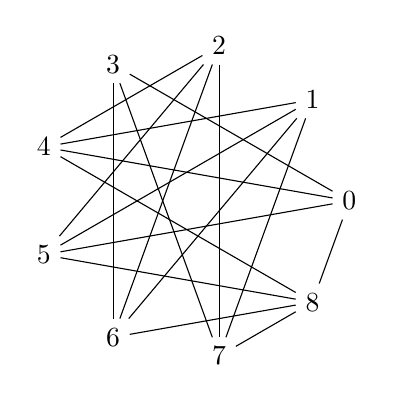
\begin{tikzpicture}
      \draw
        (0.0:2) node (0){0}
        (40.0:2) node (1){1}
        (80.0:2) node (2){2}
        (120.0:2) node (3){3}
        (160.0:2) node (4){4}
        (200.0:2) node (5){5}
        (240.0:2) node (6){6}
        (280.0:2) node (7){7}
        (320.0:2) node (8){8};
      \begin{scope}[-]
        \draw (0) to (3);
        \draw (0) to (4);
        \draw (0) to (5);
        \draw (0) to (8);
        \draw (1) to (4);
        \draw (1) to (5);
        \draw (1) to (6);
        \draw (1) to (7);
        \draw (2) to (4);
        \draw (2) to (5);
        \draw (2) to (6);
        \draw (2) to (7);
        \draw (3) to (6);
        \draw (3) to (7);
        \draw (4) to (8);
        \draw (5) to (8);
        \draw (6) to (8);
        \draw (7) to (8);
      \end{scope}
    \end{tikzpicture}
\end{figure}
\begin{itemize}
\item signature: 001110010011110011110001100001001011
\item g: Graph with 9 nodes and 18 edges
\item order: 9
\item size: 18
\item max degree: 5
\item degrees: 3,4,4,4,4,4,4,4,5
\item is tree: 0
\item is bipartite: 0
\item has bridge: 0
\item is chordal: 0
\item is complete: 0
\item min cycle basis weight: 38
\item min cycle basis size: 10
\item diameter: 2
\item radius: 2
\item is eulerian: 0
\item is planar: 0
\item number of faces: 11
\item is regular: 0
\item p3: 49
\item p4: 36
\item property hash: e3b30a0c66c1ddfc876f2aaabd1ab0a07679bf111b5057e58c60693e049420a8
\end{itemize}
\newpage
\begin{figure}
  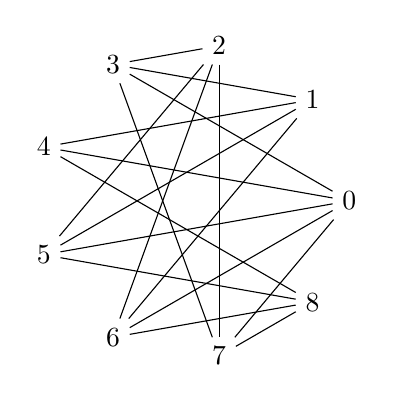
\begin{tikzpicture}
      \draw
        (0.0:2) node (0){0}
        (40.0:2) node (1){1}
        (80.0:2) node (2){2}
        (120.0:2) node (3){3}
        (160.0:2) node (4){4}
        (200.0:2) node (5){5}
        (240.0:2) node (6){6}
        (280.0:2) node (7){7}
        (320.0:2) node (8){8};
      \begin{scope}[-]
        \draw (0) to (3);
        \draw (0) to (4);
        \draw (0) to (5);
        \draw (0) to (6);
        \draw (0) to (7);
        \draw (1) to (3);
        \draw (1) to (4);
        \draw (1) to (5);
        \draw (1) to (6);
        \draw (2) to (3);
        \draw (2) to (5);
        \draw (2) to (6);
        \draw (2) to (7);
        \draw (3) to (7);
        \draw (4) to (8);
        \draw (5) to (8);
        \draw (6) to (8);
        \draw (7) to (8);
      \end{scope}
    \end{tikzpicture}
\end{figure}
\begin{itemize}
\item signature: 001111100111100101110000100001001011
\item g: Graph with 9 nodes and 18 edges
\item order: 9
\item size: 18
\item max degree: 5
\item degrees: 3,4,4,4,4,4,4,4,5
\item is tree: 0
\item is bipartite: 0
\item has bridge: 0
\item is chordal: 0
\item is complete: 0
\item min cycle basis weight: 38
\item min cycle basis size: 10
\item diameter: 3
\item radius: 2
\item is eulerian: 0
\item is planar: 0
\item number of faces: 11
\item is regular: 0
\item p3: 49
\item p4: 33
\item property hash: 0f0de7929e7f1602ff68b9ec42c52737c7fa8df34b9391a348b957adaabd1b07
\end{itemize}
\newpage
\begin{figure}
  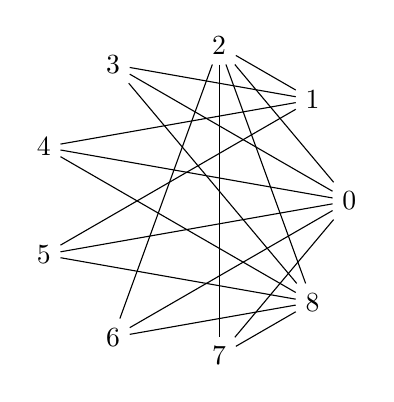
\begin{tikzpicture}
      \draw
        (0.0:2) node (0){0}
        (40.0:2) node (1){1}
        (80.0:2) node (2){2}
        (120.0:2) node (3){3}
        (160.0:2) node (4){4}
        (200.0:2) node (5){5}
        (240.0:2) node (6){6}
        (280.0:2) node (7){7}
        (320.0:2) node (8){8};
      \begin{scope}[-]
        \draw (0) to (2);
        \draw (0) to (3);
        \draw (0) to (4);
        \draw (0) to (5);
        \draw (0) to (6);
        \draw (0) to (7);
        \draw (1) to (2);
        \draw (1) to (3);
        \draw (1) to (4);
        \draw (1) to (5);
        \draw (2) to (6);
        \draw (2) to (7);
        \draw (2) to (8);
        \draw (3) to (8);
        \draw (4) to (8);
        \draw (5) to (8);
        \draw (6) to (8);
        \draw (7) to (8);
      \end{scope}
    \end{tikzpicture}
\end{figure}
\begin{itemize}
\item signature: 011111101111000000111000010001001011
\item g: Graph with 9 nodes and 18 edges
\item order: 9
\item size: 18
\item max degree: 6
\item degrees: 3,3,3,3,3,4,5,6,6
\item is tree: 0
\item is bipartite: 0
\item has bridge: 0
\item is chordal: 0
\item is complete: 0
\item min cycle basis weight: 36
\item min cycle basis size: 10
\item diameter: 2
\item radius: 2
\item is eulerian: 0
\item is planar: 0
\item number of faces: 11
\item is regular: 0
\item p3: 49
\item p4: None
\item property hash: b313c95613ceddbf7b62f63105a5ff7a181979d8206c95329ccfc6a4d94ea91d
\end{itemize}
\newpage
\begin{figure}
  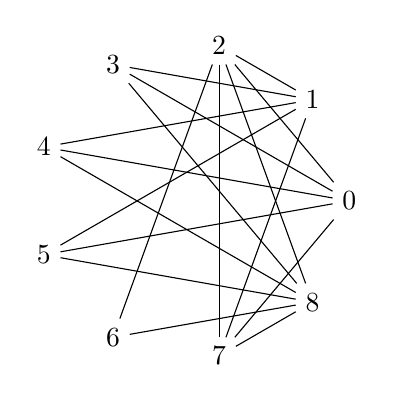
\begin{tikzpicture}
      \draw
        (0.0:2) node (0){0}
        (40.0:2) node (1){1}
        (80.0:2) node (2){2}
        (120.0:2) node (3){3}
        (160.0:2) node (4){4}
        (200.0:2) node (5){5}
        (240.0:2) node (6){6}
        (280.0:2) node (7){7}
        (320.0:2) node (8){8};
      \begin{scope}[-]
        \draw (0) to (2);
        \draw (0) to (3);
        \draw (0) to (4);
        \draw (0) to (5);
        \draw (0) to (7);
        \draw (1) to (2);
        \draw (1) to (3);
        \draw (1) to (4);
        \draw (1) to (5);
        \draw (1) to (7);
        \draw (2) to (6);
        \draw (2) to (7);
        \draw (2) to (8);
        \draw (3) to (8);
        \draw (4) to (8);
        \draw (5) to (8);
        \draw (6) to (8);
        \draw (7) to (8);
      \end{scope}
    \end{tikzpicture}
\end{figure}
\begin{itemize}
\item signature: 011110101111010000111000010001001011
\item g: Graph with 9 nodes and 18 edges
\item order: 9
\item size: 18
\item max degree: 6
\item degrees: 2,3,3,3,4,5,5,5,6
\item is tree: 0
\item is bipartite: 0
\item has bridge: 0
\item is chordal: 0
\item is complete: 0
\item min cycle basis weight: 36
\item min cycle basis size: 10
\item diameter: 2
\item radius: 2
\item is eulerian: 0
\item is planar: 0
\item number of faces: 11
\item is regular: 0
\item p3: 49
\item p4: None
\item property hash: 779028b22d4701057f1822728b53b9665ef8b5c732421927e15f88c5bd4a9f93
\end{itemize}
\newpage
\begin{figure}
  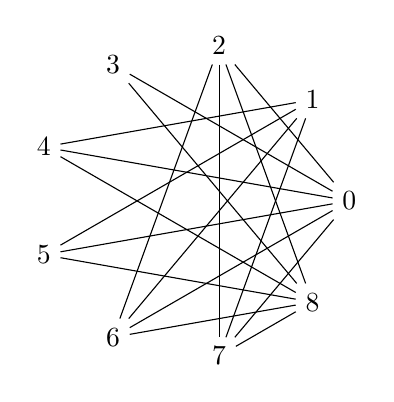
\begin{tikzpicture}
      \draw
        (0.0:2) node (0){0}
        (40.0:2) node (1){1}
        (80.0:2) node (2){2}
        (120.0:2) node (3){3}
        (160.0:2) node (4){4}
        (200.0:2) node (5){5}
        (240.0:2) node (6){6}
        (280.0:2) node (7){7}
        (320.0:2) node (8){8};
      \begin{scope}[-]
        \draw (0) to (2);
        \draw (0) to (3);
        \draw (0) to (4);
        \draw (0) to (5);
        \draw (0) to (6);
        \draw (0) to (7);
        \draw (1) to (4);
        \draw (1) to (5);
        \draw (1) to (6);
        \draw (1) to (7);
        \draw (2) to (6);
        \draw (2) to (7);
        \draw (2) to (8);
        \draw (3) to (8);
        \draw (4) to (8);
        \draw (5) to (8);
        \draw (6) to (8);
        \draw (7) to (8);
      \end{scope}
    \end{tikzpicture}
\end{figure}
\begin{itemize}
\item signature: 011111100011110000111000010001001011
\item g: Graph with 9 nodes and 18 edges
\item order: 9
\item size: 18
\item max degree: 6
\item degrees: 2,3,3,4,4,4,4,6,6
\item is tree: 0
\item is bipartite: 0
\item has bridge: 0
\item is chordal: 0
\item is complete: 0
\item min cycle basis weight: 36
\item min cycle basis size: 10
\item diameter: 3
\item radius: 2
\item is eulerian: 0
\item is planar: 0
\item number of faces: 11
\item is regular: 0
\item p3: 49
\item p4: 16
\item property hash: f538d118ceca5969b46976a6beecd802c97ff683d9a91c27992757939ae57666
\end{itemize}
\newpage
\begin{figure}
  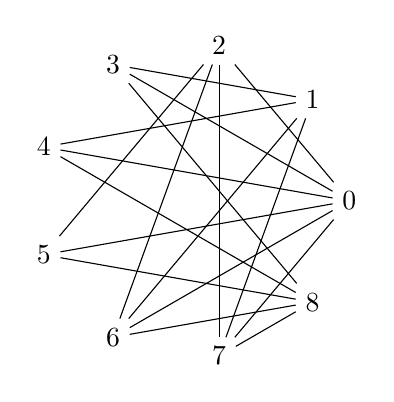
\begin{tikzpicture}
      \draw
        (0.0:2) node (0){0}
        (40.0:2) node (1){1}
        (80.0:2) node (2){2}
        (120.0:2) node (3){3}
        (160.0:2) node (4){4}
        (200.0:2) node (5){5}
        (240.0:2) node (6){6}
        (280.0:2) node (7){7}
        (320.0:2) node (8){8};
      \begin{scope}[-]
        \draw (0) to (2);
        \draw (0) to (3);
        \draw (0) to (4);
        \draw (0) to (5);
        \draw (0) to (6);
        \draw (0) to (7);
        \draw (1) to (3);
        \draw (1) to (4);
        \draw (1) to (6);
        \draw (1) to (7);
        \draw (2) to (5);
        \draw (2) to (6);
        \draw (2) to (7);
        \draw (3) to (8);
        \draw (4) to (8);
        \draw (5) to (8);
        \draw (6) to (8);
        \draw (7) to (8);
      \end{scope}
    \end{tikzpicture}
\end{figure}
\begin{itemize}
\item signature: 011111100110110001110000010001001011
\item g: Graph with 9 nodes and 18 edges
\item order: 9
\item size: 18
\item max degree: 6
\item degrees: 3,3,3,4,4,4,4,5,6
\item is tree: 0
\item is bipartite: 0
\item has bridge: 0
\item is chordal: 0
\item is complete: 0
\item min cycle basis weight: 37
\item min cycle basis size: 10
\item diameter: 3
\item radius: 2
\item is eulerian: 0
\item is planar: 0
\item number of faces: 11
\item is regular: 0
\item p3: 49
\item p4: 24
\item property hash: e28744705935a372c54e86e78880b536b883d16ae5546c5de7b44ac0da4f3496
\end{itemize}
\newpage
\begin{figure}
  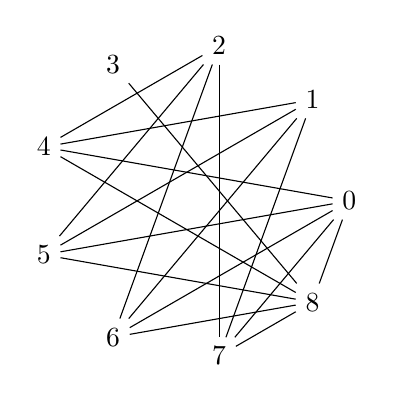
\begin{tikzpicture}
      \draw
        (0.0:2) node (0){0}
        (40.0:2) node (1){1}
        (80.0:2) node (2){2}
        (120.0:2) node (3){3}
        (160.0:2) node (4){4}
        (200.0:2) node (5){5}
        (240.0:2) node (6){6}
        (280.0:2) node (7){7}
        (320.0:2) node (8){8};
      \begin{scope}[-]
        \draw (0) to (4);
        \draw (0) to (5);
        \draw (0) to (6);
        \draw (0) to (7);
        \draw (0) to (8);
        \draw (1) to (4);
        \draw (1) to (5);
        \draw (1) to (6);
        \draw (1) to (7);
        \draw (2) to (4);
        \draw (2) to (5);
        \draw (2) to (6);
        \draw (2) to (7);
        \draw (3) to (8);
        \draw (4) to (8);
        \draw (5) to (8);
        \draw (6) to (8);
        \draw (7) to (8);
      \end{scope}
    \end{tikzpicture}
\end{figure}
\begin{itemize}
\item signature: 000111110011110011110000010001001011
\item g: Graph with 9 nodes and 18 edges
\item order: 9
\item size: 18
\item max degree: 6
\item degrees: 1,4,4,4,4,4,4,5,6
\item is tree: 0
\item is bipartite: 0
\item has bridge: 1
\item is chordal: 0
\item is complete: 0
\item min cycle basis weight: 36
\item min cycle basis size: 10
\item diameter: 3
\item radius: 2
\item is eulerian: 0
\item is planar: 0
\item number of faces: 11
\item is regular: 0
\item p3: 49
\item p4: None
\item property hash: fb537e6c5a91275734289a18da6c6fd7d07bf3968530f345b0fca48c1a089c6d
\end{itemize}
\newpage
\begin{figure}
  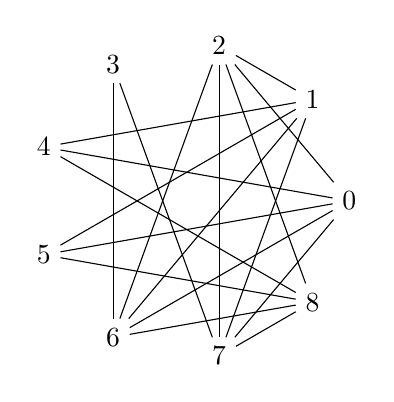
\begin{tikzpicture}
      \draw
        (0.0:2) node (0){0}
        (40.0:2) node (1){1}
        (80.0:2) node (2){2}
        (120.0:2) node (3){3}
        (160.0:2) node (4){4}
        (200.0:2) node (5){5}
        (240.0:2) node (6){6}
        (280.0:2) node (7){7}
        (320.0:2) node (8){8};
      \begin{scope}[-]
        \draw (0) to (2);
        \draw (0) to (4);
        \draw (0) to (5);
        \draw (0) to (6);
        \draw (0) to (7);
        \draw (1) to (2);
        \draw (1) to (4);
        \draw (1) to (5);
        \draw (1) to (6);
        \draw (1) to (7);
        \draw (2) to (6);
        \draw (2) to (7);
        \draw (2) to (8);
        \draw (3) to (6);
        \draw (3) to (7);
        \draw (4) to (8);
        \draw (5) to (8);
        \draw (6) to (8);
        \draw (7) to (8);
      \end{scope}
    \end{tikzpicture}
\end{figure}
\begin{itemize}
\item signature: 010111101011110000111001100001001011
\item g: Graph with 9 nodes and 19 edges
\item order: 9
\item size: 19
\item max degree: 5
\item degrees: 2,3,3,5,5,5,5,5,5
\item is tree: 0
\item is bipartite: 0
\item has bridge: 0
\item is chordal: 0
\item is complete: 0
\item min cycle basis weight: 38
\item min cycle basis size: 11
\item diameter: 3
\item radius: 2
\item is eulerian: 0
\item is planar: 0
\item number of faces: 12
\item is regular: 0
\item p3: 49
\item p4: None
\item property hash: d29ba5ee3540cafdd1eccb423af0092386d507a090d4b40a80573aba77f6ba4b
\end{itemize}
\newpage
\begin{figure}
  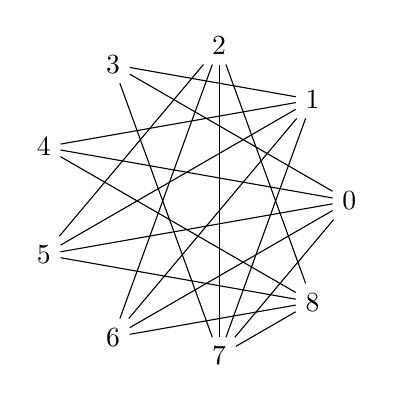
\begin{tikzpicture}
      \draw
        (0.0:2) node (0){0}
        (40.0:2) node (1){1}
        (80.0:2) node (2){2}
        (120.0:2) node (3){3}
        (160.0:2) node (4){4}
        (200.0:2) node (5){5}
        (240.0:2) node (6){6}
        (280.0:2) node (7){7}
        (320.0:2) node (8){8};
      \begin{scope}[-]
        \draw (0) to (3);
        \draw (0) to (4);
        \draw (0) to (5);
        \draw (0) to (6);
        \draw (0) to (7);
        \draw (1) to (3);
        \draw (1) to (4);
        \draw (1) to (5);
        \draw (1) to (6);
        \draw (1) to (7);
        \draw (2) to (5);
        \draw (2) to (6);
        \draw (2) to (7);
        \draw (2) to (8);
        \draw (3) to (7);
        \draw (4) to (8);
        \draw (5) to (8);
        \draw (6) to (8);
        \draw (7) to (8);
      \end{scope}
    \end{tikzpicture}
\end{figure}
\begin{itemize}
\item signature: 001111100111110001111000100001001011
\item g: Graph with 9 nodes and 19 edges
\item order: 9
\item size: 19
\item max degree: 5
\item degrees: 3,3,4,4,4,5,5,5,5
\item is tree: 0
\item is bipartite: 0
\item has bridge: 0
\item is chordal: 0
\item is complete: 0
\item min cycle basis weight: 39
\item min cycle basis size: 11
\item diameter: 2
\item radius: 2
\item is eulerian: 0
\item is planar: 0
\item number of faces: 12
\item is regular: 0
\item p3: 49
\item p4: 23
\item property hash: 8ef0e54b9717cf96791df08c89b5f957e575255e65e577c0c86162e7c666664c
\end{itemize}
\newpage
\begin{figure}
  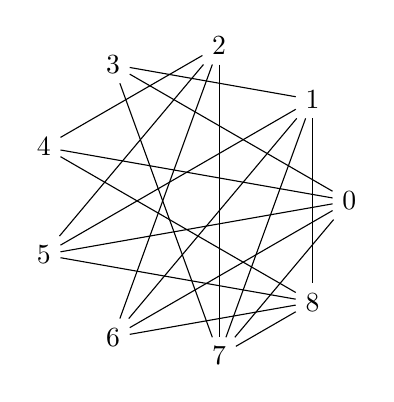
\begin{tikzpicture}
      \draw
        (0.0:2) node (0){0}
        (40.0:2) node (1){1}
        (80.0:2) node (2){2}
        (120.0:2) node (3){3}
        (160.0:2) node (4){4}
        (200.0:2) node (5){5}
        (240.0:2) node (6){6}
        (280.0:2) node (7){7}
        (320.0:2) node (8){8};
      \begin{scope}[-]
        \draw (0) to (3);
        \draw (0) to (4);
        \draw (0) to (5);
        \draw (0) to (6);
        \draw (0) to (7);
        \draw (1) to (3);
        \draw (1) to (5);
        \draw (1) to (6);
        \draw (1) to (7);
        \draw (1) to (8);
        \draw (2) to (4);
        \draw (2) to (5);
        \draw (2) to (6);
        \draw (2) to (7);
        \draw (3) to (7);
        \draw (4) to (8);
        \draw (5) to (8);
        \draw (6) to (8);
        \draw (7) to (8);
      \end{scope}
    \end{tikzpicture}
\end{figure}
\begin{itemize}
\item signature: 001111100101111011110000100001001011
\item g: Graph with 9 nodes and 19 edges
\item order: 9
\item size: 19
\item max degree: 5
\item degrees: 3,3,4,4,4,5,5,5,5
\item is tree: 0
\item is bipartite: 0
\item has bridge: 0
\item is chordal: 0
\item is complete: 0
\item min cycle basis weight: 39
\item min cycle basis size: 11
\item diameter: 2
\item radius: 2
\item is eulerian: 0
\item is planar: 0
\item number of faces: 12
\item is regular: 0
\item p3: 49
\item p4: 25
\item property hash: fa6c706c401c3033679e853699984d736f1b06cf828d3b4488925bd92b65f072
\end{itemize}
\newpage
\begin{figure}
  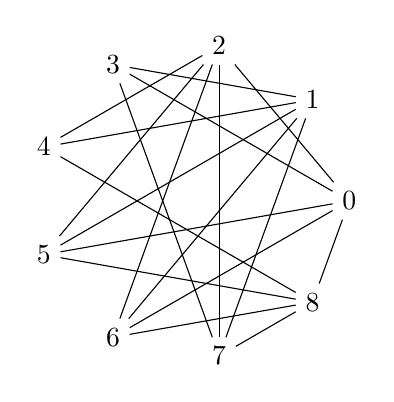
\begin{tikzpicture}
      \draw
        (0.0:2) node (0){0}
        (40.0:2) node (1){1}
        (80.0:2) node (2){2}
        (120.0:2) node (3){3}
        (160.0:2) node (4){4}
        (200.0:2) node (5){5}
        (240.0:2) node (6){6}
        (280.0:2) node (7){7}
        (320.0:2) node (8){8};
      \begin{scope}[-]
        \draw (0) to (2);
        \draw (0) to (3);
        \draw (0) to (5);
        \draw (0) to (6);
        \draw (0) to (8);
        \draw (1) to (3);
        \draw (1) to (4);
        \draw (1) to (5);
        \draw (1) to (6);
        \draw (1) to (7);
        \draw (2) to (4);
        \draw (2) to (5);
        \draw (2) to (6);
        \draw (2) to (7);
        \draw (3) to (7);
        \draw (4) to (8);
        \draw (5) to (8);
        \draw (6) to (8);
        \draw (7) to (8);
      \end{scope}
    \end{tikzpicture}
\end{figure}
\begin{itemize}
\item signature: 011011010111110011110000100001001011
\item g: Graph with 9 nodes and 19 edges
\item order: 9
\item size: 19
\item max degree: 5
\item degrees: 3,3,4,4,4,5,5,5,5
\item is tree: 0
\item is bipartite: 0
\item has bridge: 0
\item is chordal: 0
\item is complete: 0
\item min cycle basis weight: 39
\item min cycle basis size: 11
\item diameter: 2
\item radius: 2
\item is eulerian: 0
\item is planar: 0
\item number of faces: 12
\item is regular: 0
\item p3: 49
\item p4: 27
\item property hash: 1cc6d2a1b8c375762388f5520330e5ed7499746c222000789e770ad84350bfba
\end{itemize}
\newpage
\begin{figure}
  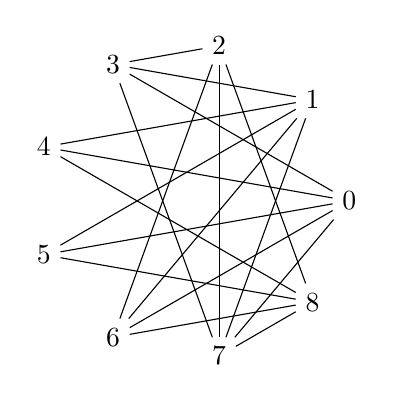
\begin{tikzpicture}
      \draw
        (0.0:2) node (0){0}
        (40.0:2) node (1){1}
        (80.0:2) node (2){2}
        (120.0:2) node (3){3}
        (160.0:2) node (4){4}
        (200.0:2) node (5){5}
        (240.0:2) node (6){6}
        (280.0:2) node (7){7}
        (320.0:2) node (8){8};
      \begin{scope}[-]
        \draw (0) to (3);
        \draw (0) to (4);
        \draw (0) to (5);
        \draw (0) to (6);
        \draw (0) to (7);
        \draw (1) to (3);
        \draw (1) to (4);
        \draw (1) to (5);
        \draw (1) to (6);
        \draw (1) to (7);
        \draw (2) to (3);
        \draw (2) to (6);
        \draw (2) to (7);
        \draw (2) to (8);
        \draw (3) to (7);
        \draw (4) to (8);
        \draw (5) to (8);
        \draw (6) to (8);
        \draw (7) to (8);
      \end{scope}
    \end{tikzpicture}
\end{figure}
\begin{itemize}
\item signature: 001111100111110100111000100001001011
\item g: Graph with 9 nodes and 19 edges
\item order: 9
\item size: 19
\item max degree: 5
\item degrees: 3,3,4,4,4,5,5,5,5
\item is tree: 0
\item is bipartite: 0
\item has bridge: 0
\item is chordal: 0
\item is complete: 0
\item min cycle basis weight: 39
\item min cycle basis size: 11
\item diameter: 2
\item radius: 2
\item is eulerian: 0
\item is planar: 0
\item number of faces: 12
\item is regular: 0
\item p3: 49
\item p4: 29
\item property hash: 43097673c4f11f3e802de92794681cfb72039c50b279a99dc30ad9b84a10db54
\end{itemize}
\newpage
\begin{figure}
  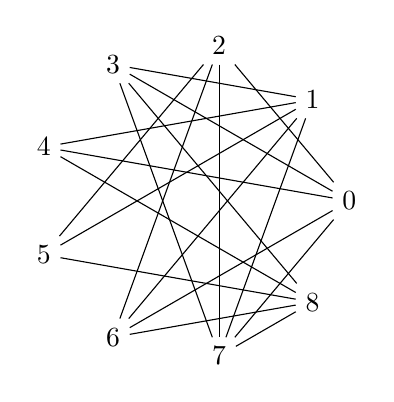
\begin{tikzpicture}
      \draw
        (0.0:2) node (0){0}
        (40.0:2) node (1){1}
        (80.0:2) node (2){2}
        (120.0:2) node (3){3}
        (160.0:2) node (4){4}
        (200.0:2) node (5){5}
        (240.0:2) node (6){6}
        (280.0:2) node (7){7}
        (320.0:2) node (8){8};
      \begin{scope}[-]
        \draw (0) to (2);
        \draw (0) to (3);
        \draw (0) to (4);
        \draw (0) to (6);
        \draw (0) to (7);
        \draw (1) to (3);
        \draw (1) to (4);
        \draw (1) to (5);
        \draw (1) to (6);
        \draw (1) to (7);
        \draw (2) to (5);
        \draw (2) to (6);
        \draw (2) to (7);
        \draw (3) to (7);
        \draw (3) to (8);
        \draw (4) to (8);
        \draw (5) to (8);
        \draw (6) to (8);
        \draw (7) to (8);
      \end{scope}
    \end{tikzpicture}
\end{figure}
\begin{itemize}
\item signature: 011101100111110001110000110001001011
\item g: Graph with 9 nodes and 19 edges
\item order: 9
\item size: 19
\item max degree: 5
\item degrees: 3,3,4,4,4,5,5,5,5
\item is tree: 0
\item is bipartite: 0
\item has bridge: 0
\item is chordal: 0
\item is complete: 0
\item min cycle basis weight: 39
\item min cycle basis size: 11
\item diameter: 2
\item radius: 2
\item is eulerian: 0
\item is planar: 0
\item number of faces: 12
\item is regular: 0
\item p3: 49
\item p4: 28
\item property hash: db7d22cfcf4dfdf1501e17a45921575445e4eda96996dce090431a8d4fa60f85
\end{itemize}
\newpage
\begin{figure}
  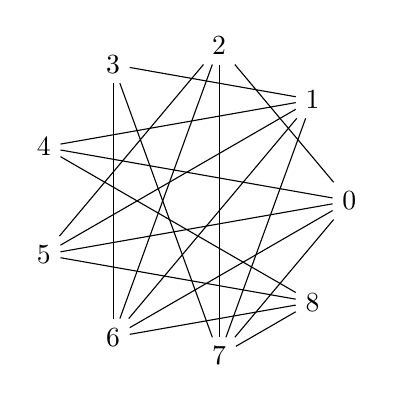
\begin{tikzpicture}
      \draw
        (0.0:2) node (0){0}
        (40.0:2) node (1){1}
        (80.0:2) node (2){2}
        (120.0:2) node (3){3}
        (160.0:2) node (4){4}
        (200.0:2) node (5){5}
        (240.0:2) node (6){6}
        (280.0:2) node (7){7}
        (320.0:2) node (8){8};
      \begin{scope}[-]
        \draw (0) to (2);
        \draw (0) to (4);
        \draw (0) to (5);
        \draw (0) to (6);
        \draw (0) to (7);
        \draw (1) to (3);
        \draw (1) to (4);
        \draw (1) to (5);
        \draw (1) to (6);
        \draw (1) to (7);
        \draw (2) to (5);
        \draw (2) to (6);
        \draw (2) to (7);
        \draw (3) to (6);
        \draw (3) to (7);
        \draw (4) to (8);
        \draw (5) to (8);
        \draw (6) to (8);
        \draw (7) to (8);
      \end{scope}
    \end{tikzpicture}
\end{figure}
\begin{itemize}
\item signature: 010111100111110001110001100001001011
\item g: Graph with 9 nodes and 19 edges
\item order: 9
\item size: 19
\item max degree: 5
\item degrees: 3,3,4,4,4,5,5,5,5
\item is tree: 0
\item is bipartite: 0
\item has bridge: 0
\item is chordal: 0
\item is complete: 0
\item min cycle basis weight: 39
\item min cycle basis size: 11
\item diameter: 2
\item radius: 2
\item is eulerian: 0
\item is planar: 0
\item number of faces: 12
\item is regular: 0
\item p3: 49
\item p4: 23
\item property hash: 8ef0e54b9717cf96791df08c89b5f957e575255e65e577c0c86162e7c666664c
\end{itemize}
\newpage
\begin{figure}
  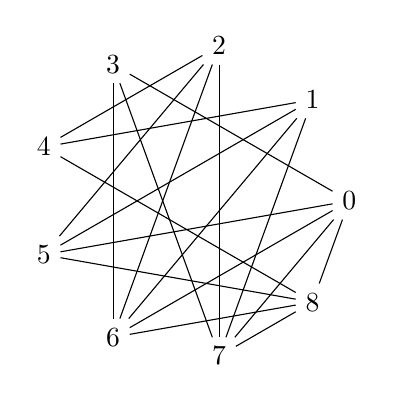
\begin{tikzpicture}
      \draw
        (0.0:2) node (0){0}
        (40.0:2) node (1){1}
        (80.0:2) node (2){2}
        (120.0:2) node (3){3}
        (160.0:2) node (4){4}
        (200.0:2) node (5){5}
        (240.0:2) node (6){6}
        (280.0:2) node (7){7}
        (320.0:2) node (8){8};
      \begin{scope}[-]
        \draw (0) to (3);
        \draw (0) to (5);
        \draw (0) to (6);
        \draw (0) to (7);
        \draw (0) to (8);
        \draw (1) to (4);
        \draw (1) to (5);
        \draw (1) to (6);
        \draw (1) to (7);
        \draw (2) to (4);
        \draw (2) to (5);
        \draw (2) to (6);
        \draw (2) to (7);
        \draw (3) to (6);
        \draw (3) to (7);
        \draw (4) to (8);
        \draw (5) to (8);
        \draw (6) to (8);
        \draw (7) to (8);
      \end{scope}
    \end{tikzpicture}
\end{figure}
\begin{itemize}
\item signature: 001011110011110011110001100001001011
\item g: Graph with 9 nodes and 19 edges
\item order: 9
\item size: 19
\item max degree: 5
\item degrees: 3,3,4,4,4,5,5,5,5
\item is tree: 0
\item is bipartite: 0
\item has bridge: 0
\item is chordal: 0
\item is complete: 0
\item min cycle basis weight: 39
\item min cycle basis size: 11
\item diameter: 3
\item radius: 2
\item is eulerian: 0
\item is planar: 0
\item number of faces: 12
\item is regular: 0
\item p3: 49
\item p4: 23
\item property hash: d0edab54f88065dd439d6fb073bec4695625f82d3abfb3962d710bb7e7621ddf
\end{itemize}
\newpage
\begin{figure}
  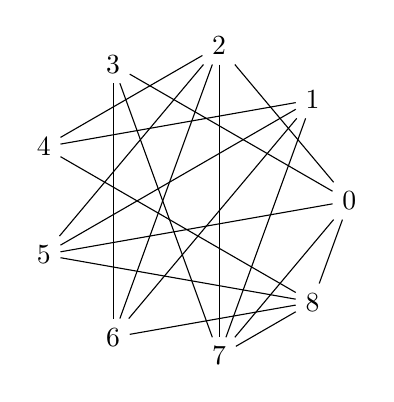
\begin{tikzpicture}
      \draw
        (0.0:2) node (0){0}
        (40.0:2) node (1){1}
        (80.0:2) node (2){2}
        (120.0:2) node (3){3}
        (160.0:2) node (4){4}
        (200.0:2) node (5){5}
        (240.0:2) node (6){6}
        (280.0:2) node (7){7}
        (320.0:2) node (8){8};
      \begin{scope}[-]
        \draw (0) to (2);
        \draw (0) to (3);
        \draw (0) to (5);
        \draw (0) to (7);
        \draw (0) to (8);
        \draw (1) to (4);
        \draw (1) to (5);
        \draw (1) to (6);
        \draw (1) to (7);
        \draw (2) to (4);
        \draw (2) to (5);
        \draw (2) to (6);
        \draw (2) to (7);
        \draw (3) to (6);
        \draw (3) to (7);
        \draw (4) to (8);
        \draw (5) to (8);
        \draw (6) to (8);
        \draw (7) to (8);
      \end{scope}
    \end{tikzpicture}
\end{figure}
\begin{itemize}
\item signature: 011010110011110011110001100001001011
\item g: Graph with 9 nodes and 19 edges
\item order: 9
\item size: 19
\item max degree: 5
\item degrees: 3,3,4,4,4,5,5,5,5
\item is tree: 0
\item is bipartite: 0
\item has bridge: 0
\item is chordal: 0
\item is complete: 0
\item min cycle basis weight: 39
\item min cycle basis size: 11
\item diameter: 3
\item radius: 2
\item is eulerian: 0
\item is planar: 0
\item number of faces: 12
\item is regular: 0
\item p3: 49
\item p4: 25
\item property hash: 9badf88476cbb35af7f7708b29becf66e6f79886458fb17c730b318a23ab0f09
\end{itemize}
\newpage
\begin{figure}
  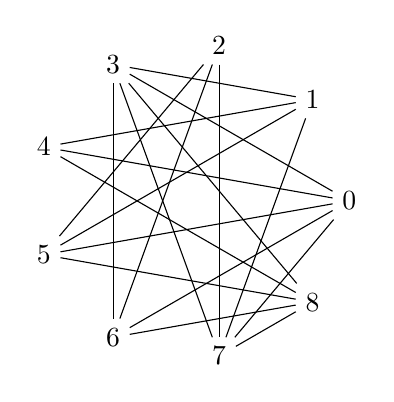
\begin{tikzpicture}
      \draw
        (0.0:2) node (0){0}
        (40.0:2) node (1){1}
        (80.0:2) node (2){2}
        (120.0:2) node (3){3}
        (160.0:2) node (4){4}
        (200.0:2) node (5){5}
        (240.0:2) node (6){6}
        (280.0:2) node (7){7}
        (320.0:2) node (8){8};
      \begin{scope}[-]
        \draw (0) to (3);
        \draw (0) to (4);
        \draw (0) to (5);
        \draw (0) to (6);
        \draw (0) to (7);
        \draw (1) to (3);
        \draw (1) to (4);
        \draw (1) to (5);
        \draw (1) to (7);
        \draw (2) to (5);
        \draw (2) to (6);
        \draw (2) to (7);
        \draw (3) to (6);
        \draw (3) to (7);
        \draw (3) to (8);
        \draw (4) to (8);
        \draw (5) to (8);
        \draw (6) to (8);
        \draw (7) to (8);
      \end{scope}
    \end{tikzpicture}
\end{figure}
\begin{itemize}
\item signature: 001111100111010001110001110001001011
\item g: Graph with 9 nodes and 19 edges
\item order: 9
\item size: 19
\item max degree: 5
\item degrees: 3,3,4,4,4,5,5,5,5
\item is tree: 0
\item is bipartite: 0
\item has bridge: 0
\item is chordal: 0
\item is complete: 0
\item min cycle basis weight: 39
\item min cycle basis size: 11
\item diameter: 3
\item radius: 2
\item is eulerian: 0
\item is planar: 0
\item number of faces: 12
\item is regular: 0
\item p3: 49
\item p4: 24
\item property hash: d81a0ad87e9655693fa4f6e30a2e7a43ae67ad7c1b588764ac67e9afb58ea9a2
\end{itemize}
\newpage
\begin{figure}
  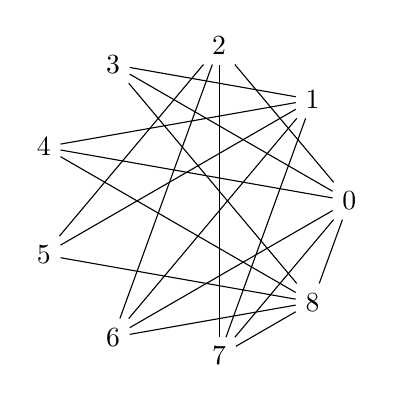
\begin{tikzpicture}
      \draw
        (0.0:2) node (0){0}
        (40.0:2) node (1){1}
        (80.0:2) node (2){2}
        (120.0:2) node (3){3}
        (160.0:2) node (4){4}
        (200.0:2) node (5){5}
        (240.0:2) node (6){6}
        (280.0:2) node (7){7}
        (320.0:2) node (8){8};
      \begin{scope}[-]
        \draw (0) to (2);
        \draw (0) to (3);
        \draw (0) to (4);
        \draw (0) to (6);
        \draw (0) to (7);
        \draw (0) to (8);
        \draw (1) to (3);
        \draw (1) to (4);
        \draw (1) to (5);
        \draw (1) to (6);
        \draw (1) to (7);
        \draw (2) to (5);
        \draw (2) to (6);
        \draw (2) to (7);
        \draw (3) to (8);
        \draw (4) to (8);
        \draw (5) to (8);
        \draw (6) to (8);
        \draw (7) to (8);
      \end{scope}
    \end{tikzpicture}
\end{figure}
\begin{itemize}
\item signature: 011101110111110001110000010001001011
\item g: Graph with 9 nodes and 19 edges
\item order: 9
\item size: 19
\item max degree: 6
\item degrees: 3,3,3,4,4,4,5,6,6
\item is tree: 0
\item is bipartite: 0
\item has bridge: 0
\item is chordal: 0
\item is complete: 0
\item min cycle basis weight: 38
\item min cycle basis size: 11
\item diameter: 2
\item radius: 2
\item is eulerian: 0
\item is planar: 0
\item number of faces: 12
\item is regular: 0
\item p3: 49
\item p4: 22
\item property hash: 7b01ce12db5d1a40e12c925652c0dd30c04ef1eced30ad7579a6da676be79da6
\end{itemize}
\newpage
\begin{figure}
  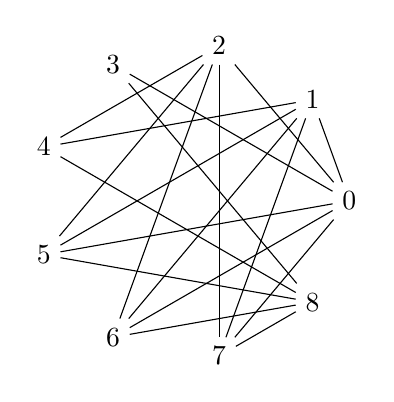
\begin{tikzpicture}
      \draw
        (0.0:2) node (0){0}
        (40.0:2) node (1){1}
        (80.0:2) node (2){2}
        (120.0:2) node (3){3}
        (160.0:2) node (4){4}
        (200.0:2) node (5){5}
        (240.0:2) node (6){6}
        (280.0:2) node (7){7}
        (320.0:2) node (8){8};
      \begin{scope}[-]
        \draw (0) to (1);
        \draw (0) to (2);
        \draw (0) to (3);
        \draw (0) to (5);
        \draw (0) to (6);
        \draw (0) to (7);
        \draw (1) to (4);
        \draw (1) to (5);
        \draw (1) to (6);
        \draw (1) to (7);
        \draw (2) to (4);
        \draw (2) to (5);
        \draw (2) to (6);
        \draw (2) to (7);
        \draw (3) to (8);
        \draw (4) to (8);
        \draw (5) to (8);
        \draw (6) to (8);
        \draw (7) to (8);
      \end{scope}
    \end{tikzpicture}
\end{figure}
\begin{itemize}
\item signature: 111011100011110011110000010001001011
\item g: Graph with 9 nodes and 19 edges
\item order: 9
\item size: 19
\item max degree: 6
\item degrees: 2,3,4,4,4,5,5,5,6
\item is tree: 0
\item is bipartite: 0
\item has bridge: 0
\item is chordal: 0
\item is complete: 0
\item min cycle basis weight: 38
\item min cycle basis size: 11
\item diameter: 2
\item radius: 2
\item is eulerian: 0
\item is planar: 0
\item number of faces: 12
\item is regular: 0
\item p3: 49
\item p4: 18
\item property hash: 85828af3e5776efa182b8bd8a016531dd0fc24a6e94aac4920fe092171b996a8
\end{itemize}
\newpage
\begin{figure}
  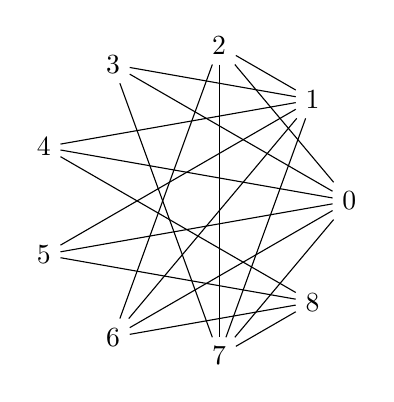
\begin{tikzpicture}
      \draw
        (0.0:2) node (0){0}
        (40.0:2) node (1){1}
        (80.0:2) node (2){2}
        (120.0:2) node (3){3}
        (160.0:2) node (4){4}
        (200.0:2) node (5){5}
        (240.0:2) node (6){6}
        (280.0:2) node (7){7}
        (320.0:2) node (8){8};
      \begin{scope}[-]
        \draw (0) to (2);
        \draw (0) to (3);
        \draw (0) to (4);
        \draw (0) to (5);
        \draw (0) to (6);
        \draw (0) to (7);
        \draw (1) to (2);
        \draw (1) to (3);
        \draw (1) to (4);
        \draw (1) to (5);
        \draw (1) to (6);
        \draw (1) to (7);
        \draw (2) to (6);
        \draw (2) to (7);
        \draw (3) to (7);
        \draw (4) to (8);
        \draw (5) to (8);
        \draw (6) to (8);
        \draw (7) to (8);
      \end{scope}
    \end{tikzpicture}
\end{figure}
\begin{itemize}
\item signature: 011111101111110000110000100001001011
\item g: Graph with 9 nodes and 19 edges
\item order: 9
\item size: 19
\item max degree: 6
\item degrees: 3,3,3,4,4,4,5,6,6
\item is tree: 0
\item is bipartite: 0
\item has bridge: 0
\item is chordal: 0
\item is complete: 0
\item min cycle basis weight: 38
\item min cycle basis size: 11
\item diameter: 2
\item radius: 2
\item is eulerian: 0
\item is planar: 0
\item number of faces: 12
\item is regular: 0
\item p3: 49
\item p4: None
\item property hash: 18ad3f2d2d0c1477cd6f93ba2df618c1d843dd700995c98c9925974b31787fd4
\end{itemize}
\newpage
\begin{figure}
  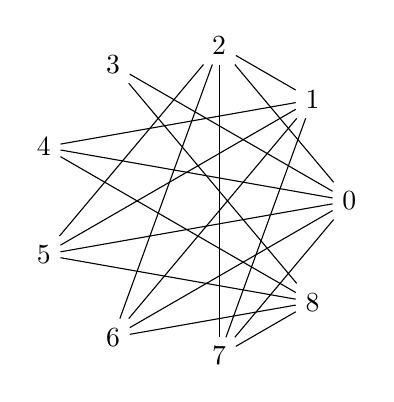
\begin{tikzpicture}
      \draw
        (0.0:2) node (0){0}
        (40.0:2) node (1){1}
        (80.0:2) node (2){2}
        (120.0:2) node (3){3}
        (160.0:2) node (4){4}
        (200.0:2) node (5){5}
        (240.0:2) node (6){6}
        (280.0:2) node (7){7}
        (320.0:2) node (8){8};
      \begin{scope}[-]
        \draw (0) to (2);
        \draw (0) to (3);
        \draw (0) to (4);
        \draw (0) to (5);
        \draw (0) to (6);
        \draw (0) to (7);
        \draw (1) to (2);
        \draw (1) to (4);
        \draw (1) to (5);
        \draw (1) to (6);
        \draw (1) to (7);
        \draw (2) to (5);
        \draw (2) to (6);
        \draw (2) to (7);
        \draw (3) to (8);
        \draw (4) to (8);
        \draw (5) to (8);
        \draw (6) to (8);
        \draw (7) to (8);
      \end{scope}
    \end{tikzpicture}
\end{figure}
\begin{itemize}
\item signature: 011111101011110001110000010001001011
\item g: Graph with 9 nodes and 19 edges
\item order: 9
\item size: 19
\item max degree: 6
\item degrees: 2,3,4,4,4,5,5,5,6
\item is tree: 0
\item is bipartite: 0
\item has bridge: 0
\item is chordal: 0
\item is complete: 0
\item min cycle basis weight: 38
\item min cycle basis size: 11
\item diameter: 3
\item radius: 2
\item is eulerian: 0
\item is planar: 0
\item number of faces: 12
\item is regular: 0
\item p3: 49
\item p4: 18
\item property hash: 83aa3a29804ff8c328b163ef4551b5357cb75199fb36be50599c99350fc8b1f2
\end{itemize}
\newpage
\begin{figure}
  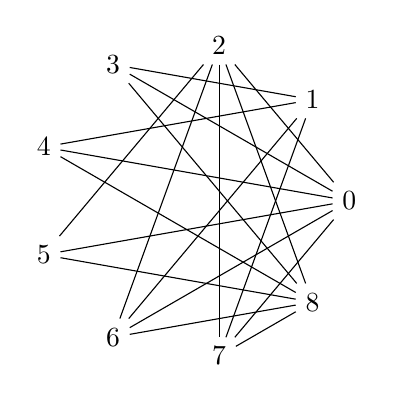
\begin{tikzpicture}
      \draw
        (0.0:2) node (0){0}
        (40.0:2) node (1){1}
        (80.0:2) node (2){2}
        (120.0:2) node (3){3}
        (160.0:2) node (4){4}
        (200.0:2) node (5){5}
        (240.0:2) node (6){6}
        (280.0:2) node (7){7}
        (320.0:2) node (8){8};
      \begin{scope}[-]
        \draw (0) to (2);
        \draw (0) to (3);
        \draw (0) to (4);
        \draw (0) to (5);
        \draw (0) to (6);
        \draw (0) to (7);
        \draw (1) to (3);
        \draw (1) to (4);
        \draw (1) to (6);
        \draw (1) to (7);
        \draw (2) to (5);
        \draw (2) to (6);
        \draw (2) to (7);
        \draw (2) to (8);
        \draw (3) to (8);
        \draw (4) to (8);
        \draw (5) to (8);
        \draw (6) to (8);
        \draw (7) to (8);
      \end{scope}
    \end{tikzpicture}
\end{figure}
\begin{itemize}
\item signature: 011111100110110001111000010001001011
\item g: Graph with 9 nodes and 19 edges
\item order: 9
\item size: 19
\item max degree: 6
\item degrees: 3,3,3,4,4,4,5,6,6
\item is tree: 0
\item is bipartite: 0
\item has bridge: 0
\item is chordal: 0
\item is complete: 0
\item min cycle basis weight: 38
\item min cycle basis size: 11
\item diameter: 3
\item radius: 2
\item is eulerian: 0
\item is planar: 0
\item number of faces: 12
\item is regular: 0
\item p3: 49
\item p4: 18
\item property hash: 45cceaa9ab20623b381cd7380949620947fba0e3d099f7545929b0d5f10e8549
\end{itemize}
\newpage
\begin{figure}
  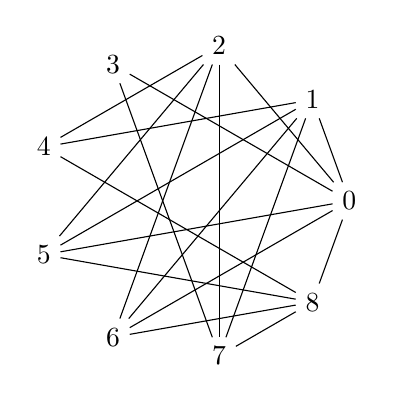
\begin{tikzpicture}
      \draw
        (0.0:2) node (0){0}
        (40.0:2) node (1){1}
        (80.0:2) node (2){2}
        (120.0:2) node (3){3}
        (160.0:2) node (4){4}
        (200.0:2) node (5){5}
        (240.0:2) node (6){6}
        (280.0:2) node (7){7}
        (320.0:2) node (8){8};
      \begin{scope}[-]
        \draw (0) to (1);
        \draw (0) to (2);
        \draw (0) to (3);
        \draw (0) to (5);
        \draw (0) to (6);
        \draw (0) to (8);
        \draw (1) to (4);
        \draw (1) to (5);
        \draw (1) to (6);
        \draw (1) to (7);
        \draw (2) to (4);
        \draw (2) to (5);
        \draw (2) to (6);
        \draw (2) to (7);
        \draw (3) to (7);
        \draw (4) to (8);
        \draw (5) to (8);
        \draw (6) to (8);
        \draw (7) to (8);
      \end{scope}
    \end{tikzpicture}
\end{figure}
\begin{itemize}
\item signature: 111011010011110011110000100001001011
\item g: Graph with 9 nodes and 19 edges
\item order: 9
\item size: 19
\item max degree: 6
\item degrees: 2,3,4,4,4,5,5,5,6
\item is tree: 0
\item is bipartite: 0
\item has bridge: 0
\item is chordal: 0
\item is complete: 0
\item min cycle basis weight: 38
\item min cycle basis size: 11
\item diameter: 3
\item radius: 2
\item is eulerian: 0
\item is planar: 0
\item number of faces: 12
\item is regular: 0
\item p3: 49
\item p4: 14
\item property hash: e6a49ce94870e492a61fa0ff5af59dd9dae919f5e0037e0d873652f6c38f6dbc
\end{itemize}
\newpage
\begin{figure}
  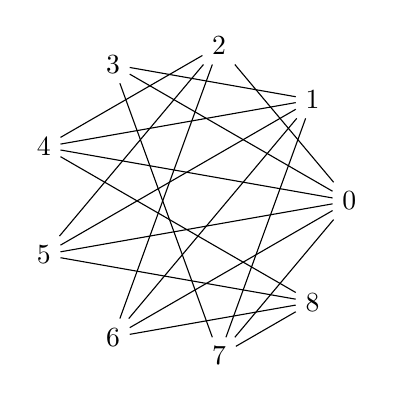
\begin{tikzpicture}
      \draw
        (0.0:2) node (0){0}
        (40.0:2) node (1){1}
        (80.0:2) node (2){2}
        (120.0:2) node (3){3}
        (160.0:2) node (4){4}
        (200.0:2) node (5){5}
        (240.0:2) node (6){6}
        (280.0:2) node (7){7}
        (320.0:2) node (8){8};
      \begin{scope}[-]
        \draw (0) to (2);
        \draw (0) to (3);
        \draw (0) to (4);
        \draw (0) to (5);
        \draw (0) to (6);
        \draw (0) to (7);
        \draw (1) to (3);
        \draw (1) to (4);
        \draw (1) to (5);
        \draw (1) to (6);
        \draw (1) to (7);
        \draw (2) to (4);
        \draw (2) to (5);
        \draw (2) to (6);
        \draw (3) to (7);
        \draw (4) to (8);
        \draw (5) to (8);
        \draw (6) to (8);
        \draw (7) to (8);
      \end{scope}
    \end{tikzpicture}
\end{figure}
\begin{itemize}
\item signature: 011111100111110011100000100001001011
\item g: Graph with 9 nodes and 19 edges
\item order: 9
\item size: 19
\item max degree: 6
\item degrees: 3,4,4,4,4,4,4,5,6
\item is tree: 0
\item is bipartite: 0
\item has bridge: 0
\item is chordal: 0
\item is complete: 0
\item min cycle basis weight: 39
\item min cycle basis size: 11
\item diameter: 2
\item radius: 2
\item is eulerian: 0
\item is planar: 0
\item number of faces: 12
\item is regular: 0
\item p3: 49
\item p4: 21
\item property hash: 99f3e0a23e4fd083ed3493c1f85a05eddd3f071f234f95bad504eb47e6ade3e2
\end{itemize}
\newpage
\begin{figure}
  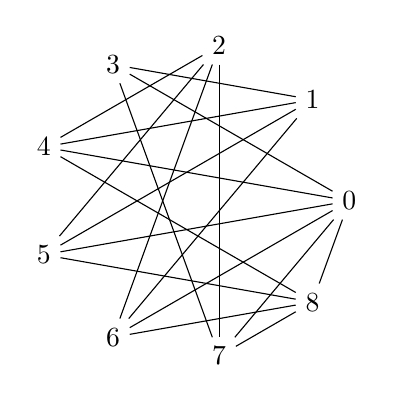
\begin{tikzpicture}
      \draw
        (0.0:2) node (0){0}
        (40.0:2) node (1){1}
        (80.0:2) node (2){2}
        (120.0:2) node (3){3}
        (160.0:2) node (4){4}
        (200.0:2) node (5){5}
        (240.0:2) node (6){6}
        (280.0:2) node (7){7}
        (320.0:2) node (8){8};
      \begin{scope}[-]
        \draw (0) to (3);
        \draw (0) to (4);
        \draw (0) to (5);
        \draw (0) to (6);
        \draw (0) to (7);
        \draw (0) to (8);
        \draw (1) to (3);
        \draw (1) to (4);
        \draw (1) to (5);
        \draw (1) to (6);
        \draw (2) to (4);
        \draw (2) to (5);
        \draw (2) to (6);
        \draw (2) to (7);
        \draw (3) to (7);
        \draw (4) to (8);
        \draw (5) to (8);
        \draw (6) to (8);
        \draw (7) to (8);
      \end{scope}
    \end{tikzpicture}
\end{figure}
\begin{itemize}
\item signature: 001111110111100011110000100001001011
\item g: Graph with 9 nodes and 19 edges
\item order: 9
\item size: 19
\item max degree: 6
\item degrees: 3,4,4,4,4,4,4,5,6
\item is tree: 0
\item is bipartite: 0
\item has bridge: 0
\item is chordal: 0
\item is complete: 0
\item min cycle basis weight: 39
\item min cycle basis size: 11
\item diameter: 2
\item radius: 2
\item is eulerian: 0
\item is planar: 0
\item number of faces: 12
\item is regular: 0
\item p3: 49
\item p4: 30
\item property hash: fa510564bebc17b526c5e016dc896a570cb5ac5f8fd2262dcc541804bf36bdfa
\end{itemize}
\newpage
\begin{figure}
  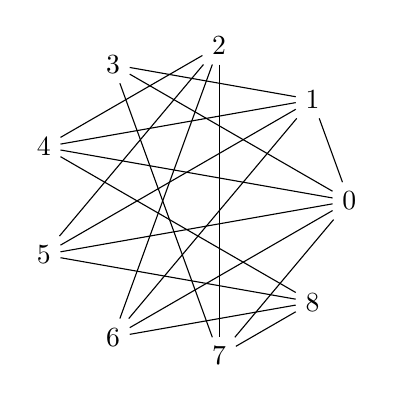
\begin{tikzpicture}
      \draw
        (0.0:2) node (0){0}
        (40.0:2) node (1){1}
        (80.0:2) node (2){2}
        (120.0:2) node (3){3}
        (160.0:2) node (4){4}
        (200.0:2) node (5){5}
        (240.0:2) node (6){6}
        (280.0:2) node (7){7}
        (320.0:2) node (8){8};
      \begin{scope}[-]
        \draw (0) to (1);
        \draw (0) to (3);
        \draw (0) to (4);
        \draw (0) to (5);
        \draw (0) to (6);
        \draw (0) to (7);
        \draw (1) to (3);
        \draw (1) to (4);
        \draw (1) to (5);
        \draw (1) to (6);
        \draw (2) to (4);
        \draw (2) to (5);
        \draw (2) to (6);
        \draw (2) to (7);
        \draw (3) to (7);
        \draw (4) to (8);
        \draw (5) to (8);
        \draw (6) to (8);
        \draw (7) to (8);
      \end{scope}
    \end{tikzpicture}
\end{figure}
\begin{itemize}
\item signature: 101111100111100011110000100001001011
\item g: Graph with 9 nodes and 19 edges
\item order: 9
\item size: 19
\item max degree: 6
\item degrees: 3,4,4,4,4,4,4,5,6
\item is tree: 0
\item is bipartite: 0
\item has bridge: 0
\item is chordal: 0
\item is complete: 0
\item min cycle basis weight: 39
\item min cycle basis size: 11
\item diameter: 2
\item radius: 2
\item is eulerian: 0
\item is planar: 0
\item number of faces: 12
\item is regular: 0
\item p3: 49
\item p4: 31
\item property hash: a23dedb33edfda7ce166f42f2b65c2d73a4f40e355ec4ad96b648dde90bf7d82
\end{itemize}
\newpage
\begin{figure}
  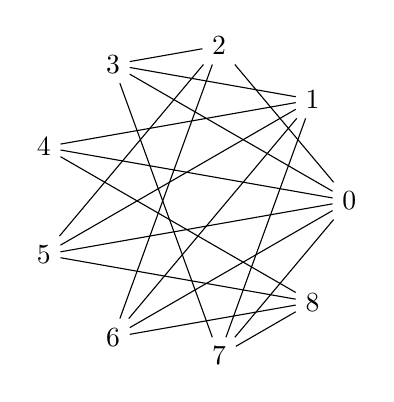
\begin{tikzpicture}
      \draw
        (0.0:2) node (0){0}
        (40.0:2) node (1){1}
        (80.0:2) node (2){2}
        (120.0:2) node (3){3}
        (160.0:2) node (4){4}
        (200.0:2) node (5){5}
        (240.0:2) node (6){6}
        (280.0:2) node (7){7}
        (320.0:2) node (8){8};
      \begin{scope}[-]
        \draw (0) to (2);
        \draw (0) to (3);
        \draw (0) to (4);
        \draw (0) to (5);
        \draw (0) to (6);
        \draw (0) to (7);
        \draw (1) to (3);
        \draw (1) to (4);
        \draw (1) to (5);
        \draw (1) to (6);
        \draw (1) to (7);
        \draw (2) to (3);
        \draw (2) to (5);
        \draw (2) to (6);
        \draw (3) to (7);
        \draw (4) to (8);
        \draw (5) to (8);
        \draw (6) to (8);
        \draw (7) to (8);
      \end{scope}
    \end{tikzpicture}
\end{figure}
\begin{itemize}
\item signature: 011111100111110101100000100001001011
\item g: Graph with 9 nodes and 19 edges
\item order: 9
\item size: 19
\item max degree: 6
\item degrees: 3,4,4,4,4,4,4,5,6
\item is tree: 0
\item is bipartite: 0
\item has bridge: 0
\item is chordal: 0
\item is complete: 0
\item min cycle basis weight: 39
\item min cycle basis size: 11
\item diameter: 2
\item radius: 2
\item is eulerian: 0
\item is planar: 0
\item number of faces: 12
\item is regular: 0
\item p3: 49
\item p4: 27
\item property hash: 32a672d79036acebed9842f8e4e32a344d9a848d0f4ebcfcffac3f93281318d6
\end{itemize}
\newpage
\begin{figure}
  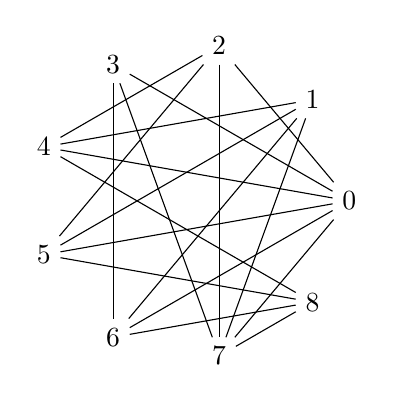
\begin{tikzpicture}
      \draw
        (0.0:2) node (0){0}
        (40.0:2) node (1){1}
        (80.0:2) node (2){2}
        (120.0:2) node (3){3}
        (160.0:2) node (4){4}
        (200.0:2) node (5){5}
        (240.0:2) node (6){6}
        (280.0:2) node (7){7}
        (320.0:2) node (8){8};
      \begin{scope}[-]
        \draw (0) to (2);
        \draw (0) to (3);
        \draw (0) to (4);
        \draw (0) to (5);
        \draw (0) to (6);
        \draw (0) to (7);
        \draw (1) to (4);
        \draw (1) to (5);
        \draw (1) to (6);
        \draw (1) to (7);
        \draw (2) to (4);
        \draw (2) to (5);
        \draw (2) to (7);
        \draw (3) to (6);
        \draw (3) to (7);
        \draw (4) to (8);
        \draw (5) to (8);
        \draw (6) to (8);
        \draw (7) to (8);
      \end{scope}
    \end{tikzpicture}
\end{figure}
\begin{itemize}
\item signature: 011111100011110011010001100001001011
\item g: Graph with 9 nodes and 19 edges
\item order: 9
\item size: 19
\item max degree: 6
\item degrees: 3,4,4,4,4,4,4,5,6
\item is tree: 0
\item is bipartite: 0
\item has bridge: 0
\item is chordal: 0
\item is complete: 0
\item min cycle basis weight: 39
\item min cycle basis size: 11
\item diameter: 2
\item radius: 2
\item is eulerian: 0
\item is planar: 0
\item number of faces: 12
\item is regular: 0
\item p3: 49
\item p4: None
\item property hash: 0a99f125371937789ba3e5a59bbbb6f13ba2771fbdf19c9e8d95b1e91f9e13c4
\end{itemize}
\newpage
\begin{figure}
  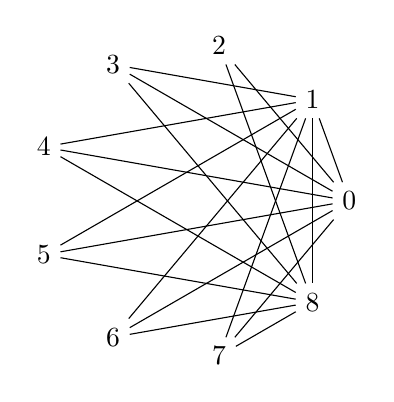
\begin{tikzpicture}
      \draw
        (0.0:2) node (0){0}
        (40.0:2) node (1){1}
        (80.0:2) node (2){2}
        (120.0:2) node (3){3}
        (160.0:2) node (4){4}
        (200.0:2) node (5){5}
        (240.0:2) node (6){6}
        (280.0:2) node (7){7}
        (320.0:2) node (8){8};
      \begin{scope}[-]
        \draw (0) to (1);
        \draw (0) to (2);
        \draw (0) to (3);
        \draw (0) to (4);
        \draw (0) to (5);
        \draw (0) to (6);
        \draw (0) to (7);
        \draw (1) to (3);
        \draw (1) to (4);
        \draw (1) to (5);
        \draw (1) to (6);
        \draw (1) to (7);
        \draw (1) to (8);
        \draw (2) to (8);
        \draw (3) to (8);
        \draw (4) to (8);
        \draw (5) to (8);
        \draw (6) to (8);
        \draw (7) to (8);
      \end{scope}
    \end{tikzpicture}
\end{figure}
\begin{itemize}
\item signature: 111111100111111000001000010001001011
\item g: Graph with 9 nodes and 19 edges
\item order: 9
\item size: 19
\item max degree: 7
\item degrees: 2,3,3,3,3,3,7,7,7
\item is tree: 0
\item is bipartite: 0
\item has bridge: 0
\item is chordal: 0
\item is complete: 0
\item min cycle basis weight: 34
\item min cycle basis size: 11
\item diameter: 2
\item radius: 2
\item is eulerian: 0
\item is planar: 0
\item number of faces: 12
\item is regular: 0
\item p3: 49
\item p4: None
\item property hash: b779b487aae8eca799495924fd05e80de64f7ec7db71040bbf303120bc772bd8
\end{itemize}
\newpage
\begin{figure}
  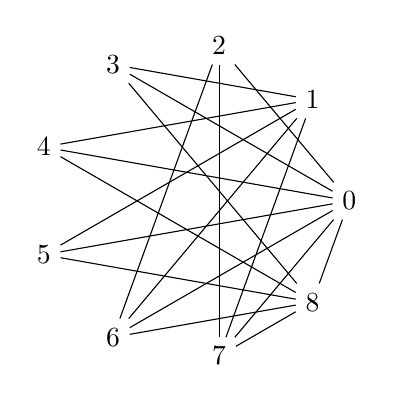
\begin{tikzpicture}
      \draw
        (0.0:2) node (0){0}
        (40.0:2) node (1){1}
        (80.0:2) node (2){2}
        (120.0:2) node (3){3}
        (160.0:2) node (4){4}
        (200.0:2) node (5){5}
        (240.0:2) node (6){6}
        (280.0:2) node (7){7}
        (320.0:2) node (8){8};
      \begin{scope}[-]
        \draw (0) to (2);
        \draw (0) to (3);
        \draw (0) to (4);
        \draw (0) to (5);
        \draw (0) to (6);
        \draw (0) to (7);
        \draw (0) to (8);
        \draw (1) to (3);
        \draw (1) to (4);
        \draw (1) to (5);
        \draw (1) to (6);
        \draw (1) to (7);
        \draw (2) to (6);
        \draw (2) to (7);
        \draw (3) to (8);
        \draw (4) to (8);
        \draw (5) to (8);
        \draw (6) to (8);
        \draw (7) to (8);
      \end{scope}
    \end{tikzpicture}
\end{figure}
\begin{itemize}
\item signature: 011111110111110000110000010001001011
\item g: Graph with 9 nodes and 19 edges
\item order: 9
\item size: 19
\item max degree: 7
\item degrees: 3,3,3,3,4,4,5,6,7
\item is tree: 0
\item is bipartite: 0
\item has bridge: 0
\item is chordal: 0
\item is complete: 0
\item min cycle basis weight: 37
\item min cycle basis size: 11
\item diameter: 2
\item radius: 2
\item is eulerian: 0
\item is planar: 0
\item number of faces: 12
\item is regular: 0
\item p3: 49
\item p4: None
\item property hash: bb04a495f4d6c39b5064bc3199a6038cba960ea07db590f5c3efd0c6eeb0a8c2
\end{itemize}
\newpage
\begin{figure}
  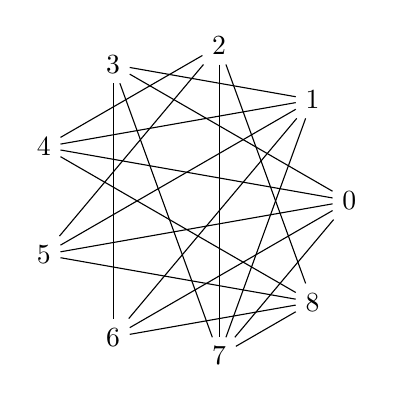
\begin{tikzpicture}
      \draw
        (0.0:2) node (0){0}
        (40.0:2) node (1){1}
        (80.0:2) node (2){2}
        (120.0:2) node (3){3}
        (160.0:2) node (4){4}
        (200.0:2) node (5){5}
        (240.0:2) node (6){6}
        (280.0:2) node (7){7}
        (320.0:2) node (8){8};
      \begin{scope}[-]
        \draw (0) to (3);
        \draw (0) to (4);
        \draw (0) to (5);
        \draw (0) to (6);
        \draw (0) to (7);
        \draw (1) to (3);
        \draw (1) to (4);
        \draw (1) to (5);
        \draw (1) to (6);
        \draw (1) to (7);
        \draw (2) to (4);
        \draw (2) to (5);
        \draw (2) to (7);
        \draw (2) to (8);
        \draw (3) to (6);
        \draw (3) to (7);
        \draw (4) to (8);
        \draw (5) to (8);
        \draw (6) to (8);
        \draw (7) to (8);
      \end{scope}
    \end{tikzpicture}
\end{figure}
\begin{itemize}
\item signature: 001111100111110011011001100001001011
\item g: Graph with 9 nodes and 20 edges
\item order: 9
\item size: 20
\item max degree: 5
\item degrees: 4,4,4,4,4,5,5,5,5
\item is tree: 0
\item is bipartite: 0
\item has bridge: 0
\item is chordal: 0
\item is complete: 0
\item min cycle basis weight: 41
\item min cycle basis size: 12
\item diameter: 2
\item radius: 2
\item is eulerian: 0
\item is planar: 0
\item number of faces: 13
\item is regular: 0
\item p3: 49
\item p4: 24
\item property hash: 07773f8a27912fe3f16e2bcc6f03e0b776278844ea6e8dd86dae4952e273749e
\end{itemize}
\newpage
\begin{figure}
  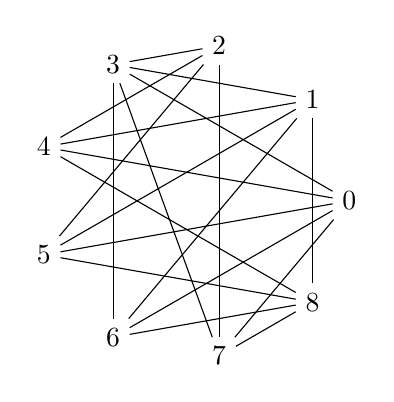
\begin{tikzpicture}
      \draw
        (0.0:2) node (0){0}
        (40.0:2) node (1){1}
        (80.0:2) node (2){2}
        (120.0:2) node (3){3}
        (160.0:2) node (4){4}
        (200.0:2) node (5){5}
        (240.0:2) node (6){6}
        (280.0:2) node (7){7}
        (320.0:2) node (8){8};
      \begin{scope}[-]
        \draw (0) to (3);
        \draw (0) to (4);
        \draw (0) to (5);
        \draw (0) to (6);
        \draw (0) to (7);
        \draw (1) to (3);
        \draw (1) to (4);
        \draw (1) to (5);
        \draw (1) to (6);
        \draw (1) to (8);
        \draw (2) to (3);
        \draw (2) to (4);
        \draw (2) to (5);
        \draw (2) to (7);
        \draw (3) to (6);
        \draw (3) to (7);
        \draw (4) to (8);
        \draw (5) to (8);
        \draw (6) to (8);
        \draw (7) to (8);
      \end{scope}
    \end{tikzpicture}
\end{figure}
\begin{itemize}
\item signature: 001111100111101111010001100001001011
\item g: Graph with 9 nodes and 20 edges
\item order: 9
\item size: 20
\item max degree: 5
\item degrees: 4,4,4,4,4,5,5,5,5
\item is tree: 0
\item is bipartite: 0
\item has bridge: 0
\item is chordal: 0
\item is complete: 0
\item min cycle basis weight: 41
\item min cycle basis size: 12
\item diameter: 2
\item radius: 2
\item is eulerian: 0
\item is planar: 0
\item number of faces: 13
\item is regular: 0
\item p3: 49
\item p4: 30
\item property hash: 81edd25a86b9bb29ac873ef0bd0e00ec8ed4ee46e43ad0a78e3374f996401ff0
\end{itemize}
\newpage
\begin{figure}
  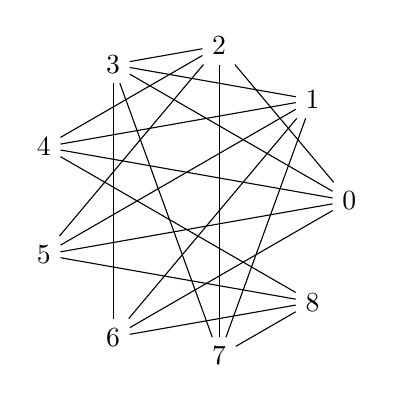
\begin{tikzpicture}
      \draw
        (0.0:2) node (0){0}
        (40.0:2) node (1){1}
        (80.0:2) node (2){2}
        (120.0:2) node (3){3}
        (160.0:2) node (4){4}
        (200.0:2) node (5){5}
        (240.0:2) node (6){6}
        (280.0:2) node (7){7}
        (320.0:2) node (8){8};
      \begin{scope}[-]
        \draw (0) to (2);
        \draw (0) to (3);
        \draw (0) to (4);
        \draw (0) to (5);
        \draw (0) to (6);
        \draw (1) to (3);
        \draw (1) to (4);
        \draw (1) to (5);
        \draw (1) to (6);
        \draw (1) to (7);
        \draw (2) to (3);
        \draw (2) to (4);
        \draw (2) to (5);
        \draw (2) to (7);
        \draw (3) to (6);
        \draw (3) to (7);
        \draw (4) to (8);
        \draw (5) to (8);
        \draw (6) to (8);
        \draw (7) to (8);
      \end{scope}
    \end{tikzpicture}
\end{figure}
\begin{itemize}
\item signature: 011111000111110111010001100001001011
\item g: Graph with 9 nodes and 20 edges
\item order: 9
\item size: 20
\item max degree: 5
\item degrees: 4,4,4,4,4,5,5,5,5
\item is tree: 0
\item is bipartite: 0
\item has bridge: 0
\item is chordal: 0
\item is complete: 0
\item min cycle basis weight: 41
\item min cycle basis size: 12
\item diameter: 2
\item radius: 2
\item is eulerian: 0
\item is planar: 0
\item number of faces: 13
\item is regular: 0
\item p3: 49
\item p4: 33
\item property hash: 300dcb69f18313812c629655ddf21b1597f31d0ad3c60df20f276fd0d8a56d79
\end{itemize}
\newpage
\begin{figure}
  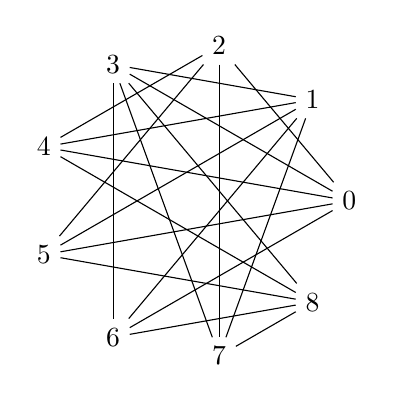
\begin{tikzpicture}
      \draw
        (0.0:2) node (0){0}
        (40.0:2) node (1){1}
        (80.0:2) node (2){2}
        (120.0:2) node (3){3}
        (160.0:2) node (4){4}
        (200.0:2) node (5){5}
        (240.0:2) node (6){6}
        (280.0:2) node (7){7}
        (320.0:2) node (8){8};
      \begin{scope}[-]
        \draw (0) to (2);
        \draw (0) to (3);
        \draw (0) to (4);
        \draw (0) to (5);
        \draw (0) to (6);
        \draw (1) to (3);
        \draw (1) to (4);
        \draw (1) to (5);
        \draw (1) to (6);
        \draw (1) to (7);
        \draw (2) to (4);
        \draw (2) to (5);
        \draw (2) to (7);
        \draw (3) to (6);
        \draw (3) to (7);
        \draw (3) to (8);
        \draw (4) to (8);
        \draw (5) to (8);
        \draw (6) to (8);
        \draw (7) to (8);
      \end{scope}
    \end{tikzpicture}
\end{figure}
\begin{itemize}
\item signature: 011111000111110011010001110001001011
\item g: Graph with 9 nodes and 20 edges
\item order: 9
\item size: 20
\item max degree: 5
\item degrees: 4,4,4,4,4,5,5,5,5
\item is tree: 0
\item is bipartite: 0
\item has bridge: 0
\item is chordal: 0
\item is complete: 0
\item min cycle basis weight: 41
\item min cycle basis size: 12
\item diameter: 2
\item radius: 2
\item is eulerian: 0
\item is planar: 0
\item number of faces: 13
\item is regular: 0
\item p3: 49
\item p4: 28
\item property hash: 9c8aea3c42b542858551908f325e08a787ae3b205d23b2ac43e1be88ab63d2f0
\end{itemize}
\newpage
\begin{figure}
  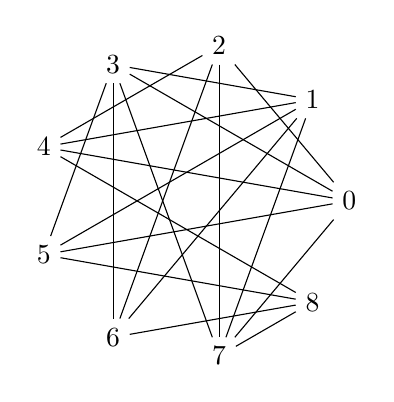
\begin{tikzpicture}
      \draw
        (0.0:2) node (0){0}
        (40.0:2) node (1){1}
        (80.0:2) node (2){2}
        (120.0:2) node (3){3}
        (160.0:2) node (4){4}
        (200.0:2) node (5){5}
        (240.0:2) node (6){6}
        (280.0:2) node (7){7}
        (320.0:2) node (8){8};
      \begin{scope}[-]
        \draw (0) to (2);
        \draw (0) to (3);
        \draw (0) to (4);
        \draw (0) to (5);
        \draw (0) to (7);
        \draw (1) to (3);
        \draw (1) to (4);
        \draw (1) to (5);
        \draw (1) to (6);
        \draw (1) to (7);
        \draw (2) to (4);
        \draw (2) to (6);
        \draw (2) to (7);
        \draw (3) to (5);
        \draw (3) to (6);
        \draw (3) to (7);
        \draw (4) to (8);
        \draw (5) to (8);
        \draw (6) to (8);
        \draw (7) to (8);
      \end{scope}
    \end{tikzpicture}
\end{figure}
\begin{itemize}
\item signature: 011110100111110010110011100001001011
\item g: Graph with 9 nodes and 20 edges
\item order: 9
\item size: 20
\item max degree: 5
\item degrees: 4,4,4,4,4,5,5,5,5
\item is tree: 0
\item is bipartite: 0
\item has bridge: 0
\item is chordal: 0
\item is complete: 0
\item min cycle basis weight: 41
\item min cycle basis size: 12
\item diameter: 2
\item radius: 2
\item is eulerian: 0
\item is planar: 0
\item number of faces: 13
\item is regular: 0
\item p3: 49
\item p4: 30
\item property hash: 81edd25a86b9bb29ac873ef0bd0e00ec8ed4ee46e43ad0a78e3374f996401ff0
\end{itemize}
\newpage
\begin{figure}
  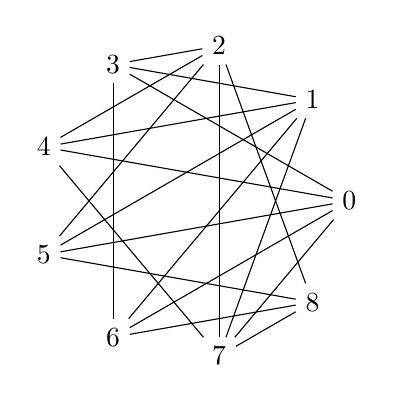
\begin{tikzpicture}
      \draw
        (0.0:2) node (0){0}
        (40.0:2) node (1){1}
        (80.0:2) node (2){2}
        (120.0:2) node (3){3}
        (160.0:2) node (4){4}
        (200.0:2) node (5){5}
        (240.0:2) node (6){6}
        (280.0:2) node (7){7}
        (320.0:2) node (8){8};
      \begin{scope}[-]
        \draw (0) to (3);
        \draw (0) to (4);
        \draw (0) to (5);
        \draw (0) to (6);
        \draw (0) to (7);
        \draw (1) to (3);
        \draw (1) to (4);
        \draw (1) to (5);
        \draw (1) to (6);
        \draw (1) to (7);
        \draw (2) to (3);
        \draw (2) to (4);
        \draw (2) to (5);
        \draw (2) to (7);
        \draw (2) to (8);
        \draw (3) to (6);
        \draw (4) to (7);
        \draw (5) to (8);
        \draw (6) to (8);
        \draw (7) to (8);
      \end{scope}
    \end{tikzpicture}
\end{figure}
\begin{itemize}
\item signature: 001111100111110111011001000010001011
\item g: Graph with 9 nodes and 20 edges
\item order: 9
\item size: 20
\item max degree: 5
\item degrees: 4,4,4,4,4,5,5,5,5
\item is tree: 0
\item is bipartite: 0
\item has bridge: 0
\item is chordal: 0
\item is complete: 0
\item min cycle basis weight: 41
\item min cycle basis size: 12
\item diameter: 2
\item radius: 2
\item is eulerian: 0
\item is planar: 0
\item number of faces: 13
\item is regular: 0
\item p3: 49
\item p4: 28
\item property hash: 9c8aea3c42b542858551908f325e08a787ae3b205d23b2ac43e1be88ab63d2f0
\end{itemize}
\newpage
\begin{figure}
  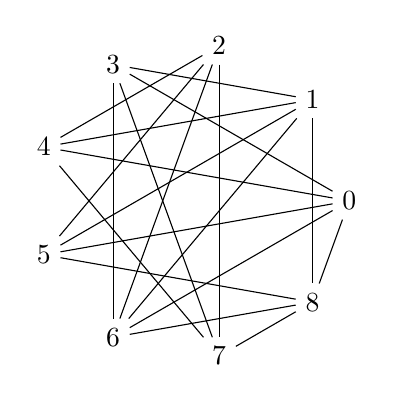
\begin{tikzpicture}
      \draw
        (0.0:2) node (0){0}
        (40.0:2) node (1){1}
        (80.0:2) node (2){2}
        (120.0:2) node (3){3}
        (160.0:2) node (4){4}
        (200.0:2) node (5){5}
        (240.0:2) node (6){6}
        (280.0:2) node (7){7}
        (320.0:2) node (8){8};
      \begin{scope}[-]
        \draw (0) to (3);
        \draw (0) to (4);
        \draw (0) to (5);
        \draw (0) to (6);
        \draw (0) to (8);
        \draw (1) to (3);
        \draw (1) to (4);
        \draw (1) to (5);
        \draw (1) to (6);
        \draw (1) to (8);
        \draw (2) to (4);
        \draw (2) to (5);
        \draw (2) to (6);
        \draw (2) to (7);
        \draw (3) to (6);
        \draw (3) to (7);
        \draw (4) to (7);
        \draw (5) to (8);
        \draw (6) to (8);
        \draw (7) to (8);
      \end{scope}
    \end{tikzpicture}
\end{figure}
\begin{itemize}
\item signature: 001111010111101011110001100010001011
\item g: Graph with 9 nodes and 20 edges
\item order: 9
\item size: 20
\item max degree: 5
\item degrees: 4,4,4,4,4,5,5,5,5
\item is tree: 0
\item is bipartite: 0
\item has bridge: 0
\item is chordal: 0
\item is complete: 0
\item min cycle basis weight: 41
\item min cycle basis size: 12
\item diameter: 2
\item radius: 2
\item is eulerian: 0
\item is planar: 0
\item number of faces: 13
\item is regular: 0
\item p3: 49
\item p4: 30
\item property hash: 81edd25a86b9bb29ac873ef0bd0e00ec8ed4ee46e43ad0a78e3374f996401ff0
\end{itemize}
\newpage
\begin{figure}
  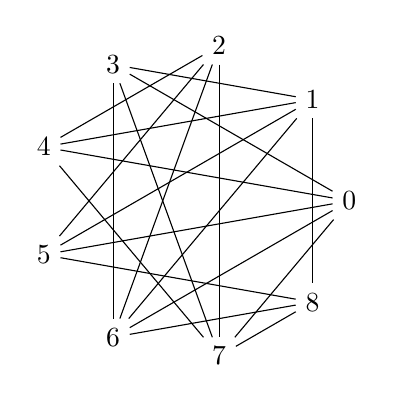
\begin{tikzpicture}
      \draw
        (0.0:2) node (0){0}
        (40.0:2) node (1){1}
        (80.0:2) node (2){2}
        (120.0:2) node (3){3}
        (160.0:2) node (4){4}
        (200.0:2) node (5){5}
        (240.0:2) node (6){6}
        (280.0:2) node (7){7}
        (320.0:2) node (8){8};
      \begin{scope}[-]
        \draw (0) to (3);
        \draw (0) to (4);
        \draw (0) to (5);
        \draw (0) to (6);
        \draw (0) to (7);
        \draw (1) to (3);
        \draw (1) to (4);
        \draw (1) to (5);
        \draw (1) to (6);
        \draw (1) to (8);
        \draw (2) to (4);
        \draw (2) to (5);
        \draw (2) to (6);
        \draw (2) to (7);
        \draw (3) to (6);
        \draw (3) to (7);
        \draw (4) to (7);
        \draw (5) to (8);
        \draw (6) to (8);
        \draw (7) to (8);
      \end{scope}
    \end{tikzpicture}
\end{figure}
\begin{itemize}
\item signature: 001111100111101011110001100010001011
\item g: Graph with 9 nodes and 20 edges
\item order: 9
\item size: 20
\item max degree: 5
\item degrees: 4,4,4,4,4,5,5,5,5
\item is tree: 0
\item is bipartite: 0
\item has bridge: 0
\item is chordal: 0
\item is complete: 0
\item min cycle basis weight: 41
\item min cycle basis size: 12
\item diameter: 2
\item radius: 2
\item is eulerian: 0
\item is planar: 0
\item number of faces: 13
\item is regular: 0
\item p3: 49
\item p4: 30
\item property hash: 81edd25a86b9bb29ac873ef0bd0e00ec8ed4ee46e43ad0a78e3374f996401ff0
\end{itemize}
\newpage
\begin{figure}
  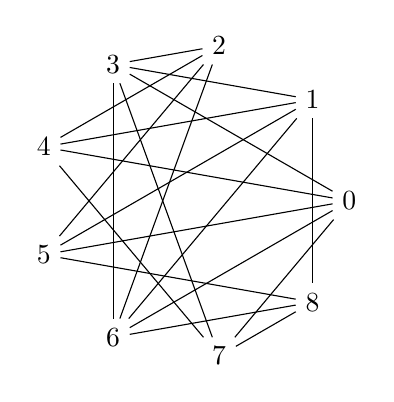
\begin{tikzpicture}
      \draw
        (0.0:2) node (0){0}
        (40.0:2) node (1){1}
        (80.0:2) node (2){2}
        (120.0:2) node (3){3}
        (160.0:2) node (4){4}
        (200.0:2) node (5){5}
        (240.0:2) node (6){6}
        (280.0:2) node (7){7}
        (320.0:2) node (8){8};
      \begin{scope}[-]
        \draw (0) to (3);
        \draw (0) to (4);
        \draw (0) to (5);
        \draw (0) to (6);
        \draw (0) to (7);
        \draw (1) to (3);
        \draw (1) to (4);
        \draw (1) to (5);
        \draw (1) to (6);
        \draw (1) to (8);
        \draw (2) to (3);
        \draw (2) to (4);
        \draw (2) to (5);
        \draw (2) to (6);
        \draw (3) to (6);
        \draw (3) to (7);
        \draw (4) to (7);
        \draw (5) to (8);
        \draw (6) to (8);
        \draw (7) to (8);
      \end{scope}
    \end{tikzpicture}
\end{figure}
\begin{itemize}
\item signature: 001111100111101111100001100010001011
\item g: Graph with 9 nodes and 20 edges
\item order: 9
\item size: 20
\item max degree: 5
\item degrees: 4,4,4,4,4,5,5,5,5
\item is tree: 0
\item is bipartite: 0
\item has bridge: 0
\item is chordal: 0
\item is complete: 0
\item min cycle basis weight: 41
\item min cycle basis size: 12
\item diameter: 2
\item radius: 2
\item is eulerian: 0
\item is planar: 0
\item number of faces: 13
\item is regular: 0
\item p3: 49
\item p4: 30
\item property hash: 81edd25a86b9bb29ac873ef0bd0e00ec8ed4ee46e43ad0a78e3374f996401ff0
\end{itemize}
\newpage
\begin{figure}
  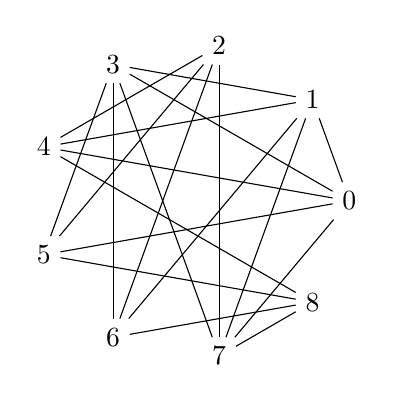
\begin{tikzpicture}
      \draw
        (0.0:2) node (0){0}
        (40.0:2) node (1){1}
        (80.0:2) node (2){2}
        (120.0:2) node (3){3}
        (160.0:2) node (4){4}
        (200.0:2) node (5){5}
        (240.0:2) node (6){6}
        (280.0:2) node (7){7}
        (320.0:2) node (8){8};
      \begin{scope}[-]
        \draw (0) to (1);
        \draw (0) to (3);
        \draw (0) to (4);
        \draw (0) to (5);
        \draw (0) to (7);
        \draw (1) to (3);
        \draw (1) to (4);
        \draw (1) to (6);
        \draw (1) to (7);
        \draw (2) to (4);
        \draw (2) to (5);
        \draw (2) to (6);
        \draw (2) to (7);
        \draw (3) to (5);
        \draw (3) to (6);
        \draw (3) to (7);
        \draw (4) to (8);
        \draw (5) to (8);
        \draw (6) to (8);
        \draw (7) to (8);
      \end{scope}
    \end{tikzpicture}
\end{figure}
\begin{itemize}
\item signature: 101110100110110011110011100001001011
\item g: Graph with 9 nodes and 20 edges
\item order: 9
\item size: 20
\item max degree: 5
\item degrees: 4,4,4,4,4,5,5,5,5
\item is tree: 0
\item is bipartite: 0
\item has bridge: 0
\item is chordal: 0
\item is complete: 0
\item min cycle basis weight: 42
\item min cycle basis size: 12
\item diameter: 2
\item radius: 2
\item is eulerian: 0
\item is planar: 0
\item number of faces: 13
\item is regular: 0
\item p3: 49
\item p4: 33
\item property hash: 74126db7ee557546809f169e3106e8d5426fa5846e090c91d554ee8d790caaba
\end{itemize}
\newpage
\begin{figure}
  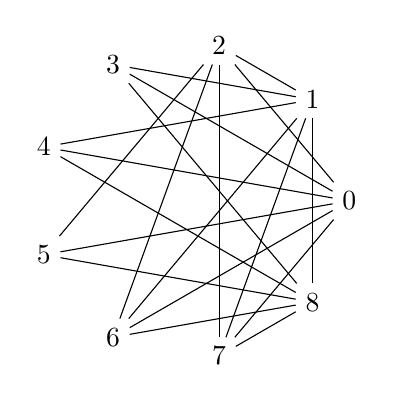
\begin{tikzpicture}
      \draw
        (0.0:2) node (0){0}
        (40.0:2) node (1){1}
        (80.0:2) node (2){2}
        (120.0:2) node (3){3}
        (160.0:2) node (4){4}
        (200.0:2) node (5){5}
        (240.0:2) node (6){6}
        (280.0:2) node (7){7}
        (320.0:2) node (8){8};
      \begin{scope}[-]
        \draw (0) to (2);
        \draw (0) to (3);
        \draw (0) to (4);
        \draw (0) to (5);
        \draw (0) to (6);
        \draw (0) to (7);
        \draw (1) to (2);
        \draw (1) to (3);
        \draw (1) to (4);
        \draw (1) to (6);
        \draw (1) to (7);
        \draw (1) to (8);
        \draw (2) to (5);
        \draw (2) to (6);
        \draw (2) to (7);
        \draw (3) to (8);
        \draw (4) to (8);
        \draw (5) to (8);
        \draw (6) to (8);
        \draw (7) to (8);
      \end{scope}
    \end{tikzpicture}
\end{figure}
\begin{itemize}
\item signature: 011111101110111001110000010001001011
\item g: Graph with 9 nodes and 20 edges
\item order: 9
\item size: 20
\item max degree: 6
\item degrees: 3,3,3,4,4,5,6,6,6
\item is tree: 0
\item is bipartite: 0
\item has bridge: 0
\item is chordal: 0
\item is complete: 0
\item min cycle basis weight: 39
\item min cycle basis size: 12
\item diameter: 2
\item radius: 2
\item is eulerian: 0
\item is planar: 0
\item number of faces: 13
\item is regular: 0
\item p3: 49
\item p4: 16
\item property hash: a2bc26ed6dccfe686fad0da83af24a0e120056c3faa6694dcdc1a5d25253ccd6
\end{itemize}
\newpage
\begin{figure}
  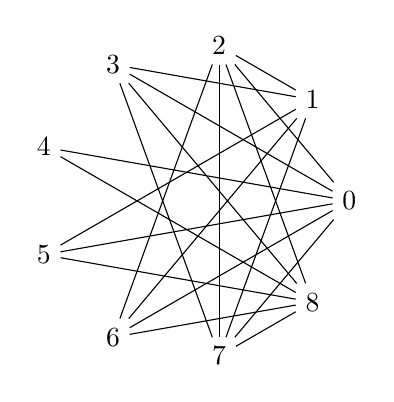
\begin{tikzpicture}
      \draw
        (0.0:2) node (0){0}
        (40.0:2) node (1){1}
        (80.0:2) node (2){2}
        (120.0:2) node (3){3}
        (160.0:2) node (4){4}
        (200.0:2) node (5){5}
        (240.0:2) node (6){6}
        (280.0:2) node (7){7}
        (320.0:2) node (8){8};
      \begin{scope}[-]
        \draw (0) to (2);
        \draw (0) to (3);
        \draw (0) to (4);
        \draw (0) to (5);
        \draw (0) to (6);
        \draw (0) to (7);
        \draw (1) to (2);
        \draw (1) to (3);
        \draw (1) to (5);
        \draw (1) to (6);
        \draw (1) to (7);
        \draw (2) to (6);
        \draw (2) to (7);
        \draw (2) to (8);
        \draw (3) to (7);
        \draw (3) to (8);
        \draw (4) to (8);
        \draw (5) to (8);
        \draw (6) to (8);
        \draw (7) to (8);
      \end{scope}
    \end{tikzpicture}
\end{figure}
\begin{itemize}
\item signature: 011111101101110000111000110001001011
\item g: Graph with 9 nodes and 20 edges
\item order: 9
\item size: 20
\item max degree: 6
\item degrees: 2,3,4,4,5,5,5,6,6
\item is tree: 0
\item is bipartite: 0
\item has bridge: 0
\item is chordal: 0
\item is complete: 0
\item min cycle basis weight: 39
\item min cycle basis size: 12
\item diameter: 3
\item radius: 2
\item is eulerian: 0
\item is planar: 0
\item number of faces: 13
\item is regular: 0
\item p3: 49
\item p4: 11
\item property hash: 09f71114833dd5e9a3a3b061bc89bf852ee7a0658b217149705ce983ec275cb9
\end{itemize}
\newpage
\begin{figure}
  \begin{tikzpicture}
      \draw
        (0.0:2) node (0){0}
        (40.0:2) node (1){1}
        (80.0:2) node (2){2}
        (120.0:2) node (3){3}
        (160.0:2) node (4){4}
        (200.0:2) node (5){5}
        (240.0:2) node (6){6}
        (280.0:2) node (7){7}
        (320.0:2) node (8){8};
      \begin{scope}[-]
        \draw (0) to (2);
        \draw (0) to (3);
        \draw (0) to (4);
        \draw (0) to (5);
        \draw (0) to (6);
        \draw (0) to (7);
        \draw (1) to (3);
        \draw (1) to (4);
        \draw (1) to (5);
        \draw (1) to (6);
        \draw (1) to (7);
        \draw (2) to (5);
        \draw (2) to (6);
        \draw (2) to (7);
        \draw (2) to (8);
        \draw (3) to (7);
        \draw (4) to (8);
        \draw (5) to (8);
        \draw (6) to (8);
        \draw (7) to (8);
      \end{scope}
    \end{tikzpicture}
\end{figure}
\begin{itemize}
\item signature: 011111100111110001111000100001001011
\item g: Graph with 9 nodes and 20 edges
\item order: 9
\item size: 20
\item max degree: 6
\item degrees: 3,3,4,4,5,5,5,5,6
\item is tree: 0
\item is bipartite: 0
\item has bridge: 0
\item is chordal: 0
\item is complete: 0
\item min cycle basis weight: 40
\item min cycle basis size: 12
\item diameter: 2
\item radius: 2
\item is eulerian: 0
\item is planar: 0
\item number of faces: 13
\item is regular: 0
\item p3: 49
\item p4: None
\item property hash: 5a8f5ac1e93337adc808ec25eac37f0405035a8a67bcc6baa784a003abc6590e
\end{itemize}
\newpage
\begin{figure}
  \begin{tikzpicture}
      \draw
        (0.0:2) node (0){0}
        (40.0:2) node (1){1}
        (80.0:2) node (2){2}
        (120.0:2) node (3){3}
        (160.0:2) node (4){4}
        (200.0:2) node (5){5}
        (240.0:2) node (6){6}
        (280.0:2) node (7){7}
        (320.0:2) node (8){8};
      \begin{scope}[-]
        \draw (0) to (2);
        \draw (0) to (3);
        \draw (0) to (4);
        \draw (0) to (5);
        \draw (0) to (6);
        \draw (0) to (7);
        \draw (1) to (2);
        \draw (1) to (3);
        \draw (1) to (4);
        \draw (1) to (5);
        \draw (1) to (6);
        \draw (1) to (7);
        \draw (2) to (4);
        \draw (2) to (5);
        \draw (2) to (6);
        \draw (3) to (7);
        \draw (4) to (8);
        \draw (5) to (8);
        \draw (6) to (8);
        \draw (7) to (8);
      \end{scope}
    \end{tikzpicture}
\end{figure}
\begin{itemize}
\item signature: 011111101111110011100000100001001011
\item g: Graph with 9 nodes and 20 edges
\item order: 9
\item size: 20
\item max degree: 6
\item degrees: 3,4,4,4,4,4,5,6,6
\item is tree: 0
\item is bipartite: 0
\item has bridge: 0
\item is chordal: 0
\item is complete: 0
\item min cycle basis weight: 40
\item min cycle basis size: 12
\item diameter: 2
\item radius: 2
\item is eulerian: 0
\item is planar: 0
\item number of faces: 13
\item is regular: 0
\item p3: 49
\item p4: 14
\item property hash: ccd40dda3b284c134a98379ccf7055148a01893815530baef43a997ea6ab76ed
\end{itemize}
\newpage
\begin{figure}
  \begin{tikzpicture}
      \draw
        (0.0:2) node (0){0}
        (40.0:2) node (1){1}
        (80.0:2) node (2){2}
        (120.0:2) node (3){3}
        (160.0:2) node (4){4}
        (200.0:2) node (5){5}
        (240.0:2) node (6){6}
        (280.0:2) node (7){7}
        (320.0:2) node (8){8};
      \begin{scope}[-]
        \draw (0) to (3);
        \draw (0) to (4);
        \draw (0) to (5);
        \draw (0) to (6);
        \draw (0) to (7);
        \draw (0) to (8);
        \draw (1) to (3);
        \draw (1) to (4);
        \draw (1) to (5);
        \draw (1) to (6);
        \draw (1) to (8);
        \draw (2) to (4);
        \draw (2) to (5);
        \draw (2) to (6);
        \draw (2) to (7);
        \draw (3) to (7);
        \draw (4) to (8);
        \draw (5) to (8);
        \draw (6) to (8);
        \draw (7) to (8);
      \end{scope}
    \end{tikzpicture}
\end{figure}
\begin{itemize}
\item signature: 001111110111101011110000100001001011
\item g: Graph with 9 nodes and 20 edges
\item order: 9
\item size: 20
\item max degree: 6
\item degrees: 3,4,4,4,4,4,5,6,6
\item is tree: 0
\item is bipartite: 0
\item has bridge: 0
\item is chordal: 0
\item is complete: 0
\item min cycle basis weight: 40
\item min cycle basis size: 12
\item diameter: 2
\item radius: 2
\item is eulerian: 0
\item is planar: 0
\item number of faces: 13
\item is regular: 0
\item p3: 49
\item p4: None
\item property hash: b92e7e20cb4cad0f04b62c51acda5e9df2d4e025eb58894566aa74bc565f8791
\end{itemize}
\newpage
\begin{figure}
  \begin{tikzpicture}
      \draw
        (0.0:2) node (0){0}
        (40.0:2) node (1){1}
        (80.0:2) node (2){2}
        (120.0:2) node (3){3}
        (160.0:2) node (4){4}
        (200.0:2) node (5){5}
        (240.0:2) node (6){6}
        (280.0:2) node (7){7}
        (320.0:2) node (8){8};
      \begin{scope}[-]
        \draw (0) to (1);
        \draw (0) to (3);
        \draw (0) to (4);
        \draw (0) to (5);
        \draw (0) to (6);
        \draw (0) to (7);
        \draw (1) to (3);
        \draw (1) to (4);
        \draw (1) to (5);
        \draw (1) to (6);
        \draw (1) to (8);
        \draw (2) to (4);
        \draw (2) to (5);
        \draw (2) to (6);
        \draw (2) to (7);
        \draw (3) to (7);
        \draw (4) to (8);
        \draw (5) to (8);
        \draw (6) to (8);
        \draw (7) to (8);
      \end{scope}
    \end{tikzpicture}
\end{figure}
\begin{itemize}
\item signature: 101111100111101011110000100001001011
\item g: Graph with 9 nodes and 20 edges
\item order: 9
\item size: 20
\item max degree: 6
\item degrees: 3,4,4,4,4,4,5,6,6
\item is tree: 0
\item is bipartite: 0
\item has bridge: 0
\item is chordal: 0
\item is complete: 0
\item min cycle basis weight: 40
\item min cycle basis size: 12
\item diameter: 2
\item radius: 2
\item is eulerian: 0
\item is planar: 0
\item number of faces: 13
\item is regular: 0
\item p3: 49
\item p4: 24
\item property hash: 910482fbd4185b417009e5112c86174f56ed0ca9884d5a037014f0ebfae622b9
\end{itemize}
\newpage
\begin{figure}
  \begin{tikzpicture}
      \draw
        (0.0:2) node (0){0}
        (40.0:2) node (1){1}
        (80.0:2) node (2){2}
        (120.0:2) node (3){3}
        (160.0:2) node (4){4}
        (200.0:2) node (5){5}
        (240.0:2) node (6){6}
        (280.0:2) node (7){7}
        (320.0:2) node (8){8};
      \begin{scope}[-]
        \draw (0) to (2);
        \draw (0) to (3);
        \draw (0) to (5);
        \draw (0) to (6);
        \draw (0) to (7);
        \draw (0) to (8);
        \draw (1) to (3);
        \draw (1) to (4);
        \draw (1) to (5);
        \draw (1) to (6);
        \draw (1) to (7);
        \draw (2) to (4);
        \draw (2) to (5);
        \draw (2) to (6);
        \draw (2) to (7);
        \draw (3) to (7);
        \draw (4) to (8);
        \draw (5) to (8);
        \draw (6) to (8);
        \draw (7) to (8);
      \end{scope}
    \end{tikzpicture}
\end{figure}
\begin{itemize}
\item signature: 011011110111110011110000100001001011
\item g: Graph with 9 nodes and 20 edges
\item order: 9
\item size: 20
\item max degree: 6
\item degrees: 3,3,4,4,5,5,5,5,6
\item is tree: 0
\item is bipartite: 0
\item has bridge: 0
\item is chordal: 0
\item is complete: 0
\item min cycle basis weight: 40
\item min cycle basis size: 12
\item diameter: 2
\item radius: 2
\item is eulerian: 0
\item is planar: 0
\item number of faces: 13
\item is regular: 0
\item p3: 49
\item p4: 22
\item property hash: c7003ef0e9f30a41c2cb1aacf2c736327119a6c89b89d75a7261438dc06bae4f
\end{itemize}
\newpage
\begin{figure}
  \begin{tikzpicture}
      \draw
        (0.0:2) node (0){0}
        (40.0:2) node (1){1}
        (80.0:2) node (2){2}
        (120.0:2) node (3){3}
        (160.0:2) node (4){4}
        (200.0:2) node (5){5}
        (240.0:2) node (6){6}
        (280.0:2) node (7){7}
        (320.0:2) node (8){8};
      \begin{scope}[-]
        \draw (0) to (2);
        \draw (0) to (3);
        \draw (0) to (4);
        \draw (0) to (5);
        \draw (0) to (6);
        \draw (0) to (7);
        \draw (1) to (2);
        \draw (1) to (3);
        \draw (1) to (4);
        \draw (1) to (5);
        \draw (1) to (6);
        \draw (1) to (7);
        \draw (2) to (3);
        \draw (2) to (5);
        \draw (2) to (6);
        \draw (3) to (7);
        \draw (4) to (8);
        \draw (5) to (8);
        \draw (6) to (8);
        \draw (7) to (8);
      \end{scope}
    \end{tikzpicture}
\end{figure}
\begin{itemize}
\item signature: 011111101111110101100000100001001011
\item g: Graph with 9 nodes and 20 edges
\item order: 9
\item size: 20
\item max degree: 6
\item degrees: 3,4,4,4,4,4,5,6,6
\item is tree: 0
\item is bipartite: 0
\item has bridge: 0
\item is chordal: 0
\item is complete: 0
\item min cycle basis weight: 40
\item min cycle basis size: 12
\item diameter: 2
\item radius: 2
\item is eulerian: 0
\item is planar: 0
\item number of faces: 13
\item is regular: 0
\item p3: 49
\item p4: 22
\item property hash: 531e7882ca6b56288389f8d328fdf915a64db0d05687178bf54abb03a97c5493
\end{itemize}
\newpage
\begin{figure}
  \begin{tikzpicture}
      \draw
        (0.0:2) node (0){0}
        (40.0:2) node (1){1}
        (80.0:2) node (2){2}
        (120.0:2) node (3){3}
        (160.0:2) node (4){4}
        (200.0:2) node (5){5}
        (240.0:2) node (6){6}
        (280.0:2) node (7){7}
        (320.0:2) node (8){8};
      \begin{scope}[-]
        \draw (0) to (3);
        \draw (0) to (4);
        \draw (0) to (5);
        \draw (0) to (6);
        \draw (0) to (7);
        \draw (0) to (8);
        \draw (1) to (3);
        \draw (1) to (4);
        \draw (1) to (5);
        \draw (1) to (6);
        \draw (1) to (7);
        \draw (2) to (3);
        \draw (2) to (5);
        \draw (2) to (6);
        \draw (2) to (8);
        \draw (3) to (7);
        \draw (4) to (8);
        \draw (5) to (8);
        \draw (6) to (8);
        \draw (7) to (8);
      \end{scope}
    \end{tikzpicture}
\end{figure}
\begin{itemize}
\item signature: 001111110111110101101000100001001011
\item g: Graph with 9 nodes and 20 edges
\item order: 9
\item size: 20
\item max degree: 6
\item degrees: 3,4,4,4,4,4,5,6,6
\item is tree: 0
\item is bipartite: 0
\item has bridge: 0
\item is chordal: 0
\item is complete: 0
\item min cycle basis weight: 40
\item min cycle basis size: 12
\item diameter: 2
\item radius: 2
\item is eulerian: 0
\item is planar: 0
\item number of faces: 13
\item is regular: 0
\item p3: 49
\item p4: 23
\item property hash: aeb37849df3b0e4654dae0da35211c9a239369739aae07d43544647ec6fee50c
\end{itemize}
\newpage
\begin{figure}
  \begin{tikzpicture}
      \draw
        (0.0:2) node (0){0}
        (40.0:2) node (1){1}
        (80.0:2) node (2){2}
        (120.0:2) node (3){3}
        (160.0:2) node (4){4}
        (200.0:2) node (5){5}
        (240.0:2) node (6){6}
        (280.0:2) node (7){7}
        (320.0:2) node (8){8};
      \begin{scope}[-]
        \draw (0) to (2);
        \draw (0) to (3);
        \draw (0) to (4);
        \draw (0) to (5);
        \draw (0) to (6);
        \draw (0) to (7);
        \draw (1) to (2);
        \draw (1) to (3);
        \draw (1) to (4);
        \draw (1) to (6);
        \draw (1) to (7);
        \draw (2) to (5);
        \draw (2) to (6);
        \draw (2) to (7);
        \draw (3) to (7);
        \draw (3) to (8);
        \draw (4) to (8);
        \draw (5) to (8);
        \draw (6) to (8);
        \draw (7) to (8);
      \end{scope}
    \end{tikzpicture}
\end{figure}
\begin{itemize}
\item signature: 011111101110110001110000110001001011
\item g: Graph with 9 nodes and 20 edges
\item order: 9
\item size: 20
\item max degree: 6
\item degrees: 3,3,4,4,5,5,5,5,6
\item is tree: 0
\item is bipartite: 0
\item has bridge: 0
\item is chordal: 0
\item is complete: 0
\item min cycle basis weight: 40
\item min cycle basis size: 12
\item diameter: 2
\item radius: 2
\item is eulerian: 0
\item is planar: 0
\item number of faces: 13
\item is regular: 0
\item p3: 49
\item p4: 22
\item property hash: c7003ef0e9f30a41c2cb1aacf2c736327119a6c89b89d75a7261438dc06bae4f
\end{itemize}
\newpage
\begin{figure}
  \begin{tikzpicture}
      \draw
        (0.0:2) node (0){0}
        (40.0:2) node (1){1}
        (80.0:2) node (2){2}
        (120.0:2) node (3){3}
        (160.0:2) node (4){4}
        (200.0:2) node (5){5}
        (240.0:2) node (6){6}
        (280.0:2) node (7){7}
        (320.0:2) node (8){8};
      \begin{scope}[-]
        \draw (0) to (2);
        \draw (0) to (3);
        \draw (0) to (4);
        \draw (0) to (5);
        \draw (0) to (6);
        \draw (0) to (7);
        \draw (1) to (3);
        \draw (1) to (4);
        \draw (1) to (5);
        \draw (1) to (6);
        \draw (1) to (7);
        \draw (2) to (6);
        \draw (2) to (7);
        \draw (2) to (8);
        \draw (3) to (6);
        \draw (3) to (7);
        \draw (4) to (8);
        \draw (5) to (8);
        \draw (6) to (8);
        \draw (7) to (8);
      \end{scope}
    \end{tikzpicture}
\end{figure}
\begin{itemize}
\item signature: 011111100111110000111001100001001011
\item g: Graph with 9 nodes and 20 edges
\item order: 9
\item size: 20
\item max degree: 6
\item degrees: 3,3,4,4,5,5,5,5,6
\item is tree: 0
\item is bipartite: 0
\item has bridge: 0
\item is chordal: 0
\item is complete: 0
\item min cycle basis weight: 40
\item min cycle basis size: 12
\item diameter: 2
\item radius: 2
\item is eulerian: 0
\item is planar: 0
\item number of faces: 13
\item is regular: 0
\item p3: 49
\item p4: None
\item property hash: 5a8f5ac1e93337adc808ec25eac37f0405035a8a67bcc6baa784a003abc6590e
\end{itemize}
\newpage
\begin{figure}
  \begin{tikzpicture}
      \draw
        (0.0:2) node (0){0}
        (40.0:2) node (1){1}
        (80.0:2) node (2){2}
        (120.0:2) node (3){3}
        (160.0:2) node (4){4}
        (200.0:2) node (5){5}
        (240.0:2) node (6){6}
        (280.0:2) node (7){7}
        (320.0:2) node (8){8};
      \begin{scope}[-]
        \draw (0) to (2);
        \draw (0) to (3);
        \draw (0) to (4);
        \draw (0) to (5);
        \draw (0) to (6);
        \draw (0) to (7);
        \draw (1) to (2);
        \draw (1) to (3);
        \draw (1) to (4);
        \draw (1) to (5);
        \draw (1) to (7);
        \draw (2) to (6);
        \draw (2) to (7);
        \draw (2) to (8);
        \draw (3) to (6);
        \draw (3) to (7);
        \draw (4) to (8);
        \draw (5) to (8);
        \draw (6) to (8);
        \draw (7) to (8);
      \end{scope}
    \end{tikzpicture}
\end{figure}
\begin{itemize}
\item signature: 011111101111010000111001100001001011
\item g: Graph with 9 nodes and 20 edges
\item order: 9
\item size: 20
\item max degree: 6
\item degrees: 3,3,4,4,5,5,5,5,6
\item is tree: 0
\item is bipartite: 0
\item has bridge: 0
\item is chordal: 0
\item is complete: 0
\item min cycle basis weight: 40
\item min cycle basis size: 12
\item diameter: 2
\item radius: 2
\item is eulerian: 0
\item is planar: 0
\item number of faces: 13
\item is regular: 0
\item p3: 49
\item p4: None
\item property hash: 5a8f5ac1e93337adc808ec25eac37f0405035a8a67bcc6baa784a003abc6590e
\end{itemize}
\newpage
\begin{figure}
  \begin{tikzpicture}
      \draw
        (0.0:2) node (0){0}
        (40.0:2) node (1){1}
        (80.0:2) node (2){2}
        (120.0:2) node (3){3}
        (160.0:2) node (4){4}
        (200.0:2) node (5){5}
        (240.0:2) node (6){6}
        (280.0:2) node (7){7}
        (320.0:2) node (8){8};
      \begin{scope}[-]
        \draw (0) to (2);
        \draw (0) to (3);
        \draw (0) to (4);
        \draw (0) to (5);
        \draw (0) to (6);
        \draw (0) to (7);
        \draw (1) to (2);
        \draw (1) to (3);
        \draw (1) to (4);
        \draw (1) to (5);
        \draw (1) to (6);
        \draw (1) to (7);
        \draw (2) to (5);
        \draw (2) to (7);
        \draw (3) to (6);
        \draw (3) to (7);
        \draw (4) to (8);
        \draw (5) to (8);
        \draw (6) to (8);
        \draw (7) to (8);
      \end{scope}
    \end{tikzpicture}
\end{figure}
\begin{itemize}
\item signature: 011111101111110001010001100001001011
\item g: Graph with 9 nodes and 20 edges
\item order: 9
\item size: 20
\item max degree: 6
\item degrees: 3,4,4,4,4,4,5,6,6
\item is tree: 0
\item is bipartite: 0
\item has bridge: 0
\item is chordal: 0
\item is complete: 0
\item min cycle basis weight: 40
\item min cycle basis size: 12
\item diameter: 2
\item radius: 2
\item is eulerian: 0
\item is planar: 0
\item number of faces: 13
\item is regular: 0
\item p3: 49
\item p4: None
\item property hash: b92e7e20cb4cad0f04b62c51acda5e9df2d4e025eb58894566aa74bc565f8791
\end{itemize}
\newpage
\begin{figure}
  \begin{tikzpicture}
      \draw
        (0.0:2) node (0){0}
        (40.0:2) node (1){1}
        (80.0:2) node (2){2}
        (120.0:2) node (3){3}
        (160.0:2) node (4){4}
        (200.0:2) node (5){5}
        (240.0:2) node (6){6}
        (280.0:2) node (7){7}
        (320.0:2) node (8){8};
      \begin{scope}[-]
        \draw (0) to (2);
        \draw (0) to (3);
        \draw (0) to (4);
        \draw (0) to (5);
        \draw (0) to (6);
        \draw (0) to (7);
        \draw (1) to (2);
        \draw (1) to (4);
        \draw (1) to (5);
        \draw (1) to (6);
        \draw (1) to (7);
        \draw (2) to (5);
        \draw (2) to (7);
        \draw (2) to (8);
        \draw (3) to (6);
        \draw (3) to (7);
        \draw (4) to (8);
        \draw (5) to (8);
        \draw (6) to (8);
        \draw (7) to (8);
      \end{scope}
    \end{tikzpicture}
\end{figure}
\begin{itemize}
\item signature: 011111101011110001011001100001001011
\item g: Graph with 9 nodes and 20 edges
\item order: 9
\item size: 20
\item max degree: 6
\item degrees: 3,3,4,4,5,5,5,5,6
\item is tree: 0
\item is bipartite: 0
\item has bridge: 0
\item is chordal: 0
\item is complete: 0
\item min cycle basis weight: 40
\item min cycle basis size: 12
\item diameter: 2
\item radius: 2
\item is eulerian: 0
\item is planar: 0
\item number of faces: 13
\item is regular: 0
\item p3: 49
\item p4: None
\item property hash: 5a8f5ac1e93337adc808ec25eac37f0405035a8a67bcc6baa784a003abc6590e
\end{itemize}
\newpage
\begin{figure}
  \begin{tikzpicture}
      \draw
        (0.0:2) node (0){0}
        (40.0:2) node (1){1}
        (80.0:2) node (2){2}
        (120.0:2) node (3){3}
        (160.0:2) node (4){4}
        (200.0:2) node (5){5}
        (240.0:2) node (6){6}
        (280.0:2) node (7){7}
        (320.0:2) node (8){8};
      \begin{scope}[-]
        \draw (0) to (1);
        \draw (0) to (2);
        \draw (0) to (3);
        \draw (0) to (4);
        \draw (0) to (5);
        \draw (0) to (8);
        \draw (1) to (3);
        \draw (1) to (4);
        \draw (1) to (5);
        \draw (1) to (6);
        \draw (1) to (7);
        \draw (2) to (5);
        \draw (2) to (6);
        \draw (2) to (7);
        \draw (3) to (6);
        \draw (3) to (7);
        \draw (4) to (8);
        \draw (5) to (8);
        \draw (6) to (8);
        \draw (7) to (8);
      \end{scope}
    \end{tikzpicture}
\end{figure}
\begin{itemize}
\item signature: 111110010111110001110001100001001011
\item g: Graph with 9 nodes and 20 edges
\item order: 9
\item size: 20
\item max degree: 6
\item degrees: 3,4,4,4,4,4,5,6,6
\item is tree: 0
\item is bipartite: 0
\item has bridge: 0
\item is chordal: 0
\item is complete: 0
\item min cycle basis weight: 40
\item min cycle basis size: 12
\item diameter: 2
\item radius: 2
\item is eulerian: 0
\item is planar: 0
\item number of faces: 13
\item is regular: 0
\item p3: 49
\item p4: None
\item property hash: b92e7e20cb4cad0f04b62c51acda5e9df2d4e025eb58894566aa74bc565f8791
\end{itemize}
\newpage
\begin{figure}
  \begin{tikzpicture}
      \draw
        (0.0:2) node (0){0}
        (40.0:2) node (1){1}
        (80.0:2) node (2){2}
        (120.0:2) node (3){3}
        (160.0:2) node (4){4}
        (200.0:2) node (5){5}
        (240.0:2) node (6){6}
        (280.0:2) node (7){7}
        (320.0:2) node (8){8};
      \begin{scope}[-]
        \draw (0) to (2);
        \draw (0) to (3);
        \draw (0) to (4);
        \draw (0) to (5);
        \draw (0) to (6);
        \draw (0) to (7);
        \draw (1) to (2);
        \draw (1) to (4);
        \draw (1) to (5);
        \draw (1) to (6);
        \draw (1) to (7);
        \draw (2) to (5);
        \draw (2) to (6);
        \draw (2) to (7);
        \draw (3) to (6);
        \draw (3) to (7);
        \draw (4) to (8);
        \draw (5) to (8);
        \draw (6) to (8);
        \draw (7) to (8);
      \end{scope}
    \end{tikzpicture}
\end{figure}
\begin{itemize}
\item signature: 011111101011110001110001100001001011
\item g: Graph with 9 nodes and 20 edges
\item order: 9
\item size: 20
\item max degree: 6
\item degrees: 3,3,4,4,5,5,5,5,6
\item is tree: 0
\item is bipartite: 0
\item has bridge: 0
\item is chordal: 0
\item is complete: 0
\item min cycle basis weight: 40
\item min cycle basis size: 12
\item diameter: 2
\item radius: 2
\item is eulerian: 0
\item is planar: 0
\item number of faces: 13
\item is regular: 0
\item p3: 49
\item p4: None
\item property hash: 5a8f5ac1e93337adc808ec25eac37f0405035a8a67bcc6baa784a003abc6590e
\end{itemize}
\newpage
\begin{figure}
  \begin{tikzpicture}
      \draw
        (0.0:2) node (0){0}
        (40.0:2) node (1){1}
        (80.0:2) node (2){2}
        (120.0:2) node (3){3}
        (160.0:2) node (4){4}
        (200.0:2) node (5){5}
        (240.0:2) node (6){6}
        (280.0:2) node (7){7}
        (320.0:2) node (8){8};
      \begin{scope}[-]
        \draw (0) to (2);
        \draw (0) to (3);
        \draw (0) to (4);
        \draw (0) to (5);
        \draw (0) to (6);
        \draw (1) to (2);
        \draw (1) to (3);
        \draw (1) to (4);
        \draw (1) to (5);
        \draw (1) to (6);
        \draw (2) to (5);
        \draw (2) to (7);
        \draw (2) to (8);
        \draw (3) to (6);
        \draw (3) to (7);
        \draw (3) to (8);
        \draw (4) to (8);
        \draw (5) to (8);
        \draw (6) to (8);
        \draw (7) to (8);
      \end{scope}
    \end{tikzpicture}
\end{figure}
\begin{itemize}
\item signature: 011111001111100001011001110001001011
\item g: Graph with 9 nodes and 20 edges
\item order: 9
\item size: 20
\item max degree: 6
\item degrees: 3,3,4,4,5,5,5,5,6
\item is tree: 0
\item is bipartite: 0
\item has bridge: 0
\item is chordal: 0
\item is complete: 0
\item min cycle basis weight: 40
\item min cycle basis size: 12
\item diameter: 2
\item radius: 2
\item is eulerian: 0
\item is planar: 0
\item number of faces: 13
\item is regular: 0
\item p3: 49
\item p4: None
\item property hash: 5a8f5ac1e93337adc808ec25eac37f0405035a8a67bcc6baa784a003abc6590e
\end{itemize}
\newpage
\begin{figure}
  \begin{tikzpicture}
      \draw
        (0.0:2) node (0){0}
        (40.0:2) node (1){1}
        (80.0:2) node (2){2}
        (120.0:2) node (3){3}
        (160.0:2) node (4){4}
        (200.0:2) node (5){5}
        (240.0:2) node (6){6}
        (280.0:2) node (7){7}
        (320.0:2) node (8){8};
      \begin{scope}[-]
        \draw (0) to (3);
        \draw (0) to (4);
        \draw (0) to (5);
        \draw (0) to (6);
        \draw (0) to (7);
        \draw (0) to (8);
        \draw (1) to (3);
        \draw (1) to (4);
        \draw (1) to (5);
        \draw (1) to (6);
        \draw (1) to (7);
        \draw (2) to (5);
        \draw (2) to (6);
        \draw (2) to (7);
        \draw (3) to (6);
        \draw (3) to (7);
        \draw (4) to (8);
        \draw (5) to (8);
        \draw (6) to (8);
        \draw (7) to (8);
      \end{scope}
    \end{tikzpicture}
\end{figure}
\begin{itemize}
\item signature: 001111110111110001110001100001001011
\item g: Graph with 9 nodes and 20 edges
\item order: 9
\item size: 20
\item max degree: 6
\item degrees: 3,3,4,4,5,5,5,5,6
\item is tree: 0
\item is bipartite: 0
\item has bridge: 0
\item is chordal: 0
\item is complete: 0
\item min cycle basis weight: 40
\item min cycle basis size: 12
\item diameter: 3
\item radius: 2
\item is eulerian: 0
\item is planar: 0
\item number of faces: 13
\item is regular: 0
\item p3: 49
\item p4: 20
\item property hash: 0fddb1e5f66f03ab063fc3af5543f00898d8808bcb171732ae2229063d80e091
\end{itemize}
\newpage
\begin{figure}
  \begin{tikzpicture}
      \draw
        (0.0:2) node (0){0}
        (40.0:2) node (1){1}
        (80.0:2) node (2){2}
        (120.0:2) node (3){3}
        (160.0:2) node (4){4}
        (200.0:2) node (5){5}
        (240.0:2) node (6){6}
        (280.0:2) node (7){7}
        (320.0:2) node (8){8};
      \begin{scope}[-]
        \draw (0) to (2);
        \draw (0) to (3);
        \draw (0) to (5);
        \draw (0) to (6);
        \draw (0) to (7);
        \draw (0) to (8);
        \draw (1) to (4);
        \draw (1) to (5);
        \draw (1) to (6);
        \draw (1) to (7);
        \draw (2) to (4);
        \draw (2) to (5);
        \draw (2) to (6);
        \draw (2) to (7);
        \draw (3) to (6);
        \draw (3) to (7);
        \draw (4) to (8);
        \draw (5) to (8);
        \draw (6) to (8);
        \draw (7) to (8);
      \end{scope}
    \end{tikzpicture}
\end{figure}
\begin{itemize}
\item signature: 011011110011110011110001100001001011
\item g: Graph with 9 nodes and 20 edges
\item order: 9
\item size: 20
\item max degree: 6
\item degrees: 3,3,4,4,5,5,5,5,6
\item is tree: 0
\item is bipartite: 0
\item has bridge: 0
\item is chordal: 0
\item is complete: 0
\item min cycle basis weight: 40
\item min cycle basis size: 12
\item diameter: 3
\item radius: 2
\item is eulerian: 0
\item is planar: 0
\item number of faces: 13
\item is regular: 0
\item p3: 49
\item p4: 20
\item property hash: 0fddb1e5f66f03ab063fc3af5543f00898d8808bcb171732ae2229063d80e091
\end{itemize}
\newpage
\begin{figure}
  \begin{tikzpicture}
      \draw
        (0.0:2) node (0){0}
        (40.0:2) node (1){1}
        (80.0:2) node (2){2}
        (120.0:2) node (3){3}
        (160.0:2) node (4){4}
        (200.0:2) node (5){5}
        (240.0:2) node (6){6}
        (280.0:2) node (7){7}
        (320.0:2) node (8){8};
      \begin{scope}[-]
        \draw (0) to (3);
        \draw (0) to (4);
        \draw (0) to (5);
        \draw (0) to (6);
        \draw (0) to (7);
        \draw (1) to (3);
        \draw (1) to (4);
        \draw (1) to (6);
        \draw (1) to (7);
        \draw (2) to (3);
        \draw (2) to (5);
        \draw (2) to (6);
        \draw (2) to (7);
        \draw (3) to (6);
        \draw (3) to (7);
        \draw (3) to (8);
        \draw (4) to (8);
        \draw (5) to (8);
        \draw (6) to (8);
        \draw (7) to (8);
      \end{scope}
    \end{tikzpicture}
\end{figure}
\begin{itemize}
\item signature: 001111100110110101110001110001001011
\item g: Graph with 9 nodes and 20 edges
\item order: 9
\item size: 20
\item max degree: 6
\item degrees: 3,3,4,4,5,5,5,5,6
\item is tree: 0
\item is bipartite: 0
\item has bridge: 0
\item is chordal: 0
\item is complete: 0
\item min cycle basis weight: 40
\item min cycle basis size: 12
\item diameter: 3
\item radius: 2
\item is eulerian: 0
\item is planar: 0
\item number of faces: 13
\item is regular: 0
\item p3: 49
\item p4: None
\item property hash: 36d244d25f406b0b7a11483b00e482da9b952b0d26940dc45d4e3fa084d2c00d
\end{itemize}
\newpage
\begin{figure}
  \begin{tikzpicture}
      \draw
        (0.0:2) node (0){0}
        (40.0:2) node (1){1}
        (80.0:2) node (2){2}
        (120.0:2) node (3){3}
        (160.0:2) node (4){4}
        (200.0:2) node (5){5}
        (240.0:2) node (6){6}
        (280.0:2) node (7){7}
        (320.0:2) node (8){8};
      \begin{scope}[-]
        \draw (0) to (2);
        \draw (0) to (4);
        \draw (0) to (5);
        \draw (0) to (6);
        \draw (0) to (7);
        \draw (1) to (2);
        \draw (1) to (4);
        \draw (1) to (6);
        \draw (1) to (7);
        \draw (2) to (5);
        \draw (2) to (6);
        \draw (2) to (7);
        \draw (2) to (8);
        \draw (3) to (5);
        \draw (3) to (6);
        \draw (3) to (7);
        \draw (4) to (8);
        \draw (5) to (8);
        \draw (6) to (8);
        \draw (7) to (8);
      \end{scope}
    \end{tikzpicture}
\end{figure}
\begin{itemize}
\item signature: 010111101010110001111011100001001011
\item g: Graph with 9 nodes and 20 edges
\item order: 9
\item size: 20
\item max degree: 6
\item degrees: 3,3,4,4,5,5,5,5,6
\item is tree: 0
\item is bipartite: 0
\item has bridge: 0
\item is chordal: 0
\item is complete: 0
\item min cycle basis weight: 40
\item min cycle basis size: 12
\item diameter: 3
\item radius: 2
\item is eulerian: 0
\item is planar: 0
\item number of faces: 13
\item is regular: 0
\item p3: 49
\item p4: None
\item property hash: 36d244d25f406b0b7a11483b00e482da9b952b0d26940dc45d4e3fa084d2c00d
\end{itemize}
\newpage
\begin{figure}
  \begin{tikzpicture}
      \draw
        (0.0:2) node (0){0}
        (40.0:2) node (1){1}
        (80.0:2) node (2){2}
        (120.0:2) node (3){3}
        (160.0:2) node (4){4}
        (200.0:2) node (5){5}
        (240.0:2) node (6){6}
        (280.0:2) node (7){7}
        (320.0:2) node (8){8};
      \begin{scope}[-]
        \draw (0) to (2);
        \draw (0) to (3);
        \draw (0) to (4);
        \draw (0) to (5);
        \draw (0) to (6);
        \draw (0) to (7);
        \draw (1) to (3);
        \draw (1) to (4);
        \draw (1) to (5);
        \draw (1) to (6);
        \draw (1) to (7);
        \draw (2) to (3);
        \draw (2) to (6);
        \draw (2) to (7);
        \draw (2) to (8);
        \draw (3) to (7);
        \draw (4) to (8);
        \draw (5) to (8);
        \draw (6) to (8);
        \draw (7) to (8);
      \end{scope}
    \end{tikzpicture}
\end{figure}
\begin{itemize}
\item signature: 011111100111110100111000100001001011
\item g: Graph with 9 nodes and 20 edges
\item order: 9
\item size: 20
\item max degree: 6
\item degrees: 3,3,4,4,5,5,5,5,6
\item is tree: 0
\item is bipartite: 0
\item has bridge: 0
\item is chordal: 0
\item is complete: 0
\item min cycle basis weight: 41
\item min cycle basis size: 12
\item diameter: 2
\item radius: 2
\item is eulerian: 0
\item is planar: 0
\item number of faces: 13
\item is regular: 0
\item p3: 49
\item p4: None
\item property hash: b9676bfa1288d68bc37574a7f77baca43b05217eecaab742177d1e1aa9c6bba2
\end{itemize}
\newpage
\begin{figure}
  \begin{tikzpicture}
      \draw
        (0.0:2) node (0){0}
        (40.0:2) node (1){1}
        (80.0:2) node (2){2}
        (120.0:2) node (3){3}
        (160.0:2) node (4){4}
        (200.0:2) node (5){5}
        (240.0:2) node (6){6}
        (280.0:2) node (7){7}
        (320.0:2) node (8){8};
      \begin{scope}[-]
        \draw (0) to (1);
        \draw (0) to (2);
        \draw (0) to (3);
        \draw (0) to (4);
        \draw (0) to (5);
        \draw (0) to (6);
        \draw (0) to (7);
        \draw (1) to (2);
        \draw (1) to (3);
        \draw (1) to (4);
        \draw (1) to (5);
        \draw (1) to (7);
        \draw (2) to (6);
        \draw (2) to (7);
        \draw (2) to (8);
        \draw (3) to (8);
        \draw (4) to (8);
        \draw (5) to (8);
        \draw (6) to (8);
        \draw (7) to (8);
      \end{scope}
    \end{tikzpicture}
\end{figure}
\begin{itemize}
\item signature: 111111101111010000111000010001001011
\item g: Graph with 9 nodes and 20 edges
\item order: 9
\item size: 20
\item max degree: 7
\item degrees: 3,3,3,3,4,5,6,6,7
\item is tree: 0
\item is bipartite: 0
\item has bridge: 0
\item is chordal: 0
\item is complete: 0
\item min cycle basis weight: 39
\item min cycle basis size: 12
\item diameter: 2
\item radius: 2
\item is eulerian: 0
\item is planar: 0
\item number of faces: 13
\item is regular: 0
\item p3: 49
\item p4: None
\item property hash: bd28a9433f3194a9865b62d06a0786538e48857970439ce7f0bee7ca2cefae00
\end{itemize}
\newpage
\begin{figure}
  \begin{tikzpicture}
      \draw
        (0.0:2) node (0){0}
        (40.0:2) node (1){1}
        (80.0:2) node (2){2}
        (120.0:2) node (3){3}
        (160.0:2) node (4){4}
        (200.0:2) node (5){5}
        (240.0:2) node (6){6}
        (280.0:2) node (7){7}
        (320.0:2) node (8){8};
      \begin{scope}[-]
        \draw (0) to (2);
        \draw (0) to (3);
        \draw (0) to (4);
        \draw (0) to (5);
        \draw (0) to (6);
        \draw (0) to (7);
        \draw (0) to (8);
        \draw (1) to (4);
        \draw (1) to (5);
        \draw (1) to (6);
        \draw (1) to (7);
        \draw (2) to (4);
        \draw (2) to (5);
        \draw (2) to (6);
        \draw (2) to (7);
        \draw (3) to (7);
        \draw (4) to (8);
        \draw (5) to (8);
        \draw (6) to (8);
        \draw (7) to (8);
      \end{scope}
    \end{tikzpicture}
\end{figure}
\begin{itemize}
\item signature: 011111110011110011110000100001001011
\item g: Graph with 9 nodes and 20 edges
\item order: 9
\item size: 20
\item max degree: 7
\item degrees: 2,4,4,4,4,5,5,5,7
\item is tree: 0
\item is bipartite: 0
\item has bridge: 0
\item is chordal: 0
\item is complete: 0
\item min cycle basis weight: 39
\item min cycle basis size: 12
\item diameter: 2
\item radius: 2
\item is eulerian: 0
\item is planar: 0
\item number of faces: 13
\item is regular: 0
\item p3: 49
\item p4: None
\item property hash: e576ff5d7b03e126076c22dac573725bead7d78b5ffdd98d4fa63d27aa11e2db
\end{itemize}
\newpage
\begin{figure}
  \begin{tikzpicture}
      \draw
        (0.0:2) node (0){0}
        (40.0:2) node (1){1}
        (80.0:2) node (2){2}
        (120.0:2) node (3){3}
        (160.0:2) node (4){4}
        (200.0:2) node (5){5}
        (240.0:2) node (6){6}
        (280.0:2) node (7){7}
        (320.0:2) node (8){8};
      \begin{scope}[-]
        \draw (0) to (1);
        \draw (0) to (2);
        \draw (0) to (3);
        \draw (0) to (4);
        \draw (0) to (5);
        \draw (0) to (6);
        \draw (0) to (8);
        \draw (1) to (4);
        \draw (1) to (5);
        \draw (1) to (6);
        \draw (1) to (7);
        \draw (2) to (4);
        \draw (2) to (5);
        \draw (2) to (6);
        \draw (2) to (7);
        \draw (3) to (7);
        \draw (4) to (8);
        \draw (5) to (8);
        \draw (6) to (8);
        \draw (7) to (8);
      \end{scope}
    \end{tikzpicture}
\end{figure}
\begin{itemize}
\item signature: 111111010011110011110000100001001011
\item g: Graph with 9 nodes and 20 edges
\item order: 9
\item size: 20
\item max degree: 7
\item degrees: 2,4,4,4,4,5,5,5,7
\item is tree: 0
\item is bipartite: 0
\item has bridge: 0
\item is chordal: 0
\item is complete: 0
\item min cycle basis weight: 39
\item min cycle basis size: 12
\item diameter: 2
\item radius: 2
\item is eulerian: 0
\item is planar: 0
\item number of faces: 13
\item is regular: 0
\item p3: 49
\item p4: None
\item property hash: e576ff5d7b03e126076c22dac573725bead7d78b5ffdd98d4fa63d27aa11e2db
\end{itemize}
\newpage
\begin{figure}
  \begin{tikzpicture}
      \draw
        (0.0:2) node (0){0}
        (40.0:2) node (1){1}
        (80.0:2) node (2){2}
        (120.0:2) node (3){3}
        (160.0:2) node (4){4}
        (200.0:2) node (5){5}
        (240.0:2) node (6){6}
        (280.0:2) node (7){7}
        (320.0:2) node (8){8};
      \begin{scope}[-]
        \draw (0) to (2);
        \draw (0) to (3);
        \draw (0) to (4);
        \draw (0) to (5);
        \draw (0) to (6);
        \draw (0) to (7);
        \draw (0) to (8);
        \draw (1) to (3);
        \draw (1) to (5);
        \draw (1) to (6);
        \draw (1) to (7);
        \draw (2) to (4);
        \draw (2) to (5);
        \draw (2) to (6);
        \draw (2) to (7);
        \draw (3) to (8);
        \draw (4) to (8);
        \draw (5) to (8);
        \draw (6) to (8);
        \draw (7) to (8);
      \end{scope}
    \end{tikzpicture}
\end{figure}
\begin{itemize}
\item signature: 011111110101110011110000010001001011
\item g: Graph with 9 nodes and 20 edges
\item order: 9
\item size: 20
\item max degree: 7
\item degrees: 3,3,4,4,4,4,5,6,7
\item is tree: 0
\item is bipartite: 0
\item has bridge: 0
\item is chordal: 0
\item is complete: 0
\item min cycle basis weight: 39
\item min cycle basis size: 12
\item diameter: 3
\item radius: 2
\item is eulerian: 0
\item is planar: 0
\item number of faces: 13
\item is regular: 0
\item p3: 49
\item p4: None
\item property hash: 9d4e5a55572d14602851cf237a770c28a0485c04766a205c876bbbb173146f3a
\end{itemize}
\newpage
\begin{figure}
  \begin{tikzpicture}
      \draw
        (0.0:2) node (0){0}
        (40.0:2) node (1){1}
        (80.0:2) node (2){2}
        (120.0:2) node (3){3}
        (160.0:2) node (4){4}
        (200.0:2) node (5){5}
        (240.0:2) node (6){6}
        (280.0:2) node (7){7}
        (320.0:2) node (8){8};
      \begin{scope}[-]
        \draw (0) to (2);
        \draw (0) to (3);
        \draw (0) to (4);
        \draw (0) to (6);
        \draw (0) to (7);
        \draw (1) to (3);
        \draw (1) to (4);
        \draw (1) to (5);
        \draw (1) to (6);
        \draw (1) to (7);
        \draw (2) to (5);
        \draw (2) to (6);
        \draw (2) to (7);
        \draw (2) to (8);
        \draw (3) to (5);
        \draw (3) to (6);
        \draw (3) to (7);
        \draw (4) to (8);
        \draw (5) to (8);
        \draw (6) to (8);
        \draw (7) to (8);
      \end{scope}
    \end{tikzpicture}
\end{figure}
\begin{itemize}
\item signature: 011101100111110001111011100001001011
\item g: Graph with 9 nodes and 21 edges
\item order: 9
\item size: 21
\item max degree: 5
\item degrees: 3,4,5,5,5,5,5,5,5
\item is tree: 0
\item is bipartite: 0
\item has bridge: 0
\item is chordal: 0
\item is complete: 0
\item min cycle basis weight: 42
\item min cycle basis size: 13
\item diameter: 2
\item radius: 2
\item is eulerian: 0
\item is planar: 0
\item number of faces: 14
\item is regular: 0
\item p3: 49
\item p4: 22
\item property hash: 41ef5e414905bcd000e113dc264e6b7c2575019990f348892ea337d77b85d570
\end{itemize}
\newpage
\begin{figure}
  \begin{tikzpicture}
      \draw
        (0.0:2) node (0){0}
        (40.0:2) node (1){1}
        (80.0:2) node (2){2}
        (120.0:2) node (3){3}
        (160.0:2) node (4){4}
        (200.0:2) node (5){5}
        (240.0:2) node (6){6}
        (280.0:2) node (7){7}
        (320.0:2) node (8){8};
      \begin{scope}[-]
        \draw (0) to (2);
        \draw (0) to (4);
        \draw (0) to (5);
        \draw (0) to (6);
        \draw (0) to (7);
        \draw (1) to (4);
        \draw (1) to (5);
        \draw (1) to (6);
        \draw (1) to (7);
        \draw (1) to (8);
        \draw (2) to (4);
        \draw (2) to (5);
        \draw (2) to (6);
        \draw (2) to (8);
        \draw (3) to (5);
        \draw (3) to (6);
        \draw (3) to (7);
        \draw (4) to (7);
        \draw (5) to (8);
        \draw (6) to (8);
        \draw (7) to (8);
      \end{scope}
    \end{tikzpicture}
\end{figure}
\begin{itemize}
\item signature: 010111100011111011101011100010001011
\item g: Graph with 9 nodes and 21 edges
\item order: 9
\item size: 21
\item max degree: 5
\item degrees: 3,4,5,5,5,5,5,5,5
\item is tree: 0
\item is bipartite: 0
\item has bridge: 0
\item is chordal: 0
\item is complete: 0
\item min cycle basis weight: 42
\item min cycle basis size: 13
\item diameter: 2
\item radius: 2
\item is eulerian: 0
\item is planar: 0
\item number of faces: 14
\item is regular: 0
\item p3: 49
\item p4: 24
\item property hash: 8f0b5ef1bd4012884a78ed89d1d99fcc7b25aa6b49eb67e1ec50c709f65f27aa
\end{itemize}
\newpage
\begin{figure}
  \begin{tikzpicture}
      \draw
        (0.0:2) node (0){0}
        (40.0:2) node (1){1}
        (80.0:2) node (2){2}
        (120.0:2) node (3){3}
        (160.0:2) node (4){4}
        (200.0:2) node (5){5}
        (240.0:2) node (6){6}
        (280.0:2) node (7){7}
        (320.0:2) node (8){8};
      \begin{scope}[-]
        \draw (0) to (2);
        \draw (0) to (3);
        \draw (0) to (4);
        \draw (0) to (5);
        \draw (0) to (6);
        \draw (0) to (7);
        \draw (1) to (2);
        \draw (1) to (4);
        \draw (1) to (5);
        \draw (1) to (6);
        \draw (1) to (7);
        \draw (1) to (8);
        \draw (2) to (4);
        \draw (2) to (5);
        \draw (2) to (6);
        \draw (2) to (7);
        \draw (3) to (8);
        \draw (4) to (8);
        \draw (5) to (8);
        \draw (6) to (8);
        \draw (7) to (8);
      \end{scope}
    \end{tikzpicture}
\end{figure}
\begin{itemize}
\item signature: 011111101011111011110000010001001011
\item g: Graph with 9 nodes and 21 edges
\item order: 9
\item size: 21
\item max degree: 6
\item degrees: 2,4,4,4,4,6,6,6,6
\item is tree: 0
\item is bipartite: 0
\item has bridge: 0
\item is chordal: 0
\item is complete: 0
\item min cycle basis weight: 40
\item min cycle basis size: 13
\item diameter: 2
\item radius: 2
\item is eulerian: 1
\item is planar: 0
\item number of faces: 14
\item is regular: 0
\item p3: 49
\item p4: 13
\item property hash: 2800f76d5e29f8940422300c3f1cc42a1a8579a0070e949515f5224ff89419db
\end{itemize}
\newpage
\begin{figure}
  \begin{tikzpicture}
      \draw
        (0.0:2) node (0){0}
        (40.0:2) node (1){1}
        (80.0:2) node (2){2}
        (120.0:2) node (3){3}
        (160.0:2) node (4){4}
        (200.0:2) node (5){5}
        (240.0:2) node (6){6}
        (280.0:2) node (7){7}
        (320.0:2) node (8){8};
      \begin{scope}[-]
        \draw (0) to (2);
        \draw (0) to (3);
        \draw (0) to (4);
        \draw (0) to (5);
        \draw (0) to (6);
        \draw (0) to (7);
        \draw (1) to (2);
        \draw (1) to (3);
        \draw (1) to (4);
        \draw (1) to (5);
        \draw (1) to (6);
        \draw (1) to (7);
        \draw (2) to (4);
        \draw (2) to (5);
        \draw (2) to (6);
        \draw (2) to (8);
        \draw (3) to (7);
        \draw (4) to (8);
        \draw (5) to (8);
        \draw (6) to (8);
        \draw (7) to (8);
      \end{scope}
    \end{tikzpicture}
\end{figure}
\begin{itemize}
\item signature: 011111101111110011101000100001001011
\item g: Graph with 9 nodes and 21 edges
\item order: 9
\item size: 21
\item max degree: 6
\item degrees: 3,4,4,4,4,5,6,6,6
\item is tree: 0
\item is bipartite: 0
\item has bridge: 0
\item is chordal: 0
\item is complete: 0
\item min cycle basis weight: 41
\item min cycle basis size: 13
\item diameter: 2
\item radius: 2
\item is eulerian: 0
\item is planar: 0
\item number of faces: 14
\item is regular: 0
\item p3: 49
\item p4: None
\item property hash: a35aa3907c2e1223c5caa3e0d1b89edf0c1a8ac24ff40c4c6d5d0dd7d6ee87eb
\end{itemize}
\newpage
\begin{figure}
  \begin{tikzpicture}
      \draw
        (0.0:2) node (0){0}
        (40.0:2) node (1){1}
        (80.0:2) node (2){2}
        (120.0:2) node (3){3}
        (160.0:2) node (4){4}
        (200.0:2) node (5){5}
        (240.0:2) node (6){6}
        (280.0:2) node (7){7}
        (320.0:2) node (8){8};
      \begin{scope}[-]
        \draw (0) to (2);
        \draw (0) to (3);
        \draw (0) to (4);
        \draw (0) to (5);
        \draw (0) to (6);
        \draw (0) to (8);
        \draw (1) to (3);
        \draw (1) to (4);
        \draw (1) to (5);
        \draw (1) to (6);
        \draw (1) to (7);
        \draw (1) to (8);
        \draw (2) to (4);
        \draw (2) to (5);
        \draw (2) to (6);
        \draw (2) to (7);
        \draw (3) to (7);
        \draw (4) to (8);
        \draw (5) to (8);
        \draw (6) to (8);
        \draw (7) to (8);
      \end{scope}
    \end{tikzpicture}
\end{figure}
\begin{itemize}
\item signature: 011111010111111011110000100001001011
\item g: Graph with 9 nodes and 21 edges
\item order: 9
\item size: 21
\item max degree: 6
\item degrees: 3,4,4,4,4,5,6,6,6
\item is tree: 0
\item is bipartite: 0
\item has bridge: 0
\item is chordal: 0
\item is complete: 0
\item min cycle basis weight: 41
\item min cycle basis size: 13
\item diameter: 2
\item radius: 2
\item is eulerian: 0
\item is planar: 0
\item number of faces: 14
\item is regular: 0
\item p3: 49
\item p4: 18
\item property hash: 9817868686ba260b9fd412e4c87e7f11169c29dbbb92ab1d528df3f3704fa7b3
\end{itemize}
\newpage
\begin{figure}
  \begin{tikzpicture}
      \draw
        (0.0:2) node (0){0}
        (40.0:2) node (1){1}
        (80.0:2) node (2){2}
        (120.0:2) node (3){3}
        (160.0:2) node (4){4}
        (200.0:2) node (5){5}
        (240.0:2) node (6){6}
        (280.0:2) node (7){7}
        (320.0:2) node (8){8};
      \begin{scope}[-]
        \draw (0) to (2);
        \draw (0) to (3);
        \draw (0) to (4);
        \draw (0) to (5);
        \draw (0) to (6);
        \draw (0) to (7);
        \draw (1) to (3);
        \draw (1) to (4);
        \draw (1) to (5);
        \draw (1) to (6);
        \draw (1) to (7);
        \draw (1) to (8);
        \draw (2) to (3);
        \draw (2) to (5);
        \draw (2) to (6);
        \draw (2) to (8);
        \draw (3) to (7);
        \draw (4) to (8);
        \draw (5) to (8);
        \draw (6) to (8);
        \draw (7) to (8);
      \end{scope}
    \end{tikzpicture}
\end{figure}
\begin{itemize}
\item signature: 011111100111111101101000100001001011
\item g: Graph with 9 nodes and 21 edges
\item order: 9
\item size: 21
\item max degree: 6
\item degrees: 3,4,4,4,4,5,6,6,6
\item is tree: 0
\item is bipartite: 0
\item has bridge: 0
\item is chordal: 0
\item is complete: 0
\item min cycle basis weight: 41
\item min cycle basis size: 13
\item diameter: 2
\item radius: 2
\item is eulerian: 0
\item is planar: 0
\item number of faces: 14
\item is regular: 0
\item p3: 49
\item p4: 18
\item property hash: 9817868686ba260b9fd412e4c87e7f11169c29dbbb92ab1d528df3f3704fa7b3
\end{itemize}
\newpage
\begin{figure}
  \begin{tikzpicture}
      \draw
        (0.0:2) node (0){0}
        (40.0:2) node (1){1}
        (80.0:2) node (2){2}
        (120.0:2) node (3){3}
        (160.0:2) node (4){4}
        (200.0:2) node (5){5}
        (240.0:2) node (6){6}
        (280.0:2) node (7){7}
        (320.0:2) node (8){8};
      \begin{scope}[-]
        \draw (0) to (2);
        \draw (0) to (3);
        \draw (0) to (4);
        \draw (0) to (5);
        \draw (0) to (6);
        \draw (0) to (7);
        \draw (1) to (2);
        \draw (1) to (4);
        \draw (1) to (5);
        \draw (1) to (6);
        \draw (1) to (7);
        \draw (2) to (5);
        \draw (2) to (6);
        \draw (2) to (7);
        \draw (2) to (8);
        \draw (3) to (6);
        \draw (3) to (7);
        \draw (4) to (8);
        \draw (5) to (8);
        \draw (6) to (8);
        \draw (7) to (8);
      \end{scope}
    \end{tikzpicture}
\end{figure}
\begin{itemize}
\item signature: 011111101011110001111001100001001011
\item g: Graph with 9 nodes and 21 edges
\item order: 9
\item size: 21
\item max degree: 6
\item degrees: 3,3,4,5,5,5,5,6,6
\item is tree: 0
\item is bipartite: 0
\item has bridge: 0
\item is chordal: 0
\item is complete: 0
\item min cycle basis weight: 41
\item min cycle basis size: 13
\item diameter: 2
\item radius: 2
\item is eulerian: 0
\item is planar: 0
\item number of faces: 14
\item is regular: 0
\item p3: 49
\item p4: None
\item property hash: 605e9f57b751000ade3b35806b71a85f0b973227b4450756f6c7a4f2a889e05c
\end{itemize}
\newpage
\begin{figure}
  \begin{tikzpicture}
      \draw
        (0.0:2) node (0){0}
        (40.0:2) node (1){1}
        (80.0:2) node (2){2}
        (120.0:2) node (3){3}
        (160.0:2) node (4){4}
        (200.0:2) node (5){5}
        (240.0:2) node (6){6}
        (280.0:2) node (7){7}
        (320.0:2) node (8){8};
      \begin{scope}[-]
        \draw (0) to (2);
        \draw (0) to (3);
        \draw (0) to (4);
        \draw (0) to (5);
        \draw (0) to (6);
        \draw (0) to (7);
        \draw (1) to (2);
        \draw (1) to (3);
        \draw (1) to (4);
        \draw (1) to (6);
        \draw (1) to (7);
        \draw (2) to (5);
        \draw (2) to (7);
        \draw (2) to (8);
        \draw (3) to (6);
        \draw (3) to (7);
        \draw (3) to (8);
        \draw (4) to (8);
        \draw (5) to (8);
        \draw (6) to (8);
        \draw (7) to (8);
      \end{scope}
    \end{tikzpicture}
\end{figure}
\begin{itemize}
\item signature: 011111101110110001011001110001001011
\item g: Graph with 9 nodes and 21 edges
\item order: 9
\item size: 21
\item max degree: 6
\item degrees: 3,3,4,5,5,5,5,6,6
\item is tree: 0
\item is bipartite: 0
\item has bridge: 0
\item is chordal: 0
\item is complete: 0
\item min cycle basis weight: 41
\item min cycle basis size: 13
\item diameter: 2
\item radius: 2
\item is eulerian: 0
\item is planar: 0
\item number of faces: 14
\item is regular: 0
\item p3: 49
\item p4: None
\item property hash: 605e9f57b751000ade3b35806b71a85f0b973227b4450756f6c7a4f2a889e05c
\end{itemize}
\newpage
\begin{figure}
  \begin{tikzpicture}
      \draw
        (0.0:2) node (0){0}
        (40.0:2) node (1){1}
        (80.0:2) node (2){2}
        (120.0:2) node (3){3}
        (160.0:2) node (4){4}
        (200.0:2) node (5){5}
        (240.0:2) node (6){6}
        (280.0:2) node (7){7}
        (320.0:2) node (8){8};
      \begin{scope}[-]
        \draw (0) to (1);
        \draw (0) to (2);
        \draw (0) to (3);
        \draw (0) to (4);
        \draw (0) to (5);
        \draw (0) to (8);
        \draw (1) to (3);
        \draw (1) to (4);
        \draw (1) to (5);
        \draw (1) to (6);
        \draw (1) to (7);
        \draw (2) to (5);
        \draw (2) to (6);
        \draw (2) to (7);
        \draw (3) to (6);
        \draw (3) to (7);
        \draw (3) to (8);
        \draw (4) to (8);
        \draw (5) to (8);
        \draw (6) to (8);
        \draw (7) to (8);
      \end{scope}
    \end{tikzpicture}
\end{figure}
\begin{itemize}
\item signature: 111110010111110001110001110001001011
\item g: Graph with 9 nodes and 21 edges
\item order: 9
\item size: 21
\item max degree: 6
\item degrees: 3,4,4,4,4,5,6,6,6
\item is tree: 0
\item is bipartite: 0
\item has bridge: 0
\item is chordal: 0
\item is complete: 0
\item min cycle basis weight: 41
\item min cycle basis size: 13
\item diameter: 2
\item radius: 2
\item is eulerian: 0
\item is planar: 0
\item number of faces: 14
\item is regular: 0
\item p3: 49
\item p4: None
\item property hash: a35aa3907c2e1223c5caa3e0d1b89edf0c1a8ac24ff40c4c6d5d0dd7d6ee87eb
\end{itemize}
\newpage
\begin{figure}
  \begin{tikzpicture}
      \draw
        (0.0:2) node (0){0}
        (40.0:2) node (1){1}
        (80.0:2) node (2){2}
        (120.0:2) node (3){3}
        (160.0:2) node (4){4}
        (200.0:2) node (5){5}
        (240.0:2) node (6){6}
        (280.0:2) node (7){7}
        (320.0:2) node (8){8};
      \begin{scope}[-]
        \draw (0) to (2);
        \draw (0) to (3);
        \draw (0) to (4);
        \draw (0) to (5);
        \draw (0) to (7);
        \draw (1) to (2);
        \draw (1) to (3);
        \draw (1) to (4);
        \draw (1) to (5);
        \draw (1) to (7);
        \draw (2) to (5);
        \draw (2) to (6);
        \draw (2) to (7);
        \draw (2) to (8);
        \draw (3) to (6);
        \draw (3) to (7);
        \draw (3) to (8);
        \draw (4) to (8);
        \draw (5) to (8);
        \draw (6) to (8);
        \draw (7) to (8);
      \end{scope}
    \end{tikzpicture}
\end{figure}
\begin{itemize}
\item signature: 011110101111010001111001110001001011
\item g: Graph with 9 nodes and 21 edges
\item order: 9
\item size: 21
\item max degree: 6
\item degrees: 3,3,4,5,5,5,5,6,6
\item is tree: 0
\item is bipartite: 0
\item has bridge: 0
\item is chordal: 0
\item is complete: 0
\item min cycle basis weight: 41
\item min cycle basis size: 13
\item diameter: 2
\item radius: 2
\item is eulerian: 0
\item is planar: 0
\item number of faces: 14
\item is regular: 0
\item p3: 49
\item p4: None
\item property hash: 605e9f57b751000ade3b35806b71a85f0b973227b4450756f6c7a4f2a889e05c
\end{itemize}
\newpage
\begin{figure}
  \begin{tikzpicture}
      \draw
        (0.0:2) node (0){0}
        (40.0:2) node (1){1}
        (80.0:2) node (2){2}
        (120.0:2) node (3){3}
        (160.0:2) node (4){4}
        (200.0:2) node (5){5}
        (240.0:2) node (6){6}
        (280.0:2) node (7){7}
        (320.0:2) node (8){8};
      \begin{scope}[-]
        \draw (0) to (3);
        \draw (0) to (4);
        \draw (0) to (5);
        \draw (0) to (6);
        \draw (0) to (7);
        \draw (0) to (8);
        \draw (1) to (3);
        \draw (1) to (4);
        \draw (1) to (5);
        \draw (1) to (6);
        \draw (1) to (7);
        \draw (1) to (8);
        \draw (2) to (3);
        \draw (2) to (5);
        \draw (2) to (6);
        \draw (2) to (7);
        \draw (3) to (7);
        \draw (4) to (8);
        \draw (5) to (8);
        \draw (6) to (8);
        \draw (7) to (8);
      \end{scope}
    \end{tikzpicture}
\end{figure}
\begin{itemize}
\item signature: 001111110111111101110000100001001011
\item g: Graph with 9 nodes and 21 edges
\item order: 9
\item size: 21
\item max degree: 6
\item degrees: 3,4,4,4,4,5,6,6,6
\item is tree: 0
\item is bipartite: 0
\item has bridge: 0
\item is chordal: 0
\item is complete: 0
\item min cycle basis weight: 41
\item min cycle basis size: 13
\item diameter: 3
\item radius: 2
\item is eulerian: 0
\item is planar: 0
\item number of faces: 14
\item is regular: 0
\item p3: 49
\item p4: 18
\item property hash: 1fb0d68840691efdb722d9eca88cccf466f2155f14c5feb16d995278be687561
\end{itemize}
\newpage
\begin{figure}
  \begin{tikzpicture}
      \draw
        (0.0:2) node (0){0}
        (40.0:2) node (1){1}
        (80.0:2) node (2){2}
        (120.0:2) node (3){3}
        (160.0:2) node (4){4}
        (200.0:2) node (5){5}
        (240.0:2) node (6){6}
        (280.0:2) node (7){7}
        (320.0:2) node (8){8};
      \begin{scope}[-]
        \draw (0) to (3);
        \draw (0) to (4);
        \draw (0) to (5);
        \draw (0) to (6);
        \draw (0) to (7);
        \draw (0) to (8);
        \draw (1) to (4);
        \draw (1) to (5);
        \draw (1) to (6);
        \draw (1) to (7);
        \draw (1) to (8);
        \draw (2) to (5);
        \draw (2) to (6);
        \draw (2) to (7);
        \draw (3) to (5);
        \draw (3) to (6);
        \draw (3) to (7);
        \draw (4) to (8);
        \draw (5) to (8);
        \draw (6) to (8);
        \draw (7) to (8);
      \end{scope}
    \end{tikzpicture}
\end{figure}
\begin{itemize}
\item signature: 001111110011111001110011100001001011
\item g: Graph with 9 nodes and 21 edges
\item order: 9
\item size: 21
\item max degree: 6
\item degrees: 3,3,4,5,5,5,5,6,6
\item is tree: 0
\item is bipartite: 0
\item has bridge: 0
\item is chordal: 0
\item is complete: 0
\item min cycle basis weight: 41
\item min cycle basis size: 13
\item diameter: 3
\item radius: 2
\item is eulerian: 0
\item is planar: 0
\item number of faces: 14
\item is regular: 0
\item p3: 49
\item p4: 17
\item property hash: c680bd0a8c4431e8f35aeff83dd9825b0166e2ccddd2bf0d31f860f8c4c49f04
\end{itemize}
\newpage
\begin{figure}
  \begin{tikzpicture}
      \draw
        (0.0:2) node (0){0}
        (40.0:2) node (1){1}
        (80.0:2) node (2){2}
        (120.0:2) node (3){3}
        (160.0:2) node (4){4}
        (200.0:2) node (5){5}
        (240.0:2) node (6){6}
        (280.0:2) node (7){7}
        (320.0:2) node (8){8};
      \begin{scope}[-]
        \draw (0) to (2);
        \draw (0) to (3);
        \draw (0) to (4);
        \draw (0) to (5);
        \draw (0) to (6);
        \draw (0) to (7);
        \draw (1) to (3);
        \draw (1) to (4);
        \draw (1) to (5);
        \draw (1) to (6);
        \draw (1) to (7);
        \draw (2) to (4);
        \draw (2) to (5);
        \draw (2) to (7);
        \draw (2) to (8);
        \draw (3) to (6);
        \draw (3) to (7);
        \draw (4) to (8);
        \draw (5) to (8);
        \draw (6) to (8);
        \draw (7) to (8);
      \end{scope}
    \end{tikzpicture}
\end{figure}
\begin{itemize}
\item signature: 011111100111110011011001100001001011
\item g: Graph with 9 nodes and 21 edges
\item order: 9
\item size: 21
\item max degree: 6
\item degrees: 4,4,4,4,5,5,5,5,6
\item is tree: 0
\item is bipartite: 0
\item has bridge: 0
\item is chordal: 0
\item is complete: 0
\item min cycle basis weight: 42
\item min cycle basis size: 13
\item diameter: 2
\item radius: 2
\item is eulerian: 0
\item is planar: 0
\item number of faces: 14
\item is regular: 0
\item p3: 49
\item p4: None
\item property hash: b3c19ab4e5391824dfe97cd0acf2ea7c3dcf35bd6ea13bf38bd41c423c11fc57
\end{itemize}
\newpage
\begin{figure}
  \begin{tikzpicture}
      \draw
        (0.0:2) node (0){0}
        (40.0:2) node (1){1}
        (80.0:2) node (2){2}
        (120.0:2) node (3){3}
        (160.0:2) node (4){4}
        (200.0:2) node (5){5}
        (240.0:2) node (6){6}
        (280.0:2) node (7){7}
        (320.0:2) node (8){8};
      \begin{scope}[-]
        \draw (0) to (2);
        \draw (0) to (3);
        \draw (0) to (4);
        \draw (0) to (5);
        \draw (0) to (6);
        \draw (0) to (7);
        \draw (1) to (3);
        \draw (1) to (4);
        \draw (1) to (5);
        \draw (1) to (7);
        \draw (1) to (8);
        \draw (2) to (4);
        \draw (2) to (5);
        \draw (2) to (6);
        \draw (2) to (7);
        \draw (3) to (6);
        \draw (3) to (7);
        \draw (4) to (8);
        \draw (5) to (8);
        \draw (6) to (8);
        \draw (7) to (8);
      \end{scope}
    \end{tikzpicture}
\end{figure}
\begin{itemize}
\item signature: 011111100111011011110001100001001011
\item g: Graph with 9 nodes and 21 edges
\item order: 9
\item size: 21
\item max degree: 6
\item degrees: 4,4,4,4,5,5,5,5,6
\item is tree: 0
\item is bipartite: 0
\item has bridge: 0
\item is chordal: 0
\item is complete: 0
\item min cycle basis weight: 42
\item min cycle basis size: 13
\item diameter: 2
\item radius: 2
\item is eulerian: 0
\item is planar: 0
\item number of faces: 14
\item is regular: 0
\item p3: 49
\item p4: 25
\item property hash: a19b9d0762224346a8215298375ddafa1fd1c91ae92ba809a3441f65e5db10d1
\end{itemize}
\newpage
\begin{figure}
  \begin{tikzpicture}
      \draw
        (0.0:2) node (0){0}
        (40.0:2) node (1){1}
        (80.0:2) node (2){2}
        (120.0:2) node (3){3}
        (160.0:2) node (4){4}
        (200.0:2) node (5){5}
        (240.0:2) node (6){6}
        (280.0:2) node (7){7}
        (320.0:2) node (8){8};
      \begin{scope}[-]
        \draw (0) to (2);
        \draw (0) to (3);
        \draw (0) to (4);
        \draw (0) to (5);
        \draw (0) to (7);
        \draw (0) to (8);
        \draw (1) to (2);
        \draw (1) to (3);
        \draw (1) to (4);
        \draw (1) to (5);
        \draw (1) to (8);
        \draw (2) to (4);
        \draw (2) to (5);
        \draw (2) to (6);
        \draw (2) to (7);
        \draw (3) to (6);
        \draw (3) to (7);
        \draw (4) to (8);
        \draw (5) to (8);
        \draw (6) to (8);
        \draw (7) to (8);
      \end{scope}
    \end{tikzpicture}
\end{figure}
\begin{itemize}
\item signature: 011110111111001011110001100001001011
\item g: Graph with 9 nodes and 21 edges
\item order: 9
\item size: 21
\item max degree: 6
\item degrees: 3,4,4,4,4,5,6,6,6
\item is tree: 0
\item is bipartite: 0
\item has bridge: 0
\item is chordal: 0
\item is complete: 0
\item min cycle basis weight: 42
\item min cycle basis size: 13
\item diameter: 2
\item radius: 2
\item is eulerian: 0
\item is planar: 0
\item number of faces: 14
\item is regular: 0
\item p3: 49
\item p4: None
\item property hash: ded5401f38eb4fc6428e56829ea47e0435788d9be7f1bc93a35f14bc77568bf4
\end{itemize}
\newpage
\begin{figure}
  \begin{tikzpicture}
      \draw
        (0.0:2) node (0){0}
        (40.0:2) node (1){1}
        (80.0:2) node (2){2}
        (120.0:2) node (3){3}
        (160.0:2) node (4){4}
        (200.0:2) node (5){5}
        (240.0:2) node (6){6}
        (280.0:2) node (7){7}
        (320.0:2) node (8){8};
      \begin{scope}[-]
        \draw (0) to (3);
        \draw (0) to (4);
        \draw (0) to (5);
        \draw (0) to (6);
        \draw (0) to (7);
        \draw (1) to (3);
        \draw (1) to (4);
        \draw (1) to (5);
        \draw (1) to (7);
        \draw (1) to (8);
        \draw (2) to (4);
        \draw (2) to (5);
        \draw (2) to (6);
        \draw (2) to (7);
        \draw (2) to (8);
        \draw (3) to (6);
        \draw (3) to (7);
        \draw (4) to (8);
        \draw (5) to (8);
        \draw (6) to (8);
        \draw (7) to (8);
      \end{scope}
    \end{tikzpicture}
\end{figure}
\begin{itemize}
\item signature: 001111100111011011111001100001001011
\item g: Graph with 9 nodes and 21 edges
\item order: 9
\item size: 21
\item max degree: 6
\item degrees: 4,4,4,4,5,5,5,5,6
\item is tree: 0
\item is bipartite: 0
\item has bridge: 0
\item is chordal: 0
\item is complete: 0
\item min cycle basis weight: 42
\item min cycle basis size: 13
\item diameter: 2
\item radius: 2
\item is eulerian: 0
\item is planar: 0
\item number of faces: 14
\item is regular: 0
\item p3: 49
\item p4: 26
\item property hash: 3babef772e8142ebb7dd04714eb1b13899700f2ea7305386605e4e9afbad7a57
\end{itemize}
\newpage
\begin{figure}
  \begin{tikzpicture}
      \draw
        (0.0:2) node (0){0}
        (40.0:2) node (1){1}
        (80.0:2) node (2){2}
        (120.0:2) node (3){3}
        (160.0:2) node (4){4}
        (200.0:2) node (5){5}
        (240.0:2) node (6){6}
        (280.0:2) node (7){7}
        (320.0:2) node (8){8};
      \begin{scope}[-]
        \draw (0) to (2);
        \draw (0) to (3);
        \draw (0) to (4);
        \draw (0) to (5);
        \draw (0) to (6);
        \draw (0) to (8);
        \draw (1) to (3);
        \draw (1) to (4);
        \draw (1) to (5);
        \draw (1) to (6);
        \draw (1) to (7);
        \draw (2) to (3);
        \draw (2) to (4);
        \draw (2) to (5);
        \draw (2) to (7);
        \draw (3) to (6);
        \draw (3) to (7);
        \draw (4) to (8);
        \draw (5) to (8);
        \draw (6) to (8);
        \draw (7) to (8);
      \end{scope}
    \end{tikzpicture}
\end{figure}
\begin{itemize}
\item signature: 011111010111110111010001100001001011
\item g: Graph with 9 nodes and 21 edges
\item order: 9
\item size: 21
\item max degree: 6
\item degrees: 4,4,4,4,5,5,5,5,6
\item is tree: 0
\item is bipartite: 0
\item has bridge: 0
\item is chordal: 0
\item is complete: 0
\item min cycle basis weight: 42
\item min cycle basis size: 13
\item diameter: 2
\item radius: 2
\item is eulerian: 0
\item is planar: 0
\item number of faces: 14
\item is regular: 0
\item p3: 49
\item p4: 27
\item property hash: c370b5cc0c9f2e5dbd7b66074112867e68aa95e7e5462a004002879e74861972
\end{itemize}
\newpage
\begin{figure}
  \begin{tikzpicture}
      \draw
        (0.0:2) node (0){0}
        (40.0:2) node (1){1}
        (80.0:2) node (2){2}
        (120.0:2) node (3){3}
        (160.0:2) node (4){4}
        (200.0:2) node (5){5}
        (240.0:2) node (6){6}
        (280.0:2) node (7){7}
        (320.0:2) node (8){8};
      \begin{scope}[-]
        \draw (0) to (3);
        \draw (0) to (4);
        \draw (0) to (5);
        \draw (0) to (6);
        \draw (0) to (7);
        \draw (1) to (3);
        \draw (1) to (4);
        \draw (1) to (5);
        \draw (1) to (6);
        \draw (1) to (8);
        \draw (2) to (3);
        \draw (2) to (4);
        \draw (2) to (5);
        \draw (2) to (7);
        \draw (2) to (8);
        \draw (3) to (6);
        \draw (3) to (7);
        \draw (4) to (8);
        \draw (5) to (8);
        \draw (6) to (8);
        \draw (7) to (8);
      \end{scope}
    \end{tikzpicture}
\end{figure}
\begin{itemize}
\item signature: 001111100111101111011001100001001011
\item g: Graph with 9 nodes and 21 edges
\item order: 9
\item size: 21
\item max degree: 6
\item degrees: 4,4,4,4,5,5,5,5,6
\item is tree: 0
\item is bipartite: 0
\item has bridge: 0
\item is chordal: 0
\item is complete: 0
\item min cycle basis weight: 42
\item min cycle basis size: 13
\item diameter: 2
\item radius: 2
\item is eulerian: 0
\item is planar: 0
\item number of faces: 14
\item is regular: 0
\item p3: 49
\item p4: 24
\item property hash: 0e2d1f8d9de0cfd0336de77495076cd16849d085c6c419f54f87450398420e03
\end{itemize}
\newpage
\begin{figure}
  \begin{tikzpicture}
      \draw
        (0.0:2) node (0){0}
        (40.0:2) node (1){1}
        (80.0:2) node (2){2}
        (120.0:2) node (3){3}
        (160.0:2) node (4){4}
        (200.0:2) node (5){5}
        (240.0:2) node (6){6}
        (280.0:2) node (7){7}
        (320.0:2) node (8){8};
      \begin{scope}[-]
        \draw (0) to (2);
        \draw (0) to (3);
        \draw (0) to (4);
        \draw (0) to (5);
        \draw (0) to (6);
        \draw (0) to (7);
        \draw (1) to (2);
        \draw (1) to (3);
        \draw (1) to (4);
        \draw (1) to (5);
        \draw (1) to (6);
        \draw (2) to (4);
        \draw (2) to (5);
        \draw (2) to (7);
        \draw (3) to (6);
        \draw (3) to (7);
        \draw (3) to (8);
        \draw (4) to (8);
        \draw (5) to (8);
        \draw (6) to (8);
        \draw (7) to (8);
      \end{scope}
    \end{tikzpicture}
\end{figure}
\begin{itemize}
\item signature: 011111101111100011010001110001001011
\item g: Graph with 9 nodes and 21 edges
\item order: 9
\item size: 21
\item max degree: 6
\item degrees: 4,4,4,4,5,5,5,5,6
\item is tree: 0
\item is bipartite: 0
\item has bridge: 0
\item is chordal: 0
\item is complete: 0
\item min cycle basis weight: 42
\item min cycle basis size: 13
\item diameter: 2
\item radius: 2
\item is eulerian: 0
\item is planar: 0
\item number of faces: 14
\item is regular: 0
\item p3: 49
\item p4: 22
\item property hash: 7207c2291d36a02f34a44a612b36da89ce0f7775d78acbd396bbd39739545404
\end{itemize}
\newpage
\begin{figure}
  \begin{tikzpicture}
      \draw
        (0.0:2) node (0){0}
        (40.0:2) node (1){1}
        (80.0:2) node (2){2}
        (120.0:2) node (3){3}
        (160.0:2) node (4){4}
        (200.0:2) node (5){5}
        (240.0:2) node (6){6}
        (280.0:2) node (7){7}
        (320.0:2) node (8){8};
      \begin{scope}[-]
        \draw (0) to (2);
        \draw (0) to (4);
        \draw (0) to (5);
        \draw (0) to (6);
        \draw (0) to (7);
        \draw (0) to (8);
        \draw (1) to (3);
        \draw (1) to (4);
        \draw (1) to (5);
        \draw (1) to (6);
        \draw (1) to (7);
        \draw (2) to (4);
        \draw (2) to (6);
        \draw (2) to (7);
        \draw (3) to (5);
        \draw (3) to (6);
        \draw (3) to (7);
        \draw (4) to (8);
        \draw (5) to (8);
        \draw (6) to (8);
        \draw (7) to (8);
      \end{scope}
    \end{tikzpicture}
\end{figure}
\begin{itemize}
\item signature: 010111110111110010110011100001001011
\item g: Graph with 9 nodes and 21 edges
\item order: 9
\item size: 21
\item max degree: 6
\item degrees: 4,4,4,4,5,5,5,5,6
\item is tree: 0
\item is bipartite: 0
\item has bridge: 0
\item is chordal: 0
\item is complete: 0
\item min cycle basis weight: 42
\item min cycle basis size: 13
\item diameter: 2
\item radius: 2
\item is eulerian: 0
\item is planar: 0
\item number of faces: 14
\item is regular: 0
\item p3: 49
\item p4: None
\item property hash: b3c19ab4e5391824dfe97cd0acf2ea7c3dcf35bd6ea13bf38bd41c423c11fc57
\end{itemize}
\newpage
\begin{figure}
  \begin{tikzpicture}
      \draw
        (0.0:2) node (0){0}
        (40.0:2) node (1){1}
        (80.0:2) node (2){2}
        (120.0:2) node (3){3}
        (160.0:2) node (4){4}
        (200.0:2) node (5){5}
        (240.0:2) node (6){6}
        (280.0:2) node (7){7}
        (320.0:2) node (8){8};
      \begin{scope}[-]
        \draw (0) to (2);
        \draw (0) to (3);
        \draw (0) to (4);
        \draw (0) to (5);
        \draw (0) to (7);
        \draw (0) to (8);
        \draw (1) to (3);
        \draw (1) to (4);
        \draw (1) to (5);
        \draw (1) to (6);
        \draw (1) to (7);
        \draw (2) to (4);
        \draw (2) to (6);
        \draw (2) to (7);
        \draw (3) to (5);
        \draw (3) to (6);
        \draw (3) to (7);
        \draw (4) to (8);
        \draw (5) to (8);
        \draw (6) to (8);
        \draw (7) to (8);
      \end{scope}
    \end{tikzpicture}
\end{figure}
\begin{itemize}
\item signature: 011110110111110010110011100001001011
\item g: Graph with 9 nodes and 21 edges
\item order: 9
\item size: 21
\item max degree: 6
\item degrees: 4,4,4,4,5,5,5,5,6
\item is tree: 0
\item is bipartite: 0
\item has bridge: 0
\item is chordal: 0
\item is complete: 0
\item min cycle basis weight: 42
\item min cycle basis size: 13
\item diameter: 2
\item radius: 2
\item is eulerian: 0
\item is planar: 0
\item number of faces: 14
\item is regular: 0
\item p3: 49
\item p4: 25
\item property hash: a19b9d0762224346a8215298375ddafa1fd1c91ae92ba809a3441f65e5db10d1
\end{itemize}
\newpage
\begin{figure}
  \begin{tikzpicture}
      \draw
        (0.0:2) node (0){0}
        (40.0:2) node (1){1}
        (80.0:2) node (2){2}
        (120.0:2) node (3){3}
        (160.0:2) node (4){4}
        (200.0:2) node (5){5}
        (240.0:2) node (6){6}
        (280.0:2) node (7){7}
        (320.0:2) node (8){8};
      \begin{scope}[-]
        \draw (0) to (2);
        \draw (0) to (3);
        \draw (0) to (4);
        \draw (0) to (5);
        \draw (0) to (6);
        \draw (0) to (7);
        \draw (1) to (2);
        \draw (1) to (3);
        \draw (1) to (4);
        \draw (1) to (5);
        \draw (1) to (7);
        \draw (2) to (4);
        \draw (2) to (6);
        \draw (2) to (7);
        \draw (3) to (5);
        \draw (3) to (6);
        \draw (3) to (7);
        \draw (4) to (8);
        \draw (5) to (8);
        \draw (6) to (8);
        \draw (7) to (8);
      \end{scope}
    \end{tikzpicture}
\end{figure}
\begin{itemize}
\item signature: 011111101111010010110011100001001011
\item g: Graph with 9 nodes and 21 edges
\item order: 9
\item size: 21
\item max degree: 6
\item degrees: 4,4,4,4,5,5,5,5,6
\item is tree: 0
\item is bipartite: 0
\item has bridge: 0
\item is chordal: 0
\item is complete: 0
\item min cycle basis weight: 42
\item min cycle basis size: 13
\item diameter: 2
\item radius: 2
\item is eulerian: 0
\item is planar: 0
\item number of faces: 14
\item is regular: 0
\item p3: 49
\item p4: 24
\item property hash: 0e2d1f8d9de0cfd0336de77495076cd16849d085c6c419f54f87450398420e03
\end{itemize}
\newpage
\begin{figure}
  \begin{tikzpicture}
      \draw
        (0.0:2) node (0){0}
        (40.0:2) node (1){1}
        (80.0:2) node (2){2}
        (120.0:2) node (3){3}
        (160.0:2) node (4){4}
        (200.0:2) node (5){5}
        (240.0:2) node (6){6}
        (280.0:2) node (7){7}
        (320.0:2) node (8){8};
      \begin{scope}[-]
        \draw (0) to (2);
        \draw (0) to (3);
        \draw (0) to (4);
        \draw (0) to (5);
        \draw (0) to (7);
        \draw (1) to (2);
        \draw (1) to (4);
        \draw (1) to (5);
        \draw (1) to (6);
        \draw (1) to (7);
        \draw (2) to (4);
        \draw (2) to (6);
        \draw (2) to (7);
        \draw (2) to (8);
        \draw (3) to (5);
        \draw (3) to (6);
        \draw (3) to (7);
        \draw (4) to (8);
        \draw (5) to (8);
        \draw (6) to (8);
        \draw (7) to (8);
      \end{scope}
    \end{tikzpicture}
\end{figure}
\begin{itemize}
\item signature: 011110101011110010111011100001001011
\item g: Graph with 9 nodes and 21 edges
\item order: 9
\item size: 21
\item max degree: 6
\item degrees: 4,4,4,4,5,5,5,5,6
\item is tree: 0
\item is bipartite: 0
\item has bridge: 0
\item is chordal: 0
\item is complete: 0
\item min cycle basis weight: 42
\item min cycle basis size: 13
\item diameter: 2
\item radius: 2
\item is eulerian: 0
\item is planar: 0
\item number of faces: 14
\item is regular: 0
\item p3: 49
\item p4: 26
\item property hash: 3babef772e8142ebb7dd04714eb1b13899700f2ea7305386605e4e9afbad7a57
\end{itemize}
\newpage
\begin{figure}
  \begin{tikzpicture}
      \draw
        (0.0:2) node (0){0}
        (40.0:2) node (1){1}
        (80.0:2) node (2){2}
        (120.0:2) node (3){3}
        (160.0:2) node (4){4}
        (200.0:2) node (5){5}
        (240.0:2) node (6){6}
        (280.0:2) node (7){7}
        (320.0:2) node (8){8};
      \begin{scope}[-]
        \draw (0) to (2);
        \draw (0) to (4);
        \draw (0) to (5);
        \draw (0) to (6);
        \draw (0) to (7);
        \draw (0) to (8);
        \draw (1) to (3);
        \draw (1) to (4);
        \draw (1) to (6);
        \draw (1) to (7);
        \draw (2) to (4);
        \draw (2) to (5);
        \draw (2) to (6);
        \draw (2) to (7);
        \draw (3) to (5);
        \draw (3) to (6);
        \draw (3) to (7);
        \draw (4) to (8);
        \draw (5) to (8);
        \draw (6) to (8);
        \draw (7) to (8);
      \end{scope}
    \end{tikzpicture}
\end{figure}
\begin{itemize}
\item signature: 010111110110110011110011100001001011
\item g: Graph with 9 nodes and 21 edges
\item order: 9
\item size: 21
\item max degree: 6
\item degrees: 4,4,4,4,5,5,5,5,6
\item is tree: 0
\item is bipartite: 0
\item has bridge: 0
\item is chordal: 0
\item is complete: 0
\item min cycle basis weight: 42
\item min cycle basis size: 13
\item diameter: 2
\item radius: 2
\item is eulerian: 0
\item is planar: 0
\item number of faces: 14
\item is regular: 0
\item p3: 49
\item p4: None
\item property hash: b3c19ab4e5391824dfe97cd0acf2ea7c3dcf35bd6ea13bf38bd41c423c11fc57
\end{itemize}
\newpage
\begin{figure}
  \begin{tikzpicture}
      \draw
        (0.0:2) node (0){0}
        (40.0:2) node (1){1}
        (80.0:2) node (2){2}
        (120.0:2) node (3){3}
        (160.0:2) node (4){4}
        (200.0:2) node (5){5}
        (240.0:2) node (6){6}
        (280.0:2) node (7){7}
        (320.0:2) node (8){8};
      \begin{scope}[-]
        \draw (0) to (3);
        \draw (0) to (4);
        \draw (0) to (5);
        \draw (0) to (6);
        \draw (0) to (7);
        \draw (0) to (8);
        \draw (1) to (3);
        \draw (1) to (4);
        \draw (1) to (5);
        \draw (1) to (6);
        \draw (1) to (7);
        \draw (2) to (3);
        \draw (2) to (4);
        \draw (2) to (5);
        \draw (2) to (7);
        \draw (2) to (8);
        \draw (3) to (6);
        \draw (4) to (7);
        \draw (5) to (8);
        \draw (6) to (8);
        \draw (7) to (8);
      \end{scope}
    \end{tikzpicture}
\end{figure}
\begin{itemize}
\item signature: 001111110111110111011001000010001011
\item g: Graph with 9 nodes and 21 edges
\item order: 9
\item size: 21
\item max degree: 6
\item degrees: 4,4,4,4,5,5,5,5,6
\item is tree: 0
\item is bipartite: 0
\item has bridge: 0
\item is chordal: 0
\item is complete: 0
\item min cycle basis weight: 42
\item min cycle basis size: 13
\item diameter: 2
\item radius: 2
\item is eulerian: 0
\item is planar: 0
\item number of faces: 14
\item is regular: 0
\item p3: 49
\item p4: 23
\item property hash: 9a7d128a3621f67fbd6ef213ed9310e244055f459f04ce6e9ca1a1d300ecc1df
\end{itemize}
\newpage
\begin{figure}
  \begin{tikzpicture}
      \draw
        (0.0:2) node (0){0}
        (40.0:2) node (1){1}
        (80.0:2) node (2){2}
        (120.0:2) node (3){3}
        (160.0:2) node (4){4}
        (200.0:2) node (5){5}
        (240.0:2) node (6){6}
        (280.0:2) node (7){7}
        (320.0:2) node (8){8};
      \begin{scope}[-]
        \draw (0) to (3);
        \draw (0) to (4);
        \draw (0) to (5);
        \draw (0) to (6);
        \draw (0) to (7);
        \draw (0) to (8);
        \draw (1) to (3);
        \draw (1) to (4);
        \draw (1) to (5);
        \draw (1) to (6);
        \draw (1) to (8);
        \draw (2) to (4);
        \draw (2) to (5);
        \draw (2) to (6);
        \draw (2) to (7);
        \draw (3) to (6);
        \draw (3) to (7);
        \draw (4) to (7);
        \draw (5) to (8);
        \draw (6) to (8);
        \draw (7) to (8);
      \end{scope}
    \end{tikzpicture}
\end{figure}
\begin{itemize}
\item signature: 001111110111101011110001100010001011
\item g: Graph with 9 nodes and 21 edges
\item order: 9
\item size: 21
\item max degree: 6
\item degrees: 4,4,4,4,5,5,5,5,6
\item is tree: 0
\item is bipartite: 0
\item has bridge: 0
\item is chordal: 0
\item is complete: 0
\item min cycle basis weight: 42
\item min cycle basis size: 13
\item diameter: 2
\item radius: 2
\item is eulerian: 0
\item is planar: 0
\item number of faces: 14
\item is regular: 0
\item p3: 49
\item p4: 25
\item property hash: a19b9d0762224346a8215298375ddafa1fd1c91ae92ba809a3441f65e5db10d1
\end{itemize}
\newpage
\begin{figure}
  \begin{tikzpicture}
      \draw
        (0.0:2) node (0){0}
        (40.0:2) node (1){1}
        (80.0:2) node (2){2}
        (120.0:2) node (3){3}
        (160.0:2) node (4){4}
        (200.0:2) node (5){5}
        (240.0:2) node (6){6}
        (280.0:2) node (7){7}
        (320.0:2) node (8){8};
      \begin{scope}[-]
        \draw (0) to (2);
        \draw (0) to (3);
        \draw (0) to (4);
        \draw (0) to (5);
        \draw (0) to (6);
        \draw (0) to (8);
        \draw (1) to (3);
        \draw (1) to (4);
        \draw (1) to (5);
        \draw (1) to (6);
        \draw (1) to (7);
        \draw (2) to (4);
        \draw (2) to (5);
        \draw (2) to (6);
        \draw (2) to (7);
        \draw (3) to (6);
        \draw (3) to (7);
        \draw (4) to (7);
        \draw (5) to (8);
        \draw (6) to (8);
        \draw (7) to (8);
      \end{scope}
    \end{tikzpicture}
\end{figure}
\begin{itemize}
\item signature: 011111010111110011110001100010001011
\item g: Graph with 9 nodes and 21 edges
\item order: 9
\item size: 21
\item max degree: 6
\item degrees: 4,4,4,4,5,5,5,5,6
\item is tree: 0
\item is bipartite: 0
\item has bridge: 0
\item is chordal: 0
\item is complete: 0
\item min cycle basis weight: 42
\item min cycle basis size: 13
\item diameter: 2
\item radius: 2
\item is eulerian: 0
\item is planar: 0
\item number of faces: 14
\item is regular: 0
\item p3: 49
\item p4: 25
\item property hash: a19b9d0762224346a8215298375ddafa1fd1c91ae92ba809a3441f65e5db10d1
\end{itemize}
\newpage
\begin{figure}
  \begin{tikzpicture}
      \draw
        (0.0:2) node (0){0}
        (40.0:2) node (1){1}
        (80.0:2) node (2){2}
        (120.0:2) node (3){3}
        (160.0:2) node (4){4}
        (200.0:2) node (5){5}
        (240.0:2) node (6){6}
        (280.0:2) node (7){7}
        (320.0:2) node (8){8};
      \begin{scope}[-]
        \draw (0) to (3);
        \draw (0) to (4);
        \draw (0) to (5);
        \draw (0) to (6);
        \draw (0) to (8);
        \draw (1) to (3);
        \draw (1) to (4);
        \draw (1) to (5);
        \draw (1) to (6);
        \draw (1) to (8);
        \draw (2) to (4);
        \draw (2) to (5);
        \draw (2) to (6);
        \draw (2) to (7);
        \draw (2) to (8);
        \draw (3) to (6);
        \draw (3) to (7);
        \draw (4) to (7);
        \draw (5) to (8);
        \draw (6) to (8);
        \draw (7) to (8);
      \end{scope}
    \end{tikzpicture}
\end{figure}
\begin{itemize}
\item signature: 001111010111101011111001100010001011
\item g: Graph with 9 nodes and 21 edges
\item order: 9
\item size: 21
\item max degree: 6
\item degrees: 4,4,4,4,5,5,5,5,6
\item is tree: 0
\item is bipartite: 0
\item has bridge: 0
\item is chordal: 0
\item is complete: 0
\item min cycle basis weight: 42
\item min cycle basis size: 13
\item diameter: 2
\item radius: 2
\item is eulerian: 0
\item is planar: 0
\item number of faces: 14
\item is regular: 0
\item p3: 49
\item p4: 26
\item property hash: 3babef772e8142ebb7dd04714eb1b13899700f2ea7305386605e4e9afbad7a57
\end{itemize}
\newpage
\begin{figure}
  \begin{tikzpicture}
      \draw
        (0.0:2) node (0){0}
        (40.0:2) node (1){1}
        (80.0:2) node (2){2}
        (120.0:2) node (3){3}
        (160.0:2) node (4){4}
        (200.0:2) node (5){5}
        (240.0:2) node (6){6}
        (280.0:2) node (7){7}
        (320.0:2) node (8){8};
      \begin{scope}[-]
        \draw (0) to (3);
        \draw (0) to (4);
        \draw (0) to (5);
        \draw (0) to (6);
        \draw (0) to (7);
        \draw (1) to (3);
        \draw (1) to (4);
        \draw (1) to (5);
        \draw (1) to (6);
        \draw (1) to (7);
        \draw (2) to (4);
        \draw (2) to (5);
        \draw (2) to (6);
        \draw (2) to (7);
        \draw (2) to (8);
        \draw (3) to (6);
        \draw (3) to (7);
        \draw (4) to (7);
        \draw (5) to (8);
        \draw (6) to (8);
        \draw (7) to (8);
      \end{scope}
    \end{tikzpicture}
\end{figure}
\begin{itemize}
\item signature: 001111100111110011111001100010001011
\item g: Graph with 9 nodes and 21 edges
\item order: 9
\item size: 21
\item max degree: 6
\item degrees: 4,4,4,4,5,5,5,5,6
\item is tree: 0
\item is bipartite: 0
\item has bridge: 0
\item is chordal: 0
\item is complete: 0
\item min cycle basis weight: 42
\item min cycle basis size: 13
\item diameter: 2
\item radius: 2
\item is eulerian: 0
\item is planar: 0
\item number of faces: 14
\item is regular: 0
\item p3: 49
\item p4: None
\item property hash: b3c19ab4e5391824dfe97cd0acf2ea7c3dcf35bd6ea13bf38bd41c423c11fc57
\end{itemize}
\newpage
\begin{figure}
  \begin{tikzpicture}
      \draw
        (0.0:2) node (0){0}
        (40.0:2) node (1){1}
        (80.0:2) node (2){2}
        (120.0:2) node (3){3}
        (160.0:2) node (4){4}
        (200.0:2) node (5){5}
        (240.0:2) node (6){6}
        (280.0:2) node (7){7}
        (320.0:2) node (8){8};
      \begin{scope}[-]
        \draw (0) to (3);
        \draw (0) to (4);
        \draw (0) to (5);
        \draw (0) to (6);
        \draw (0) to (7);
        \draw (0) to (8);
        \draw (1) to (3);
        \draw (1) to (4);
        \draw (1) to (5);
        \draw (1) to (6);
        \draw (1) to (8);
        \draw (2) to (3);
        \draw (2) to (4);
        \draw (2) to (5);
        \draw (2) to (6);
        \draw (3) to (6);
        \draw (3) to (7);
        \draw (4) to (7);
        \draw (5) to (8);
        \draw (6) to (8);
        \draw (7) to (8);
      \end{scope}
    \end{tikzpicture}
\end{figure}
\begin{itemize}
\item signature: 001111110111101111100001100010001011
\item g: Graph with 9 nodes and 21 edges
\item order: 9
\item size: 21
\item max degree: 6
\item degrees: 4,4,4,4,5,5,5,5,6
\item is tree: 0
\item is bipartite: 0
\item has bridge: 0
\item is chordal: 0
\item is complete: 0
\item min cycle basis weight: 42
\item min cycle basis size: 13
\item diameter: 2
\item radius: 2
\item is eulerian: 0
\item is planar: 0
\item number of faces: 14
\item is regular: 0
\item p3: 49
\item p4: 26
\item property hash: 3babef772e8142ebb7dd04714eb1b13899700f2ea7305386605e4e9afbad7a57
\end{itemize}
\newpage
\begin{figure}
  \begin{tikzpicture}
      \draw
        (0.0:2) node (0){0}
        (40.0:2) node (1){1}
        (80.0:2) node (2){2}
        (120.0:2) node (3){3}
        (160.0:2) node (4){4}
        (200.0:2) node (5){5}
        (240.0:2) node (6){6}
        (280.0:2) node (7){7}
        (320.0:2) node (8){8};
      \begin{scope}[-]
        \draw (0) to (3);
        \draw (0) to (4);
        \draw (0) to (5);
        \draw (0) to (6);
        \draw (0) to (7);
        \draw (1) to (4);
        \draw (1) to (5);
        \draw (1) to (6);
        \draw (1) to (7);
        \draw (1) to (8);
        \draw (2) to (4);
        \draw (2) to (5);
        \draw (2) to (6);
        \draw (2) to (7);
        \draw (3) to (6);
        \draw (3) to (7);
        \draw (3) to (8);
        \draw (4) to (7);
        \draw (5) to (8);
        \draw (6) to (8);
        \draw (7) to (8);
      \end{scope}
    \end{tikzpicture}
\end{figure}
\begin{itemize}
\item signature: 001111100011111011110001110010001011
\item g: Graph with 9 nodes and 21 edges
\item order: 9
\item size: 21
\item max degree: 6
\item degrees: 4,4,4,4,5,5,5,5,6
\item is tree: 0
\item is bipartite: 0
\item has bridge: 0
\item is chordal: 0
\item is complete: 0
\item min cycle basis weight: 42
\item min cycle basis size: 13
\item diameter: 2
\item radius: 2
\item is eulerian: 0
\item is planar: 0
\item number of faces: 14
\item is regular: 0
\item p3: 49
\item p4: None
\item property hash: b3c19ab4e5391824dfe97cd0acf2ea7c3dcf35bd6ea13bf38bd41c423c11fc57
\end{itemize}
\newpage
\begin{figure}
  \begin{tikzpicture}
      \draw
        (0.0:2) node (0){0}
        (40.0:2) node (1){1}
        (80.0:2) node (2){2}
        (120.0:2) node (3){3}
        (160.0:2) node (4){4}
        (200.0:2) node (5){5}
        (240.0:2) node (6){6}
        (280.0:2) node (7){7}
        (320.0:2) node (8){8};
      \begin{scope}[-]
        \draw (0) to (2);
        \draw (0) to (3);
        \draw (0) to (4);
        \draw (0) to (5);
        \draw (0) to (6);
        \draw (0) to (7);
        \draw (1) to (4);
        \draw (1) to (5);
        \draw (1) to (6);
        \draw (1) to (7);
        \draw (2) to (4);
        \draw (2) to (5);
        \draw (2) to (6);
        \draw (2) to (8);
        \draw (3) to (5);
        \draw (3) to (6);
        \draw (3) to (7);
        \draw (4) to (7);
        \draw (5) to (8);
        \draw (6) to (8);
        \draw (7) to (8);
      \end{scope}
    \end{tikzpicture}
\end{figure}
\begin{itemize}
\item signature: 011111100011110011101011100010001011
\item g: Graph with 9 nodes and 21 edges
\item order: 9
\item size: 21
\item max degree: 6
\item degrees: 4,4,4,4,5,5,5,5,6
\item is tree: 0
\item is bipartite: 0
\item has bridge: 0
\item is chordal: 0
\item is complete: 0
\item min cycle basis weight: 42
\item min cycle basis size: 13
\item diameter: 2
\item radius: 2
\item is eulerian: 0
\item is planar: 0
\item number of faces: 14
\item is regular: 0
\item p3: 49
\item p4: 25
\item property hash: a19b9d0762224346a8215298375ddafa1fd1c91ae92ba809a3441f65e5db10d1
\end{itemize}
\newpage
\begin{figure}
  \begin{tikzpicture}
      \draw
        (0.0:2) node (0){0}
        (40.0:2) node (1){1}
        (80.0:2) node (2){2}
        (120.0:2) node (3){3}
        (160.0:2) node (4){4}
        (200.0:2) node (5){5}
        (240.0:2) node (6){6}
        (280.0:2) node (7){7}
        (320.0:2) node (8){8};
      \begin{scope}[-]
        \draw (0) to (1);
        \draw (0) to (3);
        \draw (0) to (4);
        \draw (0) to (5);
        \draw (0) to (6);
        \draw (0) to (8);
        \draw (1) to (4);
        \draw (1) to (5);
        \draw (1) to (6);
        \draw (1) to (7);
        \draw (2) to (4);
        \draw (2) to (5);
        \draw (2) to (6);
        \draw (2) to (8);
        \draw (3) to (5);
        \draw (3) to (6);
        \draw (3) to (7);
        \draw (4) to (7);
        \draw (5) to (8);
        \draw (6) to (8);
        \draw (7) to (8);
      \end{scope}
    \end{tikzpicture}
\end{figure}
\begin{itemize}
\item signature: 101111010011110011101011100010001011
\item g: Graph with 9 nodes and 21 edges
\item order: 9
\item size: 21
\item max degree: 6
\item degrees: 4,4,4,4,5,5,5,5,6
\item is tree: 0
\item is bipartite: 0
\item has bridge: 0
\item is chordal: 0
\item is complete: 0
\item min cycle basis weight: 42
\item min cycle basis size: 13
\item diameter: 2
\item radius: 2
\item is eulerian: 0
\item is planar: 0
\item number of faces: 14
\item is regular: 0
\item p3: 49
\item p4: 25
\item property hash: a19b9d0762224346a8215298375ddafa1fd1c91ae92ba809a3441f65e5db10d1
\end{itemize}
\newpage
\begin{figure}
  \begin{tikzpicture}
      \draw
        (0.0:2) node (0){0}
        (40.0:2) node (1){1}
        (80.0:2) node (2){2}
        (120.0:2) node (3){3}
        (160.0:2) node (4){4}
        (200.0:2) node (5){5}
        (240.0:2) node (6){6}
        (280.0:2) node (7){7}
        (320.0:2) node (8){8};
      \begin{scope}[-]
        \draw (0) to (2);
        \draw (0) to (3);
        \draw (0) to (4);
        \draw (0) to (5);
        \draw (0) to (6);
        \draw (0) to (7);
        \draw (1) to (2);
        \draw (1) to (3);
        \draw (1) to (4);
        \draw (1) to (5);
        \draw (1) to (6);
        \draw (1) to (7);
        \draw (2) to (3);
        \draw (2) to (5);
        \draw (2) to (6);
        \draw (2) to (7);
        \draw (3) to (7);
        \draw (4) to (8);
        \draw (5) to (8);
        \draw (6) to (8);
        \draw (7) to (8);
      \end{scope}
    \end{tikzpicture}
\end{figure}
\begin{itemize}
\item signature: 011111101111110101110000100001001011
\item g: Graph with 9 nodes and 21 edges
\item order: 9
\item size: 21
\item max degree: 6
\item degrees: 3,4,4,4,4,5,6,6,6
\item is tree: 0
\item is bipartite: 0
\item has bridge: 0
\item is chordal: 0
\item is complete: 0
\item min cycle basis weight: 43
\item min cycle basis size: 13
\item diameter: 2
\item radius: 2
\item is eulerian: 0
\item is planar: 0
\item number of faces: 14
\item is regular: 0
\item p3: 49
\item p4: None
\item property hash: 804e7d38fa012ccad556508eb950662afa6805376985250ea05908a092fbaa68
\end{itemize}
\newpage
\begin{figure}
  \begin{tikzpicture}
      \draw
        (0.0:2) node (0){0}
        (40.0:2) node (1){1}
        (80.0:2) node (2){2}
        (120.0:2) node (3){3}
        (160.0:2) node (4){4}
        (200.0:2) node (5){5}
        (240.0:2) node (6){6}
        (280.0:2) node (7){7}
        (320.0:2) node (8){8};
      \begin{scope}[-]
        \draw (0) to (1);
        \draw (0) to (2);
        \draw (0) to (3);
        \draw (0) to (6);
        \draw (0) to (7);
        \draw (0) to (8);
        \draw (1) to (3);
        \draw (1) to (4);
        \draw (1) to (5);
        \draw (1) to (6);
        \draw (1) to (7);
        \draw (2) to (4);
        \draw (2) to (5);
        \draw (2) to (6);
        \draw (2) to (7);
        \draw (3) to (6);
        \draw (3) to (7);
        \draw (4) to (8);
        \draw (5) to (8);
        \draw (6) to (8);
        \draw (7) to (8);
      \end{scope}
    \end{tikzpicture}
\end{figure}
\begin{itemize}
\item signature: 111001110111110011110001100001001011
\item g: Graph with 9 nodes and 21 edges
\item order: 9
\item size: 21
\item max degree: 6
\item degrees: 3,3,4,5,5,5,5,6,6
\item is tree: 0
\item is bipartite: 0
\item has bridge: 0
\item is chordal: 0
\item is complete: 0
\item min cycle basis weight: 43
\item min cycle basis size: 13
\item diameter: 2
\item radius: 2
\item is eulerian: 0
\item is planar: 0
\item number of faces: 14
\item is regular: 0
\item p3: 49
\item p4: None
\item property hash: 7c8274bdd5bcf76b23a02a1bc9df2e44de6f3733e60355567029563d8f75c8ef
\end{itemize}
\newpage
\begin{figure}
  \begin{tikzpicture}
      \draw
        (0.0:2) node (0){0}
        (40.0:2) node (1){1}
        (80.0:2) node (2){2}
        (120.0:2) node (3){3}
        (160.0:2) node (4){4}
        (200.0:2) node (5){5}
        (240.0:2) node (6){6}
        (280.0:2) node (7){7}
        (320.0:2) node (8){8};
      \begin{scope}[-]
        \draw (0) to (1);
        \draw (0) to (3);
        \draw (0) to (4);
        \draw (0) to (5);
        \draw (0) to (7);
        \draw (0) to (8);
        \draw (1) to (3);
        \draw (1) to (4);
        \draw (1) to (6);
        \draw (1) to (7);
        \draw (2) to (4);
        \draw (2) to (5);
        \draw (2) to (6);
        \draw (2) to (7);
        \draw (3) to (5);
        \draw (3) to (6);
        \draw (3) to (7);
        \draw (4) to (8);
        \draw (5) to (8);
        \draw (6) to (8);
        \draw (7) to (8);
      \end{scope}
    \end{tikzpicture}
\end{figure}
\begin{itemize}
\item signature: 101110110110110011110011100001001011
\item g: Graph with 9 nodes and 21 edges
\item order: 9
\item size: 21
\item max degree: 6
\item degrees: 4,4,4,4,5,5,5,5,6
\item is tree: 0
\item is bipartite: 0
\item has bridge: 0
\item is chordal: 0
\item is complete: 0
\item min cycle basis weight: 43
\item min cycle basis size: 13
\item diameter: 2
\item radius: 2
\item is eulerian: 0
\item is planar: 0
\item number of faces: 14
\item is regular: 0
\item p3: 49
\item p4: 27
\item property hash: 036521a495a1f13220101949774744d095e52f66febf840cbf16f5b1125109b1
\end{itemize}
\newpage
\begin{figure}
  \begin{tikzpicture}
      \draw
        (0.0:2) node (0){0}
        (40.0:2) node (1){1}
        (80.0:2) node (2){2}
        (120.0:2) node (3){3}
        (160.0:2) node (4){4}
        (200.0:2) node (5){5}
        (240.0:2) node (6){6}
        (280.0:2) node (7){7}
        (320.0:2) node (8){8};
      \begin{scope}[-]
        \draw (0) to (3);
        \draw (0) to (4);
        \draw (0) to (5);
        \draw (0) to (6);
        \draw (0) to (7);
        \draw (0) to (8);
        \draw (1) to (3);
        \draw (1) to (4);
        \draw (1) to (5);
        \draw (1) to (6);
        \draw (1) to (7);
        \draw (2) to (4);
        \draw (2) to (5);
        \draw (2) to (6);
        \draw (2) to (7);
        \draw (3) to (6);
        \draw (3) to (8);
        \draw (4) to (7);
        \draw (5) to (8);
        \draw (6) to (8);
        \draw (7) to (8);
      \end{scope}
    \end{tikzpicture}
\end{figure}
\begin{itemize}
\item signature: 001111110111110011110001010010001011
\item g: Graph with 9 nodes and 21 edges
\item order: 9
\item size: 21
\item max degree: 6
\item degrees: 4,4,4,4,5,5,5,5,6
\item is tree: 0
\item is bipartite: 0
\item has bridge: 0
\item is chordal: 0
\item is complete: 0
\item min cycle basis weight: 43
\item min cycle basis size: 13
\item diameter: 2
\item radius: 2
\item is eulerian: 0
\item is planar: 0
\item number of faces: 14
\item is regular: 0
\item p3: 49
\item p4: None
\item property hash: b8d2d029d99aa44a1aaf2074eeb2063a27958394c3f8eecfa56d72145a483a8b
\end{itemize}
\newpage
\begin{figure}
  \begin{tikzpicture}
      \draw
        (0.0:2) node (0){0}
        (40.0:2) node (1){1}
        (80.0:2) node (2){2}
        (120.0:2) node (3){3}
        (160.0:2) node (4){4}
        (200.0:2) node (5){5}
        (240.0:2) node (6){6}
        (280.0:2) node (7){7}
        (320.0:2) node (8){8};
      \begin{scope}[-]
        \draw (0) to (3);
        \draw (0) to (4);
        \draw (0) to (5);
        \draw (0) to (6);
        \draw (0) to (7);
        \draw (1) to (3);
        \draw (1) to (4);
        \draw (1) to (5);
        \draw (1) to (6);
        \draw (1) to (8);
        \draw (2) to (3);
        \draw (2) to (4);
        \draw (2) to (5);
        \draw (2) to (6);
        \draw (3) to (6);
        \draw (3) to (7);
        \draw (3) to (8);
        \draw (4) to (7);
        \draw (5) to (8);
        \draw (6) to (8);
        \draw (7) to (8);
      \end{scope}
    \end{tikzpicture}
\end{figure}
\begin{itemize}
\item signature: 001111100111101111100001110010001011
\item g: Graph with 9 nodes and 21 edges
\item order: 9
\item size: 21
\item max degree: 6
\item degrees: 4,4,4,4,5,5,5,5,6
\item is tree: 0
\item is bipartite: 0
\item has bridge: 0
\item is chordal: 0
\item is complete: 0
\item min cycle basis weight: 43
\item min cycle basis size: 13
\item diameter: 2
\item radius: 2
\item is eulerian: 0
\item is planar: 0
\item number of faces: 14
\item is regular: 0
\item p3: 49
\item p4: 25
\item property hash: 7ee265c5e952d110a973cbd85dc1c6650afdfd3531c019104117dcb119ae0128
\end{itemize}
\newpage
\begin{figure}
  \begin{tikzpicture}
      \draw
        (0.0:2) node (0){0}
        (40.0:2) node (1){1}
        (80.0:2) node (2){2}
        (120.0:2) node (3){3}
        (160.0:2) node (4){4}
        (200.0:2) node (5){5}
        (240.0:2) node (6){6}
        (280.0:2) node (7){7}
        (320.0:2) node (8){8};
      \begin{scope}[-]
        \draw (0) to (1);
        \draw (0) to (2);
        \draw (0) to (3);
        \draw (0) to (4);
        \draw (0) to (7);
        \draw (0) to (8);
        \draw (1) to (4);
        \draw (1) to (5);
        \draw (1) to (6);
        \draw (1) to (7);
        \draw (2) to (4);
        \draw (2) to (5);
        \draw (2) to (6);
        \draw (2) to (8);
        \draw (3) to (5);
        \draw (3) to (6);
        \draw (3) to (7);
        \draw (4) to (7);
        \draw (5) to (8);
        \draw (6) to (8);
        \draw (7) to (8);
      \end{scope}
    \end{tikzpicture}
\end{figure}
\begin{itemize}
\item signature: 111100110011110011101011100010001011
\item g: Graph with 9 nodes and 21 edges
\item order: 9
\item size: 21
\item max degree: 6
\item degrees: 4,4,4,4,5,5,5,5,6
\item is tree: 0
\item is bipartite: 0
\item has bridge: 0
\item is chordal: 0
\item is complete: 0
\item min cycle basis weight: 43
\item min cycle basis size: 13
\item diameter: 2
\item radius: 2
\item is eulerian: 0
\item is planar: 0
\item number of faces: 14
\item is regular: 0
\item p3: 49
\item p4: None
\item property hash: b8d2d029d99aa44a1aaf2074eeb2063a27958394c3f8eecfa56d72145a483a8b
\end{itemize}
\newpage
\begin{figure}
  \begin{tikzpicture}
      \draw
        (0.0:2) node (0){0}
        (40.0:2) node (1){1}
        (80.0:2) node (2){2}
        (120.0:2) node (3){3}
        (160.0:2) node (4){4}
        (200.0:2) node (5){5}
        (240.0:2) node (6){6}
        (280.0:2) node (7){7}
        (320.0:2) node (8){8};
      \begin{scope}[-]
        \draw (0) to (1);
        \draw (0) to (2);
        \draw (0) to (3);
        \draw (0) to (4);
        \draw (0) to (5);
        \draw (0) to (6);
        \draw (0) to (7);
        \draw (1) to (3);
        \draw (1) to (5);
        \draw (1) to (6);
        \draw (1) to (7);
        \draw (1) to (8);
        \draw (2) to (4);
        \draw (2) to (5);
        \draw (2) to (6);
        \draw (2) to (7);
        \draw (3) to (8);
        \draw (4) to (8);
        \draw (5) to (8);
        \draw (6) to (8);
        \draw (7) to (8);
      \end{scope}
    \end{tikzpicture}
\end{figure}
\begin{itemize}
\item signature: 111111100101111011110000010001001011
\item g: Graph with 9 nodes and 21 edges
\item order: 9
\item size: 21
\item max degree: 7
\item degrees: 3,3,4,4,4,5,6,6,7
\item is tree: 0
\item is bipartite: 0
\item has bridge: 0
\item is chordal: 0
\item is complete: 0
\item min cycle basis weight: 40
\item min cycle basis size: 13
\item diameter: 2
\item radius: 2
\item is eulerian: 0
\item is planar: 0
\item number of faces: 14
\item is regular: 0
\item p3: 49
\item p4: None
\item property hash: 1a4bd50b5c761f20950a59a9cb43781866850019efdf478f75e498d61869d676
\end{itemize}
\newpage
\begin{figure}
  \begin{tikzpicture}
      \draw
        (0.0:2) node (0){0}
        (40.0:2) node (1){1}
        (80.0:2) node (2){2}
        (120.0:2) node (3){3}
        (160.0:2) node (4){4}
        (200.0:2) node (5){5}
        (240.0:2) node (6){6}
        (280.0:2) node (7){7}
        (320.0:2) node (8){8};
      \begin{scope}[-]
        \draw (0) to (2);
        \draw (0) to (3);
        \draw (0) to (5);
        \draw (0) to (6);
        \draw (0) to (7);
        \draw (0) to (8);
        \draw (1) to (3);
        \draw (1) to (4);
        \draw (1) to (5);
        \draw (1) to (6);
        \draw (1) to (7);
        \draw (1) to (8);
        \draw (2) to (4);
        \draw (2) to (5);
        \draw (2) to (6);
        \draw (2) to (7);
        \draw (3) to (8);
        \draw (4) to (8);
        \draw (5) to (8);
        \draw (6) to (8);
        \draw (7) to (8);
      \end{scope}
    \end{tikzpicture}
\end{figure}
\begin{itemize}
\item signature: 011011110111111011110000010001001011
\item g: Graph with 9 nodes and 21 edges
\item order: 9
\item size: 21
\item max degree: 7
\item degrees: 3,3,4,4,4,5,6,6,7
\item is tree: 0
\item is bipartite: 0
\item has bridge: 0
\item is chordal: 0
\item is complete: 0
\item min cycle basis weight: 40
\item min cycle basis size: 13
\item diameter: 2
\item radius: 2
\item is eulerian: 0
\item is planar: 0
\item number of faces: 14
\item is regular: 0
\item p3: 49
\item p4: 16
\item property hash: bf59aff4e2aca5307ea269387eec7d2837953bb1c76f11ad01f2be66046771d9
\end{itemize}
\newpage
\begin{figure}
  \begin{tikzpicture}
      \draw
        (0.0:2) node (0){0}
        (40.0:2) node (1){1}
        (80.0:2) node (2){2}
        (120.0:2) node (3){3}
        (160.0:2) node (4){4}
        (200.0:2) node (5){5}
        (240.0:2) node (6){6}
        (280.0:2) node (7){7}
        (320.0:2) node (8){8};
      \begin{scope}[-]
        \draw (0) to (2);
        \draw (0) to (3);
        \draw (0) to (4);
        \draw (0) to (5);
        \draw (0) to (6);
        \draw (0) to (7);
        \draw (0) to (8);
        \draw (1) to (2);
        \draw (1) to (3);
        \draw (1) to (4);
        \draw (1) to (5);
        \draw (1) to (6);
        \draw (1) to (7);
        \draw (2) to (3);
        \draw (2) to (6);
        \draw (2) to (8);
        \draw (3) to (7);
        \draw (4) to (8);
        \draw (5) to (8);
        \draw (6) to (8);
        \draw (7) to (8);
      \end{scope}
    \end{tikzpicture}
\end{figure}
\begin{itemize}
\item signature: 011111111111110100101000100001001011
\item g: Graph with 9 nodes and 21 edges
\item order: 9
\item size: 21
\item max degree: 7
\item degrees: 3,3,4,4,4,5,6,6,7
\item is tree: 0
\item is bipartite: 0
\item has bridge: 0
\item is chordal: 0
\item is complete: 0
\item min cycle basis weight: 41
\item min cycle basis size: 13
\item diameter: 2
\item radius: 2
\item is eulerian: 0
\item is planar: 0
\item number of faces: 14
\item is regular: 0
\item p3: 49
\item p4: None
\item property hash: e025f388ef4a2d99726dcdd4496832d9c7b185dbf38a5fff71a2dcff1b8aff5d
\end{itemize}
\newpage
\begin{figure}
  \begin{tikzpicture}
      \draw
        (0.0:2) node (0){0}
        (40.0:2) node (1){1}
        (80.0:2) node (2){2}
        (120.0:2) node (3){3}
        (160.0:2) node (4){4}
        (200.0:2) node (5){5}
        (240.0:2) node (6){6}
        (280.0:2) node (7){7}
        (320.0:2) node (8){8};
      \begin{scope}[-]
        \draw (0) to (2);
        \draw (0) to (3);
        \draw (0) to (4);
        \draw (0) to (5);
        \draw (0) to (6);
        \draw (0) to (7);
        \draw (0) to (8);
        \draw (1) to (3);
        \draw (1) to (4);
        \draw (1) to (5);
        \draw (1) to (6);
        \draw (1) to (7);
        \draw (2) to (5);
        \draw (2) to (6);
        \draw (2) to (7);
        \draw (3) to (6);
        \draw (3) to (7);
        \draw (4) to (8);
        \draw (5) to (8);
        \draw (6) to (8);
        \draw (7) to (8);
      \end{scope}
    \end{tikzpicture}
\end{figure}
\begin{itemize}
\item signature: 011111110111110001110001100001001011
\item g: Graph with 9 nodes and 21 edges
\item order: 9
\item size: 21
\item max degree: 7
\item degrees: 3,4,4,4,5,5,5,5,7
\item is tree: 0
\item is bipartite: 0
\item has bridge: 0
\item is chordal: 0
\item is complete: 0
\item min cycle basis weight: 41
\item min cycle basis size: 13
\item diameter: 2
\item radius: 2
\item is eulerian: 0
\item is planar: 0
\item number of faces: 14
\item is regular: 0
\item p3: 49
\item p4: None
\item property hash: 41bbdc0fd42e544b9fe70e17cb2160b52f6ae9c80705013b1f2d29030ecdb4e7
\end{itemize}
\newpage
\begin{figure}
  \begin{tikzpicture}
      \draw
        (0.0:2) node (0){0}
        (40.0:2) node (1){1}
        (80.0:2) node (2){2}
        (120.0:2) node (3){3}
        (160.0:2) node (4){4}
        (200.0:2) node (5){5}
        (240.0:2) node (6){6}
        (280.0:2) node (7){7}
        (320.0:2) node (8){8};
      \begin{scope}[-]
        \draw (0) to (1);
        \draw (0) to (3);
        \draw (0) to (4);
        \draw (0) to (5);
        \draw (0) to (6);
        \draw (0) to (7);
        \draw (0) to (8);
        \draw (1) to (4);
        \draw (1) to (5);
        \draw (1) to (6);
        \draw (1) to (7);
        \draw (2) to (4);
        \draw (2) to (6);
        \draw (2) to (7);
        \draw (3) to (5);
        \draw (3) to (6);
        \draw (3) to (7);
        \draw (4) to (8);
        \draw (5) to (8);
        \draw (6) to (8);
        \draw (7) to (8);
      \end{scope}
    \end{tikzpicture}
\end{figure}
\begin{itemize}
\item signature: 101111110011110010110011100001001011
\item g: Graph with 9 nodes and 21 edges
\item order: 9
\item size: 21
\item max degree: 7
\item degrees: 3,4,4,4,5,5,5,5,7
\item is tree: 0
\item is bipartite: 0
\item has bridge: 0
\item is chordal: 0
\item is complete: 0
\item min cycle basis weight: 41
\item min cycle basis size: 13
\item diameter: 3
\item radius: 2
\item is eulerian: 0
\item is planar: 0
\item number of faces: 14
\item is regular: 0
\item p3: 49
\item p4: None
\item property hash: b441128aafbcd6c85e94b0b6f72866a437a86eda5ed173288949ad4bbcfdfecd
\end{itemize}
\newpage
\begin{figure}
  \begin{tikzpicture}
      \draw
        (0.0:2) node (0){0}
        (40.0:2) node (1){1}
        (80.0:2) node (2){2}
        (120.0:2) node (3){3}
        (160.0:2) node (4){4}
        (200.0:2) node (5){5}
        (240.0:2) node (6){6}
        (280.0:2) node (7){7}
        (320.0:2) node (8){8};
      \begin{scope}[-]
        \draw (0) to (2);
        \draw (0) to (3);
        \draw (0) to (4);
        \draw (0) to (5);
        \draw (0) to (6);
        \draw (0) to (7);
        \draw (0) to (8);
        \draw (1) to (3);
        \draw (1) to (4);
        \draw (1) to (5);
        \draw (1) to (6);
        \draw (1) to (7);
        \draw (2) to (3);
        \draw (2) to (5);
        \draw (2) to (6);
        \draw (2) to (7);
        \draw (3) to (7);
        \draw (4) to (8);
        \draw (5) to (8);
        \draw (6) to (8);
        \draw (7) to (8);
      \end{scope}
    \end{tikzpicture}
\end{figure}
\begin{itemize}
\item signature: 011111110111110101110000100001001011
\item g: Graph with 9 nodes and 21 edges
\item order: 9
\item size: 21
\item max degree: 7
\item degrees: 3,4,4,4,5,5,5,5,7
\item is tree: 0
\item is bipartite: 0
\item has bridge: 0
\item is chordal: 0
\item is complete: 0
\item min cycle basis weight: 42
\item min cycle basis size: 13
\item diameter: 2
\item radius: 2
\item is eulerian: 0
\item is planar: 0
\item number of faces: 14
\item is regular: 0
\item p3: 49
\item p4: None
\item property hash: 3d3e0d4d9cb4eda902ef1ebd6657bf57ac5aae5a00796bb328279e3e6dcaf371
\end{itemize}
\newpage
\begin{figure}
  \begin{tikzpicture}
      \draw
        (0.0:2) node (0){0}
        (40.0:2) node (1){1}
        (80.0:2) node (2){2}
        (120.0:2) node (3){3}
        (160.0:2) node (4){4}
        (200.0:2) node (5){5}
        (240.0:2) node (6){6}
        (280.0:2) node (7){7}
        (320.0:2) node (8){8};
      \begin{scope}[-]
        \draw (0) to (1);
        \draw (0) to (3);
        \draw (0) to (4);
        \draw (0) to (5);
        \draw (0) to (6);
        \draw (0) to (7);
        \draw (0) to (8);
        \draw (1) to (3);
        \draw (1) to (4);
        \draw (1) to (5);
        \draw (1) to (6);
        \draw (1) to (7);
        \draw (2) to (3);
        \draw (2) to (4);
        \draw (2) to (5);
        \draw (2) to (6);
        \draw (3) to (7);
        \draw (4) to (8);
        \draw (5) to (8);
        \draw (6) to (8);
        \draw (7) to (8);
      \end{scope}
    \end{tikzpicture}
\end{figure}
\begin{itemize}
\item signature: 101111110111110111100000100001001011
\item g: Graph with 9 nodes and 21 edges
\item order: 9
\item size: 21
\item max degree: 7
\item degrees: 4,4,4,4,4,4,5,6,7
\item is tree: 0
\item is bipartite: 0
\item has bridge: 0
\item is chordal: 0
\item is complete: 0
\item min cycle basis weight: 42
\item min cycle basis size: 13
\item diameter: 2
\item radius: 2
\item is eulerian: 0
\item is planar: 0
\item number of faces: 14
\item is regular: 0
\item p3: 49
\item p4: None
\item property hash: 78197194240187f4f2db472e435325375497f4994aeed9a15c0cb4963e246948
\end{itemize}
\newpage
\begin{figure}
  \begin{tikzpicture}
      \draw
        (0.0:2) node (0){0}
        (40.0:2) node (1){1}
        (80.0:2) node (2){2}
        (120.0:2) node (3){3}
        (160.0:2) node (4){4}
        (200.0:2) node (5){5}
        (240.0:2) node (6){6}
        (280.0:2) node (7){7}
        (320.0:2) node (8){8};
      \begin{scope}[-]
        \draw (0) to (1);
        \draw (0) to (2);
        \draw (0) to (3);
        \draw (0) to (4);
        \draw (0) to (5);
        \draw (0) to (6);
        \draw (0) to (7);
        \draw (1) to (2);
        \draw (1) to (3);
        \draw (1) to (5);
        \draw (1) to (6);
        \draw (1) to (7);
        \draw (2) to (4);
        \draw (2) to (5);
        \draw (2) to (6);
        \draw (2) to (7);
        \draw (3) to (8);
        \draw (4) to (8);
        \draw (5) to (8);
        \draw (6) to (8);
        \draw (7) to (8);
      \end{scope}
    \end{tikzpicture}
\end{figure}
\begin{itemize}
\item signature: 111111101101110011110000010001001011
\item g: Graph with 9 nodes and 21 edges
\item order: 9
\item size: 21
\item max degree: 7
\item degrees: 3,3,4,4,4,5,6,6,7
\item is tree: 0
\item is bipartite: 0
\item has bridge: 0
\item is chordal: 0
\item is complete: 0
\item min cycle basis weight: 43
\item min cycle basis size: 13
\item diameter: 2
\item radius: 2
\item is eulerian: 0
\item is planar: 0
\item number of faces: 14
\item is regular: 0
\item p3: 49
\item p4: None
\item property hash: cc4051a998275b391183338d21c1d4f7b969ca9063dc57a6bc67dd0cd91221a7
\end{itemize}
\newpage
\begin{figure}
  \begin{tikzpicture}
      \draw
        (0.0:2) node (0){0}
        (40.0:2) node (1){1}
        (80.0:2) node (2){2}
        (120.0:2) node (3){3}
        (160.0:2) node (4){4}
        (200.0:2) node (5){5}
        (240.0:2) node (6){6}
        (280.0:2) node (7){7}
        (320.0:2) node (8){8};
      \begin{scope}[-]
        \draw (0) to (1);
        \draw (0) to (2);
        \draw (0) to (3);
        \draw (0) to (4);
        \draw (0) to (5);
        \draw (0) to (6);
        \draw (0) to (7);
        \draw (0) to (8);
        \draw (1) to (3);
        \draw (1) to (4);
        \draw (1) to (5);
        \draw (1) to (6);
        \draw (1) to (7);
        \draw (2) to (5);
        \draw (2) to (6);
        \draw (2) to (7);
        \draw (3) to (8);
        \draw (4) to (8);
        \draw (5) to (8);
        \draw (6) to (8);
        \draw (7) to (8);
      \end{scope}
    \end{tikzpicture}
\end{figure}
\begin{itemize}
\item signature: 111111110111110001110000010001001011
\item g: Graph with 9 nodes and 21 edges
\item order: 9
\item size: 21
\item max degree: 8
\item degrees: 3,3,4,4,4,4,6,6,8
\item is tree: 0
\item is bipartite: 0
\item has bridge: 0
\item is chordal: 0
\item is complete: 0
\item min cycle basis weight: 39
\item min cycle basis size: 13
\item diameter: 2
\item radius: 1
\item is eulerian: 0
\item is planar: 0
\item number of faces: 14
\item is regular: 0
\item p3: 49
\item p4: None
\item property hash: 94f43cf63fcea116b1a6566512d92ba7ad1833b94653bc4b2a67f71503348426
\end{itemize}
\newpage
\begin{figure}
  \begin{tikzpicture}
      \draw
        (0.0:2) node (0){0}
        (40.0:2) node (1){1}
        (80.0:2) node (2){2}
        (120.0:2) node (3){3}
        (160.0:2) node (4){4}
        (200.0:2) node (5){5}
        (240.0:2) node (6){6}
        (280.0:2) node (7){7}
        (320.0:2) node (8){8};
      \begin{scope}[-]
        \draw (0) to (1);
        \draw (0) to (2);
        \draw (0) to (3);
        \draw (0) to (4);
        \draw (0) to (5);
        \draw (0) to (6);
        \draw (0) to (7);
        \draw (0) to (8);
        \draw (1) to (4);
        \draw (1) to (5);
        \draw (1) to (6);
        \draw (1) to (7);
        \draw (2) to (4);
        \draw (2) to (5);
        \draw (2) to (6);
        \draw (2) to (7);
        \draw (3) to (8);
        \draw (4) to (8);
        \draw (5) to (8);
        \draw (6) to (8);
        \draw (7) to (8);
      \end{scope}
    \end{tikzpicture}
\end{figure}
\begin{itemize}
\item signature: 111111110011110011110000010001001011
\item g: Graph with 9 nodes and 21 edges
\item order: 9
\item size: 21
\item max degree: 8
\item degrees: 2,4,4,4,4,5,5,6,8
\item is tree: 0
\item is bipartite: 0
\item has bridge: 0
\item is chordal: 0
\item is complete: 0
\item min cycle basis weight: 39
\item min cycle basis size: 13
\item diameter: 2
\item radius: 1
\item is eulerian: 0
\item is planar: 0
\item number of faces: 14
\item is regular: 0
\item p3: 49
\item p4: None
\item property hash: 4865644af0bed2d3dcd57abebe85f07f457d444e21b953e549d159598cfead48
\end{itemize}
\newpage
\begin{figure}
  \begin{tikzpicture}
      \draw
        (0.0:2) node (0){0}
        (40.0:2) node (1){1}
        (80.0:2) node (2){2}
        (120.0:2) node (3){3}
        (160.0:2) node (4){4}
        (200.0:2) node (5){5}
        (240.0:2) node (6){6}
        (280.0:2) node (7){7}
        (320.0:2) node (8){8};
      \begin{scope}[-]
        \draw (0) to (2);
        \draw (0) to (3);
        \draw (0) to (4);
        \draw (0) to (5);
        \draw (0) to (6);
        \draw (0) to (7);
        \draw (1) to (3);
        \draw (1) to (4);
        \draw (1) to (5);
        \draw (1) to (6);
        \draw (1) to (7);
        \draw (1) to (8);
        \draw (2) to (4);
        \draw (2) to (5);
        \draw (2) to (6);
        \draw (2) to (7);
        \draw (2) to (8);
        \draw (3) to (7);
        \draw (4) to (8);
        \draw (5) to (8);
        \draw (6) to (8);
        \draw (7) to (8);
      \end{scope}
    \end{tikzpicture}
\end{figure}
\begin{itemize}
\item signature: 011111100111111011111000100001001011
\item g: Graph with 9 nodes and 22 edges
\item order: 9
\item size: 22
\item max degree: 6
\item degrees: 3,4,4,4,5,6,6,6,6
\item is tree: 0
\item is bipartite: 0
\item has bridge: 0
\item is chordal: 0
\item is complete: 0
\item min cycle basis weight: 42
\item min cycle basis size: 14
\item diameter: 2
\item radius: 2
\item is eulerian: 0
\item is planar: 0
\item number of faces: 15
\item is regular: 0
\item p3: 49
\item p4: None
\item property hash: a5c8b505afcba130dbde4bb93183399acb72753b3227b3d45c48c406bf53fe56
\end{itemize}
\newpage
\begin{figure}
  \begin{tikzpicture}
      \draw
        (0.0:2) node (0){0}
        (40.0:2) node (1){1}
        (80.0:2) node (2){2}
        (120.0:2) node (3){3}
        (160.0:2) node (4){4}
        (200.0:2) node (5){5}
        (240.0:2) node (6){6}
        (280.0:2) node (7){7}
        (320.0:2) node (8){8};
      \begin{scope}[-]
        \draw (0) to (1);
        \draw (0) to (2);
        \draw (0) to (3);
        \draw (0) to (4);
        \draw (0) to (5);
        \draw (0) to (8);
        \draw (1) to (3);
        \draw (1) to (4);
        \draw (1) to (5);
        \draw (1) to (6);
        \draw (1) to (7);
        \draw (2) to (3);
        \draw (2) to (5);
        \draw (2) to (6);
        \draw (2) to (7);
        \draw (3) to (6);
        \draw (3) to (7);
        \draw (3) to (8);
        \draw (4) to (8);
        \draw (5) to (8);
        \draw (6) to (8);
        \draw (7) to (8);
      \end{scope}
    \end{tikzpicture}
\end{figure}
\begin{itemize}
\item signature: 111110010111110101110001110001001011
\item g: Graph with 9 nodes and 22 edges
\item order: 9
\item size: 22
\item max degree: 6
\item degrees: 3,4,4,4,5,6,6,6,6
\item is tree: 0
\item is bipartite: 0
\item has bridge: 0
\item is chordal: 0
\item is complete: 0
\item min cycle basis weight: 42
\item min cycle basis size: 14
\item diameter: 2
\item radius: 2
\item is eulerian: 0
\item is planar: 0
\item number of faces: 15
\item is regular: 0
\item p3: 49
\item p4: None
\item property hash: a5c8b505afcba130dbde4bb93183399acb72753b3227b3d45c48c406bf53fe56
\end{itemize}
\newpage
\begin{figure}
  \begin{tikzpicture}
      \draw
        (0.0:2) node (0){0}
        (40.0:2) node (1){1}
        (80.0:2) node (2){2}
        (120.0:2) node (3){3}
        (160.0:2) node (4){4}
        (200.0:2) node (5){5}
        (240.0:2) node (6){6}
        (280.0:2) node (7){7}
        (320.0:2) node (8){8};
      \begin{scope}[-]
        \draw (0) to (2);
        \draw (0) to (3);
        \draw (0) to (4);
        \draw (0) to (5);
        \draw (0) to (6);
        \draw (0) to (7);
        \draw (1) to (3);
        \draw (1) to (4);
        \draw (1) to (5);
        \draw (1) to (6);
        \draw (1) to (7);
        \draw (1) to (8);
        \draw (2) to (3);
        \draw (2) to (5);
        \draw (2) to (6);
        \draw (2) to (7);
        \draw (2) to (8);
        \draw (3) to (7);
        \draw (4) to (8);
        \draw (5) to (8);
        \draw (6) to (8);
        \draw (7) to (8);
      \end{scope}
    \end{tikzpicture}
\end{figure}
\begin{itemize}
\item signature: 011111100111111101111000100001001011
\item g: Graph with 9 nodes and 22 edges
\item order: 9
\item size: 22
\item max degree: 6
\item degrees: 3,4,4,4,5,6,6,6,6
\item is tree: 0
\item is bipartite: 0
\item has bridge: 0
\item is chordal: 0
\item is complete: 0
\item min cycle basis weight: 43
\item min cycle basis size: 14
\item diameter: 2
\item radius: 2
\item is eulerian: 0
\item is planar: 0
\item number of faces: 15
\item is regular: 0
\item p3: 49
\item p4: None
\item property hash: ae490cdc9f8fe4a1857b4460a32e78db1e46949a724ab5e8372476558f53967a
\end{itemize}
\newpage
\begin{figure}
  \begin{tikzpicture}
      \draw
        (0.0:2) node (0){0}
        (40.0:2) node (1){1}
        (80.0:2) node (2){2}
        (120.0:2) node (3){3}
        (160.0:2) node (4){4}
        (200.0:2) node (5){5}
        (240.0:2) node (6){6}
        (280.0:2) node (7){7}
        (320.0:2) node (8){8};
      \begin{scope}[-]
        \draw (0) to (2);
        \draw (0) to (3);
        \draw (0) to (4);
        \draw (0) to (5);
        \draw (0) to (6);
        \draw (0) to (7);
        \draw (1) to (3);
        \draw (1) to (4);
        \draw (1) to (5);
        \draw (1) to (6);
        \draw (1) to (7);
        \draw (1) to (8);
        \draw (2) to (4);
        \draw (2) to (6);
        \draw (2) to (7);
        \draw (3) to (5);
        \draw (3) to (6);
        \draw (3) to (7);
        \draw (4) to (8);
        \draw (5) to (8);
        \draw (6) to (8);
        \draw (7) to (8);
      \end{scope}
    \end{tikzpicture}
\end{figure}
\begin{itemize}
\item signature: 011111100111111010110011100001001011
\item g: Graph with 9 nodes and 22 edges
\item order: 9
\item size: 22
\item max degree: 6
\item degrees: 4,4,4,5,5,5,5,6,6
\item is tree: 0
\item is bipartite: 0
\item has bridge: 0
\item is chordal: 0
\item is complete: 0
\item min cycle basis weight: 43
\item min cycle basis size: 14
\item diameter: 2
\item radius: 2
\item is eulerian: 0
\item is planar: 0
\item number of faces: 15
\item is regular: 0
\item p3: 49
\item p4: None
\item property hash: f99f35dc2235a6558482a5c8ea6c38780123cc95abfead0b62eca86f54f9d9aa
\end{itemize}
\newpage
\begin{figure}
  \begin{tikzpicture}
      \draw
        (0.0:2) node (0){0}
        (40.0:2) node (1){1}
        (80.0:2) node (2){2}
        (120.0:2) node (3){3}
        (160.0:2) node (4){4}
        (200.0:2) node (5){5}
        (240.0:2) node (6){6}
        (280.0:2) node (7){7}
        (320.0:2) node (8){8};
      \begin{scope}[-]
        \draw (0) to (2);
        \draw (0) to (3);
        \draw (0) to (4);
        \draw (0) to (5);
        \draw (0) to (6);
        \draw (0) to (7);
        \draw (1) to (2);
        \draw (1) to (3);
        \draw (1) to (4);
        \draw (1) to (5);
        \draw (1) to (7);
        \draw (1) to (8);
        \draw (2) to (4);
        \draw (2) to (6);
        \draw (2) to (7);
        \draw (3) to (5);
        \draw (3) to (6);
        \draw (3) to (7);
        \draw (4) to (8);
        \draw (5) to (8);
        \draw (6) to (8);
        \draw (7) to (8);
      \end{scope}
    \end{tikzpicture}
\end{figure}
\begin{itemize}
\item signature: 011111101111011010110011100001001011
\item g: Graph with 9 nodes and 22 edges
\item order: 9
\item size: 22
\item max degree: 6
\item degrees: 4,4,4,5,5,5,5,6,6
\item is tree: 0
\item is bipartite: 0
\item has bridge: 0
\item is chordal: 0
\item is complete: 0
\item min cycle basis weight: 43
\item min cycle basis size: 14
\item diameter: 2
\item radius: 2
\item is eulerian: 0
\item is planar: 0
\item number of faces: 15
\item is regular: 0
\item p3: 49
\item p4: 20
\item property hash: 068aaf87ebe3164e2bda9293f8cd2312c35082f262bad31c4a372b6b4f95dc83
\end{itemize}
\newpage
\begin{figure}
  \begin{tikzpicture}
      \draw
        (0.0:2) node (0){0}
        (40.0:2) node (1){1}
        (80.0:2) node (2){2}
        (120.0:2) node (3){3}
        (160.0:2) node (4){4}
        (200.0:2) node (5){5}
        (240.0:2) node (6){6}
        (280.0:2) node (7){7}
        (320.0:2) node (8){8};
      \begin{scope}[-]
        \draw (0) to (3);
        \draw (0) to (4);
        \draw (0) to (5);
        \draw (0) to (6);
        \draw (0) to (7);
        \draw (0) to (8);
        \draw (1) to (3);
        \draw (1) to (4);
        \draw (1) to (5);
        \draw (1) to (6);
        \draw (1) to (7);
        \draw (2) to (4);
        \draw (2) to (6);
        \draw (2) to (7);
        \draw (2) to (8);
        \draw (3) to (5);
        \draw (3) to (6);
        \draw (3) to (7);
        \draw (4) to (8);
        \draw (5) to (8);
        \draw (6) to (8);
        \draw (7) to (8);
      \end{scope}
    \end{tikzpicture}
\end{figure}
\begin{itemize}
\item signature: 001111110111110010111011100001001011
\item g: Graph with 9 nodes and 22 edges
\item order: 9
\item size: 22
\item max degree: 6
\item degrees: 4,4,4,5,5,5,5,6,6
\item is tree: 0
\item is bipartite: 0
\item has bridge: 0
\item is chordal: 0
\item is complete: 0
\item min cycle basis weight: 43
\item min cycle basis size: 14
\item diameter: 2
\item radius: 2
\item is eulerian: 0
\item is planar: 0
\item number of faces: 15
\item is regular: 0
\item p3: 49
\item p4: 20
\item property hash: 068aaf87ebe3164e2bda9293f8cd2312c35082f262bad31c4a372b6b4f95dc83
\end{itemize}
\newpage
\begin{figure}
  \begin{tikzpicture}
      \draw
        (0.0:2) node (0){0}
        (40.0:2) node (1){1}
        (80.0:2) node (2){2}
        (120.0:2) node (3){3}
        (160.0:2) node (4){4}
        (200.0:2) node (5){5}
        (240.0:2) node (6){6}
        (280.0:2) node (7){7}
        (320.0:2) node (8){8};
      \begin{scope}[-]
        \draw (0) to (2);
        \draw (0) to (3);
        \draw (0) to (4);
        \draw (0) to (5);
        \draw (0) to (6);
        \draw (0) to (7);
        \draw (1) to (2);
        \draw (1) to (3);
        \draw (1) to (4);
        \draw (1) to (5);
        \draw (1) to (7);
        \draw (2) to (4);
        \draw (2) to (6);
        \draw (2) to (7);
        \draw (2) to (8);
        \draw (3) to (5);
        \draw (3) to (6);
        \draw (3) to (7);
        \draw (4) to (8);
        \draw (5) to (8);
        \draw (6) to (8);
        \draw (7) to (8);
      \end{scope}
    \end{tikzpicture}
\end{figure}
\begin{itemize}
\item signature: 011111101111010010111011100001001011
\item g: Graph with 9 nodes and 22 edges
\item order: 9
\item size: 22
\item max degree: 6
\item degrees: 4,4,4,5,5,5,5,6,6
\item is tree: 0
\item is bipartite: 0
\item has bridge: 0
\item is chordal: 0
\item is complete: 0
\item min cycle basis weight: 43
\item min cycle basis size: 14
\item diameter: 2
\item radius: 2
\item is eulerian: 0
\item is planar: 0
\item number of faces: 15
\item is regular: 0
\item p3: 49
\item p4: 21
\item property hash: 32178ece2ea27143a76420c3293b9f9718d7f5cca74165bc53f6b9187818d83b
\end{itemize}
\newpage
\begin{figure}
  \begin{tikzpicture}
      \draw
        (0.0:2) node (0){0}
        (40.0:2) node (1){1}
        (80.0:2) node (2){2}
        (120.0:2) node (3){3}
        (160.0:2) node (4){4}
        (200.0:2) node (5){5}
        (240.0:2) node (6){6}
        (280.0:2) node (7){7}
        (320.0:2) node (8){8};
      \begin{scope}[-]
        \draw (0) to (2);
        \draw (0) to (3);
        \draw (0) to (4);
        \draw (0) to (5);
        \draw (0) to (6);
        \draw (0) to (7);
        \draw (1) to (3);
        \draw (1) to (5);
        \draw (1) to (6);
        \draw (1) to (7);
        \draw (1) to (8);
        \draw (2) to (4);
        \draw (2) to (5);
        \draw (2) to (6);
        \draw (2) to (7);
        \draw (3) to (5);
        \draw (3) to (6);
        \draw (3) to (7);
        \draw (4) to (8);
        \draw (5) to (8);
        \draw (6) to (8);
        \draw (7) to (8);
      \end{scope}
    \end{tikzpicture}
\end{figure}
\begin{itemize}
\item signature: 011111100101111011110011100001001011
\item g: Graph with 9 nodes and 22 edges
\item order: 9
\item size: 22
\item max degree: 6
\item degrees: 3,5,5,5,5,5,5,5,6
\item is tree: 0
\item is bipartite: 0
\item has bridge: 0
\item is chordal: 0
\item is complete: 0
\item min cycle basis weight: 43
\item min cycle basis size: 14
\item diameter: 2
\item radius: 2
\item is eulerian: 0
\item is planar: 0
\item number of faces: 15
\item is regular: 0
\item p3: 49
\item p4: 19
\item property hash: 4b9360940d8604230d1d5f984c3a4f7b4c7e67f49cab426f28b8123ece32d7e7
\end{itemize}
\newpage
\begin{figure}
  \begin{tikzpicture}
      \draw
        (0.0:2) node (0){0}
        (40.0:2) node (1){1}
        (80.0:2) node (2){2}
        (120.0:2) node (3){3}
        (160.0:2) node (4){4}
        (200.0:2) node (5){5}
        (240.0:2) node (6){6}
        (280.0:2) node (7){7}
        (320.0:2) node (8){8};
      \begin{scope}[-]
        \draw (0) to (2);
        \draw (0) to (4);
        \draw (0) to (5);
        \draw (0) to (6);
        \draw (0) to (7);
        \draw (0) to (8);
        \draw (1) to (3);
        \draw (1) to (4);
        \draw (1) to (6);
        \draw (1) to (7);
        \draw (1) to (8);
        \draw (2) to (4);
        \draw (2) to (5);
        \draw (2) to (6);
        \draw (2) to (7);
        \draw (3) to (5);
        \draw (3) to (6);
        \draw (3) to (7);
        \draw (4) to (8);
        \draw (5) to (8);
        \draw (6) to (8);
        \draw (7) to (8);
      \end{scope}
    \end{tikzpicture}
\end{figure}
\begin{itemize}
\item signature: 010111110110111011110011100001001011
\item g: Graph with 9 nodes and 22 edges
\item order: 9
\item size: 22
\item max degree: 6
\item degrees: 4,4,4,5,5,5,5,6,6
\item is tree: 0
\item is bipartite: 0
\item has bridge: 0
\item is chordal: 0
\item is complete: 0
\item min cycle basis weight: 43
\item min cycle basis size: 14
\item diameter: 2
\item radius: 2
\item is eulerian: 0
\item is planar: 0
\item number of faces: 15
\item is regular: 0
\item p3: 49
\item p4: 23
\item property hash: e7ce409b7aa52e5105f359bfb2de27cebce986355e833da0db63605d83b10f96
\end{itemize}
\newpage
\begin{figure}
  \begin{tikzpicture}
      \draw
        (0.0:2) node (0){0}
        (40.0:2) node (1){1}
        (80.0:2) node (2){2}
        (120.0:2) node (3){3}
        (160.0:2) node (4){4}
        (200.0:2) node (5){5}
        (240.0:2) node (6){6}
        (280.0:2) node (7){7}
        (320.0:2) node (8){8};
      \begin{scope}[-]
        \draw (0) to (2);
        \draw (0) to (3);
        \draw (0) to (4);
        \draw (0) to (5);
        \draw (0) to (6);
        \draw (0) to (8);
        \draw (1) to (3);
        \draw (1) to (4);
        \draw (1) to (5);
        \draw (1) to (6);
        \draw (1) to (7);
        \draw (1) to (8);
        \draw (2) to (4);
        \draw (2) to (5);
        \draw (2) to (6);
        \draw (2) to (7);
        \draw (3) to (6);
        \draw (3) to (7);
        \draw (4) to (7);
        \draw (5) to (8);
        \draw (6) to (8);
        \draw (7) to (8);
      \end{scope}
    \end{tikzpicture}
\end{figure}
\begin{itemize}
\item signature: 011111010111111011110001100010001011
\item g: Graph with 9 nodes and 22 edges
\item order: 9
\item size: 22
\item max degree: 6
\item degrees: 4,4,4,5,5,5,5,6,6
\item is tree: 0
\item is bipartite: 0
\item has bridge: 0
\item is chordal: 0
\item is complete: 0
\item min cycle basis weight: 43
\item min cycle basis size: 14
\item diameter: 2
\item radius: 2
\item is eulerian: 0
\item is planar: 0
\item number of faces: 15
\item is regular: 0
\item p3: 49
\item p4: 21
\item property hash: 32178ece2ea27143a76420c3293b9f9718d7f5cca74165bc53f6b9187818d83b
\end{itemize}
\newpage
\begin{figure}
  \begin{tikzpicture}
      \draw
        (0.0:2) node (0){0}
        (40.0:2) node (1){1}
        (80.0:2) node (2){2}
        (120.0:2) node (3){3}
        (160.0:2) node (4){4}
        (200.0:2) node (5){5}
        (240.0:2) node (6){6}
        (280.0:2) node (7){7}
        (320.0:2) node (8){8};
      \begin{scope}[-]
        \draw (0) to (3);
        \draw (0) to (4);
        \draw (0) to (5);
        \draw (0) to (6);
        \draw (0) to (7);
        \draw (0) to (8);
        \draw (1) to (3);
        \draw (1) to (4);
        \draw (1) to (5);
        \draw (1) to (6);
        \draw (1) to (8);
        \draw (2) to (4);
        \draw (2) to (5);
        \draw (2) to (6);
        \draw (2) to (7);
        \draw (2) to (8);
        \draw (3) to (6);
        \draw (3) to (7);
        \draw (4) to (7);
        \draw (5) to (8);
        \draw (6) to (8);
        \draw (7) to (8);
      \end{scope}
    \end{tikzpicture}
\end{figure}
\begin{itemize}
\item signature: 001111110111101011111001100010001011
\item g: Graph with 9 nodes and 22 edges
\item order: 9
\item size: 22
\item max degree: 6
\item degrees: 4,4,4,5,5,5,5,6,6
\item is tree: 0
\item is bipartite: 0
\item has bridge: 0
\item is chordal: 0
\item is complete: 0
\item min cycle basis weight: 43
\item min cycle basis size: 14
\item diameter: 2
\item radius: 2
\item is eulerian: 0
\item is planar: 0
\item number of faces: 15
\item is regular: 0
\item p3: 49
\item p4: 22
\item property hash: a423e5ac11f0557f546b6dd06b436cda573aa9c922e560eec4ec3f24be20e668
\end{itemize}
\newpage
\begin{figure}
  \begin{tikzpicture}
      \draw
        (0.0:2) node (0){0}
        (40.0:2) node (1){1}
        (80.0:2) node (2){2}
        (120.0:2) node (3){3}
        (160.0:2) node (4){4}
        (200.0:2) node (5){5}
        (240.0:2) node (6){6}
        (280.0:2) node (7){7}
        (320.0:2) node (8){8};
      \begin{scope}[-]
        \draw (0) to (3);
        \draw (0) to (4);
        \draw (0) to (5);
        \draw (0) to (6);
        \draw (0) to (7);
        \draw (0) to (8);
        \draw (1) to (3);
        \draw (1) to (4);
        \draw (1) to (5);
        \draw (1) to (6);
        \draw (1) to (7);
        \draw (2) to (4);
        \draw (2) to (5);
        \draw (2) to (6);
        \draw (2) to (7);
        \draw (2) to (8);
        \draw (3) to (6);
        \draw (3) to (7);
        \draw (4) to (7);
        \draw (5) to (8);
        \draw (6) to (8);
        \draw (7) to (8);
      \end{scope}
    \end{tikzpicture}
\end{figure}
\begin{itemize}
\item signature: 001111110111110011111001100010001011
\item g: Graph with 9 nodes and 22 edges
\item order: 9
\item size: 22
\item max degree: 6
\item degrees: 4,4,4,5,5,5,5,6,6
\item is tree: 0
\item is bipartite: 0
\item has bridge: 0
\item is chordal: 0
\item is complete: 0
\item min cycle basis weight: 43
\item min cycle basis size: 14
\item diameter: 2
\item radius: 2
\item is eulerian: 0
\item is planar: 0
\item number of faces: 15
\item is regular: 0
\item p3: 49
\item p4: None
\item property hash: f99f35dc2235a6558482a5c8ea6c38780123cc95abfead0b62eca86f54f9d9aa
\end{itemize}
\newpage
\begin{figure}
  \begin{tikzpicture}
      \draw
        (0.0:2) node (0){0}
        (40.0:2) node (1){1}
        (80.0:2) node (2){2}
        (120.0:2) node (3){3}
        (160.0:2) node (4){4}
        (200.0:2) node (5){5}
        (240.0:2) node (6){6}
        (280.0:2) node (7){7}
        (320.0:2) node (8){8};
      \begin{scope}[-]
        \draw (0) to (2);
        \draw (0) to (3);
        \draw (0) to (4);
        \draw (0) to (5);
        \draw (0) to (6);
        \draw (0) to (7);
        \draw (1) to (2);
        \draw (1) to (3);
        \draw (1) to (4);
        \draw (1) to (5);
        \draw (1) to (6);
        \draw (1) to (7);
        \draw (2) to (4);
        \draw (2) to (5);
        \draw (2) to (8);
        \draw (3) to (6);
        \draw (3) to (7);
        \draw (3) to (8);
        \draw (4) to (7);
        \draw (5) to (8);
        \draw (6) to (8);
        \draw (7) to (8);
      \end{scope}
    \end{tikzpicture}
\end{figure}
\begin{itemize}
\item signature: 011111101111110011001001110010001011
\item g: Graph with 9 nodes and 22 edges
\item order: 9
\item size: 22
\item max degree: 6
\item degrees: 4,4,4,5,5,5,5,6,6
\item is tree: 0
\item is bipartite: 0
\item has bridge: 0
\item is chordal: 0
\item is complete: 0
\item min cycle basis weight: 43
\item min cycle basis size: 14
\item diameter: 2
\item radius: 2
\item is eulerian: 0
\item is planar: 0
\item number of faces: 15
\item is regular: 0
\item p3: 49
\item p4: None
\item property hash: f99f35dc2235a6558482a5c8ea6c38780123cc95abfead0b62eca86f54f9d9aa
\end{itemize}
\newpage
\begin{figure}
  \begin{tikzpicture}
      \draw
        (0.0:2) node (0){0}
        (40.0:2) node (1){1}
        (80.0:2) node (2){2}
        (120.0:2) node (3){3}
        (160.0:2) node (4){4}
        (200.0:2) node (5){5}
        (240.0:2) node (6){6}
        (280.0:2) node (7){7}
        (320.0:2) node (8){8};
      \begin{scope}[-]
        \draw (0) to (3);
        \draw (0) to (4);
        \draw (0) to (5);
        \draw (0) to (6);
        \draw (0) to (7);
        \draw (1) to (4);
        \draw (1) to (5);
        \draw (1) to (6);
        \draw (1) to (7);
        \draw (1) to (8);
        \draw (2) to (4);
        \draw (2) to (5);
        \draw (2) to (6);
        \draw (2) to (7);
        \draw (2) to (8);
        \draw (3) to (6);
        \draw (3) to (7);
        \draw (3) to (8);
        \draw (4) to (7);
        \draw (5) to (8);
        \draw (6) to (8);
        \draw (7) to (8);
      \end{scope}
    \end{tikzpicture}
\end{figure}
\begin{itemize}
\item signature: 001111100011111011111001110010001011
\item g: Graph with 9 nodes and 22 edges
\item order: 9
\item size: 22
\item max degree: 6
\item degrees: 4,4,4,5,5,5,5,6,6
\item is tree: 0
\item is bipartite: 0
\item has bridge: 0
\item is chordal: 0
\item is complete: 0
\item min cycle basis weight: 43
\item min cycle basis size: 14
\item diameter: 2
\item radius: 2
\item is eulerian: 0
\item is planar: 0
\item number of faces: 15
\item is regular: 0
\item p3: 49
\item p4: None
\item property hash: f99f35dc2235a6558482a5c8ea6c38780123cc95abfead0b62eca86f54f9d9aa
\end{itemize}
\newpage
\begin{figure}
  \begin{tikzpicture}
      \draw
        (0.0:2) node (0){0}
        (40.0:2) node (1){1}
        (80.0:2) node (2){2}
        (120.0:2) node (3){3}
        (160.0:2) node (4){4}
        (200.0:2) node (5){5}
        (240.0:2) node (6){6}
        (280.0:2) node (7){7}
        (320.0:2) node (8){8};
      \begin{scope}[-]
        \draw (0) to (2);
        \draw (0) to (3);
        \draw (0) to (4);
        \draw (0) to (5);
        \draw (0) to (6);
        \draw (0) to (7);
        \draw (1) to (2);
        \draw (1) to (3);
        \draw (1) to (4);
        \draw (1) to (5);
        \draw (1) to (6);
        \draw (1) to (7);
        \draw (2) to (4);
        \draw (2) to (6);
        \draw (2) to (8);
        \draw (3) to (5);
        \draw (3) to (6);
        \draw (3) to (8);
        \draw (4) to (7);
        \draw (5) to (8);
        \draw (6) to (8);
        \draw (7) to (8);
      \end{scope}
    \end{tikzpicture}
\end{figure}
\begin{itemize}
\item signature: 011111101111110010101011010010001011
\item g: Graph with 9 nodes and 22 edges
\item order: 9
\item size: 22
\item max degree: 6
\item degrees: 4,4,4,5,5,5,5,6,6
\item is tree: 0
\item is bipartite: 0
\item has bridge: 0
\item is chordal: 0
\item is complete: 0
\item min cycle basis weight: 43
\item min cycle basis size: 14
\item diameter: 2
\item radius: 2
\item is eulerian: 0
\item is planar: 0
\item number of faces: 15
\item is regular: 0
\item p3: 49
\item p4: None
\item property hash: f99f35dc2235a6558482a5c8ea6c38780123cc95abfead0b62eca86f54f9d9aa
\end{itemize}
\newpage
\begin{figure}
  \begin{tikzpicture}
      \draw
        (0.0:2) node (0){0}
        (40.0:2) node (1){1}
        (80.0:2) node (2){2}
        (120.0:2) node (3){3}
        (160.0:2) node (4){4}
        (200.0:2) node (5){5}
        (240.0:2) node (6){6}
        (280.0:2) node (7){7}
        (320.0:2) node (8){8};
      \begin{scope}[-]
        \draw (0) to (3);
        \draw (0) to (4);
        \draw (0) to (5);
        \draw (0) to (6);
        \draw (0) to (7);
        \draw (0) to (8);
        \draw (1) to (4);
        \draw (1) to (5);
        \draw (1) to (6);
        \draw (1) to (7);
        \draw (1) to (8);
        \draw (2) to (4);
        \draw (2) to (5);
        \draw (2) to (6);
        \draw (2) to (8);
        \draw (3) to (5);
        \draw (3) to (6);
        \draw (3) to (7);
        \draw (4) to (7);
        \draw (5) to (8);
        \draw (6) to (8);
        \draw (7) to (8);
      \end{scope}
    \end{tikzpicture}
\end{figure}
\begin{itemize}
\item signature: 001111110011111011101011100010001011
\item g: Graph with 9 nodes and 22 edges
\item order: 9
\item size: 22
\item max degree: 6
\item degrees: 4,4,4,5,5,5,5,6,6
\item is tree: 0
\item is bipartite: 0
\item has bridge: 0
\item is chordal: 0
\item is complete: 0
\item min cycle basis weight: 43
\item min cycle basis size: 14
\item diameter: 2
\item radius: 2
\item is eulerian: 0
\item is planar: 0
\item number of faces: 15
\item is regular: 0
\item p3: 49
\item p4: 22
\item property hash: a423e5ac11f0557f546b6dd06b436cda573aa9c922e560eec4ec3f24be20e668
\end{itemize}
\newpage
\begin{figure}
  \begin{tikzpicture}
      \draw
        (0.0:2) node (0){0}
        (40.0:2) node (1){1}
        (80.0:2) node (2){2}
        (120.0:2) node (3){3}
        (160.0:2) node (4){4}
        (200.0:2) node (5){5}
        (240.0:2) node (6){6}
        (280.0:2) node (7){7}
        (320.0:2) node (8){8};
      \begin{scope}[-]
        \draw (0) to (3);
        \draw (0) to (4);
        \draw (0) to (5);
        \draw (0) to (6);
        \draw (0) to (7);
        \draw (0) to (8);
        \draw (1) to (3);
        \draw (1) to (4);
        \draw (1) to (6);
        \draw (1) to (8);
        \draw (2) to (4);
        \draw (2) to (5);
        \draw (2) to (6);
        \draw (2) to (7);
        \draw (2) to (8);
        \draw (3) to (5);
        \draw (3) to (6);
        \draw (3) to (7);
        \draw (4) to (7);
        \draw (5) to (8);
        \draw (6) to (8);
        \draw (7) to (8);
      \end{scope}
    \end{tikzpicture}
\end{figure}
\begin{itemize}
\item signature: 001111110110101011111011100010001011
\item g: Graph with 9 nodes and 22 edges
\item order: 9
\item size: 22
\item max degree: 6
\item degrees: 4,4,4,5,5,5,5,6,6
\item is tree: 0
\item is bipartite: 0
\item has bridge: 0
\item is chordal: 0
\item is complete: 0
\item min cycle basis weight: 43
\item min cycle basis size: 14
\item diameter: 2
\item radius: 2
\item is eulerian: 0
\item is planar: 0
\item number of faces: 15
\item is regular: 0
\item p3: 49
\item p4: 21
\item property hash: 32178ece2ea27143a76420c3293b9f9718d7f5cca74165bc53f6b9187818d83b
\end{itemize}
\newpage
\begin{figure}
  \begin{tikzpicture}
      \draw
        (0.0:2) node (0){0}
        (40.0:2) node (1){1}
        (80.0:2) node (2){2}
        (120.0:2) node (3){3}
        (160.0:2) node (4){4}
        (200.0:2) node (5){5}
        (240.0:2) node (6){6}
        (280.0:2) node (7){7}
        (320.0:2) node (8){8};
      \begin{scope}[-]
        \draw (0) to (2);
        \draw (0) to (3);
        \draw (0) to (4);
        \draw (0) to (5);
        \draw (0) to (7);
        \draw (0) to (8);
        \draw (1) to (2);
        \draw (1) to (3);
        \draw (1) to (4);
        \draw (1) to (5);
        \draw (1) to (7);
        \draw (1) to (8);
        \draw (2) to (4);
        \draw (2) to (5);
        \draw (2) to (6);
        \draw (2) to (7);
        \draw (3) to (6);
        \draw (3) to (7);
        \draw (4) to (8);
        \draw (5) to (8);
        \draw (6) to (8);
        \draw (7) to (8);
      \end{scope}
    \end{tikzpicture}
\end{figure}
\begin{itemize}
\item signature: 011110111111011011110001100001001011
\item g: Graph with 9 nodes and 22 edges
\item order: 9
\item size: 22
\item max degree: 6
\item degrees: 3,4,4,4,5,6,6,6,6
\item is tree: 0
\item is bipartite: 0
\item has bridge: 0
\item is chordal: 0
\item is complete: 0
\item min cycle basis weight: 44
\item min cycle basis size: 14
\item diameter: 2
\item radius: 2
\item is eulerian: 0
\item is planar: 0
\item number of faces: 15
\item is regular: 0
\item p3: 49
\item p4: None
\item property hash: 6dc43bce44be2ebff2e61f3ec057d9869a5f5fbf5e00206fcc93cd3aa155f17b
\end{itemize}
\newpage
\begin{figure}
  \begin{tikzpicture}
      \draw
        (0.0:2) node (0){0}
        (40.0:2) node (1){1}
        (80.0:2) node (2){2}
        (120.0:2) node (3){3}
        (160.0:2) node (4){4}
        (200.0:2) node (5){5}
        (240.0:2) node (6){6}
        (280.0:2) node (7){7}
        (320.0:2) node (8){8};
      \begin{scope}[-]
        \draw (0) to (2);
        \draw (0) to (3);
        \draw (0) to (4);
        \draw (0) to (5);
        \draw (0) to (6);
        \draw (0) to (7);
        \draw (1) to (3);
        \draw (1) to (4);
        \draw (1) to (5);
        \draw (1) to (6);
        \draw (1) to (7);
        \draw (1) to (8);
        \draw (2) to (3);
        \draw (2) to (4);
        \draw (2) to (5);
        \draw (2) to (7);
        \draw (3) to (6);
        \draw (3) to (7);
        \draw (4) to (8);
        \draw (5) to (8);
        \draw (6) to (8);
        \draw (7) to (8);
      \end{scope}
    \end{tikzpicture}
\end{figure}
\begin{itemize}
\item signature: 011111100111111111010001100001001011
\item g: Graph with 9 nodes and 22 edges
\item order: 9
\item size: 22
\item max degree: 6
\item degrees: 4,4,4,5,5,5,5,6,6
\item is tree: 0
\item is bipartite: 0
\item has bridge: 0
\item is chordal: 0
\item is complete: 0
\item min cycle basis weight: 44
\item min cycle basis size: 14
\item diameter: 2
\item radius: 2
\item is eulerian: 0
\item is planar: 0
\item number of faces: 15
\item is regular: 0
\item p3: 49
\item p4: None
\item property hash: aacf5d766a438da6a2eebff4e38dd17157bbf815b76da5501d59c0f315ddc008
\end{itemize}
\newpage
\begin{figure}
  \begin{tikzpicture}
      \draw
        (0.0:2) node (0){0}
        (40.0:2) node (1){1}
        (80.0:2) node (2){2}
        (120.0:2) node (3){3}
        (160.0:2) node (4){4}
        (200.0:2) node (5){5}
        (240.0:2) node (6){6}
        (280.0:2) node (7){7}
        (320.0:2) node (8){8};
      \begin{scope}[-]
        \draw (0) to (2);
        \draw (0) to (3);
        \draw (0) to (4);
        \draw (0) to (5);
        \draw (0) to (6);
        \draw (0) to (7);
        \draw (1) to (2);
        \draw (1) to (3);
        \draw (1) to (4);
        \draw (1) to (6);
        \draw (1) to (7);
        \draw (2) to (5);
        \draw (2) to (6);
        \draw (2) to (7);
        \draw (2) to (8);
        \draw (3) to (6);
        \draw (3) to (7);
        \draw (3) to (8);
        \draw (4) to (8);
        \draw (5) to (8);
        \draw (6) to (8);
        \draw (7) to (8);
      \end{scope}
    \end{tikzpicture}
\end{figure}
\begin{itemize}
\item signature: 011111101110110001111001110001001011
\item g: Graph with 9 nodes and 22 edges
\item order: 9
\item size: 22
\item max degree: 6
\item degrees: 3,3,5,5,5,5,6,6,6
\item is tree: 0
\item is bipartite: 0
\item has bridge: 0
\item is chordal: 0
\item is complete: 0
\item min cycle basis weight: 44
\item min cycle basis size: 14
\item diameter: 2
\item radius: 2
\item is eulerian: 0
\item is planar: 0
\item number of faces: 15
\item is regular: 0
\item p3: 49
\item p4: None
\item property hash: 0e75ba5d35a2d50b9d53ad8003d8fd6e40a4907ea3e4b596d5567503810e147b
\end{itemize}
\newpage
\begin{figure}
  \begin{tikzpicture}
      \draw
        (0.0:2) node (0){0}
        (40.0:2) node (1){1}
        (80.0:2) node (2){2}
        (120.0:2) node (3){3}
        (160.0:2) node (4){4}
        (200.0:2) node (5){5}
        (240.0:2) node (6){6}
        (280.0:2) node (7){7}
        (320.0:2) node (8){8};
      \begin{scope}[-]
        \draw (0) to (2);
        \draw (0) to (3);
        \draw (0) to (4);
        \draw (0) to (5);
        \draw (0) to (6);
        \draw (0) to (7);
        \draw (1) to (2);
        \draw (1) to (3);
        \draw (1) to (4);
        \draw (1) to (5);
        \draw (1) to (6);
        \draw (2) to (3);
        \draw (2) to (5);
        \draw (2) to (7);
        \draw (2) to (8);
        \draw (3) to (6);
        \draw (3) to (7);
        \draw (3) to (8);
        \draw (4) to (8);
        \draw (5) to (8);
        \draw (6) to (8);
        \draw (7) to (8);
      \end{scope}
    \end{tikzpicture}
\end{figure}
\begin{itemize}
\item signature: 011111101111100101011001110001001011
\item g: Graph with 9 nodes and 22 edges
\item order: 9
\item size: 22
\item max degree: 6
\item degrees: 3,4,4,4,5,6,6,6,6
\item is tree: 0
\item is bipartite: 0
\item has bridge: 0
\item is chordal: 0
\item is complete: 0
\item min cycle basis weight: 44
\item min cycle basis size: 14
\item diameter: 2
\item radius: 2
\item is eulerian: 0
\item is planar: 0
\item number of faces: 15
\item is regular: 0
\item p3: 49
\item p4: None
\item property hash: 6dc43bce44be2ebff2e61f3ec057d9869a5f5fbf5e00206fcc93cd3aa155f17b
\end{itemize}
\newpage
\begin{figure}
  \begin{tikzpicture}
      \draw
        (0.0:2) node (0){0}
        (40.0:2) node (1){1}
        (80.0:2) node (2){2}
        (120.0:2) node (3){3}
        (160.0:2) node (4){4}
        (200.0:2) node (5){5}
        (240.0:2) node (6){6}
        (280.0:2) node (7){7}
        (320.0:2) node (8){8};
      \begin{scope}[-]
        \draw (0) to (1);
        \draw (0) to (3);
        \draw (0) to (4);
        \draw (0) to (5);
        \draw (0) to (6);
        \draw (0) to (7);
        \draw (1) to (3);
        \draw (1) to (4);
        \draw (1) to (5);
        \draw (1) to (7);
        \draw (1) to (8);
        \draw (2) to (3);
        \draw (2) to (4);
        \draw (2) to (5);
        \draw (2) to (7);
        \draw (3) to (6);
        \draw (3) to (7);
        \draw (3) to (8);
        \draw (4) to (8);
        \draw (5) to (8);
        \draw (6) to (8);
        \draw (7) to (8);
      \end{scope}
    \end{tikzpicture}
\end{figure}
\begin{itemize}
\item signature: 101111100111011111010001110001001011
\item g: Graph with 9 nodes and 22 edges
\item order: 9
\item size: 22
\item max degree: 6
\item degrees: 3,4,4,4,5,6,6,6,6
\item is tree: 0
\item is bipartite: 0
\item has bridge: 0
\item is chordal: 0
\item is complete: 0
\item min cycle basis weight: 44
\item min cycle basis size: 14
\item diameter: 2
\item radius: 2
\item is eulerian: 0
\item is planar: 0
\item number of faces: 15
\item is regular: 0
\item p3: 49
\item p4: None
\item property hash: 6dc43bce44be2ebff2e61f3ec057d9869a5f5fbf5e00206fcc93cd3aa155f17b
\end{itemize}
\newpage
\begin{figure}
  \begin{tikzpicture}
      \draw
        (0.0:2) node (0){0}
        (40.0:2) node (1){1}
        (80.0:2) node (2){2}
        (120.0:2) node (3){3}
        (160.0:2) node (4){4}
        (200.0:2) node (5){5}
        (240.0:2) node (6){6}
        (280.0:2) node (7){7}
        (320.0:2) node (8){8};
      \begin{scope}[-]
        \draw (0) to (2);
        \draw (0) to (3);
        \draw (0) to (4);
        \draw (0) to (6);
        \draw (0) to (7);
        \draw (0) to (8);
        \draw (1) to (2);
        \draw (1) to (3);
        \draw (1) to (4);
        \draw (1) to (6);
        \draw (1) to (7);
        \draw (1) to (8);
        \draw (2) to (5);
        \draw (2) to (6);
        \draw (2) to (7);
        \draw (3) to (5);
        \draw (3) to (6);
        \draw (3) to (7);
        \draw (4) to (8);
        \draw (5) to (8);
        \draw (6) to (8);
        \draw (7) to (8);
      \end{scope}
    \end{tikzpicture}
\end{figure}
\begin{itemize}
\item signature: 011101111110111001110011100001001011
\item g: Graph with 9 nodes and 22 edges
\item order: 9
\item size: 22
\item max degree: 6
\item degrees: 3,3,5,5,5,5,6,6,6
\item is tree: 0
\item is bipartite: 0
\item has bridge: 0
\item is chordal: 0
\item is complete: 0
\item min cycle basis weight: 44
\item min cycle basis size: 14
\item diameter: 2
\item radius: 2
\item is eulerian: 0
\item is planar: 0
\item number of faces: 15
\item is regular: 0
\item p3: 49
\item p4: None
\item property hash: 0e75ba5d35a2d50b9d53ad8003d8fd6e40a4907ea3e4b596d5567503810e147b
\end{itemize}
\newpage
\begin{figure}
  \begin{tikzpicture}
      \draw
        (0.0:2) node (0){0}
        (40.0:2) node (1){1}
        (80.0:2) node (2){2}
        (120.0:2) node (3){3}
        (160.0:2) node (4){4}
        (200.0:2) node (5){5}
        (240.0:2) node (6){6}
        (280.0:2) node (7){7}
        (320.0:2) node (8){8};
      \begin{scope}[-]
        \draw (0) to (1);
        \draw (0) to (2);
        \draw (0) to (3);
        \draw (0) to (4);
        \draw (0) to (5);
        \draw (0) to (7);
        \draw (1) to (3);
        \draw (1) to (4);
        \draw (1) to (6);
        \draw (1) to (7);
        \draw (1) to (8);
        \draw (2) to (4);
        \draw (2) to (5);
        \draw (2) to (6);
        \draw (2) to (7);
        \draw (3) to (5);
        \draw (3) to (6);
        \draw (3) to (7);
        \draw (4) to (8);
        \draw (5) to (8);
        \draw (6) to (8);
        \draw (7) to (8);
      \end{scope}
    \end{tikzpicture}
\end{figure}
\begin{itemize}
\item signature: 111110100110111011110011100001001011
\item g: Graph with 9 nodes and 22 edges
\item order: 9
\item size: 22
\item max degree: 6
\item degrees: 4,4,4,5,5,5,5,6,6
\item is tree: 0
\item is bipartite: 0
\item has bridge: 0
\item is chordal: 0
\item is complete: 0
\item min cycle basis weight: 44
\item min cycle basis size: 14
\item diameter: 2
\item radius: 2
\item is eulerian: 0
\item is planar: 0
\item number of faces: 15
\item is regular: 0
\item p3: 49
\item p4: 22
\item property hash: fcd9c92e7670d7adab74307944ae8011b2534eda269449782fa2b62ed1d295ed
\end{itemize}
\newpage
\begin{figure}
  \begin{tikzpicture}
      \draw
        (0.0:2) node (0){0}
        (40.0:2) node (1){1}
        (80.0:2) node (2){2}
        (120.0:2) node (3){3}
        (160.0:2) node (4){4}
        (200.0:2) node (5){5}
        (240.0:2) node (6){6}
        (280.0:2) node (7){7}
        (320.0:2) node (8){8};
      \begin{scope}[-]
        \draw (0) to (3);
        \draw (0) to (4);
        \draw (0) to (5);
        \draw (0) to (6);
        \draw (0) to (7);
        \draw (0) to (8);
        \draw (1) to (3);
        \draw (1) to (4);
        \draw (1) to (5);
        \draw (1) to (6);
        \draw (1) to (7);
        \draw (2) to (4);
        \draw (2) to (5);
        \draw (2) to (6);
        \draw (2) to (7);
        \draw (2) to (8);
        \draw (3) to (6);
        \draw (3) to (8);
        \draw (4) to (7);
        \draw (5) to (8);
        \draw (6) to (8);
        \draw (7) to (8);
      \end{scope}
    \end{tikzpicture}
\end{figure}
\begin{itemize}
\item signature: 001111110111110011111001010010001011
\item g: Graph with 9 nodes and 22 edges
\item order: 9
\item size: 22
\item max degree: 6
\item degrees: 4,4,4,5,5,5,5,6,6
\item is tree: 0
\item is bipartite: 0
\item has bridge: 0
\item is chordal: 0
\item is complete: 0
\item min cycle basis weight: 44
\item min cycle basis size: 14
\item diameter: 2
\item radius: 2
\item is eulerian: 0
\item is planar: 0
\item number of faces: 15
\item is regular: 0
\item p3: 49
\item p4: None
\item property hash: aacf5d766a438da6a2eebff4e38dd17157bbf815b76da5501d59c0f315ddc008
\end{itemize}
\newpage
\begin{figure}
  \begin{tikzpicture}
      \draw
        (0.0:2) node (0){0}
        (40.0:2) node (1){1}
        (80.0:2) node (2){2}
        (120.0:2) node (3){3}
        (160.0:2) node (4){4}
        (200.0:2) node (5){5}
        (240.0:2) node (6){6}
        (280.0:2) node (7){7}
        (320.0:2) node (8){8};
      \begin{scope}[-]
        \draw (0) to (3);
        \draw (0) to (4);
        \draw (0) to (5);
        \draw (0) to (6);
        \draw (0) to (7);
        \draw (0) to (8);
        \draw (1) to (3);
        \draw (1) to (4);
        \draw (1) to (5);
        \draw (1) to (6);
        \draw (1) to (7);
        \draw (1) to (8);
        \draw (2) to (3);
        \draw (2) to (4);
        \draw (2) to (5);
        \draw (2) to (6);
        \draw (3) to (6);
        \draw (3) to (7);
        \draw (4) to (7);
        \draw (5) to (8);
        \draw (6) to (8);
        \draw (7) to (8);
      \end{scope}
    \end{tikzpicture}
\end{figure}
\begin{itemize}
\item signature: 001111110111111111100001100010001011
\item g: Graph with 9 nodes and 22 edges
\item order: 9
\item size: 22
\item max degree: 6
\item degrees: 4,4,4,5,5,5,5,6,6
\item is tree: 0
\item is bipartite: 0
\item has bridge: 0
\item is chordal: 0
\item is complete: 0
\item min cycle basis weight: 44
\item min cycle basis size: 14
\item diameter: 2
\item radius: 2
\item is eulerian: 0
\item is planar: 0
\item number of faces: 15
\item is regular: 0
\item p3: 49
\item p4: 23
\item property hash: 125c8bbaee8b1d250cf625ae3a6aa4d96346049b14cefcb718e2db979aa1ca54
\end{itemize}
\newpage
\begin{figure}
  \begin{tikzpicture}
      \draw
        (0.0:2) node (0){0}
        (40.0:2) node (1){1}
        (80.0:2) node (2){2}
        (120.0:2) node (3){3}
        (160.0:2) node (4){4}
        (200.0:2) node (5){5}
        (240.0:2) node (6){6}
        (280.0:2) node (7){7}
        (320.0:2) node (8){8};
      \begin{scope}[-]
        \draw (0) to (2);
        \draw (0) to (3);
        \draw (0) to (4);
        \draw (0) to (5);
        \draw (0) to (6);
        \draw (0) to (7);
        \draw (1) to (3);
        \draw (1) to (4);
        \draw (1) to (5);
        \draw (1) to (6);
        \draw (1) to (8);
        \draw (2) to (3);
        \draw (2) to (4);
        \draw (2) to (5);
        \draw (2) to (6);
        \draw (2) to (8);
        \draw (3) to (6);
        \draw (3) to (7);
        \draw (4) to (7);
        \draw (5) to (8);
        \draw (6) to (8);
        \draw (7) to (8);
      \end{scope}
    \end{tikzpicture}
\end{figure}
\begin{itemize}
\item signature: 011111100111101111101001100010001011
\item g: Graph with 9 nodes and 22 edges
\item order: 9
\item size: 22
\item max degree: 6
\item degrees: 4,4,4,5,5,5,5,6,6
\item is tree: 0
\item is bipartite: 0
\item has bridge: 0
\item is chordal: 0
\item is complete: 0
\item min cycle basis weight: 44
\item min cycle basis size: 14
\item diameter: 2
\item radius: 2
\item is eulerian: 0
\item is planar: 0
\item number of faces: 15
\item is regular: 0
\item p3: 49
\item p4: 20
\item property hash: b00bf03274c3c07129e0c23824b118e61f2cc67bbe7fcc122ea5f00937e4da6d
\end{itemize}
\newpage
\begin{figure}
  \begin{tikzpicture}
      \draw
        (0.0:2) node (0){0}
        (40.0:2) node (1){1}
        (80.0:2) node (2){2}
        (120.0:2) node (3){3}
        (160.0:2) node (4){4}
        (200.0:2) node (5){5}
        (240.0:2) node (6){6}
        (280.0:2) node (7){7}
        (320.0:2) node (8){8};
      \begin{scope}[-]
        \draw (0) to (2);
        \draw (0) to (3);
        \draw (0) to (4);
        \draw (0) to (5);
        \draw (0) to (6);
        \draw (0) to (7);
        \draw (1) to (3);
        \draw (1) to (4);
        \draw (1) to (5);
        \draw (1) to (6);
        \draw (1) to (7);
        \draw (2) to (4);
        \draw (2) to (5);
        \draw (2) to (6);
        \draw (2) to (7);
        \draw (3) to (6);
        \draw (3) to (7);
        \draw (3) to (8);
        \draw (4) to (7);
        \draw (5) to (8);
        \draw (6) to (8);
        \draw (7) to (8);
      \end{scope}
    \end{tikzpicture}
\end{figure}
\begin{itemize}
\item signature: 011111100111110011110001110010001011
\item g: Graph with 9 nodes and 22 edges
\item order: 9
\item size: 22
\item max degree: 6
\item degrees: 4,4,4,5,5,5,5,6,6
\item is tree: 0
\item is bipartite: 0
\item has bridge: 0
\item is chordal: 0
\item is complete: 0
\item min cycle basis weight: 44
\item min cycle basis size: 14
\item diameter: 2
\item radius: 2
\item is eulerian: 0
\item is planar: 0
\item number of faces: 15
\item is regular: 0
\item p3: 49
\item p4: None
\item property hash: aacf5d766a438da6a2eebff4e38dd17157bbf815b76da5501d59c0f315ddc008
\end{itemize}
\newpage
\begin{figure}
  \begin{tikzpicture}
      \draw
        (0.0:2) node (0){0}
        (40.0:2) node (1){1}
        (80.0:2) node (2){2}
        (120.0:2) node (3){3}
        (160.0:2) node (4){4}
        (200.0:2) node (5){5}
        (240.0:2) node (6){6}
        (280.0:2) node (7){7}
        (320.0:2) node (8){8};
      \begin{scope}[-]
        \draw (0) to (3);
        \draw (0) to (4);
        \draw (0) to (5);
        \draw (0) to (6);
        \draw (0) to (7);
        \draw (1) to (3);
        \draw (1) to (4);
        \draw (1) to (5);
        \draw (1) to (6);
        \draw (1) to (7);
        \draw (2) to (3);
        \draw (2) to (4);
        \draw (2) to (5);
        \draw (2) to (7);
        \draw (2) to (8);
        \draw (3) to (6);
        \draw (3) to (7);
        \draw (3) to (8);
        \draw (4) to (7);
        \draw (5) to (8);
        \draw (6) to (8);
        \draw (7) to (8);
      \end{scope}
    \end{tikzpicture}
\end{figure}
\begin{itemize}
\item signature: 001111100111110111011001110010001011
\item g: Graph with 9 nodes and 22 edges
\item order: 9
\item size: 22
\item max degree: 6
\item degrees: 4,4,4,5,5,5,5,6,6
\item is tree: 0
\item is bipartite: 0
\item has bridge: 0
\item is chordal: 0
\item is complete: 0
\item min cycle basis weight: 44
\item min cycle basis size: 14
\item diameter: 2
\item radius: 2
\item is eulerian: 0
\item is planar: 0
\item number of faces: 15
\item is regular: 0
\item p3: 49
\item p4: 22
\item property hash: fcd9c92e7670d7adab74307944ae8011b2534eda269449782fa2b62ed1d295ed
\end{itemize}
\newpage
\begin{figure}
  \begin{tikzpicture}
      \draw
        (0.0:2) node (0){0}
        (40.0:2) node (1){1}
        (80.0:2) node (2){2}
        (120.0:2) node (3){3}
        (160.0:2) node (4){4}
        (200.0:2) node (5){5}
        (240.0:2) node (6){6}
        (280.0:2) node (7){7}
        (320.0:2) node (8){8};
      \begin{scope}[-]
        \draw (0) to (2);
        \draw (0) to (3);
        \draw (0) to (4);
        \draw (0) to (5);
        \draw (0) to (6);
        \draw (0) to (7);
        \draw (1) to (3);
        \draw (1) to (4);
        \draw (1) to (5);
        \draw (1) to (6);
        \draw (1) to (7);
        \draw (2) to (3);
        \draw (2) to (4);
        \draw (2) to (5);
        \draw (2) to (6);
        \draw (3) to (6);
        \draw (3) to (7);
        \draw (3) to (8);
        \draw (4) to (7);
        \draw (5) to (8);
        \draw (6) to (8);
        \draw (7) to (8);
      \end{scope}
    \end{tikzpicture}
\end{figure}
\begin{itemize}
\item signature: 011111100111110111100001110010001011
\item g: Graph with 9 nodes and 22 edges
\item order: 9
\item size: 22
\item max degree: 6
\item degrees: 4,4,4,5,5,5,5,6,6
\item is tree: 0
\item is bipartite: 0
\item has bridge: 0
\item is chordal: 0
\item is complete: 0
\item min cycle basis weight: 44
\item min cycle basis size: 14
\item diameter: 2
\item radius: 2
\item is eulerian: 0
\item is planar: 0
\item number of faces: 15
\item is regular: 0
\item p3: 49
\item p4: 22
\item property hash: fcd9c92e7670d7adab74307944ae8011b2534eda269449782fa2b62ed1d295ed
\end{itemize}
\newpage
\begin{figure}
  \begin{tikzpicture}
      \draw
        (0.0:2) node (0){0}
        (40.0:2) node (1){1}
        (80.0:2) node (2){2}
        (120.0:2) node (3){3}
        (160.0:2) node (4){4}
        (200.0:2) node (5){5}
        (240.0:2) node (6){6}
        (280.0:2) node (7){7}
        (320.0:2) node (8){8};
      \begin{scope}[-]
        \draw (0) to (3);
        \draw (0) to (4);
        \draw (0) to (5);
        \draw (0) to (6);
        \draw (0) to (7);
        \draw (0) to (8);
        \draw (1) to (3);
        \draw (1) to (4);
        \draw (1) to (5);
        \draw (1) to (6);
        \draw (1) to (7);
        \draw (1) to (8);
        \draw (2) to (4);
        \draw (2) to (5);
        \draw (2) to (6);
        \draw (2) to (7);
        \draw (3) to (5);
        \draw (3) to (6);
        \draw (4) to (7);
        \draw (5) to (8);
        \draw (6) to (8);
        \draw (7) to (8);
      \end{scope}
    \end{tikzpicture}
\end{figure}
\begin{itemize}
\item signature: 001111110111111011110011000010001011
\item g: Graph with 9 nodes and 22 edges
\item order: 9
\item size: 22
\item max degree: 6
\item degrees: 4,4,4,5,5,5,5,6,6
\item is tree: 0
\item is bipartite: 0
\item has bridge: 0
\item is chordal: 0
\item is complete: 0
\item min cycle basis weight: 44
\item min cycle basis size: 14
\item diameter: 2
\item radius: 2
\item is eulerian: 0
\item is planar: 0
\item number of faces: 15
\item is regular: 0
\item p3: 49
\item p4: None
\item property hash: aacf5d766a438da6a2eebff4e38dd17157bbf815b76da5501d59c0f315ddc008
\end{itemize}
\newpage
\begin{figure}
  \begin{tikzpicture}
      \draw
        (0.0:2) node (0){0}
        (40.0:2) node (1){1}
        (80.0:2) node (2){2}
        (120.0:2) node (3){3}
        (160.0:2) node (4){4}
        (200.0:2) node (5){5}
        (240.0:2) node (6){6}
        (280.0:2) node (7){7}
        (320.0:2) node (8){8};
      \begin{scope}[-]
        \draw (0) to (2);
        \draw (0) to (3);
        \draw (0) to (4);
        \draw (0) to (5);
        \draw (0) to (6);
        \draw (0) to (7);
        \draw (1) to (2);
        \draw (1) to (3);
        \draw (1) to (4);
        \draw (1) to (5);
        \draw (1) to (6);
        \draw (1) to (7);
        \draw (2) to (4);
        \draw (2) to (6);
        \draw (2) to (8);
        \draw (3) to (5);
        \draw (3) to (6);
        \draw (3) to (7);
        \draw (4) to (7);
        \draw (5) to (8);
        \draw (6) to (8);
        \draw (7) to (8);
      \end{scope}
    \end{tikzpicture}
\end{figure}
\begin{itemize}
\item signature: 011111101111110010101011100010001011
\item g: Graph with 9 nodes and 22 edges
\item order: 9
\item size: 22
\item max degree: 6
\item degrees: 4,4,4,5,5,5,5,6,6
\item is tree: 0
\item is bipartite: 0
\item has bridge: 0
\item is chordal: 0
\item is complete: 0
\item min cycle basis weight: 44
\item min cycle basis size: 14
\item diameter: 2
\item radius: 2
\item is eulerian: 0
\item is planar: 0
\item number of faces: 15
\item is regular: 0
\item p3: 49
\item p4: None
\item property hash: aacf5d766a438da6a2eebff4e38dd17157bbf815b76da5501d59c0f315ddc008
\end{itemize}
\newpage
\begin{figure}
  \begin{tikzpicture}
      \draw
        (0.0:2) node (0){0}
        (40.0:2) node (1){1}
        (80.0:2) node (2){2}
        (120.0:2) node (3){3}
        (160.0:2) node (4){4}
        (200.0:2) node (5){5}
        (240.0:2) node (6){6}
        (280.0:2) node (7){7}
        (320.0:2) node (8){8};
      \begin{scope}[-]
        \draw (0) to (3);
        \draw (0) to (4);
        \draw (0) to (5);
        \draw (0) to (6);
        \draw (0) to (7);
        \draw (0) to (8);
        \draw (1) to (3);
        \draw (1) to (4);
        \draw (1) to (5);
        \draw (1) to (6);
        \draw (1) to (8);
        \draw (2) to (4);
        \draw (2) to (5);
        \draw (2) to (6);
        \draw (2) to (8);
        \draw (3) to (5);
        \draw (3) to (6);
        \draw (3) to (7);
        \draw (4) to (7);
        \draw (5) to (8);
        \draw (6) to (8);
        \draw (7) to (8);
      \end{scope}
    \end{tikzpicture}
\end{figure}
\begin{itemize}
\item signature: 001111110111101011101011100010001011
\item g: Graph with 9 nodes and 22 edges
\item order: 9
\item size: 22
\item max degree: 6
\item degrees: 4,4,4,5,5,5,5,6,6
\item is tree: 0
\item is bipartite: 0
\item has bridge: 0
\item is chordal: 0
\item is complete: 0
\item min cycle basis weight: 44
\item min cycle basis size: 14
\item diameter: 2
\item radius: 2
\item is eulerian: 0
\item is planar: 0
\item number of faces: 15
\item is regular: 0
\item p3: 49
\item p4: 22
\item property hash: fcd9c92e7670d7adab74307944ae8011b2534eda269449782fa2b62ed1d295ed
\end{itemize}
\newpage
\begin{figure}
  \begin{tikzpicture}
      \draw
        (0.0:2) node (0){0}
        (40.0:2) node (1){1}
        (80.0:2) node (2){2}
        (120.0:2) node (3){3}
        (160.0:2) node (4){4}
        (200.0:2) node (5){5}
        (240.0:2) node (6){6}
        (280.0:2) node (7){7}
        (320.0:2) node (8){8};
      \begin{scope}[-]
        \draw (0) to (2);
        \draw (0) to (3);
        \draw (0) to (4);
        \draw (0) to (6);
        \draw (0) to (7);
        \draw (0) to (8);
        \draw (1) to (4);
        \draw (1) to (5);
        \draw (1) to (6);
        \draw (1) to (7);
        \draw (1) to (8);
        \draw (2) to (4);
        \draw (2) to (5);
        \draw (2) to (6);
        \draw (2) to (7);
        \draw (3) to (5);
        \draw (3) to (6);
        \draw (3) to (7);
        \draw (4) to (7);
        \draw (5) to (8);
        \draw (6) to (8);
        \draw (7) to (8);
      \end{scope}
    \end{tikzpicture}
\end{figure}
\begin{itemize}
\item signature: 011101110011111011110011100010001011
\item g: Graph with 9 nodes and 22 edges
\item order: 9
\item size: 22
\item max degree: 6
\item degrees: 4,4,4,5,5,5,5,6,6
\item is tree: 0
\item is bipartite: 0
\item has bridge: 0
\item is chordal: 0
\item is complete: 0
\item min cycle basis weight: 44
\item min cycle basis size: 14
\item diameter: 2
\item radius: 2
\item is eulerian: 0
\item is planar: 0
\item number of faces: 15
\item is regular: 0
\item p3: 49
\item p4: None
\item property hash: aacf5d766a438da6a2eebff4e38dd17157bbf815b76da5501d59c0f315ddc008
\end{itemize}
\newpage
\begin{figure}
  \begin{tikzpicture}
      \draw
        (0.0:2) node (0){0}
        (40.0:2) node (1){1}
        (80.0:2) node (2){2}
        (120.0:2) node (3){3}
        (160.0:2) node (4){4}
        (200.0:2) node (5){5}
        (240.0:2) node (6){6}
        (280.0:2) node (7){7}
        (320.0:2) node (8){8};
      \begin{scope}[-]
        \draw (0) to (2);
        \draw (0) to (3);
        \draw (0) to (4);
        \draw (0) to (5);
        \draw (0) to (6);
        \draw (0) to (7);
        \draw (1) to (4);
        \draw (1) to (5);
        \draw (1) to (6);
        \draw (1) to (7);
        \draw (1) to (8);
        \draw (2) to (4);
        \draw (2) to (5);
        \draw (2) to (6);
        \draw (2) to (7);
        \draw (3) to (5);
        \draw (3) to (6);
        \draw (3) to (7);
        \draw (4) to (7);
        \draw (5) to (8);
        \draw (6) to (8);
        \draw (7) to (8);
      \end{scope}
    \end{tikzpicture}
\end{figure}
\begin{itemize}
\item signature: 011111100011111011110011100010001011
\item g: Graph with 9 nodes and 22 edges
\item order: 9
\item size: 22
\item max degree: 6
\item degrees: 4,4,4,5,5,5,5,6,6
\item is tree: 0
\item is bipartite: 0
\item has bridge: 0
\item is chordal: 0
\item is complete: 0
\item min cycle basis weight: 44
\item min cycle basis size: 14
\item diameter: 2
\item radius: 2
\item is eulerian: 0
\item is planar: 0
\item number of faces: 15
\item is regular: 0
\item p3: 49
\item p4: None
\item property hash: aacf5d766a438da6a2eebff4e38dd17157bbf815b76da5501d59c0f315ddc008
\end{itemize}
\newpage
\begin{figure}
  \begin{tikzpicture}
      \draw
        (0.0:2) node (0){0}
        (40.0:2) node (1){1}
        (80.0:2) node (2){2}
        (120.0:2) node (3){3}
        (160.0:2) node (4){4}
        (200.0:2) node (5){5}
        (240.0:2) node (6){6}
        (280.0:2) node (7){7}
        (320.0:2) node (8){8};
      \begin{scope}[-]
        \draw (0) to (1);
        \draw (0) to (2);
        \draw (0) to (4);
        \draw (0) to (5);
        \draw (0) to (6);
        \draw (0) to (7);
        \draw (1) to (3);
        \draw (1) to (4);
        \draw (1) to (5);
        \draw (1) to (6);
        \draw (1) to (8);
        \draw (2) to (4);
        \draw (2) to (5);
        \draw (2) to (6);
        \draw (2) to (7);
        \draw (3) to (5);
        \draw (3) to (6);
        \draw (3) to (7);
        \draw (4) to (7);
        \draw (5) to (8);
        \draw (6) to (8);
        \draw (7) to (8);
      \end{scope}
    \end{tikzpicture}
\end{figure}
\begin{itemize}
\item signature: 110111100111101011110011100010001011
\item g: Graph with 9 nodes and 22 edges
\item order: 9
\item size: 22
\item max degree: 6
\item degrees: 4,4,4,5,5,5,5,6,6
\item is tree: 0
\item is bipartite: 0
\item has bridge: 0
\item is chordal: 0
\item is complete: 0
\item min cycle basis weight: 44
\item min cycle basis size: 14
\item diameter: 2
\item radius: 2
\item is eulerian: 0
\item is planar: 0
\item number of faces: 15
\item is regular: 0
\item p3: 49
\item p4: None
\item property hash: aacf5d766a438da6a2eebff4e38dd17157bbf815b76da5501d59c0f315ddc008
\end{itemize}
\newpage
\begin{figure}
  \begin{tikzpicture}
      \draw
        (0.0:2) node (0){0}
        (40.0:2) node (1){1}
        (80.0:2) node (2){2}
        (120.0:2) node (3){3}
        (160.0:2) node (4){4}
        (200.0:2) node (5){5}
        (240.0:2) node (6){6}
        (280.0:2) node (7){7}
        (320.0:2) node (8){8};
      \begin{scope}[-]
        \draw (0) to (2);
        \draw (0) to (3);
        \draw (0) to (4);
        \draw (0) to (6);
        \draw (0) to (8);
        \draw (1) to (4);
        \draw (1) to (5);
        \draw (1) to (6);
        \draw (1) to (7);
        \draw (1) to (8);
        \draw (2) to (4);
        \draw (2) to (5);
        \draw (2) to (6);
        \draw (2) to (7);
        \draw (2) to (8);
        \draw (3) to (5);
        \draw (3) to (6);
        \draw (3) to (7);
        \draw (4) to (7);
        \draw (5) to (8);
        \draw (6) to (8);
        \draw (7) to (8);
      \end{scope}
    \end{tikzpicture}
\end{figure}
\begin{itemize}
\item signature: 011101010011111011111011100010001011
\item g: Graph with 9 nodes and 22 edges
\item order: 9
\item size: 22
\item max degree: 6
\item degrees: 4,4,4,5,5,5,5,6,6
\item is tree: 0
\item is bipartite: 0
\item has bridge: 0
\item is chordal: 0
\item is complete: 0
\item min cycle basis weight: 44
\item min cycle basis size: 14
\item diameter: 2
\item radius: 2
\item is eulerian: 0
\item is planar: 0
\item number of faces: 15
\item is regular: 0
\item p3: 49
\item p4: None
\item property hash: aacf5d766a438da6a2eebff4e38dd17157bbf815b76da5501d59c0f315ddc008
\end{itemize}
\newpage
\begin{figure}
  \begin{tikzpicture}
      \draw
        (0.0:2) node (0){0}
        (40.0:2) node (1){1}
        (80.0:2) node (2){2}
        (120.0:2) node (3){3}
        (160.0:2) node (4){4}
        (200.0:2) node (5){5}
        (240.0:2) node (6){6}
        (280.0:2) node (7){7}
        (320.0:2) node (8){8};
      \begin{scope}[-]
        \draw (0) to (2);
        \draw (0) to (4);
        \draw (0) to (5);
        \draw (0) to (6);
        \draw (0) to (7);
        \draw (0) to (8);
        \draw (1) to (4);
        \draw (1) to (5);
        \draw (1) to (6);
        \draw (1) to (7);
        \draw (2) to (4);
        \draw (2) to (5);
        \draw (2) to (6);
        \draw (2) to (7);
        \draw (3) to (5);
        \draw (3) to (6);
        \draw (3) to (7);
        \draw (3) to (8);
        \draw (4) to (7);
        \draw (5) to (8);
        \draw (6) to (8);
        \draw (7) to (8);
      \end{scope}
    \end{tikzpicture}
\end{figure}
\begin{itemize}
\item signature: 010111110011110011110011110010001011
\item g: Graph with 9 nodes and 22 edges
\item order: 9
\item size: 22
\item max degree: 6
\item degrees: 4,4,4,5,5,5,5,6,6
\item is tree: 0
\item is bipartite: 0
\item has bridge: 0
\item is chordal: 0
\item is complete: 0
\item min cycle basis weight: 44
\item min cycle basis size: 14
\item diameter: 2
\item radius: 2
\item is eulerian: 0
\item is planar: 0
\item number of faces: 15
\item is regular: 0
\item p3: 49
\item p4: None
\item property hash: aacf5d766a438da6a2eebff4e38dd17157bbf815b76da5501d59c0f315ddc008
\end{itemize}
\newpage
\begin{figure}
  \begin{tikzpicture}
      \draw
        (0.0:2) node (0){0}
        (40.0:2) node (1){1}
        (80.0:2) node (2){2}
        (120.0:2) node (3){3}
        (160.0:2) node (4){4}
        (200.0:2) node (5){5}
        (240.0:2) node (6){6}
        (280.0:2) node (7){7}
        (320.0:2) node (8){8};
      \begin{scope}[-]
        \draw (0) to (2);
        \draw (0) to (3);
        \draw (0) to (4);
        \draw (0) to (5);
        \draw (0) to (6);
        \draw (0) to (7);
        \draw (1) to (3);
        \draw (1) to (4);
        \draw (1) to (5);
        \draw (1) to (6);
        \draw (1) to (7);
        \draw (2) to (4);
        \draw (2) to (6);
        \draw (2) to (7);
        \draw (2) to (8);
        \draw (3) to (4);
        \draw (3) to (6);
        \draw (3) to (8);
        \draw (4) to (7);
        \draw (5) to (8);
        \draw (6) to (8);
        \draw (7) to (8);
      \end{scope}
    \end{tikzpicture}
\end{figure}
\begin{itemize}
\item signature: 011111100111110010111101010010001011
\item g: Graph with 9 nodes and 22 edges
\item order: 9
\item size: 22
\item max degree: 6
\item degrees: 3,5,5,5,5,5,5,5,6
\item is tree: 0
\item is bipartite: 0
\item has bridge: 0
\item is chordal: 0
\item is complete: 0
\item min cycle basis weight: 44
\item min cycle basis size: 14
\item diameter: 2
\item radius: 2
\item is eulerian: 0
\item is planar: 0
\item number of faces: 15
\item is regular: 0
\item p3: 49
\item p4: None
\item property hash: 77bb918d90e57f6d73f6f9e3c73c42d14718eb0753c5868404052b9064f6be48
\end{itemize}
\newpage
\begin{figure}
  \begin{tikzpicture}
      \draw
        (0.0:2) node (0){0}
        (40.0:2) node (1){1}
        (80.0:2) node (2){2}
        (120.0:2) node (3){3}
        (160.0:2) node (4){4}
        (200.0:2) node (5){5}
        (240.0:2) node (6){6}
        (280.0:2) node (7){7}
        (320.0:2) node (8){8};
      \begin{scope}[-]
        \draw (0) to (1);
        \draw (0) to (2);
        \draw (0) to (3);
        \draw (0) to (4);
        \draw (0) to (5);
        \draw (0) to (8);
        \draw (1) to (3);
        \draw (1) to (4);
        \draw (1) to (5);
        \draw (1) to (6);
        \draw (1) to (7);
        \draw (2) to (4);
        \draw (2) to (5);
        \draw (2) to (6);
        \draw (2) to (7);
        \draw (3) to (4);
        \draw (3) to (6);
        \draw (3) to (8);
        \draw (4) to (7);
        \draw (5) to (8);
        \draw (6) to (8);
        \draw (7) to (8);
      \end{scope}
    \end{tikzpicture}
\end{figure}
\begin{itemize}
\item signature: 111110010111110011110101010010001011
\item g: Graph with 9 nodes and 22 edges
\item order: 9
\item size: 22
\item max degree: 6
\item degrees: 4,4,4,5,5,5,5,6,6
\item is tree: 0
\item is bipartite: 0
\item has bridge: 0
\item is chordal: 0
\item is complete: 0
\item min cycle basis weight: 44
\item min cycle basis size: 14
\item diameter: 2
\item radius: 2
\item is eulerian: 0
\item is planar: 0
\item number of faces: 15
\item is regular: 0
\item p3: 49
\item p4: None
\item property hash: aacf5d766a438da6a2eebff4e38dd17157bbf815b76da5501d59c0f315ddc008
\end{itemize}
\newpage
\begin{figure}
  \begin{tikzpicture}
      \draw
        (0.0:2) node (0){0}
        (40.0:2) node (1){1}
        (80.0:2) node (2){2}
        (120.0:2) node (3){3}
        (160.0:2) node (4){4}
        (200.0:2) node (5){5}
        (240.0:2) node (6){6}
        (280.0:2) node (7){7}
        (320.0:2) node (8){8};
      \begin{scope}[-]
        \draw (0) to (3);
        \draw (0) to (4);
        \draw (0) to (5);
        \draw (0) to (6);
        \draw (0) to (7);
        \draw (1) to (3);
        \draw (1) to (4);
        \draw (1) to (5);
        \draw (1) to (6);
        \draw (1) to (7);
        \draw (2) to (3);
        \draw (2) to (4);
        \draw (2) to (6);
        \draw (2) to (7);
        \draw (2) to (8);
        \draw (3) to (4);
        \draw (3) to (6);
        \draw (3) to (8);
        \draw (4) to (7);
        \draw (5) to (8);
        \draw (6) to (8);
        \draw (7) to (8);
      \end{scope}
    \end{tikzpicture}
\end{figure}
\begin{itemize}
\item signature: 001111100111110110111101010010001011
\item g: Graph with 9 nodes and 22 edges
\item order: 9
\item size: 22
\item max degree: 6
\item degrees: 3,5,5,5,5,5,5,5,6
\item is tree: 0
\item is bipartite: 0
\item has bridge: 0
\item is chordal: 0
\item is complete: 0
\item min cycle basis weight: 44
\item min cycle basis size: 14
\item diameter: 2
\item radius: 2
\item is eulerian: 0
\item is planar: 0
\item number of faces: 15
\item is regular: 0
\item p3: 49
\item p4: 21
\item property hash: 7b22b6d1876e9c3701d2c74c5f3d9f0f4a9c596190beed78d2052e6b1e0f7f82
\end{itemize}
\newpage
\begin{figure}
  \begin{tikzpicture}
      \draw
        (0.0:2) node (0){0}
        (40.0:2) node (1){1}
        (80.0:2) node (2){2}
        (120.0:2) node (3){3}
        (160.0:2) node (4){4}
        (200.0:2) node (5){5}
        (240.0:2) node (6){6}
        (280.0:2) node (7){7}
        (320.0:2) node (8){8};
      \begin{scope}[-]
        \draw (0) to (3);
        \draw (0) to (4);
        \draw (0) to (5);
        \draw (0) to (6);
        \draw (0) to (7);
        \draw (0) to (8);
        \draw (1) to (3);
        \draw (1) to (4);
        \draw (1) to (5);
        \draw (1) to (6);
        \draw (1) to (7);
        \draw (1) to (8);
        \draw (2) to (5);
        \draw (2) to (6);
        \draw (2) to (7);
        \draw (3) to (5);
        \draw (3) to (6);
        \draw (3) to (7);
        \draw (4) to (8);
        \draw (5) to (8);
        \draw (6) to (8);
        \draw (7) to (8);
      \end{scope}
    \end{tikzpicture}
\end{figure}
\begin{itemize}
\item signature: 001111110111111001110011100001001011
\item g: Graph with 9 nodes and 22 edges
\item order: 9
\item size: 22
\item max degree: 6
\item degrees: 3,3,5,5,5,5,6,6,6
\item is tree: 0
\item is bipartite: 0
\item has bridge: 0
\item is chordal: 0
\item is complete: 0
\item min cycle basis weight: 44
\item min cycle basis size: 14
\item diameter: 3
\item radius: 2
\item is eulerian: 0
\item is planar: 0
\item number of faces: 15
\item is regular: 0
\item p3: 49
\item p4: None
\item property hash: f45cb5f6e3141a368bbde7cfddab2f79e39d03facf3e2eb56936aa2a881f8194
\end{itemize}
\newpage
\begin{figure}
  \begin{tikzpicture}
      \draw
        (0.0:2) node (0){0}
        (40.0:2) node (1){1}
        (80.0:2) node (2){2}
        (120.0:2) node (3){3}
        (160.0:2) node (4){4}
        (200.0:2) node (5){5}
        (240.0:2) node (6){6}
        (280.0:2) node (7){7}
        (320.0:2) node (8){8};
      \begin{scope}[-]
        \draw (0) to (3);
        \draw (0) to (4);
        \draw (0) to (5);
        \draw (0) to (6);
        \draw (0) to (7);
        \draw (0) to (8);
        \draw (1) to (3);
        \draw (1) to (4);
        \draw (1) to (5);
        \draw (1) to (6);
        \draw (1) to (7);
        \draw (2) to (4);
        \draw (2) to (5);
        \draw (2) to (6);
        \draw (2) to (7);
        \draw (3) to (6);
        \draw (3) to (7);
        \draw (3) to (8);
        \draw (4) to (7);
        \draw (5) to (8);
        \draw (6) to (8);
        \draw (7) to (8);
      \end{scope}
    \end{tikzpicture}
\end{figure}
\begin{itemize}
\item signature: 001111110111110011110001110010001011
\item g: Graph with 9 nodes and 22 edges
\item order: 9
\item size: 22
\item max degree: 6
\item degrees: 4,4,4,5,5,5,5,6,6
\item is tree: 0
\item is bipartite: 0
\item has bridge: 0
\item is chordal: 0
\item is complete: 0
\item min cycle basis weight: 45
\item min cycle basis size: 14
\item diameter: 2
\item radius: 2
\item is eulerian: 0
\item is planar: 0
\item number of faces: 15
\item is regular: 0
\item p3: 49
\item p4: None
\item property hash: a9e47269693d16d489f99cb04085098cb93097e1add74481d7fd21f28d345079
\end{itemize}
\newpage
\begin{figure}
  \begin{tikzpicture}
      \draw
        (0.0:2) node (0){0}
        (40.0:2) node (1){1}
        (80.0:2) node (2){2}
        (120.0:2) node (3){3}
        (160.0:2) node (4){4}
        (200.0:2) node (5){5}
        (240.0:2) node (6){6}
        (280.0:2) node (7){7}
        (320.0:2) node (8){8};
      \begin{scope}[-]
        \draw (0) to (3);
        \draw (0) to (4);
        \draw (0) to (5);
        \draw (0) to (6);
        \draw (0) to (7);
        \draw (0) to (8);
        \draw (1) to (3);
        \draw (1) to (4);
        \draw (1) to (5);
        \draw (1) to (6);
        \draw (1) to (7);
        \draw (2) to (3);
        \draw (2) to (4);
        \draw (2) to (5);
        \draw (2) to (6);
        \draw (3) to (6);
        \draw (3) to (7);
        \draw (3) to (8);
        \draw (4) to (7);
        \draw (5) to (8);
        \draw (6) to (8);
        \draw (7) to (8);
      \end{scope}
    \end{tikzpicture}
\end{figure}
\begin{itemize}
\item signature: 001111110111110111100001110010001011
\item g: Graph with 9 nodes and 22 edges
\item order: 9
\item size: 22
\item max degree: 6
\item degrees: 4,4,4,5,5,5,5,6,6
\item is tree: 0
\item is bipartite: 0
\item has bridge: 0
\item is chordal: 0
\item is complete: 0
\item min cycle basis weight: 45
\item min cycle basis size: 14
\item diameter: 2
\item radius: 2
\item is eulerian: 0
\item is planar: 0
\item number of faces: 15
\item is regular: 0
\item p3: 49
\item p4: None
\item property hash: a9e47269693d16d489f99cb04085098cb93097e1add74481d7fd21f28d345079
\end{itemize}
\newpage
\begin{figure}
  \begin{tikzpicture}
      \draw
        (0.0:2) node (0){0}
        (40.0:2) node (1){1}
        (80.0:2) node (2){2}
        (120.0:2) node (3){3}
        (160.0:2) node (4){4}
        (200.0:2) node (5){5}
        (240.0:2) node (6){6}
        (280.0:2) node (7){7}
        (320.0:2) node (8){8};
      \begin{scope}[-]
        \draw (0) to (3);
        \draw (0) to (4);
        \draw (0) to (5);
        \draw (0) to (6);
        \draw (0) to (7);
        \draw (1) to (3);
        \draw (1) to (4);
        \draw (1) to (5);
        \draw (1) to (6);
        \draw (1) to (8);
        \draw (2) to (3);
        \draw (2) to (4);
        \draw (2) to (5);
        \draw (2) to (6);
        \draw (2) to (8);
        \draw (3) to (6);
        \draw (3) to (7);
        \draw (3) to (8);
        \draw (4) to (7);
        \draw (5) to (8);
        \draw (6) to (8);
        \draw (7) to (8);
      \end{scope}
    \end{tikzpicture}
\end{figure}
\begin{itemize}
\item signature: 001111100111101111101001110010001011
\item g: Graph with 9 nodes and 22 edges
\item order: 9
\item size: 22
\item max degree: 6
\item degrees: 4,4,4,5,5,5,5,6,6
\item is tree: 0
\item is bipartite: 0
\item has bridge: 0
\item is chordal: 0
\item is complete: 0
\item min cycle basis weight: 45
\item min cycle basis size: 14
\item diameter: 2
\item radius: 2
\item is eulerian: 0
\item is planar: 0
\item number of faces: 15
\item is regular: 0
\item p3: 49
\item p4: 20
\item property hash: f1234900000e2f38b01d25d4b66d300f7dd746be8a7e5c73517594219a25bc16
\end{itemize}
\newpage
\begin{figure}
  \begin{tikzpicture}
      \draw
        (0.0:2) node (0){0}
        (40.0:2) node (1){1}
        (80.0:2) node (2){2}
        (120.0:2) node (3){3}
        (160.0:2) node (4){4}
        (200.0:2) node (5){5}
        (240.0:2) node (6){6}
        (280.0:2) node (7){7}
        (320.0:2) node (8){8};
      \begin{scope}[-]
        \draw (0) to (2);
        \draw (0) to (3);
        \draw (0) to (4);
        \draw (0) to (5);
        \draw (0) to (6);
        \draw (0) to (7);
        \draw (1) to (2);
        \draw (1) to (3);
        \draw (1) to (4);
        \draw (1) to (5);
        \draw (1) to (6);
        \draw (1) to (7);
        \draw (2) to (3);
        \draw (2) to (6);
        \draw (2) to (7);
        \draw (2) to (8);
        \draw (3) to (6);
        \draw (3) to (7);
        \draw (4) to (8);
        \draw (5) to (8);
        \draw (6) to (8);
        \draw (7) to (8);
      \end{scope}
    \end{tikzpicture}
\end{figure}
\begin{itemize}
\item signature: 011111101111110100111001100001001011
\item g: Graph with 9 nodes and 22 edges
\item order: 9
\item size: 22
\item max degree: 6
\item degrees: 3,3,5,5,5,5,6,6,6
\item is tree: 0
\item is bipartite: 0
\item has bridge: 0
\item is chordal: 0
\item is complete: 0
\item min cycle basis weight: 46
\item min cycle basis size: 14
\item diameter: 2
\item radius: 2
\item is eulerian: 0
\item is planar: 0
\item number of faces: 15
\item is regular: 0
\item p3: 49
\item p4: None
\item property hash: 5ab83f8427434d5f3e403180c3e8cadd72c300095a412f64bf1cad44d8052289
\end{itemize}
\newpage
\begin{figure}
  \begin{tikzpicture}
      \draw
        (0.0:2) node (0){0}
        (40.0:2) node (1){1}
        (80.0:2) node (2){2}
        (120.0:2) node (3){3}
        (160.0:2) node (4){4}
        (200.0:2) node (5){5}
        (240.0:2) node (6){6}
        (280.0:2) node (7){7}
        (320.0:2) node (8){8};
      \begin{scope}[-]
        \draw (0) to (3);
        \draw (0) to (4);
        \draw (0) to (5);
        \draw (0) to (6);
        \draw (0) to (7);
        \draw (0) to (8);
        \draw (1) to (3);
        \draw (1) to (4);
        \draw (1) to (5);
        \draw (1) to (6);
        \draw (1) to (7);
        \draw (2) to (4);
        \draw (2) to (5);
        \draw (2) to (6);
        \draw (2) to (7);
        \draw (3) to (4);
        \draw (3) to (7);
        \draw (3) to (8);
        \draw (4) to (7);
        \draw (5) to (8);
        \draw (6) to (8);
        \draw (7) to (8);
      \end{scope}
    \end{tikzpicture}
\end{figure}
\begin{itemize}
\item signature: 001111110111110011110100110010001011
\item g: Graph with 9 nodes and 22 edges
\item order: 9
\item size: 22
\item max degree: 6
\item degrees: 4,4,4,5,5,5,5,6,6
\item is tree: 0
\item is bipartite: 0
\item has bridge: 0
\item is chordal: 0
\item is complete: 0
\item min cycle basis weight: 46
\item min cycle basis size: 14
\item diameter: 2
\item radius: 2
\item is eulerian: 0
\item is planar: 0
\item number of faces: 15
\item is regular: 0
\item p3: 49
\item p4: None
\item property hash: 3d9c53b56a26ad1bd84c5c3391e58f5dc41d0cfcc9a1e14381efee4e5155c282
\end{itemize}
\newpage
\begin{figure}
  \begin{tikzpicture}
      \draw
        (0.0:2) node (0){0}
        (40.0:2) node (1){1}
        (80.0:2) node (2){2}
        (120.0:2) node (3){3}
        (160.0:2) node (4){4}
        (200.0:2) node (5){5}
        (240.0:2) node (6){6}
        (280.0:2) node (7){7}
        (320.0:2) node (8){8};
      \begin{scope}[-]
        \draw (0) to (2);
        \draw (0) to (3);
        \draw (0) to (4);
        \draw (0) to (5);
        \draw (0) to (6);
        \draw (0) to (7);
        \draw (0) to (8);
        \draw (1) to (2);
        \draw (1) to (3);
        \draw (1) to (4);
        \draw (1) to (5);
        \draw (1) to (6);
        \draw (1) to (7);
        \draw (1) to (8);
        \draw (2) to (5);
        \draw (2) to (6);
        \draw (2) to (7);
        \draw (3) to (8);
        \draw (4) to (8);
        \draw (5) to (8);
        \draw (6) to (8);
        \draw (7) to (8);
      \end{scope}
    \end{tikzpicture}
\end{figure}
\begin{itemize}
\item signature: 011111111111111001110000010001001011
\item g: Graph with 9 nodes and 22 edges
\item order: 9
\item size: 22
\item max degree: 7
\item degrees: 3,3,4,4,4,5,7,7,7
\item is tree: 0
\item is bipartite: 0
\item has bridge: 0
\item is chordal: 0
\item is complete: 0
\item min cycle basis weight: 42
\item min cycle basis size: 14
\item diameter: 2
\item radius: 2
\item is eulerian: 0
\item is planar: 0
\item number of faces: 15
\item is regular: 0
\item p3: 49
\item p4: None
\item property hash: 0a805a3ed428e2ce6e4f864930848a8cd2b5268bec2d0945279bb996316bc1c3
\end{itemize}
\newpage
\begin{figure}
  \begin{tikzpicture}
      \draw
        (0.0:2) node (0){0}
        (40.0:2) node (1){1}
        (80.0:2) node (2){2}
        (120.0:2) node (3){3}
        (160.0:2) node (4){4}
        (200.0:2) node (5){5}
        (240.0:2) node (6){6}
        (280.0:2) node (7){7}
        (320.0:2) node (8){8};
      \begin{scope}[-]
        \draw (0) to (2);
        \draw (0) to (3);
        \draw (0) to (4);
        \draw (0) to (5);
        \draw (0) to (6);
        \draw (0) to (7);
        \draw (0) to (8);
        \draw (1) to (3);
        \draw (1) to (4);
        \draw (1) to (5);
        \draw (1) to (6);
        \draw (1) to (7);
        \draw (1) to (8);
        \draw (2) to (3);
        \draw (2) to (4);
        \draw (2) to (5);
        \draw (2) to (6);
        \draw (3) to (7);
        \draw (4) to (8);
        \draw (5) to (8);
        \draw (6) to (8);
        \draw (7) to (8);
      \end{scope}
    \end{tikzpicture}
\end{figure}
\begin{itemize}
\item signature: 011111110111111111100000100001001011
\item g: Graph with 9 nodes and 22 edges
\item order: 9
\item size: 22
\item max degree: 7
\item degrees: 4,4,4,4,4,5,6,6,7
\item is tree: 0
\item is bipartite: 0
\item has bridge: 0
\item is chordal: 0
\item is complete: 0
\item min cycle basis weight: 42
\item min cycle basis size: 14
\item diameter: 2
\item radius: 2
\item is eulerian: 0
\item is planar: 0
\item number of faces: 15
\item is regular: 0
\item p3: 49
\item p4: None
\item property hash: b783fcbcc778e3973c8e8c47f4bb702a8a9d5b2dfa210fa6a684dbf3ac71be56
\end{itemize}
\newpage
\begin{figure}
  \begin{tikzpicture}
      \draw
        (0.0:2) node (0){0}
        (40.0:2) node (1){1}
        (80.0:2) node (2){2}
        (120.0:2) node (3){3}
        (160.0:2) node (4){4}
        (200.0:2) node (5){5}
        (240.0:2) node (6){6}
        (280.0:2) node (7){7}
        (320.0:2) node (8){8};
      \begin{scope}[-]
        \draw (0) to (2);
        \draw (0) to (3);
        \draw (0) to (4);
        \draw (0) to (5);
        \draw (0) to (6);
        \draw (0) to (7);
        \draw (0) to (8);
        \draw (1) to (4);
        \draw (1) to (5);
        \draw (1) to (6);
        \draw (1) to (7);
        \draw (1) to (8);
        \draw (2) to (4);
        \draw (2) to (5);
        \draw (2) to (6);
        \draw (2) to (7);
        \draw (3) to (6);
        \draw (3) to (7);
        \draw (4) to (8);
        \draw (5) to (8);
        \draw (6) to (8);
        \draw (7) to (8);
      \end{scope}
    \end{tikzpicture}
\end{figure}
\begin{itemize}
\item signature: 011111110011111011110001100001001011
\item g: Graph with 9 nodes and 22 edges
\item order: 9
\item size: 22
\item max degree: 7
\item degrees: 3,4,4,5,5,5,5,6,7
\item is tree: 0
\item is bipartite: 0
\item has bridge: 0
\item is chordal: 0
\item is complete: 0
\item min cycle basis weight: 42
\item min cycle basis size: 14
\item diameter: 2
\item radius: 2
\item is eulerian: 0
\item is planar: 0
\item number of faces: 15
\item is regular: 0
\item p3: 49
\item p4: None
\item property hash: ea94f091d8a9b20e9559533b79067e57e7f3ed430e1f626f64ecf9f2e1a79a08
\end{itemize}
\newpage
\begin{figure}
  \begin{tikzpicture}
      \draw
        (0.0:2) node (0){0}
        (40.0:2) node (1){1}
        (80.0:2) node (2){2}
        (120.0:2) node (3){3}
        (160.0:2) node (4){4}
        (200.0:2) node (5){5}
        (240.0:2) node (6){6}
        (280.0:2) node (7){7}
        (320.0:2) node (8){8};
      \begin{scope}[-]
        \draw (0) to (1);
        \draw (0) to (2);
        \draw (0) to (4);
        \draw (0) to (5);
        \draw (0) to (6);
        \draw (0) to (7);
        \draw (0) to (8);
        \draw (1) to (3);
        \draw (1) to (4);
        \draw (1) to (5);
        \draw (1) to (6);
        \draw (1) to (7);
        \draw (2) to (4);
        \draw (2) to (5);
        \draw (2) to (6);
        \draw (2) to (7);
        \draw (3) to (6);
        \draw (3) to (7);
        \draw (4) to (8);
        \draw (5) to (8);
        \draw (6) to (8);
        \draw (7) to (8);
      \end{scope}
    \end{tikzpicture}
\end{figure}
\begin{itemize}
\item signature: 110111110111110011110001100001001011
\item g: Graph with 9 nodes and 22 edges
\item order: 9
\item size: 22
\item max degree: 7
\item degrees: 3,4,4,5,5,5,5,6,7
\item is tree: 0
\item is bipartite: 0
\item has bridge: 0
\item is chordal: 0
\item is complete: 0
\item min cycle basis weight: 42
\item min cycle basis size: 14
\item diameter: 2
\item radius: 2
\item is eulerian: 0
\item is planar: 0
\item number of faces: 15
\item is regular: 0
\item p3: 49
\item p4: None
\item property hash: ea94f091d8a9b20e9559533b79067e57e7f3ed430e1f626f64ecf9f2e1a79a08
\end{itemize}
\newpage
\begin{figure}
  \begin{tikzpicture}
      \draw
        (0.0:2) node (0){0}
        (40.0:2) node (1){1}
        (80.0:2) node (2){2}
        (120.0:2) node (3){3}
        (160.0:2) node (4){4}
        (200.0:2) node (5){5}
        (240.0:2) node (6){6}
        (280.0:2) node (7){7}
        (320.0:2) node (8){8};
      \begin{scope}[-]
        \draw (0) to (3);
        \draw (0) to (4);
        \draw (0) to (5);
        \draw (0) to (6);
        \draw (0) to (7);
        \draw (0) to (8);
        \draw (1) to (3);
        \draw (1) to (4);
        \draw (1) to (5);
        \draw (1) to (7);
        \draw (1) to (8);
        \draw (2) to (3);
        \draw (2) to (4);
        \draw (2) to (5);
        \draw (2) to (7);
        \draw (2) to (8);
        \draw (3) to (6);
        \draw (3) to (7);
        \draw (4) to (8);
        \draw (5) to (8);
        \draw (6) to (8);
        \draw (7) to (8);
      \end{scope}
    \end{tikzpicture}
\end{figure}
\begin{itemize}
\item signature: 001111110111011111011001100001001011
\item g: Graph with 9 nodes and 22 edges
\item order: 9
\item size: 22
\item max degree: 7
\item degrees: 3,4,4,5,5,5,5,6,7
\item is tree: 0
\item is bipartite: 0
\item has bridge: 0
\item is chordal: 0
\item is complete: 0
\item min cycle basis weight: 42
\item min cycle basis size: 14
\item diameter: 2
\item radius: 2
\item is eulerian: 0
\item is planar: 0
\item number of faces: 15
\item is regular: 0
\item p3: 49
\item p4: None
\item property hash: ea94f091d8a9b20e9559533b79067e57e7f3ed430e1f626f64ecf9f2e1a79a08
\end{itemize}
\newpage
\begin{figure}
  \begin{tikzpicture}
      \draw
        (0.0:2) node (0){0}
        (40.0:2) node (1){1}
        (80.0:2) node (2){2}
        (120.0:2) node (3){3}
        (160.0:2) node (4){4}
        (200.0:2) node (5){5}
        (240.0:2) node (6){6}
        (280.0:2) node (7){7}
        (320.0:2) node (8){8};
      \begin{scope}[-]
        \draw (0) to (2);
        \draw (0) to (3);
        \draw (0) to (4);
        \draw (0) to (5);
        \draw (0) to (6);
        \draw (0) to (7);
        \draw (0) to (8);
        \draw (1) to (4);
        \draw (1) to (5);
        \draw (1) to (6);
        \draw (1) to (7);
        \draw (1) to (8);
        \draw (2) to (5);
        \draw (2) to (6);
        \draw (2) to (7);
        \draw (3) to (5);
        \draw (3) to (6);
        \draw (3) to (7);
        \draw (4) to (8);
        \draw (5) to (8);
        \draw (6) to (8);
        \draw (7) to (8);
      \end{scope}
    \end{tikzpicture}
\end{figure}
\begin{itemize}
\item signature: 011111110011111001110011100001001011
\item g: Graph with 9 nodes and 22 edges
\item order: 9
\item size: 22
\item max degree: 7
\item degrees: 3,4,4,5,5,5,5,6,7
\item is tree: 0
\item is bipartite: 0
\item has bridge: 0
\item is chordal: 0
\item is complete: 0
\item min cycle basis weight: 42
\item min cycle basis size: 14
\item diameter: 2
\item radius: 2
\item is eulerian: 0
\item is planar: 0
\item number of faces: 15
\item is regular: 0
\item p3: 49
\item p4: None
\item property hash: ea94f091d8a9b20e9559533b79067e57e7f3ed430e1f626f64ecf9f2e1a79a08
\end{itemize}
\newpage
\begin{figure}
  \begin{tikzpicture}
      \draw
        (0.0:2) node (0){0}
        (40.0:2) node (1){1}
        (80.0:2) node (2){2}
        (120.0:2) node (3){3}
        (160.0:2) node (4){4}
        (200.0:2) node (5){5}
        (240.0:2) node (6){6}
        (280.0:2) node (7){7}
        (320.0:2) node (8){8};
      \begin{scope}[-]
        \draw (0) to (1);
        \draw (0) to (2);
        \draw (0) to (4);
        \draw (0) to (5);
        \draw (0) to (6);
        \draw (0) to (7);
        \draw (0) to (8);
        \draw (1) to (3);
        \draw (1) to (4);
        \draw (1) to (5);
        \draw (1) to (6);
        \draw (1) to (7);
        \draw (2) to (5);
        \draw (2) to (6);
        \draw (2) to (7);
        \draw (3) to (5);
        \draw (3) to (6);
        \draw (3) to (7);
        \draw (4) to (8);
        \draw (5) to (8);
        \draw (6) to (8);
        \draw (7) to (8);
      \end{scope}
    \end{tikzpicture}
\end{figure}
\begin{itemize}
\item signature: 110111110111110001110011100001001011
\item g: Graph with 9 nodes and 22 edges
\item order: 9
\item size: 22
\item max degree: 7
\item degrees: 3,4,4,5,5,5,5,6,7
\item is tree: 0
\item is bipartite: 0
\item has bridge: 0
\item is chordal: 0
\item is complete: 0
\item min cycle basis weight: 42
\item min cycle basis size: 14
\item diameter: 2
\item radius: 2
\item is eulerian: 0
\item is planar: 0
\item number of faces: 15
\item is regular: 0
\item p3: 49
\item p4: 15
\item property hash: c0ffcd016ae207ef4c3e77fa40e37b85167ab5ca0b9828f0d83c0b200a0b3c25
\end{itemize}
\newpage
\begin{figure}
  \begin{tikzpicture}
      \draw
        (0.0:2) node (0){0}
        (40.0:2) node (1){1}
        (80.0:2) node (2){2}
        (120.0:2) node (3){3}
        (160.0:2) node (4){4}
        (200.0:2) node (5){5}
        (240.0:2) node (6){6}
        (280.0:2) node (7){7}
        (320.0:2) node (8){8};
      \begin{scope}[-]
        \draw (0) to (1);
        \draw (0) to (2);
        \draw (0) to (3);
        \draw (0) to (4);
        \draw (0) to (5);
        \draw (0) to (6);
        \draw (0) to (7);
        \draw (1) to (4);
        \draw (1) to (5);
        \draw (1) to (6);
        \draw (1) to (7);
        \draw (1) to (8);
        \draw (2) to (4);
        \draw (2) to (5);
        \draw (2) to (6);
        \draw (2) to (7);
        \draw (2) to (8);
        \draw (3) to (8);
        \draw (4) to (8);
        \draw (5) to (8);
        \draw (6) to (8);
        \draw (7) to (8);
      \end{scope}
    \end{tikzpicture}
\end{figure}
\begin{itemize}
\item signature: 111111100011111011111000010001001011
\item g: Graph with 9 nodes and 22 edges
\item order: 9
\item size: 22
\item max degree: 7
\item degrees: 2,4,4,4,4,6,6,7,7
\item is tree: 0
\item is bipartite: 0
\item has bridge: 0
\item is chordal: 0
\item is complete: 0
\item min cycle basis weight: 43
\item min cycle basis size: 14
\item diameter: 2
\item radius: 2
\item is eulerian: 0
\item is planar: 0
\item number of faces: 15
\item is regular: 0
\item p3: 49
\item p4: None
\item property hash: d7ef63081f848bbac1495879c2da8530f5b2ff32d2d4011231f766ab94df6626
\end{itemize}
\newpage
\begin{figure}
  \begin{tikzpicture}
      \draw
        (0.0:2) node (0){0}
        (40.0:2) node (1){1}
        (80.0:2) node (2){2}
        (120.0:2) node (3){3}
        (160.0:2) node (4){4}
        (200.0:2) node (5){5}
        (240.0:2) node (6){6}
        (280.0:2) node (7){7}
        (320.0:2) node (8){8};
      \begin{scope}[-]
        \draw (0) to (1);
        \draw (0) to (3);
        \draw (0) to (4);
        \draw (0) to (5);
        \draw (0) to (6);
        \draw (0) to (7);
        \draw (0) to (8);
        \draw (1) to (3);
        \draw (1) to (4);
        \draw (1) to (5);
        \draw (1) to (6);
        \draw (1) to (7);
        \draw (2) to (3);
        \draw (2) to (4);
        \draw (2) to (5);
        \draw (2) to (6);
        \draw (2) to (8);
        \draw (3) to (7);
        \draw (4) to (8);
        \draw (5) to (8);
        \draw (6) to (8);
        \draw (7) to (8);
      \end{scope}
    \end{tikzpicture}
\end{figure}
\begin{itemize}
\item signature: 101111110111110111101000100001001011
\item g: Graph with 9 nodes and 22 edges
\item order: 9
\item size: 22
\item max degree: 7
\item degrees: 4,4,4,4,4,5,6,6,7
\item is tree: 0
\item is bipartite: 0
\item has bridge: 0
\item is chordal: 0
\item is complete: 0
\item min cycle basis weight: 43
\item min cycle basis size: 14
\item diameter: 2
\item radius: 2
\item is eulerian: 0
\item is planar: 0
\item number of faces: 15
\item is regular: 0
\item p3: 49
\item p4: None
\item property hash: 6a4cd2622aafec2e1e4077f75222ef314da3c90792432f57b54f167bd3b8ed4f
\end{itemize}
\newpage
\begin{figure}
  \begin{tikzpicture}
      \draw
        (0.0:2) node (0){0}
        (40.0:2) node (1){1}
        (80.0:2) node (2){2}
        (120.0:2) node (3){3}
        (160.0:2) node (4){4}
        (200.0:2) node (5){5}
        (240.0:2) node (6){6}
        (280.0:2) node (7){7}
        (320.0:2) node (8){8};
      \begin{scope}[-]
        \draw (0) to (2);
        \draw (0) to (3);
        \draw (0) to (4);
        \draw (0) to (5);
        \draw (0) to (6);
        \draw (0) to (7);
        \draw (0) to (8);
        \draw (1) to (2);
        \draw (1) to (3);
        \draw (1) to (4);
        \draw (1) to (5);
        \draw (1) to (6);
        \draw (1) to (7);
        \draw (2) to (5);
        \draw (2) to (6);
        \draw (2) to (7);
        \draw (3) to (6);
        \draw (3) to (7);
        \draw (4) to (8);
        \draw (5) to (8);
        \draw (6) to (8);
        \draw (7) to (8);
      \end{scope}
    \end{tikzpicture}
\end{figure}
\begin{itemize}
\item signature: 011111111111110001110001100001001011
\item g: Graph with 9 nodes and 22 edges
\item order: 9
\item size: 22
\item max degree: 7
\item degrees: 3,4,4,5,5,5,5,6,7
\item is tree: 0
\item is bipartite: 0
\item has bridge: 0
\item is chordal: 0
\item is complete: 0
\item min cycle basis weight: 43
\item min cycle basis size: 14
\item diameter: 2
\item radius: 2
\item is eulerian: 0
\item is planar: 0
\item number of faces: 15
\item is regular: 0
\item p3: 49
\item p4: None
\item property hash: f37a5bbd0014f878a5ae7590a4891b07c845493cb0e63f8e78f8c1df226e1941
\end{itemize}
\newpage
\begin{figure}
  \begin{tikzpicture}
      \draw
        (0.0:2) node (0){0}
        (40.0:2) node (1){1}
        (80.0:2) node (2){2}
        (120.0:2) node (3){3}
        (160.0:2) node (4){4}
        (200.0:2) node (5){5}
        (240.0:2) node (6){6}
        (280.0:2) node (7){7}
        (320.0:2) node (8){8};
      \begin{scope}[-]
        \draw (0) to (2);
        \draw (0) to (3);
        \draw (0) to (4);
        \draw (0) to (5);
        \draw (0) to (6);
        \draw (0) to (7);
        \draw (0) to (8);
        \draw (1) to (2);
        \draw (1) to (3);
        \draw (1) to (4);
        \draw (1) to (5);
        \draw (1) to (8);
        \draw (2) to (4);
        \draw (2) to (5);
        \draw (2) to (6);
        \draw (2) to (7);
        \draw (3) to (6);
        \draw (3) to (7);
        \draw (4) to (8);
        \draw (5) to (8);
        \draw (6) to (8);
        \draw (7) to (8);
      \end{scope}
    \end{tikzpicture}
\end{figure}
\begin{itemize}
\item signature: 011111111111001011110001100001001011
\item g: Graph with 9 nodes and 22 edges
\item order: 9
\item size: 22
\item max degree: 7
\item degrees: 4,4,4,4,4,5,6,6,7
\item is tree: 0
\item is bipartite: 0
\item has bridge: 0
\item is chordal: 0
\item is complete: 0
\item min cycle basis weight: 43
\item min cycle basis size: 14
\item diameter: 2
\item radius: 2
\item is eulerian: 0
\item is planar: 0
\item number of faces: 15
\item is regular: 0
\item p3: 49
\item p4: None
\item property hash: 6a4cd2622aafec2e1e4077f75222ef314da3c90792432f57b54f167bd3b8ed4f
\end{itemize}
\newpage
\begin{figure}
  \begin{tikzpicture}
      \draw
        (0.0:2) node (0){0}
        (40.0:2) node (1){1}
        (80.0:2) node (2){2}
        (120.0:2) node (3){3}
        (160.0:2) node (4){4}
        (200.0:2) node (5){5}
        (240.0:2) node (6){6}
        (280.0:2) node (7){7}
        (320.0:2) node (8){8};
      \begin{scope}[-]
        \draw (0) to (1);
        \draw (0) to (2);
        \draw (0) to (3);
        \draw (0) to (5);
        \draw (0) to (6);
        \draw (0) to (7);
        \draw (0) to (8);
        \draw (1) to (3);
        \draw (1) to (4);
        \draw (1) to (5);
        \draw (1) to (6);
        \draw (1) to (7);
        \draw (2) to (4);
        \draw (2) to (5);
        \draw (2) to (6);
        \draw (2) to (7);
        \draw (3) to (6);
        \draw (3) to (7);
        \draw (4) to (8);
        \draw (5) to (8);
        \draw (6) to (8);
        \draw (7) to (8);
      \end{scope}
    \end{tikzpicture}
\end{figure}
\begin{itemize}
\item signature: 111011110111110011110001100001001011
\item g: Graph with 9 nodes and 22 edges
\item order: 9
\item size: 22
\item max degree: 7
\item degrees: 3,4,4,5,5,5,5,6,7
\item is tree: 0
\item is bipartite: 0
\item has bridge: 0
\item is chordal: 0
\item is complete: 0
\item min cycle basis weight: 44
\item min cycle basis size: 14
\item diameter: 2
\item radius: 2
\item is eulerian: 0
\item is planar: 0
\item number of faces: 15
\item is regular: 0
\item p3: 49
\item p4: None
\item property hash: 463856d90f7b8c81cbf0067cd7be2e65e3bd3b4911ccb05de8fde9983d856064
\end{itemize}
\newpage
\begin{figure}
  \begin{tikzpicture}
      \draw
        (0.0:2) node (0){0}
        (40.0:2) node (1){1}
        (80.0:2) node (2){2}
        (120.0:2) node (3){3}
        (160.0:2) node (4){4}
        (200.0:2) node (5){5}
        (240.0:2) node (6){6}
        (280.0:2) node (7){7}
        (320.0:2) node (8){8};
      \begin{scope}[-]
        \draw (0) to (1);
        \draw (0) to (2);
        \draw (0) to (3);
        \draw (0) to (4);
        \draw (0) to (5);
        \draw (0) to (8);
        \draw (1) to (3);
        \draw (1) to (4);
        \draw (1) to (5);
        \draw (1) to (6);
        \draw (1) to (7);
        \draw (1) to (8);
        \draw (2) to (4);
        \draw (2) to (5);
        \draw (2) to (6);
        \draw (2) to (7);
        \draw (3) to (6);
        \draw (3) to (7);
        \draw (4) to (8);
        \draw (5) to (8);
        \draw (6) to (8);
        \draw (7) to (8);
      \end{scope}
    \end{tikzpicture}
\end{figure}
\begin{itemize}
\item signature: 111110010111111011110001100001001011
\item g: Graph with 9 nodes and 22 edges
\item order: 9
\item size: 22
\item max degree: 7
\item degrees: 4,4,4,4,4,5,6,6,7
\item is tree: 0
\item is bipartite: 0
\item has bridge: 0
\item is chordal: 0
\item is complete: 0
\item min cycle basis weight: 44
\item min cycle basis size: 14
\item diameter: 2
\item radius: 2
\item is eulerian: 0
\item is planar: 0
\item number of faces: 15
\item is regular: 0
\item p3: 49
\item p4: None
\item property hash: 8a0013a2fbb952a6d0d6eb63f453205d2c3f8740e2fa7926ca000deffe7445f2
\end{itemize}
\newpage
\begin{figure}
  \begin{tikzpicture}
      \draw
        (0.0:2) node (0){0}
        (40.0:2) node (1){1}
        (80.0:2) node (2){2}
        (120.0:2) node (3){3}
        (160.0:2) node (4){4}
        (200.0:2) node (5){5}
        (240.0:2) node (6){6}
        (280.0:2) node (7){7}
        (320.0:2) node (8){8};
      \begin{scope}[-]
        \draw (0) to (2);
        \draw (0) to (3);
        \draw (0) to (4);
        \draw (0) to (5);
        \draw (0) to (6);
        \draw (0) to (7);
        \draw (0) to (8);
        \draw (1) to (3);
        \draw (1) to (4);
        \draw (1) to (5);
        \draw (1) to (6);
        \draw (1) to (7);
        \draw (2) to (5);
        \draw (2) to (6);
        \draw (2) to (7);
        \draw (3) to (6);
        \draw (3) to (7);
        \draw (3) to (8);
        \draw (4) to (8);
        \draw (5) to (8);
        \draw (6) to (8);
        \draw (7) to (8);
      \end{scope}
    \end{tikzpicture}
\end{figure}
\begin{itemize}
\item signature: 011111110111110001110001110001001011
\item g: Graph with 9 nodes and 22 edges
\item order: 9
\item size: 22
\item max degree: 7
\item degrees: 3,4,4,5,5,5,5,6,7
\item is tree: 0
\item is bipartite: 0
\item has bridge: 0
\item is chordal: 0
\item is complete: 0
\item min cycle basis weight: 44
\item min cycle basis size: 14
\item diameter: 2
\item radius: 2
\item is eulerian: 0
\item is planar: 0
\item number of faces: 15
\item is regular: 0
\item p3: 49
\item p4: None
\item property hash: 463856d90f7b8c81cbf0067cd7be2e65e3bd3b4911ccb05de8fde9983d856064
\end{itemize}
\newpage
\begin{figure}
  \begin{tikzpicture}
      \draw
        (0.0:2) node (0){0}
        (40.0:2) node (1){1}
        (80.0:2) node (2){2}
        (120.0:2) node (3){3}
        (160.0:2) node (4){4}
        (200.0:2) node (5){5}
        (240.0:2) node (6){6}
        (280.0:2) node (7){7}
        (320.0:2) node (8){8};
      \begin{scope}[-]
        \draw (0) to (1);
        \draw (0) to (2);
        \draw (0) to (3);
        \draw (0) to (4);
        \draw (0) to (5);
        \draw (0) to (6);
        \draw (0) to (7);
        \draw (1) to (3);
        \draw (1) to (4);
        \draw (1) to (5);
        \draw (1) to (7);
        \draw (2) to (3);
        \draw (2) to (4);
        \draw (2) to (5);
        \draw (2) to (7);
        \draw (3) to (6);
        \draw (3) to (7);
        \draw (3) to (8);
        \draw (4) to (8);
        \draw (5) to (8);
        \draw (6) to (8);
        \draw (7) to (8);
      \end{scope}
    \end{tikzpicture}
\end{figure}
\begin{itemize}
\item signature: 111111100111010111010001110001001011
\item g: Graph with 9 nodes and 22 edges
\item order: 9
\item size: 22
\item max degree: 7
\item degrees: 3,4,4,5,5,5,5,6,7
\item is tree: 0
\item is bipartite: 0
\item has bridge: 0
\item is chordal: 0
\item is complete: 0
\item min cycle basis weight: 44
\item min cycle basis size: 14
\item diameter: 2
\item radius: 2
\item is eulerian: 0
\item is planar: 0
\item number of faces: 15
\item is regular: 0
\item p3: 49
\item p4: None
\item property hash: 463856d90f7b8c81cbf0067cd7be2e65e3bd3b4911ccb05de8fde9983d856064
\end{itemize}
\newpage
\begin{figure}
  \begin{tikzpicture}
      \draw
        (0.0:2) node (0){0}
        (40.0:2) node (1){1}
        (80.0:2) node (2){2}
        (120.0:2) node (3){3}
        (160.0:2) node (4){4}
        (200.0:2) node (5){5}
        (240.0:2) node (6){6}
        (280.0:2) node (7){7}
        (320.0:2) node (8){8};
      \begin{scope}[-]
        \draw (0) to (1);
        \draw (0) to (2);
        \draw (0) to (3);
        \draw (0) to (4);
        \draw (0) to (6);
        \draw (0) to (7);
        \draw (0) to (8);
        \draw (1) to (3);
        \draw (1) to (4);
        \draw (1) to (5);
        \draw (1) to (6);
        \draw (1) to (7);
        \draw (2) to (5);
        \draw (2) to (6);
        \draw (2) to (7);
        \draw (3) to (5);
        \draw (3) to (6);
        \draw (3) to (7);
        \draw (4) to (8);
        \draw (5) to (8);
        \draw (6) to (8);
        \draw (7) to (8);
      \end{scope}
    \end{tikzpicture}
\end{figure}
\begin{itemize}
\item signature: 111101110111110001110011100001001011
\item g: Graph with 9 nodes and 22 edges
\item order: 9
\item size: 22
\item max degree: 7
\item degrees: 3,4,4,5,5,5,5,6,7
\item is tree: 0
\item is bipartite: 0
\item has bridge: 0
\item is chordal: 0
\item is complete: 0
\item min cycle basis weight: 44
\item min cycle basis size: 14
\item diameter: 2
\item radius: 2
\item is eulerian: 0
\item is planar: 0
\item number of faces: 15
\item is regular: 0
\item p3: 49
\item p4: None
\item property hash: 463856d90f7b8c81cbf0067cd7be2e65e3bd3b4911ccb05de8fde9983d856064
\end{itemize}
\newpage
\begin{figure}
  \begin{tikzpicture}
      \draw
        (0.0:2) node (0){0}
        (40.0:2) node (1){1}
        (80.0:2) node (2){2}
        (120.0:2) node (3){3}
        (160.0:2) node (4){4}
        (200.0:2) node (5){5}
        (240.0:2) node (6){6}
        (280.0:2) node (7){7}
        (320.0:2) node (8){8};
      \begin{scope}[-]
        \draw (0) to (2);
        \draw (0) to (3);
        \draw (0) to (4);
        \draw (0) to (5);
        \draw (0) to (6);
        \draw (0) to (7);
        \draw (0) to (8);
        \draw (1) to (3);
        \draw (1) to (4);
        \draw (1) to (5);
        \draw (1) to (6);
        \draw (1) to (7);
        \draw (2) to (3);
        \draw (2) to (4);
        \draw (2) to (5);
        \draw (2) to (6);
        \draw (2) to (8);
        \draw (3) to (7);
        \draw (4) to (8);
        \draw (5) to (8);
        \draw (6) to (8);
        \draw (7) to (8);
      \end{scope}
    \end{tikzpicture}
\end{figure}
\begin{itemize}
\item signature: 011111110111110111101000100001001011
\item g: Graph with 9 nodes and 22 edges
\item order: 9
\item size: 22
\item max degree: 7
\item degrees: 4,4,4,4,4,5,6,6,7
\item is tree: 0
\item is bipartite: 0
\item has bridge: 0
\item is chordal: 0
\item is complete: 0
\item min cycle basis weight: 45
\item min cycle basis size: 14
\item diameter: 2
\item radius: 2
\item is eulerian: 0
\item is planar: 0
\item number of faces: 15
\item is regular: 0
\item p3: 49
\item p4: None
\item property hash: a9db1079a96311b8de735f0e3f739e5315e7edd69bf9dab12b8fca01c1d8249d
\end{itemize}
\newpage
\begin{figure}
  \begin{tikzpicture}
      \draw
        (0.0:2) node (0){0}
        (40.0:2) node (1){1}
        (80.0:2) node (2){2}
        (120.0:2) node (3){3}
        (160.0:2) node (4){4}
        (200.0:2) node (5){5}
        (240.0:2) node (6){6}
        (280.0:2) node (7){7}
        (320.0:2) node (8){8};
      \begin{scope}[-]
        \draw (0) to (1);
        \draw (0) to (2);
        \draw (0) to (3);
        \draw (0) to (4);
        \draw (0) to (5);
        \draw (0) to (6);
        \draw (0) to (7);
        \draw (1) to (3);
        \draw (1) to (4);
        \draw (1) to (5);
        \draw (1) to (6);
        \draw (1) to (7);
        \draw (2) to (5);
        \draw (2) to (6);
        \draw (2) to (7);
        \draw (3) to (5);
        \draw (3) to (6);
        \draw (3) to (7);
        \draw (4) to (8);
        \draw (5) to (8);
        \draw (6) to (8);
        \draw (7) to (8);
      \end{scope}
    \end{tikzpicture}
\end{figure}
\begin{itemize}
\item signature: 111111100111110001110011100001001011
\item g: Graph with 9 nodes and 22 edges
\item order: 9
\item size: 22
\item max degree: 7
\item degrees: 3,4,4,5,5,5,5,6,7
\item is tree: 0
\item is bipartite: 0
\item has bridge: 0
\item is chordal: 0
\item is complete: 0
\item min cycle basis weight: 45
\item min cycle basis size: 14
\item diameter: 2
\item radius: 2
\item is eulerian: 0
\item is planar: 0
\item number of faces: 15
\item is regular: 0
\item p3: 49
\item p4: None
\item property hash: d73db2eac4ecd66165256832d4443b64f52666ef5d4cf9671f30c917d38dd4fe
\end{itemize}
\newpage
\begin{figure}
  \begin{tikzpicture}
      \draw
        (0.0:2) node (0){0}
        (40.0:2) node (1){1}
        (80.0:2) node (2){2}
        (120.0:2) node (3){3}
        (160.0:2) node (4){4}
        (200.0:2) node (5){5}
        (240.0:2) node (6){6}
        (280.0:2) node (7){7}
        (320.0:2) node (8){8};
      \begin{scope}[-]
        \draw (0) to (1);
        \draw (0) to (2);
        \draw (0) to (3);
        \draw (0) to (4);
        \draw (0) to (5);
        \draw (0) to (6);
        \draw (0) to (7);
        \draw (0) to (8);
        \draw (1) to (3);
        \draw (1) to (4);
        \draw (1) to (5);
        \draw (1) to (6);
        \draw (1) to (7);
        \draw (2) to (4);
        \draw (2) to (5);
        \draw (2) to (6);
        \draw (2) to (7);
        \draw (3) to (7);
        \draw (4) to (8);
        \draw (5) to (8);
        \draw (6) to (8);
        \draw (7) to (8);
      \end{scope}
    \end{tikzpicture}
\end{figure}
\begin{itemize}
\item signature: 111111110111110011110000100001001011
\item g: Graph with 9 nodes and 22 edges
\item order: 9
\item size: 22
\item max degree: 8
\item degrees: 3,4,4,4,5,5,5,6,8
\item is tree: 0
\item is bipartite: 0
\item has bridge: 0
\item is chordal: 0
\item is complete: 0
\item min cycle basis weight: 42
\item min cycle basis size: 14
\item diameter: 2
\item radius: 1
\item is eulerian: 0
\item is planar: 0
\item number of faces: 15
\item is regular: 0
\item p3: 49
\item p4: None
\item property hash: 992899566c7ee9321402c81267895af54e041c62b7b3edc3d190efb2f1ae99d2
\end{itemize}
\newpage
\begin{figure}
  \begin{tikzpicture}
      \draw
        (0.0:2) node (0){0}
        (40.0:2) node (1){1}
        (80.0:2) node (2){2}
        (120.0:2) node (3){3}
        (160.0:2) node (4){4}
        (200.0:2) node (5){5}
        (240.0:2) node (6){6}
        (280.0:2) node (7){7}
        (320.0:2) node (8){8};
      \begin{scope}[-]
        \draw (0) to (2);
        \draw (0) to (3);
        \draw (0) to (4);
        \draw (0) to (5);
        \draw (0) to (6);
        \draw (0) to (7);
        \draw (1) to (3);
        \draw (1) to (4);
        \draw (1) to (5);
        \draw (1) to (6);
        \draw (1) to (7);
        \draw (1) to (8);
        \draw (2) to (4);
        \draw (2) to (6);
        \draw (2) to (7);
        \draw (2) to (8);
        \draw (3) to (5);
        \draw (3) to (6);
        \draw (3) to (7);
        \draw (4) to (8);
        \draw (5) to (8);
        \draw (6) to (8);
        \draw (7) to (8);
      \end{scope}
    \end{tikzpicture}
\end{figure}
\begin{itemize}
\item signature: 011111100111111010111011100001001011
\item g: Graph with 9 nodes and 23 edges
\item order: 9
\item size: 23
\item max degree: 6
\item degrees: 4,4,5,5,5,5,6,6,6
\item is tree: 0
\item is bipartite: 0
\item has bridge: 0
\item is chordal: 0
\item is complete: 0
\item min cycle basis weight: 45
\item min cycle basis size: 15
\item diameter: 2
\item radius: 2
\item is eulerian: 0
\item is planar: 0
\item number of faces: 16
\item is regular: 0
\item p3: 49
\item p4: None
\item property hash: fa078a7af1774ec6d1e876236ff8b28fe412f57feb950934daf3865ec3ae09a7
\end{itemize}
\newpage
\begin{figure}
  \begin{tikzpicture}
      \draw
        (0.0:2) node (0){0}
        (40.0:2) node (1){1}
        (80.0:2) node (2){2}
        (120.0:2) node (3){3}
        (160.0:2) node (4){4}
        (200.0:2) node (5){5}
        (240.0:2) node (6){6}
        (280.0:2) node (7){7}
        (320.0:2) node (8){8};
      \begin{scope}[-]
        \draw (0) to (2);
        \draw (0) to (3);
        \draw (0) to (4);
        \draw (0) to (5);
        \draw (0) to (6);
        \draw (0) to (7);
        \draw (1) to (3);
        \draw (1) to (4);
        \draw (1) to (6);
        \draw (1) to (7);
        \draw (1) to (8);
        \draw (2) to (4);
        \draw (2) to (5);
        \draw (2) to (6);
        \draw (2) to (7);
        \draw (2) to (8);
        \draw (3) to (5);
        \draw (3) to (6);
        \draw (3) to (7);
        \draw (4) to (8);
        \draw (5) to (8);
        \draw (6) to (8);
        \draw (7) to (8);
      \end{scope}
    \end{tikzpicture}
\end{figure}
\begin{itemize}
\item signature: 011111100110111011111011100001001011
\item g: Graph with 9 nodes and 23 edges
\item order: 9
\item size: 23
\item max degree: 6
\item degrees: 4,4,5,5,5,5,6,6,6
\item is tree: 0
\item is bipartite: 0
\item has bridge: 0
\item is chordal: 0
\item is complete: 0
\item min cycle basis weight: 45
\item min cycle basis size: 15
\item diameter: 2
\item radius: 2
\item is eulerian: 0
\item is planar: 0
\item number of faces: 16
\item is regular: 0
\item p3: 49
\item p4: 22
\item property hash: aac3827518c9ff5aeb3e8d33e712f47ccf1b12f466a8ab5fce4482122b28fd00
\end{itemize}
\newpage
\begin{figure}
  \begin{tikzpicture}
      \draw
        (0.0:2) node (0){0}
        (40.0:2) node (1){1}
        (80.0:2) node (2){2}
        (120.0:2) node (3){3}
        (160.0:2) node (4){4}
        (200.0:2) node (5){5}
        (240.0:2) node (6){6}
        (280.0:2) node (7){7}
        (320.0:2) node (8){8};
      \begin{scope}[-]
        \draw (0) to (2);
        \draw (0) to (3);
        \draw (0) to (4);
        \draw (0) to (5);
        \draw (0) to (6);
        \draw (0) to (7);
        \draw (1) to (3);
        \draw (1) to (4);
        \draw (1) to (5);
        \draw (1) to (6);
        \draw (1) to (7);
        \draw (1) to (8);
        \draw (2) to (3);
        \draw (2) to (4);
        \draw (2) to (5);
        \draw (2) to (6);
        \draw (2) to (8);
        \draw (3) to (6);
        \draw (3) to (7);
        \draw (4) to (7);
        \draw (5) to (8);
        \draw (6) to (8);
        \draw (7) to (8);
      \end{scope}
    \end{tikzpicture}
\end{figure}
\begin{itemize}
\item signature: 011111100111111111101001100010001011
\item g: Graph with 9 nodes and 23 edges
\item order: 9
\item size: 23
\item max degree: 6
\item degrees: 4,4,5,5,5,5,6,6,6
\item is tree: 0
\item is bipartite: 0
\item has bridge: 0
\item is chordal: 0
\item is complete: 0
\item min cycle basis weight: 45
\item min cycle basis size: 15
\item diameter: 2
\item radius: 2
\item is eulerian: 0
\item is planar: 0
\item number of faces: 16
\item is regular: 0
\item p3: 49
\item p4: 17
\item property hash: ac7c702548787e1b58c88639621ccf9bb96114e3d12a3e8dcb9331506d1b4412
\end{itemize}
\newpage
\begin{figure}
  \begin{tikzpicture}
      \draw
        (0.0:2) node (0){0}
        (40.0:2) node (1){1}
        (80.0:2) node (2){2}
        (120.0:2) node (3){3}
        (160.0:2) node (4){4}
        (200.0:2) node (5){5}
        (240.0:2) node (6){6}
        (280.0:2) node (7){7}
        (320.0:2) node (8){8};
      \begin{scope}[-]
        \draw (0) to (2);
        \draw (0) to (3);
        \draw (0) to (4);
        \draw (0) to (5);
        \draw (0) to (6);
        \draw (0) to (7);
        \draw (1) to (2);
        \draw (1) to (3);
        \draw (1) to (4);
        \draw (1) to (5);
        \draw (1) to (6);
        \draw (1) to (7);
        \draw (2) to (4);
        \draw (2) to (5);
        \draw (2) to (6);
        \draw (2) to (8);
        \draw (3) to (6);
        \draw (3) to (7);
        \draw (3) to (8);
        \draw (4) to (7);
        \draw (5) to (8);
        \draw (6) to (8);
        \draw (7) to (8);
      \end{scope}
    \end{tikzpicture}
\end{figure}
\begin{itemize}
\item signature: 011111101111110011101001110010001011
\item g: Graph with 9 nodes and 23 edges
\item order: 9
\item size: 23
\item max degree: 6
\item degrees: 4,4,5,5,5,5,6,6,6
\item is tree: 0
\item is bipartite: 0
\item has bridge: 0
\item is chordal: 0
\item is complete: 0
\item min cycle basis weight: 45
\item min cycle basis size: 15
\item diameter: 2
\item radius: 2
\item is eulerian: 0
\item is planar: 0
\item number of faces: 16
\item is regular: 0
\item p3: 49
\item p4: None
\item property hash: fa078a7af1774ec6d1e876236ff8b28fe412f57feb950934daf3865ec3ae09a7
\end{itemize}
\newpage
\begin{figure}
  \begin{tikzpicture}
      \draw
        (0.0:2) node (0){0}
        (40.0:2) node (1){1}
        (80.0:2) node (2){2}
        (120.0:2) node (3){3}
        (160.0:2) node (4){4}
        (200.0:2) node (5){5}
        (240.0:2) node (6){6}
        (280.0:2) node (7){7}
        (320.0:2) node (8){8};
      \begin{scope}[-]
        \draw (0) to (3);
        \draw (0) to (4);
        \draw (0) to (5);
        \draw (0) to (6);
        \draw (0) to (7);
        \draw (0) to (8);
        \draw (1) to (3);
        \draw (1) to (4);
        \draw (1) to (5);
        \draw (1) to (6);
        \draw (1) to (7);
        \draw (1) to (8);
        \draw (2) to (4);
        \draw (2) to (5);
        \draw (2) to (6);
        \draw (2) to (7);
        \draw (2) to (8);
        \draw (3) to (5);
        \draw (3) to (6);
        \draw (4) to (7);
        \draw (5) to (8);
        \draw (6) to (8);
        \draw (7) to (8);
      \end{scope}
    \end{tikzpicture}
\end{figure}
\begin{itemize}
\item signature: 001111110111111011111011000010001011
\item g: Graph with 9 nodes and 23 edges
\item order: 9
\item size: 23
\item max degree: 6
\item degrees: 4,4,5,5,5,5,6,6,6
\item is tree: 0
\item is bipartite: 0
\item has bridge: 0
\item is chordal: 0
\item is complete: 0
\item min cycle basis weight: 45
\item min cycle basis size: 15
\item diameter: 2
\item radius: 2
\item is eulerian: 0
\item is planar: 0
\item number of faces: 16
\item is regular: 0
\item p3: 49
\item p4: None
\item property hash: fa078a7af1774ec6d1e876236ff8b28fe412f57feb950934daf3865ec3ae09a7
\end{itemize}
\newpage
\begin{figure}
  \begin{tikzpicture}
      \draw
        (0.0:2) node (0){0}
        (40.0:2) node (1){1}
        (80.0:2) node (2){2}
        (120.0:2) node (3){3}
        (160.0:2) node (4){4}
        (200.0:2) node (5){5}
        (240.0:2) node (6){6}
        (280.0:2) node (7){7}
        (320.0:2) node (8){8};
      \begin{scope}[-]
        \draw (0) to (3);
        \draw (0) to (4);
        \draw (0) to (5);
        \draw (0) to (6);
        \draw (0) to (7);
        \draw (0) to (8);
        \draw (1) to (3);
        \draw (1) to (4);
        \draw (1) to (5);
        \draw (1) to (6);
        \draw (1) to (7);
        \draw (1) to (8);
        \draw (2) to (3);
        \draw (2) to (4);
        \draw (2) to (6);
        \draw (2) to (7);
        \draw (2) to (8);
        \draw (3) to (5);
        \draw (3) to (6);
        \draw (4) to (7);
        \draw (5) to (8);
        \draw (6) to (8);
        \draw (7) to (8);
      \end{scope}
    \end{tikzpicture}
\end{figure}
\begin{itemize}
\item signature: 001111110111111110111011000010001011
\item g: Graph with 9 nodes and 23 edges
\item order: 9
\item size: 23
\item max degree: 6
\item degrees: 4,4,5,5,5,5,6,6,6
\item is tree: 0
\item is bipartite: 0
\item has bridge: 0
\item is chordal: 0
\item is complete: 0
\item min cycle basis weight: 45
\item min cycle basis size: 15
\item diameter: 2
\item radius: 2
\item is eulerian: 0
\item is planar: 0
\item number of faces: 16
\item is regular: 0
\item p3: 49
\item p4: None
\item property hash: fa078a7af1774ec6d1e876236ff8b28fe412f57feb950934daf3865ec3ae09a7
\end{itemize}
\newpage
\begin{figure}
  \begin{tikzpicture}
      \draw
        (0.0:2) node (0){0}
        (40.0:2) node (1){1}
        (80.0:2) node (2){2}
        (120.0:2) node (3){3}
        (160.0:2) node (4){4}
        (200.0:2) node (5){5}
        (240.0:2) node (6){6}
        (280.0:2) node (7){7}
        (320.0:2) node (8){8};
      \begin{scope}[-]
        \draw (0) to (2);
        \draw (0) to (4);
        \draw (0) to (5);
        \draw (0) to (6);
        \draw (0) to (7);
        \draw (0) to (8);
        \draw (1) to (3);
        \draw (1) to (4);
        \draw (1) to (5);
        \draw (1) to (6);
        \draw (1) to (7);
        \draw (1) to (8);
        \draw (2) to (4);
        \draw (2) to (5);
        \draw (2) to (6);
        \draw (2) to (7);
        \draw (3) to (5);
        \draw (3) to (6);
        \draw (3) to (7);
        \draw (4) to (7);
        \draw (5) to (8);
        \draw (6) to (8);
        \draw (7) to (8);
      \end{scope}
    \end{tikzpicture}
\end{figure}
\begin{itemize}
\item signature: 010111110111111011110011100010001011
\item g: Graph with 9 nodes and 23 edges
\item order: 9
\item size: 23
\item max degree: 6
\item degrees: 4,4,5,5,5,5,6,6,6
\item is tree: 0
\item is bipartite: 0
\item has bridge: 0
\item is chordal: 0
\item is complete: 0
\item min cycle basis weight: 45
\item min cycle basis size: 15
\item diameter: 2
\item radius: 2
\item is eulerian: 0
\item is planar: 0
\item number of faces: 16
\item is regular: 0
\item p3: 49
\item p4: None
\item property hash: fa078a7af1774ec6d1e876236ff8b28fe412f57feb950934daf3865ec3ae09a7
\end{itemize}
\newpage
\begin{figure}
  \begin{tikzpicture}
      \draw
        (0.0:2) node (0){0}
        (40.0:2) node (1){1}
        (80.0:2) node (2){2}
        (120.0:2) node (3){3}
        (160.0:2) node (4){4}
        (200.0:2) node (5){5}
        (240.0:2) node (6){6}
        (280.0:2) node (7){7}
        (320.0:2) node (8){8};
      \begin{scope}[-]
        \draw (0) to (2);
        \draw (0) to (3);
        \draw (0) to (4);
        \draw (0) to (5);
        \draw (0) to (6);
        \draw (0) to (7);
        \draw (1) to (4);
        \draw (1) to (5);
        \draw (1) to (6);
        \draw (1) to (7);
        \draw (1) to (8);
        \draw (2) to (4);
        \draw (2) to (5);
        \draw (2) to (6);
        \draw (2) to (7);
        \draw (2) to (8);
        \draw (3) to (5);
        \draw (3) to (6);
        \draw (3) to (7);
        \draw (4) to (7);
        \draw (5) to (8);
        \draw (6) to (8);
        \draw (7) to (8);
      \end{scope}
    \end{tikzpicture}
\end{figure}
\begin{itemize}
\item signature: 011111100011111011111011100010001011
\item g: Graph with 9 nodes and 23 edges
\item order: 9
\item size: 23
\item max degree: 6
\item degrees: 4,4,5,5,5,5,6,6,6
\item is tree: 0
\item is bipartite: 0
\item has bridge: 0
\item is chordal: 0
\item is complete: 0
\item min cycle basis weight: 45
\item min cycle basis size: 15
\item diameter: 2
\item radius: 2
\item is eulerian: 0
\item is planar: 0
\item number of faces: 16
\item is regular: 0
\item p3: 49
\item p4: None
\item property hash: fa078a7af1774ec6d1e876236ff8b28fe412f57feb950934daf3865ec3ae09a7
\end{itemize}
\newpage
\begin{figure}
  \begin{tikzpicture}
      \draw
        (0.0:2) node (0){0}
        (40.0:2) node (1){1}
        (80.0:2) node (2){2}
        (120.0:2) node (3){3}
        (160.0:2) node (4){4}
        (200.0:2) node (5){5}
        (240.0:2) node (6){6}
        (280.0:2) node (7){7}
        (320.0:2) node (8){8};
      \begin{scope}[-]
        \draw (0) to (3);
        \draw (0) to (4);
        \draw (0) to (5);
        \draw (0) to (6);
        \draw (0) to (7);
        \draw (0) to (8);
        \draw (1) to (3);
        \draw (1) to (4);
        \draw (1) to (6);
        \draw (1) to (7);
        \draw (1) to (8);
        \draw (2) to (4);
        \draw (2) to (5);
        \draw (2) to (6);
        \draw (2) to (7);
        \draw (2) to (8);
        \draw (3) to (5);
        \draw (3) to (6);
        \draw (3) to (7);
        \draw (4) to (7);
        \draw (5) to (8);
        \draw (6) to (8);
        \draw (7) to (8);
      \end{scope}
    \end{tikzpicture}
\end{figure}
\begin{itemize}
\item signature: 001111110110111011111011100010001011
\item g: Graph with 9 nodes and 23 edges
\item order: 9
\item size: 23
\item max degree: 6
\item degrees: 4,4,5,5,5,5,6,6,6
\item is tree: 0
\item is bipartite: 0
\item has bridge: 0
\item is chordal: 0
\item is complete: 0
\item min cycle basis weight: 45
\item min cycle basis size: 15
\item diameter: 2
\item radius: 2
\item is eulerian: 0
\item is planar: 0
\item number of faces: 16
\item is regular: 0
\item p3: 49
\item p4: 19
\item property hash: 960bbee37bb580d932439af8aa889a70daaa418d4e2d0147530e33fc42c266b9
\end{itemize}
\newpage
\begin{figure}
  \begin{tikzpicture}
      \draw
        (0.0:2) node (0){0}
        (40.0:2) node (1){1}
        (80.0:2) node (2){2}
        (120.0:2) node (3){3}
        (160.0:2) node (4){4}
        (200.0:2) node (5){5}
        (240.0:2) node (6){6}
        (280.0:2) node (7){7}
        (320.0:2) node (8){8};
      \begin{scope}[-]
        \draw (0) to (2);
        \draw (0) to (3);
        \draw (0) to (4);
        \draw (0) to (6);
        \draw (0) to (8);
        \draw (1) to (3);
        \draw (1) to (4);
        \draw (1) to (5);
        \draw (1) to (6);
        \draw (1) to (7);
        \draw (1) to (8);
        \draw (2) to (4);
        \draw (2) to (5);
        \draw (2) to (6);
        \draw (2) to (7);
        \draw (2) to (8);
        \draw (3) to (5);
        \draw (3) to (6);
        \draw (3) to (7);
        \draw (4) to (7);
        \draw (5) to (8);
        \draw (6) to (8);
        \draw (7) to (8);
      \end{scope}
    \end{tikzpicture}
\end{figure}
\begin{itemize}
\item signature: 011101010111111011111011100010001011
\item g: Graph with 9 nodes and 23 edges
\item order: 9
\item size: 23
\item max degree: 6
\item degrees: 4,4,5,5,5,5,6,6,6
\item is tree: 0
\item is bipartite: 0
\item has bridge: 0
\item is chordal: 0
\item is complete: 0
\item min cycle basis weight: 45
\item min cycle basis size: 15
\item diameter: 2
\item radius: 2
\item is eulerian: 0
\item is planar: 0
\item number of faces: 16
\item is regular: 0
\item p3: 49
\item p4: 17
\item property hash: ac7c702548787e1b58c88639621ccf9bb96114e3d12a3e8dcb9331506d1b4412
\end{itemize}
\newpage
\begin{figure}
  \begin{tikzpicture}
      \draw
        (0.0:2) node (0){0}
        (40.0:2) node (1){1}
        (80.0:2) node (2){2}
        (120.0:2) node (3){3}
        (160.0:2) node (4){4}
        (200.0:2) node (5){5}
        (240.0:2) node (6){6}
        (280.0:2) node (7){7}
        (320.0:2) node (8){8};
      \begin{scope}[-]
        \draw (0) to (2);
        \draw (0) to (3);
        \draw (0) to (4);
        \draw (0) to (5);
        \draw (0) to (6);
        \draw (0) to (7);
        \draw (1) to (2);
        \draw (1) to (3);
        \draw (1) to (4);
        \draw (1) to (5);
        \draw (1) to (6);
        \draw (1) to (7);
        \draw (2) to (4);
        \draw (2) to (6);
        \draw (2) to (8);
        \draw (3) to (5);
        \draw (3) to (6);
        \draw (3) to (7);
        \draw (3) to (8);
        \draw (4) to (7);
        \draw (5) to (8);
        \draw (6) to (8);
        \draw (7) to (8);
      \end{scope}
    \end{tikzpicture}
\end{figure}
\begin{itemize}
\item signature: 011111101111110010101011110010001011
\item g: Graph with 9 nodes and 23 edges
\item order: 9
\item size: 23
\item max degree: 6
\item degrees: 4,4,5,5,5,5,6,6,6
\item is tree: 0
\item is bipartite: 0
\item has bridge: 0
\item is chordal: 0
\item is complete: 0
\item min cycle basis weight: 45
\item min cycle basis size: 15
\item diameter: 2
\item radius: 2
\item is eulerian: 0
\item is planar: 0
\item number of faces: 16
\item is regular: 0
\item p3: 49
\item p4: None
\item property hash: fa078a7af1774ec6d1e876236ff8b28fe412f57feb950934daf3865ec3ae09a7
\end{itemize}
\newpage
\begin{figure}
  \begin{tikzpicture}
      \draw
        (0.0:2) node (0){0}
        (40.0:2) node (1){1}
        (80.0:2) node (2){2}
        (120.0:2) node (3){3}
        (160.0:2) node (4){4}
        (200.0:2) node (5){5}
        (240.0:2) node (6){6}
        (280.0:2) node (7){7}
        (320.0:2) node (8){8};
      \begin{scope}[-]
        \draw (0) to (2);
        \draw (0) to (4);
        \draw (0) to (5);
        \draw (0) to (6);
        \draw (0) to (7);
        \draw (0) to (8);
        \draw (1) to (4);
        \draw (1) to (5);
        \draw (1) to (6);
        \draw (1) to (7);
        \draw (1) to (8);
        \draw (2) to (4);
        \draw (2) to (5);
        \draw (2) to (6);
        \draw (2) to (7);
        \draw (3) to (5);
        \draw (3) to (6);
        \draw (3) to (7);
        \draw (3) to (8);
        \draw (4) to (7);
        \draw (5) to (8);
        \draw (6) to (8);
        \draw (7) to (8);
      \end{scope}
    \end{tikzpicture}
\end{figure}
\begin{itemize}
\item signature: 010111110011111011110011110010001011
\item g: Graph with 9 nodes and 23 edges
\item order: 9
\item size: 23
\item max degree: 6
\item degrees: 4,4,5,5,5,5,6,6,6
\item is tree: 0
\item is bipartite: 0
\item has bridge: 0
\item is chordal: 0
\item is complete: 0
\item min cycle basis weight: 45
\item min cycle basis size: 15
\item diameter: 2
\item radius: 2
\item is eulerian: 0
\item is planar: 0
\item number of faces: 16
\item is regular: 0
\item p3: 49
\item p4: None
\item property hash: fa078a7af1774ec6d1e876236ff8b28fe412f57feb950934daf3865ec3ae09a7
\end{itemize}
\newpage
\begin{figure}
  \begin{tikzpicture}
      \draw
        (0.0:2) node (0){0}
        (40.0:2) node (1){1}
        (80.0:2) node (2){2}
        (120.0:2) node (3){3}
        (160.0:2) node (4){4}
        (200.0:2) node (5){5}
        (240.0:2) node (6){6}
        (280.0:2) node (7){7}
        (320.0:2) node (8){8};
      \begin{scope}[-]
        \draw (0) to (2);
        \draw (0) to (4);
        \draw (0) to (5);
        \draw (0) to (6);
        \draw (0) to (7);
        \draw (0) to (8);
        \draw (1) to (4);
        \draw (1) to (5);
        \draw (1) to (6);
        \draw (1) to (7);
        \draw (1) to (8);
        \draw (2) to (4);
        \draw (2) to (5);
        \draw (2) to (6);
        \draw (2) to (7);
        \draw (3) to (4);
        \draw (3) to (6);
        \draw (3) to (7);
        \draw (3) to (8);
        \draw (4) to (7);
        \draw (5) to (8);
        \draw (6) to (8);
        \draw (7) to (8);
      \end{scope}
    \end{tikzpicture}
\end{figure}
\begin{itemize}
\item signature: 010111110011111011110101110010001011
\item g: Graph with 9 nodes and 23 edges
\item order: 9
\item size: 23
\item max degree: 6
\item degrees: 4,4,5,5,5,5,6,6,6
\item is tree: 0
\item is bipartite: 0
\item has bridge: 0
\item is chordal: 0
\item is complete: 0
\item min cycle basis weight: 45
\item min cycle basis size: 15
\item diameter: 2
\item radius: 2
\item is eulerian: 0
\item is planar: 0
\item number of faces: 16
\item is regular: 0
\item p3: 49
\item p4: 19
\item property hash: 960bbee37bb580d932439af8aa889a70daaa418d4e2d0147530e33fc42c266b9
\end{itemize}
\newpage
\begin{figure}
  \begin{tikzpicture}
      \draw
        (0.0:2) node (0){0}
        (40.0:2) node (1){1}
        (80.0:2) node (2){2}
        (120.0:2) node (3){3}
        (160.0:2) node (4){4}
        (200.0:2) node (5){5}
        (240.0:2) node (6){6}
        (280.0:2) node (7){7}
        (320.0:2) node (8){8};
      \begin{scope}[-]
        \draw (0) to (1);
        \draw (0) to (3);
        \draw (0) to (4);
        \draw (0) to (5);
        \draw (0) to (6);
        \draw (0) to (7);
        \draw (1) to (3);
        \draw (1) to (4);
        \draw (1) to (6);
        \draw (1) to (7);
        \draw (1) to (8);
        \draw (2) to (4);
        \draw (2) to (5);
        \draw (2) to (6);
        \draw (2) to (7);
        \draw (2) to (8);
        \draw (3) to (5);
        \draw (3) to (6);
        \draw (3) to (7);
        \draw (4) to (8);
        \draw (5) to (8);
        \draw (6) to (8);
        \draw (7) to (8);
      \end{scope}
    \end{tikzpicture}
\end{figure}
\begin{itemize}
\item signature: 101111100110111011111011100001001011
\item g: Graph with 9 nodes and 23 edges
\item order: 9
\item size: 23
\item max degree: 6
\item degrees: 4,4,5,5,5,5,6,6,6
\item is tree: 0
\item is bipartite: 0
\item has bridge: 0
\item is chordal: 0
\item is complete: 0
\item min cycle basis weight: 46
\item min cycle basis size: 15
\item diameter: 2
\item radius: 2
\item is eulerian: 0
\item is planar: 0
\item number of faces: 16
\item is regular: 0
\item p3: 49
\item p4: None
\item property hash: f280c5fefc45f78042a96fb477ad327a50d584fbd06f2d050cf1c38ca5bc4592
\end{itemize}
\newpage
\begin{figure}
  \begin{tikzpicture}
      \draw
        (0.0:2) node (0){0}
        (40.0:2) node (1){1}
        (80.0:2) node (2){2}
        (120.0:2) node (3){3}
        (160.0:2) node (4){4}
        (200.0:2) node (5){5}
        (240.0:2) node (6){6}
        (280.0:2) node (7){7}
        (320.0:2) node (8){8};
      \begin{scope}[-]
        \draw (0) to (3);
        \draw (0) to (4);
        \draw (0) to (5);
        \draw (0) to (6);
        \draw (0) to (7);
        \draw (0) to (8);
        \draw (1) to (3);
        \draw (1) to (4);
        \draw (1) to (5);
        \draw (1) to (6);
        \draw (1) to (7);
        \draw (2) to (4);
        \draw (2) to (5);
        \draw (2) to (6);
        \draw (2) to (7);
        \draw (2) to (8);
        \draw (3) to (6);
        \draw (3) to (7);
        \draw (3) to (8);
        \draw (4) to (7);
        \draw (5) to (8);
        \draw (6) to (8);
        \draw (7) to (8);
      \end{scope}
    \end{tikzpicture}
\end{figure}
\begin{itemize}
\item signature: 001111110111110011111001110010001011
\item g: Graph with 9 nodes and 23 edges
\item order: 9
\item size: 23
\item max degree: 6
\item degrees: 4,4,5,5,5,5,6,6,6
\item is tree: 0
\item is bipartite: 0
\item has bridge: 0
\item is chordal: 0
\item is complete: 0
\item min cycle basis weight: 46
\item min cycle basis size: 15
\item diameter: 2
\item radius: 2
\item is eulerian: 0
\item is planar: 0
\item number of faces: 16
\item is regular: 0
\item p3: 49
\item p4: None
\item property hash: f280c5fefc45f78042a96fb477ad327a50d584fbd06f2d050cf1c38ca5bc4592
\end{itemize}
\newpage
\begin{figure}
  \begin{tikzpicture}
      \draw
        (0.0:2) node (0){0}
        (40.0:2) node (1){1}
        (80.0:2) node (2){2}
        (120.0:2) node (3){3}
        (160.0:2) node (4){4}
        (200.0:2) node (5){5}
        (240.0:2) node (6){6}
        (280.0:2) node (7){7}
        (320.0:2) node (8){8};
      \begin{scope}[-]
        \draw (0) to (2);
        \draw (0) to (3);
        \draw (0) to (4);
        \draw (0) to (5);
        \draw (0) to (6);
        \draw (0) to (7);
        \draw (1) to (3);
        \draw (1) to (4);
        \draw (1) to (5);
        \draw (1) to (6);
        \draw (1) to (7);
        \draw (2) to (4);
        \draw (2) to (5);
        \draw (2) to (6);
        \draw (2) to (7);
        \draw (2) to (8);
        \draw (3) to (6);
        \draw (3) to (7);
        \draw (3) to (8);
        \draw (4) to (7);
        \draw (5) to (8);
        \draw (6) to (8);
        \draw (7) to (8);
      \end{scope}
    \end{tikzpicture}
\end{figure}
\begin{itemize}
\item signature: 011111100111110011111001110010001011
\item g: Graph with 9 nodes and 23 edges
\item order: 9
\item size: 23
\item max degree: 6
\item degrees: 4,4,5,5,5,5,6,6,6
\item is tree: 0
\item is bipartite: 0
\item has bridge: 0
\item is chordal: 0
\item is complete: 0
\item min cycle basis weight: 46
\item min cycle basis size: 15
\item diameter: 2
\item radius: 2
\item is eulerian: 0
\item is planar: 0
\item number of faces: 16
\item is regular: 0
\item p3: 49
\item p4: None
\item property hash: f280c5fefc45f78042a96fb477ad327a50d584fbd06f2d050cf1c38ca5bc4592
\end{itemize}
\newpage
\begin{figure}
  \begin{tikzpicture}
      \draw
        (0.0:2) node (0){0}
        (40.0:2) node (1){1}
        (80.0:2) node (2){2}
        (120.0:2) node (3){3}
        (160.0:2) node (4){4}
        (200.0:2) node (5){5}
        (240.0:2) node (6){6}
        (280.0:2) node (7){7}
        (320.0:2) node (8){8};
      \begin{scope}[-]
        \draw (0) to (2);
        \draw (0) to (3);
        \draw (0) to (4);
        \draw (0) to (5);
        \draw (0) to (6);
        \draw (0) to (7);
        \draw (1) to (3);
        \draw (1) to (4);
        \draw (1) to (5);
        \draw (1) to (6);
        \draw (1) to (7);
        \draw (2) to (3);
        \draw (2) to (4);
        \draw (2) to (5);
        \draw (2) to (6);
        \draw (2) to (8);
        \draw (3) to (6);
        \draw (3) to (7);
        \draw (3) to (8);
        \draw (4) to (7);
        \draw (5) to (8);
        \draw (6) to (8);
        \draw (7) to (8);
      \end{scope}
    \end{tikzpicture}
\end{figure}
\begin{itemize}
\item signature: 011111100111110111101001110010001011
\item g: Graph with 9 nodes and 23 edges
\item order: 9
\item size: 23
\item max degree: 6
\item degrees: 4,4,5,5,5,5,6,6,6
\item is tree: 0
\item is bipartite: 0
\item has bridge: 0
\item is chordal: 0
\item is complete: 0
\item min cycle basis weight: 46
\item min cycle basis size: 15
\item diameter: 2
\item radius: 2
\item is eulerian: 0
\item is planar: 0
\item number of faces: 16
\item is regular: 0
\item p3: 49
\item p4: 17
\item property hash: d2a686327bc7bfac8e7c60b644a329f6cd07fdff4fae029bba9b02509ea40a05
\end{itemize}
\newpage
\begin{figure}
  \begin{tikzpicture}
      \draw
        (0.0:2) node (0){0}
        (40.0:2) node (1){1}
        (80.0:2) node (2){2}
        (120.0:2) node (3){3}
        (160.0:2) node (4){4}
        (200.0:2) node (5){5}
        (240.0:2) node (6){6}
        (280.0:2) node (7){7}
        (320.0:2) node (8){8};
      \begin{scope}[-]
        \draw (0) to (3);
        \draw (0) to (4);
        \draw (0) to (5);
        \draw (0) to (6);
        \draw (0) to (7);
        \draw (0) to (8);
        \draw (1) to (3);
        \draw (1) to (4);
        \draw (1) to (5);
        \draw (1) to (6);
        \draw (1) to (7);
        \draw (1) to (8);
        \draw (2) to (3);
        \draw (2) to (4);
        \draw (2) to (5);
        \draw (2) to (6);
        \draw (2) to (8);
        \draw (3) to (5);
        \draw (3) to (6);
        \draw (4) to (7);
        \draw (5) to (8);
        \draw (6) to (8);
        \draw (7) to (8);
      \end{scope}
    \end{tikzpicture}
\end{figure}
\begin{itemize}
\item signature: 001111110111111111101011000010001011
\item g: Graph with 9 nodes and 23 edges
\item order: 9
\item size: 23
\item max degree: 6
\item degrees: 4,4,5,5,5,5,6,6,6
\item is tree: 0
\item is bipartite: 0
\item has bridge: 0
\item is chordal: 0
\item is complete: 0
\item min cycle basis weight: 46
\item min cycle basis size: 15
\item diameter: 2
\item radius: 2
\item is eulerian: 0
\item is planar: 0
\item number of faces: 16
\item is regular: 0
\item p3: 49
\item p4: None
\item property hash: f280c5fefc45f78042a96fb477ad327a50d584fbd06f2d050cf1c38ca5bc4592
\end{itemize}
\newpage
\begin{figure}
  \begin{tikzpicture}
      \draw
        (0.0:2) node (0){0}
        (40.0:2) node (1){1}
        (80.0:2) node (2){2}
        (120.0:2) node (3){3}
        (160.0:2) node (4){4}
        (200.0:2) node (5){5}
        (240.0:2) node (6){6}
        (280.0:2) node (7){7}
        (320.0:2) node (8){8};
      \begin{scope}[-]
        \draw (0) to (3);
        \draw (0) to (4);
        \draw (0) to (5);
        \draw (0) to (6);
        \draw (0) to (7);
        \draw (0) to (8);
        \draw (1) to (3);
        \draw (1) to (4);
        \draw (1) to (5);
        \draw (1) to (6);
        \draw (1) to (7);
        \draw (1) to (8);
        \draw (2) to (4);
        \draw (2) to (5);
        \draw (2) to (6);
        \draw (2) to (8);
        \draw (3) to (5);
        \draw (3) to (6);
        \draw (3) to (7);
        \draw (4) to (7);
        \draw (5) to (8);
        \draw (6) to (8);
        \draw (7) to (8);
      \end{scope}
    \end{tikzpicture}
\end{figure}
\begin{itemize}
\item signature: 001111110111111011101011100010001011
\item g: Graph with 9 nodes and 23 edges
\item order: 9
\item size: 23
\item max degree: 6
\item degrees: 4,4,5,5,5,5,6,6,6
\item is tree: 0
\item is bipartite: 0
\item has bridge: 0
\item is chordal: 0
\item is complete: 0
\item min cycle basis weight: 46
\item min cycle basis size: 15
\item diameter: 2
\item radius: 2
\item is eulerian: 0
\item is planar: 0
\item number of faces: 16
\item is regular: 0
\item p3: 49
\item p4: 20
\item property hash: f24dd02f66a0e3af65f12152f7f96374c71fa1885fdda5594059f2376a5c8d45
\end{itemize}
\newpage
\begin{figure}
  \begin{tikzpicture}
      \draw
        (0.0:2) node (0){0}
        (40.0:2) node (1){1}
        (80.0:2) node (2){2}
        (120.0:2) node (3){3}
        (160.0:2) node (4){4}
        (200.0:2) node (5){5}
        (240.0:2) node (6){6}
        (280.0:2) node (7){7}
        (320.0:2) node (8){8};
      \begin{scope}[-]
        \draw (0) to (2);
        \draw (0) to (3);
        \draw (0) to (4);
        \draw (0) to (5);
        \draw (0) to (6);
        \draw (0) to (7);
        \draw (1) to (2);
        \draw (1) to (3);
        \draw (1) to (4);
        \draw (1) to (5);
        \draw (1) to (6);
        \draw (1) to (7);
        \draw (2) to (4);
        \draw (2) to (5);
        \draw (2) to (6);
        \draw (2) to (8);
        \draw (3) to (5);
        \draw (3) to (6);
        \draw (3) to (7);
        \draw (4) to (7);
        \draw (5) to (8);
        \draw (6) to (8);
        \draw (7) to (8);
      \end{scope}
    \end{tikzpicture}
\end{figure}
\begin{itemize}
\item signature: 011111101111110011101011100010001011
\item g: Graph with 9 nodes and 23 edges
\item order: 9
\item size: 23
\item max degree: 6
\item degrees: 4,4,5,5,5,5,6,6,6
\item is tree: 0
\item is bipartite: 0
\item has bridge: 0
\item is chordal: 0
\item is complete: 0
\item min cycle basis weight: 46
\item min cycle basis size: 15
\item diameter: 2
\item radius: 2
\item is eulerian: 0
\item is planar: 0
\item number of faces: 16
\item is regular: 0
\item p3: 49
\item p4: None
\item property hash: f280c5fefc45f78042a96fb477ad327a50d584fbd06f2d050cf1c38ca5bc4592
\end{itemize}
\newpage
\begin{figure}
  \begin{tikzpicture}
      \draw
        (0.0:2) node (0){0}
        (40.0:2) node (1){1}
        (80.0:2) node (2){2}
        (120.0:2) node (3){3}
        (160.0:2) node (4){4}
        (200.0:2) node (5){5}
        (240.0:2) node (6){6}
        (280.0:2) node (7){7}
        (320.0:2) node (8){8};
      \begin{scope}[-]
        \draw (0) to (2);
        \draw (0) to (3);
        \draw (0) to (4);
        \draw (0) to (6);
        \draw (0) to (7);
        \draw (0) to (8);
        \draw (1) to (3);
        \draw (1) to (4);
        \draw (1) to (5);
        \draw (1) to (6);
        \draw (1) to (7);
        \draw (1) to (8);
        \draw (2) to (4);
        \draw (2) to (5);
        \draw (2) to (6);
        \draw (2) to (7);
        \draw (3) to (5);
        \draw (3) to (6);
        \draw (3) to (7);
        \draw (4) to (7);
        \draw (5) to (8);
        \draw (6) to (8);
        \draw (7) to (8);
      \end{scope}
    \end{tikzpicture}
\end{figure}
\begin{itemize}
\item signature: 011101110111111011110011100010001011
\item g: Graph with 9 nodes and 23 edges
\item order: 9
\item size: 23
\item max degree: 6
\item degrees: 4,4,5,5,5,5,6,6,6
\item is tree: 0
\item is bipartite: 0
\item has bridge: 0
\item is chordal: 0
\item is complete: 0
\item min cycle basis weight: 46
\item min cycle basis size: 15
\item diameter: 2
\item radius: 2
\item is eulerian: 0
\item is planar: 0
\item number of faces: 16
\item is regular: 0
\item p3: 49
\item p4: None
\item property hash: f280c5fefc45f78042a96fb477ad327a50d584fbd06f2d050cf1c38ca5bc4592
\end{itemize}
\newpage
\begin{figure}
  \begin{tikzpicture}
      \draw
        (0.0:2) node (0){0}
        (40.0:2) node (1){1}
        (80.0:2) node (2){2}
        (120.0:2) node (3){3}
        (160.0:2) node (4){4}
        (200.0:2) node (5){5}
        (240.0:2) node (6){6}
        (280.0:2) node (7){7}
        (320.0:2) node (8){8};
      \begin{scope}[-]
        \draw (0) to (2);
        \draw (0) to (3);
        \draw (0) to (4);
        \draw (0) to (5);
        \draw (0) to (6);
        \draw (0) to (8);
        \draw (1) to (4);
        \draw (1) to (5);
        \draw (1) to (6);
        \draw (1) to (7);
        \draw (1) to (8);
        \draw (2) to (4);
        \draw (2) to (5);
        \draw (2) to (6);
        \draw (2) to (7);
        \draw (2) to (8);
        \draw (3) to (5);
        \draw (3) to (6);
        \draw (3) to (7);
        \draw (4) to (7);
        \draw (5) to (8);
        \draw (6) to (8);
        \draw (7) to (8);
      \end{scope}
    \end{tikzpicture}
\end{figure}
\begin{itemize}
\item signature: 011111010011111011111011100010001011
\item g: Graph with 9 nodes and 23 edges
\item order: 9
\item size: 23
\item max degree: 6
\item degrees: 4,4,5,5,5,5,6,6,6
\item is tree: 0
\item is bipartite: 0
\item has bridge: 0
\item is chordal: 0
\item is complete: 0
\item min cycle basis weight: 46
\item min cycle basis size: 15
\item diameter: 2
\item radius: 2
\item is eulerian: 0
\item is planar: 0
\item number of faces: 16
\item is regular: 0
\item p3: 49
\item p4: None
\item property hash: f280c5fefc45f78042a96fb477ad327a50d584fbd06f2d050cf1c38ca5bc4592
\end{itemize}
\newpage
\begin{figure}
  \begin{tikzpicture}
      \draw
        (0.0:2) node (0){0}
        (40.0:2) node (1){1}
        (80.0:2) node (2){2}
        (120.0:2) node (3){3}
        (160.0:2) node (4){4}
        (200.0:2) node (5){5}
        (240.0:2) node (6){6}
        (280.0:2) node (7){7}
        (320.0:2) node (8){8};
      \begin{scope}[-]
        \draw (0) to (1);
        \draw (0) to (2);
        \draw (0) to (3);
        \draw (0) to (4);
        \draw (0) to (6);
        \draw (0) to (8);
        \draw (1) to (3);
        \draw (1) to (4);
        \draw (1) to (5);
        \draw (1) to (6);
        \draw (1) to (7);
        \draw (2) to (4);
        \draw (2) to (5);
        \draw (2) to (6);
        \draw (2) to (7);
        \draw (2) to (8);
        \draw (3) to (5);
        \draw (3) to (6);
        \draw (3) to (7);
        \draw (4) to (7);
        \draw (5) to (8);
        \draw (6) to (8);
        \draw (7) to (8);
      \end{scope}
    \end{tikzpicture}
\end{figure}
\begin{itemize}
\item signature: 111101010111110011111011100010001011
\item g: Graph with 9 nodes and 23 edges
\item order: 9
\item size: 23
\item max degree: 6
\item degrees: 4,4,5,5,5,5,6,6,6
\item is tree: 0
\item is bipartite: 0
\item has bridge: 0
\item is chordal: 0
\item is complete: 0
\item min cycle basis weight: 46
\item min cycle basis size: 15
\item diameter: 2
\item radius: 2
\item is eulerian: 0
\item is planar: 0
\item number of faces: 16
\item is regular: 0
\item p3: 49
\item p4: None
\item property hash: f280c5fefc45f78042a96fb477ad327a50d584fbd06f2d050cf1c38ca5bc4592
\end{itemize}
\newpage
\begin{figure}
  \begin{tikzpicture}
      \draw
        (0.0:2) node (0){0}
        (40.0:2) node (1){1}
        (80.0:2) node (2){2}
        (120.0:2) node (3){3}
        (160.0:2) node (4){4}
        (200.0:2) node (5){5}
        (240.0:2) node (6){6}
        (280.0:2) node (7){7}
        (320.0:2) node (8){8};
      \begin{scope}[-]
        \draw (0) to (3);
        \draw (0) to (4);
        \draw (0) to (5);
        \draw (0) to (6);
        \draw (0) to (7);
        \draw (0) to (8);
        \draw (1) to (3);
        \draw (1) to (4);
        \draw (1) to (5);
        \draw (1) to (6);
        \draw (1) to (8);
        \draw (2) to (3);
        \draw (2) to (4);
        \draw (2) to (6);
        \draw (2) to (7);
        \draw (2) to (8);
        \draw (3) to (5);
        \draw (3) to (6);
        \draw (3) to (7);
        \draw (4) to (7);
        \draw (5) to (8);
        \draw (6) to (8);
        \draw (7) to (8);
      \end{scope}
    \end{tikzpicture}
\end{figure}
\begin{itemize}
\item signature: 001111110111101110111011100010001011
\item g: Graph with 9 nodes and 23 edges
\item order: 9
\item size: 23
\item max degree: 6
\item degrees: 4,4,5,5,5,5,6,6,6
\item is tree: 0
\item is bipartite: 0
\item has bridge: 0
\item is chordal: 0
\item is complete: 0
\item min cycle basis weight: 46
\item min cycle basis size: 15
\item diameter: 2
\item radius: 2
\item is eulerian: 0
\item is planar: 0
\item number of faces: 16
\item is regular: 0
\item p3: 49
\item p4: None
\item property hash: f280c5fefc45f78042a96fb477ad327a50d584fbd06f2d050cf1c38ca5bc4592
\end{itemize}
\newpage
\begin{figure}
  \begin{tikzpicture}
      \draw
        (0.0:2) node (0){0}
        (40.0:2) node (1){1}
        (80.0:2) node (2){2}
        (120.0:2) node (3){3}
        (160.0:2) node (4){4}
        (200.0:2) node (5){5}
        (240.0:2) node (6){6}
        (280.0:2) node (7){7}
        (320.0:2) node (8){8};
      \begin{scope}[-]
        \draw (0) to (1);
        \draw (0) to (2);
        \draw (0) to (3);
        \draw (0) to (4);
        \draw (0) to (6);
        \draw (0) to (8);
        \draw (1) to (4);
        \draw (1) to (5);
        \draw (1) to (6);
        \draw (1) to (7);
        \draw (1) to (8);
        \draw (2) to (4);
        \draw (2) to (5);
        \draw (2) to (6);
        \draw (2) to (7);
        \draw (3) to (5);
        \draw (3) to (6);
        \draw (3) to (7);
        \draw (3) to (8);
        \draw (4) to (7);
        \draw (5) to (8);
        \draw (6) to (8);
        \draw (7) to (8);
      \end{scope}
    \end{tikzpicture}
\end{figure}
\begin{itemize}
\item signature: 111101010011111011110011110010001011
\item g: Graph with 9 nodes and 23 edges
\item order: 9
\item size: 23
\item max degree: 6
\item degrees: 4,4,5,5,5,5,6,6,6
\item is tree: 0
\item is bipartite: 0
\item has bridge: 0
\item is chordal: 0
\item is complete: 0
\item min cycle basis weight: 46
\item min cycle basis size: 15
\item diameter: 2
\item radius: 2
\item is eulerian: 0
\item is planar: 0
\item number of faces: 16
\item is regular: 0
\item p3: 49
\item p4: None
\item property hash: f280c5fefc45f78042a96fb477ad327a50d584fbd06f2d050cf1c38ca5bc4592
\end{itemize}
\newpage
\begin{figure}
  \begin{tikzpicture}
      \draw
        (0.0:2) node (0){0}
        (40.0:2) node (1){1}
        (80.0:2) node (2){2}
        (120.0:2) node (3){3}
        (160.0:2) node (4){4}
        (200.0:2) node (5){5}
        (240.0:2) node (6){6}
        (280.0:2) node (7){7}
        (320.0:2) node (8){8};
      \begin{scope}[-]
        \draw (0) to (2);
        \draw (0) to (3);
        \draw (0) to (4);
        \draw (0) to (5);
        \draw (0) to (6);
        \draw (0) to (7);
        \draw (1) to (2);
        \draw (1) to (3);
        \draw (1) to (4);
        \draw (1) to (5);
        \draw (1) to (6);
        \draw (1) to (7);
        \draw (2) to (4);
        \draw (2) to (5);
        \draw (2) to (7);
        \draw (2) to (8);
        \draw (3) to (4);
        \draw (3) to (6);
        \draw (3) to (8);
        \draw (4) to (7);
        \draw (5) to (8);
        \draw (6) to (8);
        \draw (7) to (8);
      \end{scope}
    \end{tikzpicture}
\end{figure}
\begin{itemize}
\item signature: 011111101111110011011101010010001011
\item g: Graph with 9 nodes and 23 edges
\item order: 9
\item size: 23
\item max degree: 6
\item degrees: 4,4,5,5,5,5,6,6,6
\item is tree: 0
\item is bipartite: 0
\item has bridge: 0
\item is chordal: 0
\item is complete: 0
\item min cycle basis weight: 46
\item min cycle basis size: 15
\item diameter: 2
\item radius: 2
\item is eulerian: 0
\item is planar: 0
\item number of faces: 16
\item is regular: 0
\item p3: 49
\item p4: None
\item property hash: f280c5fefc45f78042a96fb477ad327a50d584fbd06f2d050cf1c38ca5bc4592
\end{itemize}
\newpage
\begin{figure}
  \begin{tikzpicture}
      \draw
        (0.0:2) node (0){0}
        (40.0:2) node (1){1}
        (80.0:2) node (2){2}
        (120.0:2) node (3){3}
        (160.0:2) node (4){4}
        (200.0:2) node (5){5}
        (240.0:2) node (6){6}
        (280.0:2) node (7){7}
        (320.0:2) node (8){8};
      \begin{scope}[-]
        \draw (0) to (2);
        \draw (0) to (3);
        \draw (0) to (4);
        \draw (0) to (5);
        \draw (0) to (6);
        \draw (0) to (7);
        \draw (1) to (2);
        \draw (1) to (3);
        \draw (1) to (4);
        \draw (1) to (5);
        \draw (1) to (6);
        \draw (1) to (7);
        \draw (2) to (4);
        \draw (2) to (5);
        \draw (2) to (7);
        \draw (3) to (6);
        \draw (3) to (7);
        \draw (3) to (8);
        \draw (4) to (7);
        \draw (4) to (8);
        \draw (5) to (8);
        \draw (6) to (8);
        \draw (7) to (8);
      \end{scope}
    \end{tikzpicture}
\end{figure}
\begin{itemize}
\item signature: 011111101111110011010001110011001011
\item g: Graph with 9 nodes and 23 edges
\item order: 9
\item size: 23
\item max degree: 6
\item degrees: 4,4,5,5,5,5,6,6,6
\item is tree: 0
\item is bipartite: 0
\item has bridge: 0
\item is chordal: 0
\item is complete: 0
\item min cycle basis weight: 46
\item min cycle basis size: 15
\item diameter: 2
\item radius: 2
\item is eulerian: 0
\item is planar: 0
\item number of faces: 16
\item is regular: 0
\item p3: 49
\item p4: None
\item property hash: f280c5fefc45f78042a96fb477ad327a50d584fbd06f2d050cf1c38ca5bc4592
\end{itemize}
\newpage
\begin{figure}
  \begin{tikzpicture}
      \draw
        (0.0:2) node (0){0}
        (40.0:2) node (1){1}
        (80.0:2) node (2){2}
        (120.0:2) node (3){3}
        (160.0:2) node (4){4}
        (200.0:2) node (5){5}
        (240.0:2) node (6){6}
        (280.0:2) node (7){7}
        (320.0:2) node (8){8};
      \begin{scope}[-]
        \draw (0) to (3);
        \draw (0) to (4);
        \draw (0) to (5);
        \draw (0) to (6);
        \draw (0) to (7);
        \draw (0) to (8);
        \draw (1) to (3);
        \draw (1) to (4);
        \draw (1) to (5);
        \draw (1) to (6);
        \draw (1) to (7);
        \draw (2) to (3);
        \draw (2) to (4);
        \draw (2) to (5);
        \draw (2) to (6);
        \draw (2) to (8);
        \draw (3) to (6);
        \draw (3) to (7);
        \draw (3) to (8);
        \draw (4) to (7);
        \draw (5) to (8);
        \draw (6) to (8);
        \draw (7) to (8);
      \end{scope}
    \end{tikzpicture}
\end{figure}
\begin{itemize}
\item signature: 001111110111110111101001110010001011
\item g: Graph with 9 nodes and 23 edges
\item order: 9
\item size: 23
\item max degree: 6
\item degrees: 4,4,5,5,5,5,6,6,6
\item is tree: 0
\item is bipartite: 0
\item has bridge: 0
\item is chordal: 0
\item is complete: 0
\item min cycle basis weight: 47
\item min cycle basis size: 15
\item diameter: 2
\item radius: 2
\item is eulerian: 0
\item is planar: 0
\item number of faces: 16
\item is regular: 0
\item p3: 49
\item p4: None
\item property hash: 3c2a62c71068842357ca7394567f278359e25623df3c4ae3f16d06e121a69e6c
\end{itemize}
\newpage
\begin{figure}
  \begin{tikzpicture}
      \draw
        (0.0:2) node (0){0}
        (40.0:2) node (1){1}
        (80.0:2) node (2){2}
        (120.0:2) node (3){3}
        (160.0:2) node (4){4}
        (200.0:2) node (5){5}
        (240.0:2) node (6){6}
        (280.0:2) node (7){7}
        (320.0:2) node (8){8};
      \begin{scope}[-]
        \draw (0) to (2);
        \draw (0) to (3);
        \draw (0) to (4);
        \draw (0) to (5);
        \draw (0) to (6);
        \draw (0) to (8);
        \draw (1) to (3);
        \draw (1) to (4);
        \draw (1) to (5);
        \draw (1) to (6);
        \draw (1) to (8);
        \draw (2) to (4);
        \draw (2) to (5);
        \draw (2) to (6);
        \draw (2) to (7);
        \draw (2) to (8);
        \draw (3) to (5);
        \draw (3) to (6);
        \draw (3) to (7);
        \draw (4) to (7);
        \draw (5) to (8);
        \draw (6) to (8);
        \draw (7) to (8);
      \end{scope}
    \end{tikzpicture}
\end{figure}
\begin{itemize}
\item signature: 011111010111101011111011100010001011
\item g: Graph with 9 nodes and 23 edges
\item order: 9
\item size: 23
\item max degree: 6
\item degrees: 4,4,5,5,5,5,6,6,6
\item is tree: 0
\item is bipartite: 0
\item has bridge: 0
\item is chordal: 0
\item is complete: 0
\item min cycle basis weight: 47
\item min cycle basis size: 15
\item diameter: 2
\item radius: 2
\item is eulerian: 0
\item is planar: 0
\item number of faces: 16
\item is regular: 0
\item p3: 49
\item p4: None
\item property hash: 3c2a62c71068842357ca7394567f278359e25623df3c4ae3f16d06e121a69e6c
\end{itemize}
\newpage
\begin{figure}
  \begin{tikzpicture}
      \draw
        (0.0:2) node (0){0}
        (40.0:2) node (1){1}
        (80.0:2) node (2){2}
        (120.0:2) node (3){3}
        (160.0:2) node (4){4}
        (200.0:2) node (5){5}
        (240.0:2) node (6){6}
        (280.0:2) node (7){7}
        (320.0:2) node (8){8};
      \begin{scope}[-]
        \draw (0) to (3);
        \draw (0) to (4);
        \draw (0) to (5);
        \draw (0) to (6);
        \draw (0) to (7);
        \draw (0) to (8);
        \draw (1) to (4);
        \draw (1) to (5);
        \draw (1) to (6);
        \draw (1) to (7);
        \draw (1) to (8);
        \draw (2) to (4);
        \draw (2) to (5);
        \draw (2) to (6);
        \draw (2) to (7);
        \draw (3) to (5);
        \draw (3) to (6);
        \draw (3) to (7);
        \draw (3) to (8);
        \draw (4) to (7);
        \draw (5) to (8);
        \draw (6) to (8);
        \draw (7) to (8);
      \end{scope}
    \end{tikzpicture}
\end{figure}
\begin{itemize}
\item signature: 001111110011111011110011110010001011
\item g: Graph with 9 nodes and 23 edges
\item order: 9
\item size: 23
\item max degree: 6
\item degrees: 4,4,5,5,5,5,6,6,6
\item is tree: 0
\item is bipartite: 0
\item has bridge: 0
\item is chordal: 0
\item is complete: 0
\item min cycle basis weight: 47
\item min cycle basis size: 15
\item diameter: 2
\item radius: 2
\item is eulerian: 0
\item is planar: 0
\item number of faces: 16
\item is regular: 0
\item p3: 49
\item p4: None
\item property hash: 3c2a62c71068842357ca7394567f278359e25623df3c4ae3f16d06e121a69e6c
\end{itemize}
\newpage
\begin{figure}
  \begin{tikzpicture}
      \draw
        (0.0:2) node (0){0}
        (40.0:2) node (1){1}
        (80.0:2) node (2){2}
        (120.0:2) node (3){3}
        (160.0:2) node (4){4}
        (200.0:2) node (5){5}
        (240.0:2) node (6){6}
        (280.0:2) node (7){7}
        (320.0:2) node (8){8};
      \begin{scope}[-]
        \draw (0) to (1);
        \draw (0) to (3);
        \draw (0) to (4);
        \draw (0) to (5);
        \draw (0) to (6);
        \draw (0) to (7);
        \draw (1) to (4);
        \draw (1) to (5);
        \draw (1) to (6);
        \draw (1) to (7);
        \draw (1) to (8);
        \draw (2) to (4);
        \draw (2) to (5);
        \draw (2) to (6);
        \draw (2) to (7);
        \draw (3) to (5);
        \draw (3) to (6);
        \draw (3) to (7);
        \draw (3) to (8);
        \draw (4) to (7);
        \draw (5) to (8);
        \draw (6) to (8);
        \draw (7) to (8);
      \end{scope}
    \end{tikzpicture}
\end{figure}
\begin{itemize}
\item signature: 101111100011111011110011110010001011
\item g: Graph with 9 nodes and 23 edges
\item order: 9
\item size: 23
\item max degree: 6
\item degrees: 4,4,5,5,5,5,6,6,6
\item is tree: 0
\item is bipartite: 0
\item has bridge: 0
\item is chordal: 0
\item is complete: 0
\item min cycle basis weight: 47
\item min cycle basis size: 15
\item diameter: 2
\item radius: 2
\item is eulerian: 0
\item is planar: 0
\item number of faces: 16
\item is regular: 0
\item p3: 49
\item p4: None
\item property hash: 3c2a62c71068842357ca7394567f278359e25623df3c4ae3f16d06e121a69e6c
\end{itemize}
\newpage
\begin{figure}
  \begin{tikzpicture}
      \draw
        (0.0:2) node (0){0}
        (40.0:2) node (1){1}
        (80.0:2) node (2){2}
        (120.0:2) node (3){3}
        (160.0:2) node (4){4}
        (200.0:2) node (5){5}
        (240.0:2) node (6){6}
        (280.0:2) node (7){7}
        (320.0:2) node (8){8};
      \begin{scope}[-]
        \draw (0) to (3);
        \draw (0) to (4);
        \draw (0) to (5);
        \draw (0) to (6);
        \draw (0) to (7);
        \draw (0) to (8);
        \draw (1) to (3);
        \draw (1) to (4);
        \draw (1) to (5);
        \draw (1) to (6);
        \draw (1) to (7);
        \draw (2) to (4);
        \draw (2) to (5);
        \draw (2) to (6);
        \draw (2) to (7);
        \draw (2) to (8);
        \draw (3) to (4);
        \draw (3) to (7);
        \draw (3) to (8);
        \draw (4) to (7);
        \draw (5) to (8);
        \draw (6) to (8);
        \draw (7) to (8);
      \end{scope}
    \end{tikzpicture}
\end{figure}
\begin{itemize}
\item signature: 001111110111110011111100110010001011
\item g: Graph with 9 nodes and 23 edges
\item order: 9
\item size: 23
\item max degree: 6
\item degrees: 4,4,5,5,5,5,6,6,6
\item is tree: 0
\item is bipartite: 0
\item has bridge: 0
\item is chordal: 0
\item is complete: 0
\item min cycle basis weight: 47
\item min cycle basis size: 15
\item diameter: 2
\item radius: 2
\item is eulerian: 0
\item is planar: 0
\item number of faces: 16
\item is regular: 0
\item p3: 49
\item p4: None
\item property hash: 3c2a62c71068842357ca7394567f278359e25623df3c4ae3f16d06e121a69e6c
\end{itemize}
\newpage
\begin{figure}
  \begin{tikzpicture}
      \draw
        (0.0:2) node (0){0}
        (40.0:2) node (1){1}
        (80.0:2) node (2){2}
        (120.0:2) node (3){3}
        (160.0:2) node (4){4}
        (200.0:2) node (5){5}
        (240.0:2) node (6){6}
        (280.0:2) node (7){7}
        (320.0:2) node (8){8};
      \begin{scope}[-]
        \draw (0) to (3);
        \draw (0) to (4);
        \draw (0) to (5);
        \draw (0) to (6);
        \draw (0) to (7);
        \draw (0) to (8);
        \draw (1) to (3);
        \draw (1) to (4);
        \draw (1) to (5);
        \draw (1) to (6);
        \draw (1) to (7);
        \draw (1) to (8);
        \draw (2) to (4);
        \draw (2) to (5);
        \draw (2) to (6);
        \draw (2) to (7);
        \draw (3) to (4);
        \draw (3) to (6);
        \draw (3) to (8);
        \draw (4) to (7);
        \draw (5) to (8);
        \draw (6) to (8);
        \draw (7) to (8);
      \end{scope}
    \end{tikzpicture}
\end{figure}
\begin{itemize}
\item signature: 001111110111111011110101010010001011
\item g: Graph with 9 nodes and 23 edges
\item order: 9
\item size: 23
\item max degree: 6
\item degrees: 4,4,5,5,5,5,6,6,6
\item is tree: 0
\item is bipartite: 0
\item has bridge: 0
\item is chordal: 0
\item is complete: 0
\item min cycle basis weight: 47
\item min cycle basis size: 15
\item diameter: 2
\item radius: 2
\item is eulerian: 0
\item is planar: 0
\item number of faces: 16
\item is regular: 0
\item p3: 49
\item p4: None
\item property hash: 3c2a62c71068842357ca7394567f278359e25623df3c4ae3f16d06e121a69e6c
\end{itemize}
\newpage
\begin{figure}
  \begin{tikzpicture}
      \draw
        (0.0:2) node (0){0}
        (40.0:2) node (1){1}
        (80.0:2) node (2){2}
        (120.0:2) node (3){3}
        (160.0:2) node (4){4}
        (200.0:2) node (5){5}
        (240.0:2) node (6){6}
        (280.0:2) node (7){7}
        (320.0:2) node (8){8};
      \begin{scope}[-]
        \draw (0) to (3);
        \draw (0) to (4);
        \draw (0) to (5);
        \draw (0) to (6);
        \draw (0) to (7);
        \draw (0) to (8);
        \draw (1) to (3);
        \draw (1) to (4);
        \draw (1) to (5);
        \draw (1) to (6);
        \draw (1) to (7);
        \draw (1) to (8);
        \draw (2) to (4);
        \draw (2) to (5);
        \draw (2) to (6);
        \draw (2) to (7);
        \draw (3) to (4);
        \draw (3) to (6);
        \draw (3) to (7);
        \draw (4) to (7);
        \draw (5) to (8);
        \draw (6) to (8);
        \draw (7) to (8);
      \end{scope}
    \end{tikzpicture}
\end{figure}
\begin{itemize}
\item signature: 001111110111111011110101100010001011
\item g: Graph with 9 nodes and 23 edges
\item order: 9
\item size: 23
\item max degree: 6
\item degrees: 4,4,5,5,5,5,6,6,6
\item is tree: 0
\item is bipartite: 0
\item has bridge: 0
\item is chordal: 0
\item is complete: 0
\item min cycle basis weight: 47
\item min cycle basis size: 15
\item diameter: 2
\item radius: 2
\item is eulerian: 0
\item is planar: 0
\item number of faces: 16
\item is regular: 0
\item p3: 49
\item p4: None
\item property hash: 3c2a62c71068842357ca7394567f278359e25623df3c4ae3f16d06e121a69e6c
\end{itemize}
\newpage
\begin{figure}
  \begin{tikzpicture}
      \draw
        (0.0:2) node (0){0}
        (40.0:2) node (1){1}
        (80.0:2) node (2){2}
        (120.0:2) node (3){3}
        (160.0:2) node (4){4}
        (200.0:2) node (5){5}
        (240.0:2) node (6){6}
        (280.0:2) node (7){7}
        (320.0:2) node (8){8};
      \begin{scope}[-]
        \draw (0) to (3);
        \draw (0) to (4);
        \draw (0) to (5);
        \draw (0) to (6);
        \draw (0) to (7);
        \draw (0) to (8);
        \draw (1) to (4);
        \draw (1) to (5);
        \draw (1) to (6);
        \draw (1) to (7);
        \draw (1) to (8);
        \draw (2) to (4);
        \draw (2) to (5);
        \draw (2) to (6);
        \draw (2) to (7);
        \draw (3) to (4);
        \draw (3) to (6);
        \draw (3) to (7);
        \draw (3) to (8);
        \draw (4) to (7);
        \draw (5) to (8);
        \draw (6) to (8);
        \draw (7) to (8);
      \end{scope}
    \end{tikzpicture}
\end{figure}
\begin{itemize}
\item signature: 001111110011111011110101110010001011
\item g: Graph with 9 nodes and 23 edges
\item order: 9
\item size: 23
\item max degree: 6
\item degrees: 4,4,5,5,5,5,6,6,6
\item is tree: 0
\item is bipartite: 0
\item has bridge: 0
\item is chordal: 0
\item is complete: 0
\item min cycle basis weight: 47
\item min cycle basis size: 15
\item diameter: 2
\item radius: 2
\item is eulerian: 0
\item is planar: 0
\item number of faces: 16
\item is regular: 0
\item p3: 49
\item p4: None
\item property hash: 3c2a62c71068842357ca7394567f278359e25623df3c4ae3f16d06e121a69e6c
\end{itemize}
\newpage
\begin{figure}
  \begin{tikzpicture}
      \draw
        (0.0:2) node (0){0}
        (40.0:2) node (1){1}
        (80.0:2) node (2){2}
        (120.0:2) node (3){3}
        (160.0:2) node (4){4}
        (200.0:2) node (5){5}
        (240.0:2) node (6){6}
        (280.0:2) node (7){7}
        (320.0:2) node (8){8};
      \begin{scope}[-]
        \draw (0) to (1);
        \draw (0) to (3);
        \draw (0) to (4);
        \draw (0) to (5);
        \draw (0) to (6);
        \draw (0) to (7);
        \draw (1) to (4);
        \draw (1) to (5);
        \draw (1) to (6);
        \draw (1) to (7);
        \draw (1) to (8);
        \draw (2) to (4);
        \draw (2) to (5);
        \draw (2) to (6);
        \draw (2) to (7);
        \draw (3) to (4);
        \draw (3) to (6);
        \draw (3) to (7);
        \draw (3) to (8);
        \draw (4) to (7);
        \draw (5) to (8);
        \draw (6) to (8);
        \draw (7) to (8);
      \end{scope}
    \end{tikzpicture}
\end{figure}
\begin{itemize}
\item signature: 101111100011111011110101110010001011
\item g: Graph with 9 nodes and 23 edges
\item order: 9
\item size: 23
\item max degree: 6
\item degrees: 4,4,5,5,5,5,6,6,6
\item is tree: 0
\item is bipartite: 0
\item has bridge: 0
\item is chordal: 0
\item is complete: 0
\item min cycle basis weight: 47
\item min cycle basis size: 15
\item diameter: 2
\item radius: 2
\item is eulerian: 0
\item is planar: 0
\item number of faces: 16
\item is regular: 0
\item p3: 49
\item p4: None
\item property hash: 3c2a62c71068842357ca7394567f278359e25623df3c4ae3f16d06e121a69e6c
\end{itemize}
\newpage
\begin{figure}
  \begin{tikzpicture}
      \draw
        (0.0:2) node (0){0}
        (40.0:2) node (1){1}
        (80.0:2) node (2){2}
        (120.0:2) node (3){3}
        (160.0:2) node (4){4}
        (200.0:2) node (5){5}
        (240.0:2) node (6){6}
        (280.0:2) node (7){7}
        (320.0:2) node (8){8};
      \begin{scope}[-]
        \draw (0) to (3);
        \draw (0) to (4);
        \draw (0) to (5);
        \draw (0) to (6);
        \draw (0) to (7);
        \draw (0) to (8);
        \draw (1) to (3);
        \draw (1) to (4);
        \draw (1) to (5);
        \draw (1) to (6);
        \draw (1) to (7);
        \draw (2) to (4);
        \draw (2) to (5);
        \draw (2) to (6);
        \draw (2) to (7);
        \draw (3) to (4);
        \draw (3) to (6);
        \draw (3) to (7);
        \draw (3) to (8);
        \draw (4) to (7);
        \draw (5) to (8);
        \draw (6) to (8);
        \draw (7) to (8);
      \end{scope}
    \end{tikzpicture}
\end{figure}
\begin{itemize}
\item signature: 001111110111110011110101110010001011
\item g: Graph with 9 nodes and 23 edges
\item order: 9
\item size: 23
\item max degree: 6
\item degrees: 4,4,5,5,5,5,6,6,6
\item is tree: 0
\item is bipartite: 0
\item has bridge: 0
\item is chordal: 0
\item is complete: 0
\item min cycle basis weight: 48
\item min cycle basis size: 15
\item diameter: 2
\item radius: 2
\item is eulerian: 0
\item is planar: 0
\item number of faces: 16
\item is regular: 0
\item p3: 49
\item p4: None
\item property hash: e4b5db14ebeaa4b2c3ffe75ed211cca0f0bb5948c97d8bc776af1f6cdfb66206
\end{itemize}
\newpage
\begin{figure}
  \begin{tikzpicture}
      \draw
        (0.0:2) node (0){0}
        (40.0:2) node (1){1}
        (80.0:2) node (2){2}
        (120.0:2) node (3){3}
        (160.0:2) node (4){4}
        (200.0:2) node (5){5}
        (240.0:2) node (6){6}
        (280.0:2) node (7){7}
        (320.0:2) node (8){8};
      \begin{scope}[-]
        \draw (0) to (2);
        \draw (0) to (3);
        \draw (0) to (4);
        \draw (0) to (5);
        \draw (0) to (6);
        \draw (0) to (7);
        \draw (0) to (8);
        \draw (1) to (2);
        \draw (1) to (3);
        \draw (1) to (4);
        \draw (1) to (5);
        \draw (1) to (6);
        \draw (1) to (7);
        \draw (1) to (8);
        \draw (2) to (4);
        \draw (2) to (5);
        \draw (2) to (6);
        \draw (2) to (7);
        \draw (3) to (7);
        \draw (4) to (8);
        \draw (5) to (8);
        \draw (6) to (8);
        \draw (7) to (8);
      \end{scope}
    \end{tikzpicture}
\end{figure}
\begin{itemize}
\item signature: 011111111111111011110000100001001011
\item g: Graph with 9 nodes and 23 edges
\item order: 9
\item size: 23
\item max degree: 7
\item degrees: 3,4,4,4,5,6,6,7,7
\item is tree: 0
\item is bipartite: 0
\item has bridge: 0
\item is chordal: 0
\item is complete: 0
\item min cycle basis weight: 45
\item min cycle basis size: 15
\item diameter: 2
\item radius: 2
\item is eulerian: 0
\item is planar: 0
\item number of faces: 16
\item is regular: 0
\item p3: 49
\item p4: None
\item property hash: 0e0f24b57e9dd25e5d30bf0e86edeabb09232c152687dd8b71f46c90e11956cb
\end{itemize}
\newpage
\begin{figure}
  \begin{tikzpicture}
      \draw
        (0.0:2) node (0){0}
        (40.0:2) node (1){1}
        (80.0:2) node (2){2}
        (120.0:2) node (3){3}
        (160.0:2) node (4){4}
        (200.0:2) node (5){5}
        (240.0:2) node (6){6}
        (280.0:2) node (7){7}
        (320.0:2) node (8){8};
      \begin{scope}[-]
        \draw (0) to (1);
        \draw (0) to (2);
        \draw (0) to (3);
        \draw (0) to (4);
        \draw (0) to (5);
        \draw (0) to (6);
        \draw (0) to (7);
        \draw (1) to (3);
        \draw (1) to (4);
        \draw (1) to (5);
        \draw (1) to (6);
        \draw (1) to (7);
        \draw (1) to (8);
        \draw (2) to (4);
        \draw (2) to (5);
        \draw (2) to (6);
        \draw (2) to (7);
        \draw (3) to (6);
        \draw (3) to (7);
        \draw (4) to (8);
        \draw (5) to (8);
        \draw (6) to (8);
        \draw (7) to (8);
      \end{scope}
    \end{tikzpicture}
\end{figure}
\begin{itemize}
\item signature: 111111100111111011110001100001001011
\item g: Graph with 9 nodes and 23 edges
\item order: 9
\item size: 23
\item max degree: 7
\item degrees: 4,4,4,5,5,5,5,7,7
\item is tree: 0
\item is bipartite: 0
\item has bridge: 0
\item is chordal: 0
\item is complete: 0
\item min cycle basis weight: 45
\item min cycle basis size: 15
\item diameter: 2
\item radius: 2
\item is eulerian: 0
\item is planar: 0
\item number of faces: 16
\item is regular: 0
\item p3: 49
\item p4: None
\item property hash: 3673a61a1bf5b535c595caa78b2c0d90de65971786d9ccb0566101690399dc44
\end{itemize}
\newpage
\begin{figure}
  \begin{tikzpicture}
      \draw
        (0.0:2) node (0){0}
        (40.0:2) node (1){1}
        (80.0:2) node (2){2}
        (120.0:2) node (3){3}
        (160.0:2) node (4){4}
        (200.0:2) node (5){5}
        (240.0:2) node (6){6}
        (280.0:2) node (7){7}
        (320.0:2) node (8){8};
      \begin{scope}[-]
        \draw (0) to (2);
        \draw (0) to (3);
        \draw (0) to (4);
        \draw (0) to (5);
        \draw (0) to (6);
        \draw (0) to (7);
        \draw (0) to (8);
        \draw (1) to (2);
        \draw (1) to (3);
        \draw (1) to (4);
        \draw (1) to (5);
        \draw (1) to (7);
        \draw (1) to (8);
        \draw (2) to (4);
        \draw (2) to (5);
        \draw (2) to (6);
        \draw (2) to (7);
        \draw (3) to (6);
        \draw (3) to (7);
        \draw (4) to (8);
        \draw (5) to (8);
        \draw (6) to (8);
        \draw (7) to (8);
      \end{scope}
    \end{tikzpicture}
\end{figure}
\begin{itemize}
\item signature: 011111111111011011110001100001001011
\item g: Graph with 9 nodes and 23 edges
\item order: 9
\item size: 23
\item max degree: 7
\item degrees: 4,4,4,4,5,6,6,6,7
\item is tree: 0
\item is bipartite: 0
\item has bridge: 0
\item is chordal: 0
\item is complete: 0
\item min cycle basis weight: 45
\item min cycle basis size: 15
\item diameter: 2
\item radius: 2
\item is eulerian: 0
\item is planar: 0
\item number of faces: 16
\item is regular: 0
\item p3: 49
\item p4: None
\item property hash: 1aa139f5ddd5962a61f91069dd3b25b62d057f377bf5186858d73bd96d0a7eb5
\end{itemize}
\newpage
\begin{figure}
  \begin{tikzpicture}
      \draw
        (0.0:2) node (0){0}
        (40.0:2) node (1){1}
        (80.0:2) node (2){2}
        (120.0:2) node (3){3}
        (160.0:2) node (4){4}
        (200.0:2) node (5){5}
        (240.0:2) node (6){6}
        (280.0:2) node (7){7}
        (320.0:2) node (8){8};
      \begin{scope}[-]
        \draw (0) to (3);
        \draw (0) to (4);
        \draw (0) to (5);
        \draw (0) to (6);
        \draw (0) to (7);
        \draw (0) to (8);
        \draw (1) to (3);
        \draw (1) to (4);
        \draw (1) to (5);
        \draw (1) to (6);
        \draw (1) to (7);
        \draw (1) to (8);
        \draw (2) to (3);
        \draw (2) to (5);
        \draw (2) to (6);
        \draw (2) to (7);
        \draw (2) to (8);
        \draw (3) to (6);
        \draw (3) to (7);
        \draw (4) to (8);
        \draw (5) to (8);
        \draw (6) to (8);
        \draw (7) to (8);
      \end{scope}
    \end{tikzpicture}
\end{figure}
\begin{itemize}
\item signature: 001111110111111101111001100001001011
\item g: Graph with 9 nodes and 23 edges
\item order: 9
\item size: 23
\item max degree: 7
\item degrees: 3,4,5,5,5,5,6,6,7
\item is tree: 0
\item is bipartite: 0
\item has bridge: 0
\item is chordal: 0
\item is complete: 0
\item min cycle basis weight: 45
\item min cycle basis size: 15
\item diameter: 2
\item radius: 2
\item is eulerian: 0
\item is planar: 0
\item number of faces: 16
\item is regular: 0
\item p3: 49
\item p4: None
\item property hash: 8984a1c8571a4a8eb265ce9af3117e4d1f99ae363b6ffde07cb50b097ef2e891
\end{itemize}
\newpage
\begin{figure}
  \begin{tikzpicture}
      \draw
        (0.0:2) node (0){0}
        (40.0:2) node (1){1}
        (80.0:2) node (2){2}
        (120.0:2) node (3){3}
        (160.0:2) node (4){4}
        (200.0:2) node (5){5}
        (240.0:2) node (6){6}
        (280.0:2) node (7){7}
        (320.0:2) node (8){8};
      \begin{scope}[-]
        \draw (0) to (2);
        \draw (0) to (3);
        \draw (0) to (4);
        \draw (0) to (5);
        \draw (0) to (6);
        \draw (0) to (7);
        \draw (0) to (8);
        \draw (1) to (2);
        \draw (1) to (3);
        \draw (1) to (4);
        \draw (1) to (5);
        \draw (1) to (6);
        \draw (1) to (7);
        \draw (2) to (3);
        \draw (2) to (4);
        \draw (2) to (5);
        \draw (2) to (8);
        \draw (3) to (6);
        \draw (3) to (7);
        \draw (4) to (8);
        \draw (5) to (8);
        \draw (6) to (8);
        \draw (7) to (8);
      \end{scope}
    \end{tikzpicture}
\end{figure}
\begin{itemize}
\item signature: 011111111111110111001001100001001011
\item g: Graph with 9 nodes and 23 edges
\item order: 9
\item size: 23
\item max degree: 7
\item degrees: 4,4,4,4,5,6,6,6,7
\item is tree: 0
\item is bipartite: 0
\item has bridge: 0
\item is chordal: 0
\item is complete: 0
\item min cycle basis weight: 45
\item min cycle basis size: 15
\item diameter: 2
\item radius: 2
\item is eulerian: 0
\item is planar: 0
\item number of faces: 16
\item is regular: 0
\item p3: 49
\item p4: None
\item property hash: 1aa139f5ddd5962a61f91069dd3b25b62d057f377bf5186858d73bd96d0a7eb5
\end{itemize}
\newpage
\begin{figure}
  \begin{tikzpicture}
      \draw
        (0.0:2) node (0){0}
        (40.0:2) node (1){1}
        (80.0:2) node (2){2}
        (120.0:2) node (3){3}
        (160.0:2) node (4){4}
        (200.0:2) node (5){5}
        (240.0:2) node (6){6}
        (280.0:2) node (7){7}
        (320.0:2) node (8){8};
      \begin{scope}[-]
        \draw (0) to (1);
        \draw (0) to (2);
        \draw (0) to (3);
        \draw (0) to (4);
        \draw (0) to (5);
        \draw (0) to (6);
        \draw (0) to (8);
        \draw (1) to (3);
        \draw (1) to (4);
        \draw (1) to (5);
        \draw (1) to (6);
        \draw (1) to (7);
        \draw (2) to (3);
        \draw (2) to (4);
        \draw (2) to (5);
        \draw (2) to (7);
        \draw (3) to (6);
        \draw (3) to (7);
        \draw (3) to (8);
        \draw (4) to (8);
        \draw (5) to (8);
        \draw (6) to (8);
        \draw (7) to (8);
      \end{scope}
    \end{tikzpicture}
\end{figure}
\begin{itemize}
\item signature: 111111010111110111010001110001001011
\item g: Graph with 9 nodes and 23 edges
\item order: 9
\item size: 23
\item max degree: 7
\item degrees: 4,4,4,4,5,6,6,6,7
\item is tree: 0
\item is bipartite: 0
\item has bridge: 0
\item is chordal: 0
\item is complete: 0
\item min cycle basis weight: 45
\item min cycle basis size: 15
\item diameter: 2
\item radius: 2
\item is eulerian: 0
\item is planar: 0
\item number of faces: 16
\item is regular: 0
\item p3: 49
\item p4: None
\item property hash: 1aa139f5ddd5962a61f91069dd3b25b62d057f377bf5186858d73bd96d0a7eb5
\end{itemize}
\newpage
\begin{figure}
  \begin{tikzpicture}
      \draw
        (0.0:2) node (0){0}
        (40.0:2) node (1){1}
        (80.0:2) node (2){2}
        (120.0:2) node (3){3}
        (160.0:2) node (4){4}
        (200.0:2) node (5){5}
        (240.0:2) node (6){6}
        (280.0:2) node (7){7}
        (320.0:2) node (8){8};
      \begin{scope}[-]
        \draw (0) to (2);
        \draw (0) to (3);
        \draw (0) to (4);
        \draw (0) to (5);
        \draw (0) to (6);
        \draw (0) to (7);
        \draw (0) to (8);
        \draw (1) to (3);
        \draw (1) to (4);
        \draw (1) to (5);
        \draw (1) to (6);
        \draw (1) to (7);
        \draw (1) to (8);
        \draw (2) to (5);
        \draw (2) to (6);
        \draw (2) to (7);
        \draw (3) to (5);
        \draw (3) to (6);
        \draw (3) to (7);
        \draw (4) to (8);
        \draw (5) to (8);
        \draw (6) to (8);
        \draw (7) to (8);
      \end{scope}
    \end{tikzpicture}
\end{figure}
\begin{itemize}
\item signature: 011111110111111001110011100001001011
\item g: Graph with 9 nodes and 23 edges
\item order: 9
\item size: 23
\item max degree: 7
\item degrees: 3,4,5,5,5,5,6,6,7
\item is tree: 0
\item is bipartite: 0
\item has bridge: 0
\item is chordal: 0
\item is complete: 0
\item min cycle basis weight: 45
\item min cycle basis size: 15
\item diameter: 2
\item radius: 2
\item is eulerian: 0
\item is planar: 0
\item number of faces: 16
\item is regular: 0
\item p3: 49
\item p4: None
\item property hash: 8984a1c8571a4a8eb265ce9af3117e4d1f99ae363b6ffde07cb50b097ef2e891
\end{itemize}
\newpage
\begin{figure}
  \begin{tikzpicture}
      \draw
        (0.0:2) node (0){0}
        (40.0:2) node (1){1}
        (80.0:2) node (2){2}
        (120.0:2) node (3){3}
        (160.0:2) node (4){4}
        (200.0:2) node (5){5}
        (240.0:2) node (6){6}
        (280.0:2) node (7){7}
        (320.0:2) node (8){8};
      \begin{scope}[-]
        \draw (0) to (2);
        \draw (0) to (3);
        \draw (0) to (4);
        \draw (0) to (5);
        \draw (0) to (6);
        \draw (0) to (7);
        \draw (0) to (8);
        \draw (1) to (2);
        \draw (1) to (3);
        \draw (1) to (4);
        \draw (1) to (6);
        \draw (1) to (7);
        \draw (1) to (8);
        \draw (2) to (5);
        \draw (2) to (6);
        \draw (2) to (7);
        \draw (3) to (5);
        \draw (3) to (6);
        \draw (3) to (7);
        \draw (4) to (8);
        \draw (5) to (8);
        \draw (6) to (8);
        \draw (7) to (8);
      \end{scope}
    \end{tikzpicture}
\end{figure}
\begin{itemize}
\item signature: 011111111110111001110011100001001011
\item g: Graph with 9 nodes and 23 edges
\item order: 9
\item size: 23
\item max degree: 7
\item degrees: 3,4,5,5,5,5,6,6,7
\item is tree: 0
\item is bipartite: 0
\item has bridge: 0
\item is chordal: 0
\item is complete: 0
\item min cycle basis weight: 45
\item min cycle basis size: 15
\item diameter: 2
\item radius: 2
\item is eulerian: 0
\item is planar: 0
\item number of faces: 16
\item is regular: 0
\item p3: 49
\item p4: None
\item property hash: 8984a1c8571a4a8eb265ce9af3117e4d1f99ae363b6ffde07cb50b097ef2e891
\end{itemize}
\newpage
\begin{figure}
  \begin{tikzpicture}
      \draw
        (0.0:2) node (0){0}
        (40.0:2) node (1){1}
        (80.0:2) node (2){2}
        (120.0:2) node (3){3}
        (160.0:2) node (4){4}
        (200.0:2) node (5){5}
        (240.0:2) node (6){6}
        (280.0:2) node (7){7}
        (320.0:2) node (8){8};
      \begin{scope}[-]
        \draw (0) to (3);
        \draw (0) to (4);
        \draw (0) to (5);
        \draw (0) to (6);
        \draw (0) to (7);
        \draw (0) to (8);
        \draw (1) to (3);
        \draw (1) to (4);
        \draw (1) to (5);
        \draw (1) to (6);
        \draw (1) to (7);
        \draw (1) to (8);
        \draw (2) to (5);
        \draw (2) to (6);
        \draw (2) to (7);
        \draw (2) to (8);
        \draw (3) to (5);
        \draw (3) to (6);
        \draw (3) to (7);
        \draw (4) to (8);
        \draw (5) to (8);
        \draw (6) to (8);
        \draw (7) to (8);
      \end{scope}
    \end{tikzpicture}
\end{figure}
\begin{itemize}
\item signature: 001111110111111001111011100001001011
\item g: Graph with 9 nodes and 23 edges
\item order: 9
\item size: 23
\item max degree: 7
\item degrees: 3,4,5,5,5,5,6,6,7
\item is tree: 0
\item is bipartite: 0
\item has bridge: 0
\item is chordal: 0
\item is complete: 0
\item min cycle basis weight: 45
\item min cycle basis size: 15
\item diameter: 2
\item radius: 2
\item is eulerian: 0
\item is planar: 0
\item number of faces: 16
\item is regular: 0
\item p3: 49
\item p4: 11
\item property hash: 3dc33b534266ed20d09cfdc3736496c30750b770c8e8bb3384902af8ddb3d634
\end{itemize}
\newpage
\begin{figure}
  \begin{tikzpicture}
      \draw
        (0.0:2) node (0){0}
        (40.0:2) node (1){1}
        (80.0:2) node (2){2}
        (120.0:2) node (3){3}
        (160.0:2) node (4){4}
        (200.0:2) node (5){5}
        (240.0:2) node (6){6}
        (280.0:2) node (7){7}
        (320.0:2) node (8){8};
      \begin{scope}[-]
        \draw (0) to (1);
        \draw (0) to (2);
        \draw (0) to (3);
        \draw (0) to (4);
        \draw (0) to (5);
        \draw (0) to (6);
        \draw (0) to (8);
        \draw (1) to (4);
        \draw (1) to (5);
        \draw (1) to (6);
        \draw (1) to (7);
        \draw (2) to (4);
        \draw (2) to (5);
        \draw (2) to (6);
        \draw (2) to (7);
        \draw (3) to (4);
        \draw (3) to (6);
        \draw (3) to (7);
        \draw (3) to (8);
        \draw (4) to (7);
        \draw (5) to (8);
        \draw (6) to (8);
        \draw (7) to (8);
      \end{scope}
    \end{tikzpicture}
\end{figure}
\begin{itemize}
\item signature: 111111010011110011110101110010001011
\item g: Graph with 9 nodes and 23 edges
\item order: 9
\item size: 23
\item max degree: 7
\item degrees: 4,5,5,5,5,5,5,5,7
\item is tree: 0
\item is bipartite: 0
\item has bridge: 0
\item is chordal: 0
\item is complete: 0
\item min cycle basis weight: 45
\item min cycle basis size: 15
\item diameter: 2
\item radius: 2
\item is eulerian: 0
\item is planar: 0
\item number of faces: 16
\item is regular: 0
\item p3: 49
\item p4: None
\item property hash: 761c52369dba5c81fc658fcf824a7a716c899518154c169548eadb0b55892f76
\end{itemize}
\newpage
\begin{figure}
  \begin{tikzpicture}
      \draw
        (0.0:2) node (0){0}
        (40.0:2) node (1){1}
        (80.0:2) node (2){2}
        (120.0:2) node (3){3}
        (160.0:2) node (4){4}
        (200.0:2) node (5){5}
        (240.0:2) node (6){6}
        (280.0:2) node (7){7}
        (320.0:2) node (8){8};
      \begin{scope}[-]
        \draw (0) to (2);
        \draw (0) to (3);
        \draw (0) to (4);
        \draw (0) to (5);
        \draw (0) to (6);
        \draw (0) to (7);
        \draw (0) to (8);
        \draw (1) to (2);
        \draw (1) to (3);
        \draw (1) to (4);
        \draw (1) to (5);
        \draw (1) to (6);
        \draw (1) to (7);
        \draw (2) to (5);
        \draw (2) to (6);
        \draw (2) to (7);
        \draw (3) to (6);
        \draw (3) to (7);
        \draw (3) to (8);
        \draw (4) to (8);
        \draw (5) to (8);
        \draw (6) to (8);
        \draw (7) to (8);
      \end{scope}
    \end{tikzpicture}
\end{figure}
\begin{itemize}
\item signature: 011111111111110001110001110001001011
\item g: Graph with 9 nodes and 23 edges
\item order: 9
\item size: 23
\item max degree: 7
\item degrees: 3,4,5,5,5,5,6,6,7
\item is tree: 0
\item is bipartite: 0
\item has bridge: 0
\item is chordal: 0
\item is complete: 0
\item min cycle basis weight: 46
\item min cycle basis size: 15
\item diameter: 2
\item radius: 2
\item is eulerian: 0
\item is planar: 0
\item number of faces: 16
\item is regular: 0
\item p3: 49
\item p4: None
\item property hash: aa99e07fc2c25be75b927dce8679c3666f3a68812078be1d782c079052c100fc
\end{itemize}
\newpage
\begin{figure}
  \begin{tikzpicture}
      \draw
        (0.0:2) node (0){0}
        (40.0:2) node (1){1}
        (80.0:2) node (2){2}
        (120.0:2) node (3){3}
        (160.0:2) node (4){4}
        (200.0:2) node (5){5}
        (240.0:2) node (6){6}
        (280.0:2) node (7){7}
        (320.0:2) node (8){8};
      \begin{scope}[-]
        \draw (0) to (2);
        \draw (0) to (3);
        \draw (0) to (4);
        \draw (0) to (5);
        \draw (0) to (6);
        \draw (0) to (7);
        \draw (0) to (8);
        \draw (1) to (2);
        \draw (1) to (4);
        \draw (1) to (5);
        \draw (1) to (6);
        \draw (1) to (7);
        \draw (2) to (5);
        \draw (2) to (6);
        \draw (2) to (7);
        \draw (2) to (8);
        \draw (3) to (5);
        \draw (3) to (6);
        \draw (3) to (7);
        \draw (4) to (8);
        \draw (5) to (8);
        \draw (6) to (8);
        \draw (7) to (8);
      \end{scope}
    \end{tikzpicture}
\end{figure}
\begin{itemize}
\item signature: 011111111011110001111011100001001011
\item g: Graph with 9 nodes and 23 edges
\item order: 9
\item size: 23
\item max degree: 7
\item degrees: 3,4,5,5,5,5,6,6,7
\item is tree: 0
\item is bipartite: 0
\item has bridge: 0
\item is chordal: 0
\item is complete: 0
\item min cycle basis weight: 46
\item min cycle basis size: 15
\item diameter: 2
\item radius: 2
\item is eulerian: 0
\item is planar: 0
\item number of faces: 16
\item is regular: 0
\item p3: 49
\item p4: None
\item property hash: aa99e07fc2c25be75b927dce8679c3666f3a68812078be1d782c079052c100fc
\end{itemize}
\newpage
\begin{figure}
  \begin{tikzpicture}
      \draw
        (0.0:2) node (0){0}
        (40.0:2) node (1){1}
        (80.0:2) node (2){2}
        (120.0:2) node (3){3}
        (160.0:2) node (4){4}
        (200.0:2) node (5){5}
        (240.0:2) node (6){6}
        (280.0:2) node (7){7}
        (320.0:2) node (8){8};
      \begin{scope}[-]
        \draw (0) to (1);
        \draw (0) to (2);
        \draw (0) to (3);
        \draw (0) to (4);
        \draw (0) to (5);
        \draw (0) to (6);
        \draw (0) to (7);
        \draw (1) to (5);
        \draw (1) to (6);
        \draw (1) to (7);
        \draw (1) to (8);
        \draw (2) to (5);
        \draw (2) to (6);
        \draw (2) to (7);
        \draw (2) to (8);
        \draw (3) to (5);
        \draw (3) to (6);
        \draw (3) to (7);
        \draw (3) to (8);
        \draw (4) to (8);
        \draw (5) to (8);
        \draw (6) to (8);
        \draw (7) to (8);
      \end{scope}
    \end{tikzpicture}
\end{figure}
\begin{itemize}
\item signature: 111111100001111001111011110001001011
\item g: Graph with 9 nodes and 23 edges
\item order: 9
\item size: 23
\item max degree: 7
\item degrees: 2,5,5,5,5,5,5,7,7
\item is tree: 0
\item is bipartite: 0
\item has bridge: 0
\item is chordal: 0
\item is complete: 0
\item min cycle basis weight: 46
\item min cycle basis size: 15
\item diameter: 2
\item radius: 2
\item is eulerian: 0
\item is planar: 0
\item number of faces: 16
\item is regular: 0
\item p3: 49
\item p4: None
\item property hash: f2abe621b59487abfcfab16e2a2f24afbad8fca673dc92a6a91e48f5c8bf9045
\end{itemize}
\newpage
\begin{figure}
  \begin{tikzpicture}
      \draw
        (0.0:2) node (0){0}
        (40.0:2) node (1){1}
        (80.0:2) node (2){2}
        (120.0:2) node (3){3}
        (160.0:2) node (4){4}
        (200.0:2) node (5){5}
        (240.0:2) node (6){6}
        (280.0:2) node (7){7}
        (320.0:2) node (8){8};
      \begin{scope}[-]
        \draw (0) to (2);
        \draw (0) to (3);
        \draw (0) to (4);
        \draw (0) to (5);
        \draw (0) to (6);
        \draw (0) to (7);
        \draw (0) to (8);
        \draw (1) to (3);
        \draw (1) to (4);
        \draw (1) to (5);
        \draw (1) to (6);
        \draw (1) to (8);
        \draw (2) to (4);
        \draw (2) to (5);
        \draw (2) to (6);
        \draw (2) to (7);
        \draw (3) to (5);
        \draw (3) to (6);
        \draw (3) to (7);
        \draw (4) to (7);
        \draw (5) to (8);
        \draw (6) to (8);
        \draw (7) to (8);
      \end{scope}
    \end{tikzpicture}
\end{figure}
\begin{itemize}
\item signature: 011111110111101011110011100010001011
\item g: Graph with 9 nodes and 23 edges
\item order: 9
\item size: 23
\item max degree: 7
\item degrees: 4,5,5,5,5,5,5,5,7
\item is tree: 0
\item is bipartite: 0
\item has bridge: 0
\item is chordal: 0
\item is complete: 0
\item min cycle basis weight: 46
\item min cycle basis size: 15
\item diameter: 2
\item radius: 2
\item is eulerian: 0
\item is planar: 0
\item number of faces: 16
\item is regular: 0
\item p3: 49
\item p4: None
\item property hash: 3cc95d706f81aec36c0b0f1e73226c8f62427b02154537e47929b35b9064ee42
\end{itemize}
\newpage
\begin{figure}
  \begin{tikzpicture}
      \draw
        (0.0:2) node (0){0}
        (40.0:2) node (1){1}
        (80.0:2) node (2){2}
        (120.0:2) node (3){3}
        (160.0:2) node (4){4}
        (200.0:2) node (5){5}
        (240.0:2) node (6){6}
        (280.0:2) node (7){7}
        (320.0:2) node (8){8};
      \begin{scope}[-]
        \draw (0) to (3);
        \draw (0) to (4);
        \draw (0) to (5);
        \draw (0) to (6);
        \draw (0) to (8);
        \draw (1) to (4);
        \draw (1) to (5);
        \draw (1) to (6);
        \draw (1) to (7);
        \draw (1) to (8);
        \draw (2) to (4);
        \draw (2) to (5);
        \draw (2) to (6);
        \draw (2) to (7);
        \draw (2) to (8);
        \draw (3) to (5);
        \draw (3) to (6);
        \draw (3) to (7);
        \draw (3) to (8);
        \draw (4) to (7);
        \draw (5) to (8);
        \draw (6) to (8);
        \draw (7) to (8);
      \end{scope}
    \end{tikzpicture}
\end{figure}
\begin{itemize}
\item signature: 001111010011111011111011110010001011
\item g: Graph with 9 nodes and 23 edges
\item order: 9
\item size: 23
\item max degree: 7
\item degrees: 4,5,5,5,5,5,5,5,7
\item is tree: 0
\item is bipartite: 0
\item has bridge: 0
\item is chordal: 0
\item is complete: 0
\item min cycle basis weight: 46
\item min cycle basis size: 15
\item diameter: 2
\item radius: 2
\item is eulerian: 0
\item is planar: 0
\item number of faces: 16
\item is regular: 0
\item p3: 49
\item p4: None
\item property hash: 3cc95d706f81aec36c0b0f1e73226c8f62427b02154537e47929b35b9064ee42
\end{itemize}
\newpage
\begin{figure}
  \begin{tikzpicture}
      \draw
        (0.0:2) node (0){0}
        (40.0:2) node (1){1}
        (80.0:2) node (2){2}
        (120.0:2) node (3){3}
        (160.0:2) node (4){4}
        (200.0:2) node (5){5}
        (240.0:2) node (6){6}
        (280.0:2) node (7){7}
        (320.0:2) node (8){8};
      \begin{scope}[-]
        \draw (0) to (2);
        \draw (0) to (3);
        \draw (0) to (4);
        \draw (0) to (5);
        \draw (0) to (6);
        \draw (0) to (7);
        \draw (0) to (8);
        \draw (1) to (3);
        \draw (1) to (4);
        \draw (1) to (5);
        \draw (1) to (6);
        \draw (1) to (7);
        \draw (2) to (4);
        \draw (2) to (5);
        \draw (2) to (6);
        \draw (2) to (7);
        \draw (3) to (4);
        \draw (3) to (6);
        \draw (3) to (8);
        \draw (4) to (7);
        \draw (5) to (8);
        \draw (6) to (8);
        \draw (7) to (8);
      \end{scope}
    \end{tikzpicture}
\end{figure}
\begin{itemize}
\item signature: 011111110111110011110101010010001011
\item g: Graph with 9 nodes and 23 edges
\item order: 9
\item size: 23
\item max degree: 7
\item degrees: 4,5,5,5,5,5,5,5,7
\item is tree: 0
\item is bipartite: 0
\item has bridge: 0
\item is chordal: 0
\item is complete: 0
\item min cycle basis weight: 46
\item min cycle basis size: 15
\item diameter: 2
\item radius: 2
\item is eulerian: 0
\item is planar: 0
\item number of faces: 16
\item is regular: 0
\item p3: 49
\item p4: None
\item property hash: 3cc95d706f81aec36c0b0f1e73226c8f62427b02154537e47929b35b9064ee42
\end{itemize}
\newpage
\begin{figure}
  \begin{tikzpicture}
      \draw
        (0.0:2) node (0){0}
        (40.0:2) node (1){1}
        (80.0:2) node (2){2}
        (120.0:2) node (3){3}
        (160.0:2) node (4){4}
        (200.0:2) node (5){5}
        (240.0:2) node (6){6}
        (280.0:2) node (7){7}
        (320.0:2) node (8){8};
      \begin{scope}[-]
        \draw (0) to (2);
        \draw (0) to (3);
        \draw (0) to (4);
        \draw (0) to (5);
        \draw (0) to (6);
        \draw (0) to (7);
        \draw (1) to (2);
        \draw (1) to (3);
        \draw (1) to (4);
        \draw (1) to (5);
        \draw (1) to (6);
        \draw (1) to (7);
        \draw (2) to (3);
        \draw (2) to (5);
        \draw (2) to (6);
        \draw (2) to (7);
        \draw (2) to (8);
        \draw (3) to (6);
        \draw (3) to (7);
        \draw (4) to (8);
        \draw (5) to (8);
        \draw (6) to (8);
        \draw (7) to (8);
      \end{scope}
    \end{tikzpicture}
\end{figure}
\begin{itemize}
\item signature: 011111101111110101111001100001001011
\item g: Graph with 9 nodes and 23 edges
\item order: 9
\item size: 23
\item max degree: 7
\item degrees: 3,4,5,5,5,5,6,6,7
\item is tree: 0
\item is bipartite: 0
\item has bridge: 0
\item is chordal: 0
\item is complete: 0
\item min cycle basis weight: 47
\item min cycle basis size: 15
\item diameter: 2
\item radius: 2
\item is eulerian: 0
\item is planar: 0
\item number of faces: 16
\item is regular: 0
\item p3: 49
\item p4: None
\item property hash: 1b938e0104119701f02eec091f8f23e4a971db7ee64caad7e00dff4ec2da27a8
\end{itemize}
\newpage
\begin{figure}
  \begin{tikzpicture}
      \draw
        (0.0:2) node (0){0}
        (40.0:2) node (1){1}
        (80.0:2) node (2){2}
        (120.0:2) node (3){3}
        (160.0:2) node (4){4}
        (200.0:2) node (5){5}
        (240.0:2) node (6){6}
        (280.0:2) node (7){7}
        (320.0:2) node (8){8};
      \begin{scope}[-]
        \draw (0) to (2);
        \draw (0) to (3);
        \draw (0) to (4);
        \draw (0) to (5);
        \draw (0) to (6);
        \draw (0) to (7);
        \draw (0) to (8);
        \draw (1) to (3);
        \draw (1) to (4);
        \draw (1) to (5);
        \draw (1) to (6);
        \draw (1) to (7);
        \draw (2) to (3);
        \draw (2) to (5);
        \draw (2) to (6);
        \draw (2) to (7);
        \draw (3) to (6);
        \draw (3) to (7);
        \draw (3) to (8);
        \draw (4) to (8);
        \draw (5) to (8);
        \draw (6) to (8);
        \draw (7) to (8);
      \end{scope}
    \end{tikzpicture}
\end{figure}
\begin{itemize}
\item signature: 011111110111110101110001110001001011
\item g: Graph with 9 nodes and 23 edges
\item order: 9
\item size: 23
\item max degree: 7
\item degrees: 3,4,5,5,5,5,6,6,7
\item is tree: 0
\item is bipartite: 0
\item has bridge: 0
\item is chordal: 0
\item is complete: 0
\item min cycle basis weight: 47
\item min cycle basis size: 15
\item diameter: 2
\item radius: 2
\item is eulerian: 0
\item is planar: 0
\item number of faces: 16
\item is regular: 0
\item p3: 49
\item p4: None
\item property hash: 1b938e0104119701f02eec091f8f23e4a971db7ee64caad7e00dff4ec2da27a8
\end{itemize}
\newpage
\begin{figure}
  \begin{tikzpicture}
      \draw
        (0.0:2) node (0){0}
        (40.0:2) node (1){1}
        (80.0:2) node (2){2}
        (120.0:2) node (3){3}
        (160.0:2) node (4){4}
        (200.0:2) node (5){5}
        (240.0:2) node (6){6}
        (280.0:2) node (7){7}
        (320.0:2) node (8){8};
      \begin{scope}[-]
        \draw (0) to (1);
        \draw (0) to (3);
        \draw (0) to (4);
        \draw (0) to (5);
        \draw (0) to (6);
        \draw (0) to (7);
        \draw (0) to (8);
        \draw (1) to (3);
        \draw (1) to (4);
        \draw (1) to (5);
        \draw (1) to (6);
        \draw (1) to (7);
        \draw (2) to (3);
        \draw (2) to (4);
        \draw (2) to (5);
        \draw (2) to (7);
        \draw (3) to (6);
        \draw (3) to (7);
        \draw (3) to (8);
        \draw (4) to (8);
        \draw (5) to (8);
        \draw (6) to (8);
        \draw (7) to (8);
      \end{scope}
    \end{tikzpicture}
\end{figure}
\begin{itemize}
\item signature: 101111110111110111010001110001001011
\item g: Graph with 9 nodes and 23 edges
\item order: 9
\item size: 23
\item max degree: 7
\item degrees: 4,4,4,4,5,6,6,6,7
\item is tree: 0
\item is bipartite: 0
\item has bridge: 0
\item is chordal: 0
\item is complete: 0
\item min cycle basis weight: 47
\item min cycle basis size: 15
\item diameter: 2
\item radius: 2
\item is eulerian: 0
\item is planar: 0
\item number of faces: 16
\item is regular: 0
\item p3: 49
\item p4: None
\item property hash: fdd2e0c497c270bb1373dedc36f6a397cb38467c2cfca57ddd7cd9ae1c4fd2c3
\end{itemize}
\newpage
\begin{figure}
  \begin{tikzpicture}
      \draw
        (0.0:2) node (0){0}
        (40.0:2) node (1){1}
        (80.0:2) node (2){2}
        (120.0:2) node (3){3}
        (160.0:2) node (4){4}
        (200.0:2) node (5){5}
        (240.0:2) node (6){6}
        (280.0:2) node (7){7}
        (320.0:2) node (8){8};
      \begin{scope}[-]
        \draw (0) to (3);
        \draw (0) to (4);
        \draw (0) to (5);
        \draw (0) to (6);
        \draw (0) to (7);
        \draw (1) to (3);
        \draw (1) to (4);
        \draw (1) to (5);
        \draw (1) to (6);
        \draw (1) to (7);
        \draw (2) to (3);
        \draw (2) to (4);
        \draw (2) to (5);
        \draw (2) to (6);
        \draw (2) to (8);
        \draw (3) to (4);
        \draw (3) to (6);
        \draw (3) to (7);
        \draw (3) to (8);
        \draw (4) to (7);
        \draw (5) to (8);
        \draw (6) to (8);
        \draw (7) to (8);
      \end{scope}
    \end{tikzpicture}
\end{figure}
\begin{itemize}
\item signature: 001111100111110111101101110010001011
\item g: Graph with 9 nodes and 23 edges
\item order: 9
\item size: 23
\item max degree: 7
\item degrees: 4,5,5,5,5,5,5,5,7
\item is tree: 0
\item is bipartite: 0
\item has bridge: 0
\item is chordal: 0
\item is complete: 0
\item min cycle basis weight: 47
\item min cycle basis size: 15
\item diameter: 2
\item radius: 2
\item is eulerian: 0
\item is planar: 0
\item number of faces: 16
\item is regular: 0
\item p3: 49
\item p4: None
\item property hash: 6a51a1de476c9a1941e8ceed87feefb88356a5e337f69bad7c30762da66b43c1
\end{itemize}
\newpage
\begin{figure}
  \begin{tikzpicture}
      \draw
        (0.0:2) node (0){0}
        (40.0:2) node (1){1}
        (80.0:2) node (2){2}
        (120.0:2) node (3){3}
        (160.0:2) node (4){4}
        (200.0:2) node (5){5}
        (240.0:2) node (6){6}
        (280.0:2) node (7){7}
        (320.0:2) node (8){8};
      \begin{scope}[-]
        \draw (0) to (1);
        \draw (0) to (2);
        \draw (0) to (3);
        \draw (0) to (4);
        \draw (0) to (5);
        \draw (0) to (6);
        \draw (0) to (7);
        \draw (0) to (8);
        \draw (1) to (2);
        \draw (1) to (3);
        \draw (1) to (4);
        \draw (1) to (5);
        \draw (1) to (6);
        \draw (1) to (7);
        \draw (2) to (4);
        \draw (2) to (5);
        \draw (2) to (6);
        \draw (2) to (7);
        \draw (3) to (8);
        \draw (4) to (8);
        \draw (5) to (8);
        \draw (6) to (8);
        \draw (7) to (8);
      \end{scope}
    \end{tikzpicture}
\end{figure}
\begin{itemize}
\item signature: 111111111111110011110000010001001011
\item g: Graph with 9 nodes and 23 edges
\item order: 9
\item size: 23
\item max degree: 8
\item degrees: 3,4,4,4,4,6,6,7,8
\item is tree: 0
\item is bipartite: 0
\item has bridge: 0
\item is chordal: 0
\item is complete: 0
\item min cycle basis weight: 45
\item min cycle basis size: 15
\item diameter: 2
\item radius: 1
\item is eulerian: 0
\item is planar: 0
\item number of faces: 16
\item is regular: 0
\item p3: 49
\item p4: None
\item property hash: 135a6490a0f8f78b904a6fd4468cec2ad1bab5cc220cdce17ed3ba2289189145
\end{itemize}
\newpage
\begin{figure}
  \begin{tikzpicture}
      \draw
        (0.0:2) node (0){0}
        (40.0:2) node (1){1}
        (80.0:2) node (2){2}
        (120.0:2) node (3){3}
        (160.0:2) node (4){4}
        (200.0:2) node (5){5}
        (240.0:2) node (6){6}
        (280.0:2) node (7){7}
        (320.0:2) node (8){8};
      \begin{scope}[-]
        \draw (0) to (1);
        \draw (0) to (2);
        \draw (0) to (3);
        \draw (0) to (4);
        \draw (0) to (5);
        \draw (0) to (6);
        \draw (0) to (7);
        \draw (0) to (8);
        \draw (1) to (3);
        \draw (1) to (4);
        \draw (1) to (6);
        \draw (1) to (7);
        \draw (2) to (4);
        \draw (2) to (5);
        \draw (2) to (6);
        \draw (2) to (7);
        \draw (3) to (5);
        \draw (3) to (6);
        \draw (3) to (7);
        \draw (4) to (8);
        \draw (5) to (8);
        \draw (6) to (8);
        \draw (7) to (8);
      \end{scope}
    \end{tikzpicture}
\end{figure}
\begin{itemize}
\item signature: 111111110110110011110011100001001011
\item g: Graph with 9 nodes and 23 edges
\item order: 9
\item size: 23
\item max degree: 8
\item degrees: 4,4,5,5,5,5,5,5,8
\item is tree: 0
\item is bipartite: 0
\item has bridge: 0
\item is chordal: 0
\item is complete: 0
\item min cycle basis weight: 45
\item min cycle basis size: 15
\item diameter: 2
\item radius: 1
\item is eulerian: 0
\item is planar: 0
\item number of faces: 16
\item is regular: 0
\item p3: 49
\item p4: None
\item property hash: f8717561c7194c29f1fad94ad819105194a05da0735db4593bf515072bb94e0f
\end{itemize}
\newpage
\begin{figure}
  \begin{tikzpicture}
      \draw
        (0.0:2) node (0){0}
        (40.0:2) node (1){1}
        (80.0:2) node (2){2}
        (120.0:2) node (3){3}
        (160.0:2) node (4){4}
        (200.0:2) node (5){5}
        (240.0:2) node (6){6}
        (280.0:2) node (7){7}
        (320.0:2) node (8){8};
      \begin{scope}[-]
        \draw (0) to (2);
        \draw (0) to (3);
        \draw (0) to (4);
        \draw (0) to (5);
        \draw (0) to (6);
        \draw (0) to (8);
        \draw (1) to (3);
        \draw (1) to (4);
        \draw (1) to (5);
        \draw (1) to (6);
        \draw (1) to (7);
        \draw (1) to (8);
        \draw (2) to (4);
        \draw (2) to (5);
        \draw (2) to (6);
        \draw (2) to (7);
        \draw (2) to (8);
        \draw (3) to (5);
        \draw (3) to (6);
        \draw (3) to (7);
        \draw (4) to (7);
        \draw (5) to (8);
        \draw (6) to (8);
        \draw (7) to (8);
      \end{scope}
    \end{tikzpicture}
\end{figure}
\begin{itemize}
\item signature: 011111010111111011111011100010001011
\item g: Graph with 9 nodes and 24 edges
\item order: 9
\item size: 24
\item max degree: 6
\item degrees: 4,5,5,5,5,6,6,6,6
\item is tree: 0
\item is bipartite: 0
\item has bridge: 0
\item is chordal: 0
\item is complete: 0
\item min cycle basis weight: 48
\item min cycle basis size: 16
\item diameter: 2
\item radius: 2
\item is eulerian: 0
\item is planar: 0
\item number of faces: 17
\item is regular: 0
\item p3: 49
\item p4: None
\item property hash: 8bbf39cf50b2ae373a1ed76a56800481d22c2fa64758a556b7771554ecdfbdac
\end{itemize}
\newpage
\begin{figure}
  \begin{tikzpicture}
      \draw
        (0.0:2) node (0){0}
        (40.0:2) node (1){1}
        (80.0:2) node (2){2}
        (120.0:2) node (3){3}
        (160.0:2) node (4){4}
        (200.0:2) node (5){5}
        (240.0:2) node (6){6}
        (280.0:2) node (7){7}
        (320.0:2) node (8){8};
      \begin{scope}[-]
        \draw (0) to (2);
        \draw (0) to (3);
        \draw (0) to (4);
        \draw (0) to (5);
        \draw (0) to (6);
        \draw (0) to (7);
        \draw (1) to (3);
        \draw (1) to (4);
        \draw (1) to (5);
        \draw (1) to (6);
        \draw (1) to (7);
        \draw (1) to (8);
        \draw (2) to (4);
        \draw (2) to (5);
        \draw (2) to (6);
        \draw (2) to (7);
        \draw (2) to (8);
        \draw (3) to (5);
        \draw (3) to (6);
        \draw (3) to (7);
        \draw (4) to (7);
        \draw (5) to (8);
        \draw (6) to (8);
        \draw (7) to (8);
      \end{scope}
    \end{tikzpicture}
\end{figure}
\begin{itemize}
\item signature: 011111100111111011111011100010001011
\item g: Graph with 9 nodes and 24 edges
\item order: 9
\item size: 24
\item max degree: 6
\item degrees: 4,5,5,5,5,6,6,6,6
\item is tree: 0
\item is bipartite: 0
\item has bridge: 0
\item is chordal: 0
\item is complete: 0
\item min cycle basis weight: 48
\item min cycle basis size: 16
\item diameter: 2
\item radius: 2
\item is eulerian: 0
\item is planar: 0
\item number of faces: 17
\item is regular: 0
\item p3: 49
\item p4: None
\item property hash: 8bbf39cf50b2ae373a1ed76a56800481d22c2fa64758a556b7771554ecdfbdac
\end{itemize}
\newpage
\begin{figure}
  \begin{tikzpicture}
      \draw
        (0.0:2) node (0){0}
        (40.0:2) node (1){1}
        (80.0:2) node (2){2}
        (120.0:2) node (3){3}
        (160.0:2) node (4){4}
        (200.0:2) node (5){5}
        (240.0:2) node (6){6}
        (280.0:2) node (7){7}
        (320.0:2) node (8){8};
      \begin{scope}[-]
        \draw (0) to (2);
        \draw (0) to (3);
        \draw (0) to (4);
        \draw (0) to (5);
        \draw (0) to (6);
        \draw (0) to (7);
        \draw (1) to (2);
        \draw (1) to (3);
        \draw (1) to (4);
        \draw (1) to (5);
        \draw (1) to (6);
        \draw (1) to (7);
        \draw (2) to (4);
        \draw (2) to (5);
        \draw (2) to (6);
        \draw (2) to (8);
        \draw (3) to (5);
        \draw (3) to (6);
        \draw (3) to (7);
        \draw (3) to (8);
        \draw (4) to (7);
        \draw (5) to (8);
        \draw (6) to (8);
        \draw (7) to (8);
      \end{scope}
    \end{tikzpicture}
\end{figure}
\begin{itemize}
\item signature: 011111101111110011101011110010001011
\item g: Graph with 9 nodes and 24 edges
\item order: 9
\item size: 24
\item max degree: 6
\item degrees: 4,5,5,5,5,6,6,6,6
\item is tree: 0
\item is bipartite: 0
\item has bridge: 0
\item is chordal: 0
\item is complete: 0
\item min cycle basis weight: 48
\item min cycle basis size: 16
\item diameter: 2
\item radius: 2
\item is eulerian: 0
\item is planar: 0
\item number of faces: 17
\item is regular: 0
\item p3: 49
\item p4: None
\item property hash: 8bbf39cf50b2ae373a1ed76a56800481d22c2fa64758a556b7771554ecdfbdac
\end{itemize}
\newpage
\begin{figure}
  \begin{tikzpicture}
      \draw
        (0.0:2) node (0){0}
        (40.0:2) node (1){1}
        (80.0:2) node (2){2}
        (120.0:2) node (3){3}
        (160.0:2) node (4){4}
        (200.0:2) node (5){5}
        (240.0:2) node (6){6}
        (280.0:2) node (7){7}
        (320.0:2) node (8){8};
      \begin{scope}[-]
        \draw (0) to (2);
        \draw (0) to (3);
        \draw (0) to (4);
        \draw (0) to (5);
        \draw (0) to (6);
        \draw (0) to (7);
        \draw (1) to (4);
        \draw (1) to (5);
        \draw (1) to (6);
        \draw (1) to (7);
        \draw (1) to (8);
        \draw (2) to (4);
        \draw (2) to (5);
        \draw (2) to (6);
        \draw (2) to (7);
        \draw (2) to (8);
        \draw (3) to (5);
        \draw (3) to (6);
        \draw (3) to (7);
        \draw (3) to (8);
        \draw (4) to (7);
        \draw (5) to (8);
        \draw (6) to (8);
        \draw (7) to (8);
      \end{scope}
    \end{tikzpicture}
\end{figure}
\begin{itemize}
\item signature: 011111100011111011111011110010001011
\item g: Graph with 9 nodes and 24 edges
\item order: 9
\item size: 24
\item max degree: 6
\item degrees: 4,5,5,5,5,6,6,6,6
\item is tree: 0
\item is bipartite: 0
\item has bridge: 0
\item is chordal: 0
\item is complete: 0
\item min cycle basis weight: 48
\item min cycle basis size: 16
\item diameter: 2
\item radius: 2
\item is eulerian: 0
\item is planar: 0
\item number of faces: 17
\item is regular: 0
\item p3: 49
\item p4: None
\item property hash: 8bbf39cf50b2ae373a1ed76a56800481d22c2fa64758a556b7771554ecdfbdac
\end{itemize}
\newpage
\begin{figure}
  \begin{tikzpicture}
      \draw
        (0.0:2) node (0){0}
        (40.0:2) node (1){1}
        (80.0:2) node (2){2}
        (120.0:2) node (3){3}
        (160.0:2) node (4){4}
        (200.0:2) node (5){5}
        (240.0:2) node (6){6}
        (280.0:2) node (7){7}
        (320.0:2) node (8){8};
      \begin{scope}[-]
        \draw (0) to (3);
        \draw (0) to (4);
        \draw (0) to (5);
        \draw (0) to (6);
        \draw (0) to (7);
        \draw (0) to (8);
        \draw (1) to (3);
        \draw (1) to (4);
        \draw (1) to (5);
        \draw (1) to (6);
        \draw (1) to (7);
        \draw (2) to (4);
        \draw (2) to (5);
        \draw (2) to (6);
        \draw (2) to (7);
        \draw (2) to (8);
        \draw (3) to (5);
        \draw (3) to (6);
        \draw (3) to (7);
        \draw (3) to (8);
        \draw (4) to (7);
        \draw (5) to (8);
        \draw (6) to (8);
        \draw (7) to (8);
      \end{scope}
    \end{tikzpicture}
\end{figure}
\begin{itemize}
\item signature: 001111110111110011111011110010001011
\item g: Graph with 9 nodes and 24 edges
\item order: 9
\item size: 24
\item max degree: 6
\item degrees: 4,5,5,5,5,6,6,6,6
\item is tree: 0
\item is bipartite: 0
\item has bridge: 0
\item is chordal: 0
\item is complete: 0
\item min cycle basis weight: 48
\item min cycle basis size: 16
\item diameter: 2
\item radius: 2
\item is eulerian: 0
\item is planar: 0
\item number of faces: 17
\item is regular: 0
\item p3: 49
\item p4: None
\item property hash: 8bbf39cf50b2ae373a1ed76a56800481d22c2fa64758a556b7771554ecdfbdac
\end{itemize}
\newpage
\begin{figure}
  \begin{tikzpicture}
      \draw
        (0.0:2) node (0){0}
        (40.0:2) node (1){1}
        (80.0:2) node (2){2}
        (120.0:2) node (3){3}
        (160.0:2) node (4){4}
        (200.0:2) node (5){5}
        (240.0:2) node (6){6}
        (280.0:2) node (7){7}
        (320.0:2) node (8){8};
      \begin{scope}[-]
        \draw (0) to (2);
        \draw (0) to (3);
        \draw (0) to (4);
        \draw (0) to (5);
        \draw (0) to (6);
        \draw (0) to (7);
        \draw (1) to (3);
        \draw (1) to (4);
        \draw (1) to (5);
        \draw (1) to (6);
        \draw (1) to (7);
        \draw (1) to (8);
        \draw (2) to (4);
        \draw (2) to (5);
        \draw (2) to (6);
        \draw (2) to (7);
        \draw (2) to (8);
        \draw (3) to (4);
        \draw (3) to (6);
        \draw (3) to (8);
        \draw (4) to (7);
        \draw (5) to (8);
        \draw (6) to (8);
        \draw (7) to (8);
      \end{scope}
    \end{tikzpicture}
\end{figure}
\begin{itemize}
\item signature: 011111100111111011111101010010001011
\item g: Graph with 9 nodes and 24 edges
\item order: 9
\item size: 24
\item max degree: 6
\item degrees: 4,5,5,5,5,6,6,6,6
\item is tree: 0
\item is bipartite: 0
\item has bridge: 0
\item is chordal: 0
\item is complete: 0
\item min cycle basis weight: 48
\item min cycle basis size: 16
\item diameter: 2
\item radius: 2
\item is eulerian: 0
\item is planar: 0
\item number of faces: 17
\item is regular: 0
\item p3: 49
\item p4: None
\item property hash: 8bbf39cf50b2ae373a1ed76a56800481d22c2fa64758a556b7771554ecdfbdac
\end{itemize}
\newpage
\begin{figure}
  \begin{tikzpicture}
      \draw
        (0.0:2) node (0){0}
        (40.0:2) node (1){1}
        (80.0:2) node (2){2}
        (120.0:2) node (3){3}
        (160.0:2) node (4){4}
        (200.0:2) node (5){5}
        (240.0:2) node (6){6}
        (280.0:2) node (7){7}
        (320.0:2) node (8){8};
      \begin{scope}[-]
        \draw (0) to (3);
        \draw (0) to (4);
        \draw (0) to (5);
        \draw (0) to (6);
        \draw (0) to (7);
        \draw (0) to (8);
        \draw (1) to (3);
        \draw (1) to (4);
        \draw (1) to (5);
        \draw (1) to (6);
        \draw (1) to (7);
        \draw (1) to (8);
        \draw (2) to (4);
        \draw (2) to (5);
        \draw (2) to (6);
        \draw (2) to (7);
        \draw (2) to (8);
        \draw (3) to (4);
        \draw (3) to (6);
        \draw (3) to (7);
        \draw (4) to (7);
        \draw (5) to (8);
        \draw (6) to (8);
        \draw (7) to (8);
      \end{scope}
    \end{tikzpicture}
\end{figure}
\begin{itemize}
\item signature: 001111110111111011111101100010001011
\item g: Graph with 9 nodes and 24 edges
\item order: 9
\item size: 24
\item max degree: 6
\item degrees: 4,5,5,5,5,6,6,6,6
\item is tree: 0
\item is bipartite: 0
\item has bridge: 0
\item is chordal: 0
\item is complete: 0
\item min cycle basis weight: 48
\item min cycle basis size: 16
\item diameter: 2
\item radius: 2
\item is eulerian: 0
\item is planar: 0
\item number of faces: 17
\item is regular: 0
\item p3: 49
\item p4: None
\item property hash: 8bbf39cf50b2ae373a1ed76a56800481d22c2fa64758a556b7771554ecdfbdac
\end{itemize}
\newpage
\begin{figure}
  \begin{tikzpicture}
      \draw
        (0.0:2) node (0){0}
        (40.0:2) node (1){1}
        (80.0:2) node (2){2}
        (120.0:2) node (3){3}
        (160.0:2) node (4){4}
        (200.0:2) node (5){5}
        (240.0:2) node (6){6}
        (280.0:2) node (7){7}
        (320.0:2) node (8){8};
      \begin{scope}[-]
        \draw (0) to (3);
        \draw (0) to (4);
        \draw (0) to (5);
        \draw (0) to (6);
        \draw (0) to (7);
        \draw (0) to (8);
        \draw (1) to (3);
        \draw (1) to (4);
        \draw (1) to (5);
        \draw (1) to (6);
        \draw (1) to (7);
        \draw (1) to (8);
        \draw (2) to (3);
        \draw (2) to (4);
        \draw (2) to (5);
        \draw (2) to (6);
        \draw (2) to (8);
        \draw (3) to (4);
        \draw (3) to (6);
        \draw (3) to (7);
        \draw (4) to (7);
        \draw (5) to (8);
        \draw (6) to (8);
        \draw (7) to (8);
      \end{scope}
    \end{tikzpicture}
\end{figure}
\begin{itemize}
\item signature: 001111110111111111101101100010001011
\item g: Graph with 9 nodes and 24 edges
\item order: 9
\item size: 24
\item max degree: 6
\item degrees: 4,5,5,5,5,6,6,6,6
\item is tree: 0
\item is bipartite: 0
\item has bridge: 0
\item is chordal: 0
\item is complete: 0
\item min cycle basis weight: 48
\item min cycle basis size: 16
\item diameter: 2
\item radius: 2
\item is eulerian: 0
\item is planar: 0
\item number of faces: 17
\item is regular: 0
\item p3: 49
\item p4: None
\item property hash: 8bbf39cf50b2ae373a1ed76a56800481d22c2fa64758a556b7771554ecdfbdac
\end{itemize}
\newpage
\begin{figure}
  \begin{tikzpicture}
      \draw
        (0.0:2) node (0){0}
        (40.0:2) node (1){1}
        (80.0:2) node (2){2}
        (120.0:2) node (3){3}
        (160.0:2) node (4){4}
        (200.0:2) node (5){5}
        (240.0:2) node (6){6}
        (280.0:2) node (7){7}
        (320.0:2) node (8){8};
      \begin{scope}[-]
        \draw (0) to (2);
        \draw (0) to (3);
        \draw (0) to (4);
        \draw (0) to (5);
        \draw (0) to (6);
        \draw (0) to (7);
        \draw (1) to (4);
        \draw (1) to (5);
        \draw (1) to (6);
        \draw (1) to (7);
        \draw (1) to (8);
        \draw (2) to (4);
        \draw (2) to (5);
        \draw (2) to (6);
        \draw (2) to (7);
        \draw (2) to (8);
        \draw (3) to (4);
        \draw (3) to (6);
        \draw (3) to (7);
        \draw (3) to (8);
        \draw (4) to (7);
        \draw (5) to (8);
        \draw (6) to (8);
        \draw (7) to (8);
      \end{scope}
    \end{tikzpicture}
\end{figure}
\begin{itemize}
\item signature: 011111100011111011111101110010001011
\item g: Graph with 9 nodes and 24 edges
\item order: 9
\item size: 24
\item max degree: 6
\item degrees: 4,5,5,5,5,6,6,6,6
\item is tree: 0
\item is bipartite: 0
\item has bridge: 0
\item is chordal: 0
\item is complete: 0
\item min cycle basis weight: 48
\item min cycle basis size: 16
\item diameter: 2
\item radius: 2
\item is eulerian: 0
\item is planar: 0
\item number of faces: 17
\item is regular: 0
\item p3: 49
\item p4: None
\item property hash: 8bbf39cf50b2ae373a1ed76a56800481d22c2fa64758a556b7771554ecdfbdac
\end{itemize}
\newpage
\begin{figure}
  \begin{tikzpicture}
      \draw
        (0.0:2) node (0){0}
        (40.0:2) node (1){1}
        (80.0:2) node (2){2}
        (120.0:2) node (3){3}
        (160.0:2) node (4){4}
        (200.0:2) node (5){5}
        (240.0:2) node (6){6}
        (280.0:2) node (7){7}
        (320.0:2) node (8){8};
      \begin{scope}[-]
        \draw (0) to (1);
        \draw (0) to (2);
        \draw (0) to (3);
        \draw (0) to (4);
        \draw (0) to (5);
        \draw (0) to (6);
        \draw (1) to (4);
        \draw (1) to (5);
        \draw (1) to (6);
        \draw (1) to (7);
        \draw (1) to (8);
        \draw (2) to (4);
        \draw (2) to (5);
        \draw (2) to (6);
        \draw (2) to (7);
        \draw (2) to (8);
        \draw (3) to (4);
        \draw (3) to (6);
        \draw (3) to (7);
        \draw (3) to (8);
        \draw (4) to (7);
        \draw (5) to (8);
        \draw (6) to (8);
        \draw (7) to (8);
      \end{scope}
    \end{tikzpicture}
\end{figure}
\begin{itemize}
\item signature: 111111000011111011111101110010001011
\item g: Graph with 9 nodes and 24 edges
\item order: 9
\item size: 24
\item max degree: 6
\item degrees: 4,5,5,5,5,6,6,6,6
\item is tree: 0
\item is bipartite: 0
\item has bridge: 0
\item is chordal: 0
\item is complete: 0
\item min cycle basis weight: 48
\item min cycle basis size: 16
\item diameter: 2
\item radius: 2
\item is eulerian: 0
\item is planar: 0
\item number of faces: 17
\item is regular: 0
\item p3: 49
\item p4: None
\item property hash: 8bbf39cf50b2ae373a1ed76a56800481d22c2fa64758a556b7771554ecdfbdac
\end{itemize}
\newpage
\begin{figure}
  \begin{tikzpicture}
      \draw
        (0.0:2) node (0){0}
        (40.0:2) node (1){1}
        (80.0:2) node (2){2}
        (120.0:2) node (3){3}
        (160.0:2) node (4){4}
        (200.0:2) node (5){5}
        (240.0:2) node (6){6}
        (280.0:2) node (7){7}
        (320.0:2) node (8){8};
      \begin{scope}[-]
        \draw (0) to (2);
        \draw (0) to (3);
        \draw (0) to (4);
        \draw (0) to (5);
        \draw (0) to (6);
        \draw (0) to (7);
        \draw (1) to (3);
        \draw (1) to (4);
        \draw (1) to (5);
        \draw (1) to (6);
        \draw (1) to (7);
        \draw (1) to (8);
        \draw (2) to (4);
        \draw (2) to (5);
        \draw (2) to (6);
        \draw (2) to (7);
        \draw (3) to (4);
        \draw (3) to (5);
        \draw (3) to (6);
        \draw (3) to (7);
        \draw (4) to (7);
        \draw (5) to (8);
        \draw (6) to (8);
        \draw (7) to (8);
      \end{scope}
    \end{tikzpicture}
\end{figure}
\begin{itemize}
\item signature: 011111100111111011110111100010001011
\item g: Graph with 9 nodes and 24 edges
\item order: 9
\item size: 24
\item max degree: 6
\item degrees: 4,5,5,5,5,6,6,6,6
\item is tree: 0
\item is bipartite: 0
\item has bridge: 0
\item is chordal: 0
\item is complete: 0
\item min cycle basis weight: 48
\item min cycle basis size: 16
\item diameter: 2
\item radius: 2
\item is eulerian: 0
\item is planar: 0
\item number of faces: 17
\item is regular: 0
\item p3: 49
\item p4: None
\item property hash: 8bbf39cf50b2ae373a1ed76a56800481d22c2fa64758a556b7771554ecdfbdac
\end{itemize}
\newpage
\begin{figure}
  \begin{tikzpicture}
      \draw
        (0.0:2) node (0){0}
        (40.0:2) node (1){1}
        (80.0:2) node (2){2}
        (120.0:2) node (3){3}
        (160.0:2) node (4){4}
        (200.0:2) node (5){5}
        (240.0:2) node (6){6}
        (280.0:2) node (7){7}
        (320.0:2) node (8){8};
      \begin{scope}[-]
        \draw (0) to (2);
        \draw (0) to (3);
        \draw (0) to (4);
        \draw (0) to (5);
        \draw (0) to (6);
        \draw (0) to (7);
        \draw (1) to (2);
        \draw (1) to (3);
        \draw (1) to (4);
        \draw (1) to (5);
        \draw (1) to (6);
        \draw (1) to (7);
        \draw (2) to (4);
        \draw (2) to (5);
        \draw (2) to (7);
        \draw (2) to (8);
        \draw (3) to (6);
        \draw (3) to (7);
        \draw (3) to (8);
        \draw (4) to (6);
        \draw (4) to (7);
        \draw (5) to (8);
        \draw (6) to (8);
        \draw (7) to (8);
      \end{scope}
    \end{tikzpicture}
\end{figure}
\begin{itemize}
\item signature: 011111101111110011011001110110001011
\item g: Graph with 9 nodes and 24 edges
\item order: 9
\item size: 24
\item max degree: 6
\item degrees: 4,5,5,5,5,6,6,6,6
\item is tree: 0
\item is bipartite: 0
\item has bridge: 0
\item is chordal: 0
\item is complete: 0
\item min cycle basis weight: 48
\item min cycle basis size: 16
\item diameter: 2
\item radius: 2
\item is eulerian: 0
\item is planar: 0
\item number of faces: 17
\item is regular: 0
\item p3: 49
\item p4: None
\item property hash: 8bbf39cf50b2ae373a1ed76a56800481d22c2fa64758a556b7771554ecdfbdac
\end{itemize}
\newpage
\begin{figure}
  \begin{tikzpicture}
      \draw
        (0.0:2) node (0){0}
        (40.0:2) node (1){1}
        (80.0:2) node (2){2}
        (120.0:2) node (3){3}
        (160.0:2) node (4){4}
        (200.0:2) node (5){5}
        (240.0:2) node (6){6}
        (280.0:2) node (7){7}
        (320.0:2) node (8){8};
      \begin{scope}[-]
        \draw (0) to (3);
        \draw (0) to (4);
        \draw (0) to (5);
        \draw (0) to (6);
        \draw (0) to (7);
        \draw (0) to (8);
        \draw (1) to (3);
        \draw (1) to (4);
        \draw (1) to (5);
        \draw (1) to (6);
        \draw (1) to (7);
        \draw (1) to (8);
        \draw (2) to (4);
        \draw (2) to (5);
        \draw (2) to (6);
        \draw (2) to (7);
        \draw (2) to (8);
        \draw (3) to (5);
        \draw (3) to (7);
        \draw (4) to (6);
        \draw (4) to (7);
        \draw (5) to (8);
        \draw (6) to (8);
        \draw (7) to (8);
      \end{scope}
    \end{tikzpicture}
\end{figure}
\begin{itemize}
\item signature: 001111110111111011111010100110001011
\item g: Graph with 9 nodes and 24 edges
\item order: 9
\item size: 24
\item max degree: 6
\item degrees: 4,5,5,5,5,6,6,6,6
\item is tree: 0
\item is bipartite: 0
\item has bridge: 0
\item is chordal: 0
\item is complete: 0
\item min cycle basis weight: 48
\item min cycle basis size: 16
\item diameter: 2
\item radius: 2
\item is eulerian: 0
\item is planar: 0
\item number of faces: 17
\item is regular: 0
\item p3: 49
\item p4: None
\item property hash: 8bbf39cf50b2ae373a1ed76a56800481d22c2fa64758a556b7771554ecdfbdac
\end{itemize}
\newpage
\begin{figure}
  \begin{tikzpicture}
      \draw
        (0.0:2) node (0){0}
        (40.0:2) node (1){1}
        (80.0:2) node (2){2}
        (120.0:2) node (3){3}
        (160.0:2) node (4){4}
        (200.0:2) node (5){5}
        (240.0:2) node (6){6}
        (280.0:2) node (7){7}
        (320.0:2) node (8){8};
      \begin{scope}[-]
        \draw (0) to (3);
        \draw (0) to (4);
        \draw (0) to (5);
        \draw (0) to (6);
        \draw (0) to (7);
        \draw (0) to (8);
        \draw (1) to (3);
        \draw (1) to (4);
        \draw (1) to (5);
        \draw (1) to (6);
        \draw (1) to (7);
        \draw (1) to (8);
        \draw (2) to (4);
        \draw (2) to (5);
        \draw (2) to (7);
        \draw (2) to (8);
        \draw (3) to (5);
        \draw (3) to (6);
        \draw (3) to (7);
        \draw (4) to (6);
        \draw (4) to (7);
        \draw (5) to (8);
        \draw (6) to (8);
        \draw (7) to (8);
      \end{scope}
    \end{tikzpicture}
\end{figure}
\begin{itemize}
\item signature: 001111110111111011011011100110001011
\item g: Graph with 9 nodes and 24 edges
\item order: 9
\item size: 24
\item max degree: 6
\item degrees: 4,5,5,5,5,6,6,6,6
\item is tree: 0
\item is bipartite: 0
\item has bridge: 0
\item is chordal: 0
\item is complete: 0
\item min cycle basis weight: 48
\item min cycle basis size: 16
\item diameter: 2
\item radius: 2
\item is eulerian: 0
\item is planar: 0
\item number of faces: 17
\item is regular: 0
\item p3: 49
\item p4: 18
\item property hash: 831b1ae0c587910e90e1438ace88f6d9102dad61f30502e235e83a59ade06680
\end{itemize}
\newpage
\begin{figure}
  \begin{tikzpicture}
      \draw
        (0.0:2) node (0){0}
        (40.0:2) node (1){1}
        (80.0:2) node (2){2}
        (120.0:2) node (3){3}
        (160.0:2) node (4){4}
        (200.0:2) node (5){5}
        (240.0:2) node (6){6}
        (280.0:2) node (7){7}
        (320.0:2) node (8){8};
      \begin{scope}[-]
        \draw (0) to (3);
        \draw (0) to (4);
        \draw (0) to (5);
        \draw (0) to (6);
        \draw (0) to (7);
        \draw (0) to (8);
        \draw (1) to (3);
        \draw (1) to (4);
        \draw (1) to (5);
        \draw (1) to (6);
        \draw (1) to (7);
        \draw (1) to (8);
        \draw (2) to (3);
        \draw (2) to (4);
        \draw (2) to (5);
        \draw (2) to (6);
        \draw (2) to (7);
        \draw (3) to (5);
        \draw (3) to (6);
        \draw (3) to (8);
        \draw (4) to (7);
        \draw (5) to (8);
        \draw (6) to (8);
        \draw (7) to (8);
      \end{scope}
    \end{tikzpicture}
\end{figure}
\begin{itemize}
\item signature: 001111110111111111110011010010001011
\item g: Graph with 9 nodes and 24 edges
\item order: 9
\item size: 24
\item max degree: 6
\item degrees: 4,5,5,5,5,6,6,6,6
\item is tree: 0
\item is bipartite: 0
\item has bridge: 0
\item is chordal: 0
\item is complete: 0
\item min cycle basis weight: 49
\item min cycle basis size: 16
\item diameter: 2
\item radius: 2
\item is eulerian: 0
\item is planar: 0
\item number of faces: 17
\item is regular: 0
\item p3: 49
\item p4: None
\item property hash: 597b72f9f019e92c19c2a579b3bf20f810563bde3516763118f456385068a1ac
\end{itemize}
\newpage
\begin{figure}
  \begin{tikzpicture}
      \draw
        (0.0:2) node (0){0}
        (40.0:2) node (1){1}
        (80.0:2) node (2){2}
        (120.0:2) node (3){3}
        (160.0:2) node (4){4}
        (200.0:2) node (5){5}
        (240.0:2) node (6){6}
        (280.0:2) node (7){7}
        (320.0:2) node (8){8};
      \begin{scope}[-]
        \draw (0) to (3);
        \draw (0) to (4);
        \draw (0) to (5);
        \draw (0) to (6);
        \draw (0) to (7);
        \draw (0) to (8);
        \draw (1) to (3);
        \draw (1) to (4);
        \draw (1) to (5);
        \draw (1) to (6);
        \draw (1) to (7);
        \draw (1) to (8);
        \draw (2) to (3);
        \draw (2) to (4);
        \draw (2) to (5);
        \draw (2) to (6);
        \draw (2) to (7);
        \draw (3) to (4);
        \draw (3) to (6);
        \draw (3) to (7);
        \draw (4) to (7);
        \draw (5) to (8);
        \draw (6) to (8);
        \draw (7) to (8);
      \end{scope}
    \end{tikzpicture}
\end{figure}
\begin{itemize}
\item signature: 001111110111111111110101100010001011
\item g: Graph with 9 nodes and 24 edges
\item order: 9
\item size: 24
\item max degree: 6
\item degrees: 4,5,5,5,5,6,6,6,6
\item is tree: 0
\item is bipartite: 0
\item has bridge: 0
\item is chordal: 0
\item is complete: 0
\item min cycle basis weight: 49
\item min cycle basis size: 16
\item diameter: 2
\item radius: 2
\item is eulerian: 0
\item is planar: 0
\item number of faces: 17
\item is regular: 0
\item p3: 49
\item p4: None
\item property hash: 597b72f9f019e92c19c2a579b3bf20f810563bde3516763118f456385068a1ac
\end{itemize}
\newpage
\begin{figure}
  \begin{tikzpicture}
      \draw
        (0.0:2) node (0){0}
        (40.0:2) node (1){1}
        (80.0:2) node (2){2}
        (120.0:2) node (3){3}
        (160.0:2) node (4){4}
        (200.0:2) node (5){5}
        (240.0:2) node (6){6}
        (280.0:2) node (7){7}
        (320.0:2) node (8){8};
      \begin{scope}[-]
        \draw (0) to (3);
        \draw (0) to (4);
        \draw (0) to (5);
        \draw (0) to (6);
        \draw (0) to (7);
        \draw (0) to (8);
        \draw (1) to (3);
        \draw (1) to (4);
        \draw (1) to (5);
        \draw (1) to (6);
        \draw (1) to (7);
        \draw (2) to (4);
        \draw (2) to (5);
        \draw (2) to (6);
        \draw (2) to (7);
        \draw (2) to (8);
        \draw (3) to (4);
        \draw (3) to (6);
        \draw (3) to (7);
        \draw (3) to (8);
        \draw (4) to (7);
        \draw (5) to (8);
        \draw (6) to (8);
        \draw (7) to (8);
      \end{scope}
    \end{tikzpicture}
\end{figure}
\begin{itemize}
\item signature: 001111110111110011111101110010001011
\item g: Graph with 9 nodes and 24 edges
\item order: 9
\item size: 24
\item max degree: 6
\item degrees: 4,5,5,5,5,6,6,6,6
\item is tree: 0
\item is bipartite: 0
\item has bridge: 0
\item is chordal: 0
\item is complete: 0
\item min cycle basis weight: 49
\item min cycle basis size: 16
\item diameter: 2
\item radius: 2
\item is eulerian: 0
\item is planar: 0
\item number of faces: 17
\item is regular: 0
\item p3: 49
\item p4: None
\item property hash: 597b72f9f019e92c19c2a579b3bf20f810563bde3516763118f456385068a1ac
\end{itemize}
\newpage
\begin{figure}
  \begin{tikzpicture}
      \draw
        (0.0:2) node (0){0}
        (40.0:2) node (1){1}
        (80.0:2) node (2){2}
        (120.0:2) node (3){3}
        (160.0:2) node (4){4}
        (200.0:2) node (5){5}
        (240.0:2) node (6){6}
        (280.0:2) node (7){7}
        (320.0:2) node (8){8};
      \begin{scope}[-]
        \draw (0) to (2);
        \draw (0) to (3);
        \draw (0) to (4);
        \draw (0) to (5);
        \draw (0) to (6);
        \draw (0) to (7);
        \draw (1) to (3);
        \draw (1) to (4);
        \draw (1) to (5);
        \draw (1) to (6);
        \draw (1) to (7);
        \draw (2) to (4);
        \draw (2) to (5);
        \draw (2) to (6);
        \draw (2) to (7);
        \draw (2) to (8);
        \draw (3) to (4);
        \draw (3) to (6);
        \draw (3) to (7);
        \draw (3) to (8);
        \draw (4) to (7);
        \draw (5) to (8);
        \draw (6) to (8);
        \draw (7) to (8);
      \end{scope}
    \end{tikzpicture}
\end{figure}
\begin{itemize}
\item signature: 011111100111110011111101110010001011
\item g: Graph with 9 nodes and 24 edges
\item order: 9
\item size: 24
\item max degree: 6
\item degrees: 4,5,5,5,5,6,6,6,6
\item is tree: 0
\item is bipartite: 0
\item has bridge: 0
\item is chordal: 0
\item is complete: 0
\item min cycle basis weight: 49
\item min cycle basis size: 16
\item diameter: 2
\item radius: 2
\item is eulerian: 0
\item is planar: 0
\item number of faces: 17
\item is regular: 0
\item p3: 49
\item p4: None
\item property hash: 597b72f9f019e92c19c2a579b3bf20f810563bde3516763118f456385068a1ac
\end{itemize}
\newpage
\begin{figure}
  \begin{tikzpicture}
      \draw
        (0.0:2) node (0){0}
        (40.0:2) node (1){1}
        (80.0:2) node (2){2}
        (120.0:2) node (3){3}
        (160.0:2) node (4){4}
        (200.0:2) node (5){5}
        (240.0:2) node (6){6}
        (280.0:2) node (7){7}
        (320.0:2) node (8){8};
      \begin{scope}[-]
        \draw (0) to (2);
        \draw (0) to (4);
        \draw (0) to (5);
        \draw (0) to (6);
        \draw (0) to (7);
        \draw (0) to (8);
        \draw (1) to (2);
        \draw (1) to (4);
        \draw (1) to (5);
        \draw (1) to (6);
        \draw (1) to (7);
        \draw (1) to (8);
        \draw (2) to (4);
        \draw (2) to (5);
        \draw (2) to (6);
        \draw (2) to (7);
        \draw (3) to (4);
        \draw (3) to (5);
        \draw (3) to (6);
        \draw (3) to (8);
        \draw (4) to (7);
        \draw (5) to (8);
        \draw (6) to (8);
        \draw (7) to (8);
      \end{scope}
    \end{tikzpicture}
\end{figure}
\begin{itemize}
\item signature: 010111111011111011110111010010001011
\item g: Graph with 9 nodes and 24 edges
\item order: 9
\item size: 24
\item max degree: 6
\item degrees: 4,5,5,5,5,6,6,6,6
\item is tree: 0
\item is bipartite: 0
\item has bridge: 0
\item is chordal: 0
\item is complete: 0
\item min cycle basis weight: 49
\item min cycle basis size: 16
\item diameter: 2
\item radius: 2
\item is eulerian: 0
\item is planar: 0
\item number of faces: 17
\item is regular: 0
\item p3: 49
\item p4: None
\item property hash: 597b72f9f019e92c19c2a579b3bf20f810563bde3516763118f456385068a1ac
\end{itemize}
\newpage
\begin{figure}
  \begin{tikzpicture}
      \draw
        (0.0:2) node (0){0}
        (40.0:2) node (1){1}
        (80.0:2) node (2){2}
        (120.0:2) node (3){3}
        (160.0:2) node (4){4}
        (200.0:2) node (5){5}
        (240.0:2) node (6){6}
        (280.0:2) node (7){7}
        (320.0:2) node (8){8};
      \begin{scope}[-]
        \draw (0) to (3);
        \draw (0) to (4);
        \draw (0) to (5);
        \draw (0) to (6);
        \draw (0) to (7);
        \draw (0) to (8);
        \draw (1) to (3);
        \draw (1) to (4);
        \draw (1) to (5);
        \draw (1) to (6);
        \draw (1) to (7);
        \draw (2) to (4);
        \draw (2) to (5);
        \draw (2) to (6);
        \draw (2) to (7);
        \draw (2) to (8);
        \draw (3) to (6);
        \draw (3) to (7);
        \draw (3) to (8);
        \draw (4) to (6);
        \draw (4) to (7);
        \draw (5) to (8);
        \draw (6) to (8);
        \draw (7) to (8);
      \end{scope}
    \end{tikzpicture}
\end{figure}
\begin{itemize}
\item signature: 001111110111110011111001110110001011
\item g: Graph with 9 nodes and 24 edges
\item order: 9
\item size: 24
\item max degree: 6
\item degrees: 4,5,5,5,5,6,6,6,6
\item is tree: 0
\item is bipartite: 0
\item has bridge: 0
\item is chordal: 0
\item is complete: 0
\item min cycle basis weight: 49
\item min cycle basis size: 16
\item diameter: 2
\item radius: 2
\item is eulerian: 0
\item is planar: 0
\item number of faces: 17
\item is regular: 0
\item p3: 49
\item p4: None
\item property hash: 597b72f9f019e92c19c2a579b3bf20f810563bde3516763118f456385068a1ac
\end{itemize}
\newpage
\begin{figure}
  \begin{tikzpicture}
      \draw
        (0.0:2) node (0){0}
        (40.0:2) node (1){1}
        (80.0:2) node (2){2}
        (120.0:2) node (3){3}
        (160.0:2) node (4){4}
        (200.0:2) node (5){5}
        (240.0:2) node (6){6}
        (280.0:2) node (7){7}
        (320.0:2) node (8){8};
      \begin{scope}[-]
        \draw (0) to (3);
        \draw (0) to (4);
        \draw (0) to (5);
        \draw (0) to (6);
        \draw (0) to (7);
        \draw (0) to (8);
        \draw (1) to (3);
        \draw (1) to (4);
        \draw (1) to (5);
        \draw (1) to (6);
        \draw (1) to (7);
        \draw (2) to (3);
        \draw (2) to (4);
        \draw (2) to (5);
        \draw (2) to (7);
        \draw (2) to (8);
        \draw (3) to (6);
        \draw (3) to (7);
        \draw (3) to (8);
        \draw (4) to (6);
        \draw (4) to (7);
        \draw (5) to (8);
        \draw (6) to (8);
        \draw (7) to (8);
      \end{scope}
    \end{tikzpicture}
\end{figure}
\begin{itemize}
\item signature: 001111110111110111011001110110001011
\item g: Graph with 9 nodes and 24 edges
\item order: 9
\item size: 24
\item max degree: 6
\item degrees: 4,5,5,5,5,6,6,6,6
\item is tree: 0
\item is bipartite: 0
\item has bridge: 0
\item is chordal: 0
\item is complete: 0
\item min cycle basis weight: 49
\item min cycle basis size: 16
\item diameter: 2
\item radius: 2
\item is eulerian: 0
\item is planar: 0
\item number of faces: 17
\item is regular: 0
\item p3: 49
\item p4: None
\item property hash: 597b72f9f019e92c19c2a579b3bf20f810563bde3516763118f456385068a1ac
\end{itemize}
\newpage
\begin{figure}
  \begin{tikzpicture}
      \draw
        (0.0:2) node (0){0}
        (40.0:2) node (1){1}
        (80.0:2) node (2){2}
        (120.0:2) node (3){3}
        (160.0:2) node (4){4}
        (200.0:2) node (5){5}
        (240.0:2) node (6){6}
        (280.0:2) node (7){7}
        (320.0:2) node (8){8};
      \begin{scope}[-]
        \draw (0) to (2);
        \draw (0) to (3);
        \draw (0) to (4);
        \draw (0) to (5);
        \draw (0) to (6);
        \draw (0) to (7);
        \draw (1) to (2);
        \draw (1) to (3);
        \draw (1) to (4);
        \draw (1) to (5);
        \draw (1) to (6);
        \draw (1) to (7);
        \draw (2) to (4);
        \draw (2) to (5);
        \draw (2) to (7);
        \draw (2) to (8);
        \draw (3) to (5);
        \draw (3) to (7);
        \draw (3) to (8);
        \draw (4) to (6);
        \draw (4) to (7);
        \draw (5) to (8);
        \draw (6) to (8);
        \draw (7) to (8);
      \end{scope}
    \end{tikzpicture}
\end{figure}
\begin{itemize}
\item signature: 011111101111110011011010110110001011
\item g: Graph with 9 nodes and 24 edges
\item order: 9
\item size: 24
\item max degree: 6
\item degrees: 4,5,5,5,5,6,6,6,6
\item is tree: 0
\item is bipartite: 0
\item has bridge: 0
\item is chordal: 0
\item is complete: 0
\item min cycle basis weight: 49
\item min cycle basis size: 16
\item diameter: 2
\item radius: 2
\item is eulerian: 0
\item is planar: 0
\item number of faces: 17
\item is regular: 0
\item p3: 49
\item p4: None
\item property hash: 597b72f9f019e92c19c2a579b3bf20f810563bde3516763118f456385068a1ac
\end{itemize}
\newpage
\begin{figure}
  \begin{tikzpicture}
      \draw
        (0.0:2) node (0){0}
        (40.0:2) node (1){1}
        (80.0:2) node (2){2}
        (120.0:2) node (3){3}
        (160.0:2) node (4){4}
        (200.0:2) node (5){5}
        (240.0:2) node (6){6}
        (280.0:2) node (7){7}
        (320.0:2) node (8){8};
      \begin{scope}[-]
        \draw (0) to (3);
        \draw (0) to (4);
        \draw (0) to (5);
        \draw (0) to (6);
        \draw (0) to (7);
        \draw (0) to (8);
        \draw (1) to (3);
        \draw (1) to (4);
        \draw (1) to (5);
        \draw (1) to (6);
        \draw (1) to (7);
        \draw (1) to (8);
        \draw (2) to (4);
        \draw (2) to (5);
        \draw (2) to (6);
        \draw (2) to (7);
        \draw (3) to (4);
        \draw (3) to (5);
        \draw (3) to (6);
        \draw (3) to (8);
        \draw (4) to (7);
        \draw (5) to (8);
        \draw (6) to (8);
        \draw (7) to (8);
      \end{scope}
    \end{tikzpicture}
\end{figure}
\begin{itemize}
\item signature: 001111110111111011110111010010001011
\item g: Graph with 9 nodes and 24 edges
\item order: 9
\item size: 24
\item max degree: 6
\item degrees: 4,5,5,5,5,6,6,6,6
\item is tree: 0
\item is bipartite: 0
\item has bridge: 0
\item is chordal: 0
\item is complete: 0
\item min cycle basis weight: 50
\item min cycle basis size: 16
\item diameter: 2
\item radius: 2
\item is eulerian: 0
\item is planar: 0
\item number of faces: 17
\item is regular: 0
\item p3: 49
\item p4: None
\item property hash: cd9fb0aaab6c03074eeea734fe3e11cf94442edf7fd87bffcd5288f938bd6ccb
\end{itemize}
\newpage
\begin{figure}
  \begin{tikzpicture}
      \draw
        (0.0:2) node (0){0}
        (40.0:2) node (1){1}
        (80.0:2) node (2){2}
        (120.0:2) node (3){3}
        (160.0:2) node (4){4}
        (200.0:2) node (5){5}
        (240.0:2) node (6){6}
        (280.0:2) node (7){7}
        (320.0:2) node (8){8};
      \begin{scope}[-]
        \draw (0) to (2);
        \draw (0) to (3);
        \draw (0) to (4);
        \draw (0) to (5);
        \draw (0) to (6);
        \draw (0) to (7);
        \draw (0) to (8);
        \draw (1) to (2);
        \draw (1) to (3);
        \draw (1) to (4);
        \draw (1) to (5);
        \draw (1) to (6);
        \draw (1) to (7);
        \draw (1) to (8);
        \draw (2) to (3);
        \draw (2) to (4);
        \draw (2) to (5);
        \draw (2) to (6);
        \draw (2) to (7);
        \draw (3) to (7);
        \draw (4) to (8);
        \draw (5) to (8);
        \draw (6) to (8);
        \draw (7) to (8);
      \end{scope}
    \end{tikzpicture}
\end{figure}
\begin{itemize}
\item signature: 011111111111111111110000100001001011
\item g: Graph with 9 nodes and 24 edges
\item order: 9
\item size: 24
\item max degree: 7
\item degrees: 4,4,4,4,5,6,7,7,7
\item is tree: 0
\item is bipartite: 0
\item has bridge: 0
\item is chordal: 0
\item is complete: 0
\item min cycle basis weight: 48
\item min cycle basis size: 16
\item diameter: 2
\item radius: 2
\item is eulerian: 0
\item is planar: 0
\item number of faces: 17
\item is regular: 0
\item p3: 49
\item p4: None
\item property hash: 5a16af6f2f55dfb61a66ec9c94c6f14740c4353378faff97db35d4732338b7b4
\end{itemize}
\newpage
\begin{figure}
  \begin{tikzpicture}
      \draw
        (0.0:2) node (0){0}
        (40.0:2) node (1){1}
        (80.0:2) node (2){2}
        (120.0:2) node (3){3}
        (160.0:2) node (4){4}
        (200.0:2) node (5){5}
        (240.0:2) node (6){6}
        (280.0:2) node (7){7}
        (320.0:2) node (8){8};
      \begin{scope}[-]
        \draw (0) to (1);
        \draw (0) to (2);
        \draw (0) to (3);
        \draw (0) to (4);
        \draw (0) to (5);
        \draw (0) to (6);
        \draw (0) to (7);
        \draw (1) to (3);
        \draw (1) to (4);
        \draw (1) to (5);
        \draw (1) to (6);
        \draw (1) to (7);
        \draw (1) to (8);
        \draw (2) to (3);
        \draw (2) to (4);
        \draw (2) to (5);
        \draw (2) to (6);
        \draw (2) to (7);
        \draw (3) to (6);
        \draw (3) to (7);
        \draw (4) to (8);
        \draw (5) to (8);
        \draw (6) to (8);
        \draw (7) to (8);
      \end{scope}
    \end{tikzpicture}
\end{figure}
\begin{itemize}
\item signature: 111111100111111111110001100001001011
\item g: Graph with 9 nodes and 24 edges
\item order: 9
\item size: 24
\item max degree: 7
\item degrees: 4,4,5,5,5,5,6,7,7
\item is tree: 0
\item is bipartite: 0
\item has bridge: 0
\item is chordal: 0
\item is complete: 0
\item min cycle basis weight: 48
\item min cycle basis size: 16
\item diameter: 2
\item radius: 2
\item is eulerian: 0
\item is planar: 0
\item number of faces: 17
\item is regular: 0
\item p3: 49
\item p4: None
\item property hash: 5924a32558bb7eaeb3f1c82315d2ece1f94c284a0fa4d5cfb63903fccd5e8d7d
\end{itemize}
\newpage
\begin{figure}
  \begin{tikzpicture}
      \draw
        (0.0:2) node (0){0}
        (40.0:2) node (1){1}
        (80.0:2) node (2){2}
        (120.0:2) node (3){3}
        (160.0:2) node (4){4}
        (200.0:2) node (5){5}
        (240.0:2) node (6){6}
        (280.0:2) node (7){7}
        (320.0:2) node (8){8};
      \begin{scope}[-]
        \draw (0) to (2);
        \draw (0) to (3);
        \draw (0) to (4);
        \draw (0) to (5);
        \draw (0) to (6);
        \draw (0) to (7);
        \draw (0) to (8);
        \draw (1) to (2);
        \draw (1) to (3);
        \draw (1) to (4);
        \draw (1) to (5);
        \draw (1) to (6);
        \draw (1) to (7);
        \draw (2) to (3);
        \draw (2) to (4);
        \draw (2) to (5);
        \draw (2) to (7);
        \draw (3) to (6);
        \draw (3) to (7);
        \draw (3) to (8);
        \draw (4) to (8);
        \draw (5) to (8);
        \draw (6) to (8);
        \draw (7) to (8);
      \end{scope}
    \end{tikzpicture}
\end{figure}
\begin{itemize}
\item signature: 011111111111110111010001110001001011
\item g: Graph with 9 nodes and 24 edges
\item order: 9
\item size: 24
\item max degree: 7
\item degrees: 4,4,4,5,6,6,6,6,7
\item is tree: 0
\item is bipartite: 0
\item has bridge: 0
\item is chordal: 0
\item is complete: 0
\item min cycle basis weight: 48
\item min cycle basis size: 16
\item diameter: 2
\item radius: 2
\item is eulerian: 0
\item is planar: 0
\item number of faces: 17
\item is regular: 0
\item p3: 49
\item p4: None
\item property hash: 1f896c9857f2ff426bd8bafee637f41dbdfd4132951402e0fdad0b1d906104e6
\end{itemize}
\newpage
\begin{figure}
  \begin{tikzpicture}
      \draw
        (0.0:2) node (0){0}
        (40.0:2) node (1){1}
        (80.0:2) node (2){2}
        (120.0:2) node (3){3}
        (160.0:2) node (4){4}
        (200.0:2) node (5){5}
        (240.0:2) node (6){6}
        (280.0:2) node (7){7}
        (320.0:2) node (8){8};
      \begin{scope}[-]
        \draw (0) to (2);
        \draw (0) to (3);
        \draw (0) to (4);
        \draw (0) to (5);
        \draw (0) to (6);
        \draw (0) to (7);
        \draw (0) to (8);
        \draw (1) to (2);
        \draw (1) to (3);
        \draw (1) to (4);
        \draw (1) to (5);
        \draw (1) to (6);
        \draw (1) to (7);
        \draw (1) to (8);
        \draw (2) to (4);
        \draw (2) to (6);
        \draw (2) to (7);
        \draw (3) to (5);
        \draw (3) to (6);
        \draw (3) to (7);
        \draw (4) to (8);
        \draw (5) to (8);
        \draw (6) to (8);
        \draw (7) to (8);
      \end{scope}
    \end{tikzpicture}
\end{figure}
\begin{itemize}
\item signature: 011111111111111010110011100001001011
\item g: Graph with 9 nodes and 24 edges
\item order: 9
\item size: 24
\item max degree: 7
\item degrees: 4,4,5,5,5,5,6,7,7
\item is tree: 0
\item is bipartite: 0
\item has bridge: 0
\item is chordal: 0
\item is complete: 0
\item min cycle basis weight: 48
\item min cycle basis size: 16
\item diameter: 2
\item radius: 2
\item is eulerian: 0
\item is planar: 0
\item number of faces: 17
\item is regular: 0
\item p3: 49
\item p4: None
\item property hash: 5924a32558bb7eaeb3f1c82315d2ece1f94c284a0fa4d5cfb63903fccd5e8d7d
\end{itemize}
\newpage
\begin{figure}
  \begin{tikzpicture}
      \draw
        (0.0:2) node (0){0}
        (40.0:2) node (1){1}
        (80.0:2) node (2){2}
        (120.0:2) node (3){3}
        (160.0:2) node (4){4}
        (200.0:2) node (5){5}
        (240.0:2) node (6){6}
        (280.0:2) node (7){7}
        (320.0:2) node (8){8};
      \begin{scope}[-]
        \draw (0) to (1);
        \draw (0) to (2);
        \draw (0) to (4);
        \draw (0) to (5);
        \draw (0) to (6);
        \draw (0) to (7);
        \draw (0) to (8);
        \draw (1) to (3);
        \draw (1) to (4);
        \draw (1) to (5);
        \draw (1) to (6);
        \draw (1) to (7);
        \draw (1) to (8);
        \draw (2) to (4);
        \draw (2) to (5);
        \draw (2) to (6);
        \draw (2) to (7);
        \draw (3) to (5);
        \draw (3) to (6);
        \draw (3) to (7);
        \draw (4) to (8);
        \draw (5) to (8);
        \draw (6) to (8);
        \draw (7) to (8);
      \end{scope}
    \end{tikzpicture}
\end{figure}
\begin{itemize}
\item signature: 110111110111111011110011100001001011
\item g: Graph with 9 nodes and 24 edges
\item order: 9
\item size: 24
\item max degree: 7
\item degrees: 4,4,5,5,5,5,6,7,7
\item is tree: 0
\item is bipartite: 0
\item has bridge: 0
\item is chordal: 0
\item is complete: 0
\item min cycle basis weight: 48
\item min cycle basis size: 16
\item diameter: 2
\item radius: 2
\item is eulerian: 0
\item is planar: 0
\item number of faces: 17
\item is regular: 0
\item p3: 49
\item p4: None
\item property hash: 5924a32558bb7eaeb3f1c82315d2ece1f94c284a0fa4d5cfb63903fccd5e8d7d
\end{itemize}
\newpage
\begin{figure}
  \begin{tikzpicture}
      \draw
        (0.0:2) node (0){0}
        (40.0:2) node (1){1}
        (80.0:2) node (2){2}
        (120.0:2) node (3){3}
        (160.0:2) node (4){4}
        (200.0:2) node (5){5}
        (240.0:2) node (6){6}
        (280.0:2) node (7){7}
        (320.0:2) node (8){8};
      \begin{scope}[-]
        \draw (0) to (2);
        \draw (0) to (3);
        \draw (0) to (4);
        \draw (0) to (5);
        \draw (0) to (6);
        \draw (0) to (7);
        \draw (0) to (8);
        \draw (1) to (2);
        \draw (1) to (3);
        \draw (1) to (5);
        \draw (1) to (6);
        \draw (1) to (7);
        \draw (1) to (8);
        \draw (2) to (4);
        \draw (2) to (5);
        \draw (2) to (6);
        \draw (2) to (7);
        \draw (3) to (5);
        \draw (3) to (6);
        \draw (3) to (7);
        \draw (4) to (8);
        \draw (5) to (8);
        \draw (6) to (8);
        \draw (7) to (8);
      \end{scope}
    \end{tikzpicture}
\end{figure}
\begin{itemize}
\item signature: 011111111101111011110011100001001011
\item g: Graph with 9 nodes and 24 edges
\item order: 9
\item size: 24
\item max degree: 7
\item degrees: 3,5,5,5,5,6,6,6,7
\item is tree: 0
\item is bipartite: 0
\item has bridge: 0
\item is chordal: 0
\item is complete: 0
\item min cycle basis weight: 48
\item min cycle basis size: 16
\item diameter: 2
\item radius: 2
\item is eulerian: 0
\item is planar: 0
\item number of faces: 17
\item is regular: 0
\item p3: 49
\item p4: None
\item property hash: de63c800d2c5a8c366c5a4af41717d4368ae3690445052e3e96eb1c34e575b76
\end{itemize}
\newpage
\begin{figure}
  \begin{tikzpicture}
      \draw
        (0.0:2) node (0){0}
        (40.0:2) node (1){1}
        (80.0:2) node (2){2}
        (120.0:2) node (3){3}
        (160.0:2) node (4){4}
        (200.0:2) node (5){5}
        (240.0:2) node (6){6}
        (280.0:2) node (7){7}
        (320.0:2) node (8){8};
      \begin{scope}[-]
        \draw (0) to (2);
        \draw (0) to (3);
        \draw (0) to (4);
        \draw (0) to (5);
        \draw (0) to (6);
        \draw (0) to (7);
        \draw (0) to (8);
        \draw (1) to (3);
        \draw (1) to (4);
        \draw (1) to (5);
        \draw (1) to (6);
        \draw (1) to (7);
        \draw (1) to (8);
        \draw (2) to (4);
        \draw (2) to (5);
        \draw (2) to (6);
        \draw (2) to (7);
        \draw (3) to (4);
        \draw (3) to (5);
        \draw (3) to (6);
        \draw (4) to (7);
        \draw (5) to (8);
        \draw (6) to (8);
        \draw (7) to (8);
      \end{scope}
    \end{tikzpicture}
\end{figure}
\begin{itemize}
\item signature: 011111110111111011110111000010001011
\item g: Graph with 9 nodes and 24 edges
\item order: 9
\item size: 24
\item max degree: 7
\item degrees: 5,5,5,5,5,5,5,6,7
\item is tree: 0
\item is bipartite: 0
\item has bridge: 0
\item is chordal: 0
\item is complete: 0
\item min cycle basis weight: 48
\item min cycle basis size: 16
\item diameter: 2
\item radius: 2
\item is eulerian: 0
\item is planar: 0
\item number of faces: 17
\item is regular: 0
\item p3: 49
\item p4: None
\item property hash: 7ee994bdea100786da356bb7a7ea4783e12802e408010878b8075d35c3ac6246
\end{itemize}
\newpage
\begin{figure}
  \begin{tikzpicture}
      \draw
        (0.0:2) node (0){0}
        (40.0:2) node (1){1}
        (80.0:2) node (2){2}
        (120.0:2) node (3){3}
        (160.0:2) node (4){4}
        (200.0:2) node (5){5}
        (240.0:2) node (6){6}
        (280.0:2) node (7){7}
        (320.0:2) node (8){8};
      \begin{scope}[-]
        \draw (0) to (2);
        \draw (0) to (3);
        \draw (0) to (4);
        \draw (0) to (5);
        \draw (0) to (6);
        \draw (0) to (7);
        \draw (0) to (8);
        \draw (1) to (4);
        \draw (1) to (5);
        \draw (1) to (6);
        \draw (1) to (7);
        \draw (1) to (8);
        \draw (2) to (4);
        \draw (2) to (5);
        \draw (2) to (6);
        \draw (2) to (7);
        \draw (3) to (4);
        \draw (3) to (5);
        \draw (3) to (6);
        \draw (3) to (8);
        \draw (4) to (7);
        \draw (5) to (8);
        \draw (6) to (8);
        \draw (7) to (8);
      \end{scope}
    \end{tikzpicture}
\end{figure}
\begin{itemize}
\item signature: 011111110011111011110111010010001011
\item g: Graph with 9 nodes and 24 edges
\item order: 9
\item size: 24
\item max degree: 7
\item degrees: 5,5,5,5,5,5,5,6,7
\item is tree: 0
\item is bipartite: 0
\item has bridge: 0
\item is chordal: 0
\item is complete: 0
\item min cycle basis weight: 48
\item min cycle basis size: 16
\item diameter: 2
\item radius: 2
\item is eulerian: 0
\item is planar: 0
\item number of faces: 17
\item is regular: 0
\item p3: 49
\item p4: None
\item property hash: 7ee994bdea100786da356bb7a7ea4783e12802e408010878b8075d35c3ac6246
\end{itemize}
\newpage
\begin{figure}
  \begin{tikzpicture}
      \draw
        (0.0:2) node (0){0}
        (40.0:2) node (1){1}
        (80.0:2) node (2){2}
        (120.0:2) node (3){3}
        (160.0:2) node (4){4}
        (200.0:2) node (5){5}
        (240.0:2) node (6){6}
        (280.0:2) node (7){7}
        (320.0:2) node (8){8};
      \begin{scope}[-]
        \draw (0) to (1);
        \draw (0) to (2);
        \draw (0) to (3);
        \draw (0) to (4);
        \draw (0) to (5);
        \draw (0) to (6);
        \draw (0) to (7);
        \draw (1) to (4);
        \draw (1) to (5);
        \draw (1) to (6);
        \draw (1) to (7);
        \draw (1) to (8);
        \draw (2) to (4);
        \draw (2) to (5);
        \draw (2) to (6);
        \draw (2) to (7);
        \draw (3) to (4);
        \draw (3) to (5);
        \draw (3) to (6);
        \draw (3) to (8);
        \draw (4) to (7);
        \draw (5) to (8);
        \draw (6) to (8);
        \draw (7) to (8);
      \end{scope}
    \end{tikzpicture}
\end{figure}
\begin{itemize}
\item signature: 111111100011111011110111010010001011
\item g: Graph with 9 nodes and 24 edges
\item order: 9
\item size: 24
\item max degree: 7
\item degrees: 5,5,5,5,5,5,5,6,7
\item is tree: 0
\item is bipartite: 0
\item has bridge: 0
\item is chordal: 0
\item is complete: 0
\item min cycle basis weight: 48
\item min cycle basis size: 16
\item diameter: 2
\item radius: 2
\item is eulerian: 0
\item is planar: 0
\item number of faces: 17
\item is regular: 0
\item p3: 49
\item p4: None
\item property hash: 7ee994bdea100786da356bb7a7ea4783e12802e408010878b8075d35c3ac6246
\end{itemize}
\newpage
\begin{figure}
  \begin{tikzpicture}
      \draw
        (0.0:2) node (0){0}
        (40.0:2) node (1){1}
        (80.0:2) node (2){2}
        (120.0:2) node (3){3}
        (160.0:2) node (4){4}
        (200.0:2) node (5){5}
        (240.0:2) node (6){6}
        (280.0:2) node (7){7}
        (320.0:2) node (8){8};
      \begin{scope}[-]
        \draw (0) to (2);
        \draw (0) to (3);
        \draw (0) to (4);
        \draw (0) to (5);
        \draw (0) to (6);
        \draw (0) to (7);
        \draw (0) to (8);
        \draw (1) to (2);
        \draw (1) to (3);
        \draw (1) to (4);
        \draw (1) to (5);
        \draw (1) to (6);
        \draw (1) to (7);
        \draw (2) to (5);
        \draw (2) to (6);
        \draw (2) to (7);
        \draw (2) to (8);
        \draw (3) to (5);
        \draw (3) to (6);
        \draw (3) to (7);
        \draw (4) to (8);
        \draw (5) to (8);
        \draw (6) to (8);
        \draw (7) to (8);
      \end{scope}
    \end{tikzpicture}
\end{figure}
\begin{itemize}
\item signature: 011111111111110001111011100001001011
\item g: Graph with 9 nodes and 24 edges
\item order: 9
\item size: 24
\item max degree: 7
\item degrees: 3,5,5,5,5,6,6,6,7
\item is tree: 0
\item is bipartite: 0
\item has bridge: 0
\item is chordal: 0
\item is complete: 0
\item min cycle basis weight: 49
\item min cycle basis size: 16
\item diameter: 2
\item radius: 2
\item is eulerian: 0
\item is planar: 0
\item number of faces: 17
\item is regular: 0
\item p3: 49
\item p4: None
\item property hash: 338f1918ee78c39b0bc12ac1a04534cb994cb6b1f8a2dbdc434246d7ca790840
\end{itemize}
\newpage
\begin{figure}
  \begin{tikzpicture}
      \draw
        (0.0:2) node (0){0}
        (40.0:2) node (1){1}
        (80.0:2) node (2){2}
        (120.0:2) node (3){3}
        (160.0:2) node (4){4}
        (200.0:2) node (5){5}
        (240.0:2) node (6){6}
        (280.0:2) node (7){7}
        (320.0:2) node (8){8};
      \begin{scope}[-]
        \draw (0) to (1);
        \draw (0) to (2);
        \draw (0) to (3);
        \draw (0) to (4);
        \draw (0) to (6);
        \draw (0) to (7);
        \draw (0) to (8);
        \draw (1) to (3);
        \draw (1) to (4);
        \draw (1) to (5);
        \draw (1) to (6);
        \draw (1) to (7);
        \draw (1) to (8);
        \draw (2) to (4);
        \draw (2) to (5);
        \draw (2) to (6);
        \draw (2) to (7);
        \draw (3) to (5);
        \draw (3) to (6);
        \draw (3) to (7);
        \draw (4) to (8);
        \draw (5) to (8);
        \draw (6) to (8);
        \draw (7) to (8);
      \end{scope}
    \end{tikzpicture}
\end{figure}
\begin{itemize}
\item signature: 111101110111111011110011100001001011
\item g: Graph with 9 nodes and 24 edges
\item order: 9
\item size: 24
\item max degree: 7
\item degrees: 4,4,5,5,5,5,6,7,7
\item is tree: 0
\item is bipartite: 0
\item has bridge: 0
\item is chordal: 0
\item is complete: 0
\item min cycle basis weight: 49
\item min cycle basis size: 16
\item diameter: 2
\item radius: 2
\item is eulerian: 0
\item is planar: 0
\item number of faces: 17
\item is regular: 0
\item p3: 49
\item p4: None
\item property hash: f105d5470484424b60825c80bbfd97a6737c0570b46b6fd5ab1d8fc2c0f5a0f9
\end{itemize}
\newpage
\begin{figure}
  \begin{tikzpicture}
      \draw
        (0.0:2) node (0){0}
        (40.0:2) node (1){1}
        (80.0:2) node (2){2}
        (120.0:2) node (3){3}
        (160.0:2) node (4){4}
        (200.0:2) node (5){5}
        (240.0:2) node (6){6}
        (280.0:2) node (7){7}
        (320.0:2) node (8){8};
      \begin{scope}[-]
        \draw (0) to (2);
        \draw (0) to (3);
        \draw (0) to (4);
        \draw (0) to (5);
        \draw (0) to (6);
        \draw (0) to (7);
        \draw (1) to (2);
        \draw (1) to (3);
        \draw (1) to (4);
        \draw (1) to (5);
        \draw (1) to (6);
        \draw (1) to (7);
        \draw (2) to (3);
        \draw (2) to (5);
        \draw (2) to (6);
        \draw (2) to (7);
        \draw (2) to (8);
        \draw (3) to (5);
        \draw (3) to (6);
        \draw (3) to (7);
        \draw (4) to (8);
        \draw (5) to (8);
        \draw (6) to (8);
        \draw (7) to (8);
      \end{scope}
    \end{tikzpicture}
\end{figure}
\begin{itemize}
\item signature: 011111101111110101111011100001001011
\item g: Graph with 9 nodes and 24 edges
\item order: 9
\item size: 24
\item max degree: 7
\item degrees: 3,5,5,5,5,6,6,6,7
\item is tree: 0
\item is bipartite: 0
\item has bridge: 0
\item is chordal: 0
\item is complete: 0
\item min cycle basis weight: 50
\item min cycle basis size: 16
\item diameter: 2
\item radius: 2
\item is eulerian: 0
\item is planar: 0
\item number of faces: 17
\item is regular: 0
\item p3: 49
\item p4: None
\item property hash: 0b00a275cbb7908bbfee263fd122084c1e385ad40c26643deadaf959e4efff6c
\end{itemize}
\newpage
\begin{figure}
  \begin{tikzpicture}
      \draw
        (0.0:2) node (0){0}
        (40.0:2) node (1){1}
        (80.0:2) node (2){2}
        (120.0:2) node (3){3}
        (160.0:2) node (4){4}
        (200.0:2) node (5){5}
        (240.0:2) node (6){6}
        (280.0:2) node (7){7}
        (320.0:2) node (8){8};
      \begin{scope}[-]
        \draw (0) to (2);
        \draw (0) to (3);
        \draw (0) to (4);
        \draw (0) to (5);
        \draw (0) to (6);
        \draw (0) to (7);
        \draw (1) to (3);
        \draw (1) to (4);
        \draw (1) to (5);
        \draw (1) to (6);
        \draw (1) to (7);
        \draw (1) to (8);
        \draw (2) to (4);
        \draw (2) to (5);
        \draw (2) to (6);
        \draw (2) to (7);
        \draw (2) to (8);
        \draw (3) to (4);
        \draw (3) to (5);
        \draw (3) to (6);
        \draw (3) to (8);
        \draw (4) to (7);
        \draw (5) to (8);
        \draw (6) to (8);
        \draw (7) to (8);
      \end{scope}
    \end{tikzpicture}
\end{figure}
\begin{itemize}
\item signature: 011111100111111011111111010010001011
\item g: Graph with 9 nodes and 25 edges
\item order: 9
\item size: 25
\item max degree: 6
\item degrees: 5,5,5,5,6,6,6,6,6
\item is tree: 0
\item is bipartite: 0
\item has bridge: 0
\item is chordal: 0
\item is complete: 0
\item min cycle basis weight: 51
\item min cycle basis size: 17
\item diameter: 2
\item radius: 2
\item is eulerian: 0
\item is planar: 0
\item number of faces: 18
\item is regular: 0
\item p3: 49
\item p4: None
\item property hash: ff9a3c3b9de287cdf45066714c9ad9aeb203877edc4a83df301824f3c3322071
\end{itemize}
\newpage
\begin{figure}
  \begin{tikzpicture}
      \draw
        (0.0:2) node (0){0}
        (40.0:2) node (1){1}
        (80.0:2) node (2){2}
        (120.0:2) node (3){3}
        (160.0:2) node (4){4}
        (200.0:2) node (5){5}
        (240.0:2) node (6){6}
        (280.0:2) node (7){7}
        (320.0:2) node (8){8};
      \begin{scope}[-]
        \draw (0) to (2);
        \draw (0) to (3);
        \draw (0) to (4);
        \draw (0) to (5);
        \draw (0) to (6);
        \draw (0) to (7);
        \draw (1) to (3);
        \draw (1) to (4);
        \draw (1) to (5);
        \draw (1) to (6);
        \draw (1) to (7);
        \draw (1) to (8);
        \draw (2) to (4);
        \draw (2) to (5);
        \draw (2) to (6);
        \draw (2) to (7);
        \draw (2) to (8);
        \draw (3) to (4);
        \draw (3) to (5);
        \draw (3) to (6);
        \draw (3) to (7);
        \draw (4) to (7);
        \draw (5) to (8);
        \draw (6) to (8);
        \draw (7) to (8);
      \end{scope}
    \end{tikzpicture}
\end{figure}
\begin{itemize}
\item signature: 011111100111111011111111100010001011
\item g: Graph with 9 nodes and 25 edges
\item order: 9
\item size: 25
\item max degree: 6
\item degrees: 5,5,5,5,6,6,6,6,6
\item is tree: 0
\item is bipartite: 0
\item has bridge: 0
\item is chordal: 0
\item is complete: 0
\item min cycle basis weight: 51
\item min cycle basis size: 17
\item diameter: 2
\item radius: 2
\item is eulerian: 0
\item is planar: 0
\item number of faces: 18
\item is regular: 0
\item p3: 49
\item p4: None
\item property hash: ff9a3c3b9de287cdf45066714c9ad9aeb203877edc4a83df301824f3c3322071
\end{itemize}
\newpage
\begin{figure}
  \begin{tikzpicture}
      \draw
        (0.0:2) node (0){0}
        (40.0:2) node (1){1}
        (80.0:2) node (2){2}
        (120.0:2) node (3){3}
        (160.0:2) node (4){4}
        (200.0:2) node (5){5}
        (240.0:2) node (6){6}
        (280.0:2) node (7){7}
        (320.0:2) node (8){8};
      \begin{scope}[-]
        \draw (0) to (3);
        \draw (0) to (4);
        \draw (0) to (5);
        \draw (0) to (6);
        \draw (0) to (7);
        \draw (0) to (8);
        \draw (1) to (3);
        \draw (1) to (4);
        \draw (1) to (5);
        \draw (1) to (6);
        \draw (1) to (7);
        \draw (1) to (8);
        \draw (2) to (3);
        \draw (2) to (4);
        \draw (2) to (5);
        \draw (2) to (6);
        \draw (2) to (7);
        \draw (3) to (5);
        \draw (3) to (7);
        \draw (3) to (8);
        \draw (4) to (6);
        \draw (4) to (7);
        \draw (5) to (8);
        \draw (6) to (8);
        \draw (7) to (8);
      \end{scope}
    \end{tikzpicture}
\end{figure}
\begin{itemize}
\item signature: 001111110111111111110010110110001011
\item g: Graph with 9 nodes and 25 edges
\item order: 9
\item size: 25
\item max degree: 6
\item degrees: 5,5,5,5,6,6,6,6,6
\item is tree: 0
\item is bipartite: 0
\item has bridge: 0
\item is chordal: 0
\item is complete: 0
\item min cycle basis weight: 51
\item min cycle basis size: 17
\item diameter: 2
\item radius: 2
\item is eulerian: 0
\item is planar: 0
\item number of faces: 18
\item is regular: 0
\item p3: 49
\item p4: None
\item property hash: ff9a3c3b9de287cdf45066714c9ad9aeb203877edc4a83df301824f3c3322071
\end{itemize}
\newpage
\begin{figure}
  \begin{tikzpicture}
      \draw
        (0.0:2) node (0){0}
        (40.0:2) node (1){1}
        (80.0:2) node (2){2}
        (120.0:2) node (3){3}
        (160.0:2) node (4){4}
        (200.0:2) node (5){5}
        (240.0:2) node (6){6}
        (280.0:2) node (7){7}
        (320.0:2) node (8){8};
      \begin{scope}[-]
        \draw (0) to (2);
        \draw (0) to (3);
        \draw (0) to (4);
        \draw (0) to (5);
        \draw (0) to (7);
        \draw (0) to (8);
        \draw (1) to (3);
        \draw (1) to (4);
        \draw (1) to (5);
        \draw (1) to (6);
        \draw (1) to (7);
        \draw (1) to (8);
        \draw (2) to (4);
        \draw (2) to (5);
        \draw (2) to (6);
        \draw (2) to (7);
        \draw (2) to (8);
        \draw (3) to (5);
        \draw (3) to (6);
        \draw (3) to (7);
        \draw (4) to (6);
        \draw (4) to (7);
        \draw (5) to (8);
        \draw (6) to (8);
        \draw (7) to (8);
      \end{scope}
    \end{tikzpicture}
\end{figure}
\begin{itemize}
\item signature: 011110110111111011111011100110001011
\item g: Graph with 9 nodes and 25 edges
\item order: 9
\item size: 25
\item max degree: 6
\item degrees: 5,5,5,5,6,6,6,6,6
\item is tree: 0
\item is bipartite: 0
\item has bridge: 0
\item is chordal: 0
\item is complete: 0
\item min cycle basis weight: 51
\item min cycle basis size: 17
\item diameter: 2
\item radius: 2
\item is eulerian: 0
\item is planar: 0
\item number of faces: 18
\item is regular: 0
\item p3: 49
\item p4: None
\item property hash: ff9a3c3b9de287cdf45066714c9ad9aeb203877edc4a83df301824f3c3322071
\end{itemize}
\newpage
\begin{figure}
  \begin{tikzpicture}
      \draw
        (0.0:2) node (0){0}
        (40.0:2) node (1){1}
        (80.0:2) node (2){2}
        (120.0:2) node (3){3}
        (160.0:2) node (4){4}
        (200.0:2) node (5){5}
        (240.0:2) node (6){6}
        (280.0:2) node (7){7}
        (320.0:2) node (8){8};
      \begin{scope}[-]
        \draw (0) to (2);
        \draw (0) to (3);
        \draw (0) to (4);
        \draw (0) to (5);
        \draw (0) to (6);
        \draw (0) to (7);
        \draw (1) to (3);
        \draw (1) to (4);
        \draw (1) to (5);
        \draw (1) to (6);
        \draw (1) to (7);
        \draw (1) to (8);
        \draw (2) to (4);
        \draw (2) to (5);
        \draw (2) to (6);
        \draw (2) to (7);
        \draw (2) to (8);
        \draw (3) to (5);
        \draw (3) to (6);
        \draw (3) to (7);
        \draw (4) to (6);
        \draw (4) to (7);
        \draw (5) to (8);
        \draw (6) to (8);
        \draw (7) to (8);
      \end{scope}
    \end{tikzpicture}
\end{figure}
\begin{itemize}
\item signature: 011111100111111011111011100110001011
\item g: Graph with 9 nodes and 25 edges
\item order: 9
\item size: 25
\item max degree: 6
\item degrees: 5,5,5,5,6,6,6,6,6
\item is tree: 0
\item is bipartite: 0
\item has bridge: 0
\item is chordal: 0
\item is complete: 0
\item min cycle basis weight: 51
\item min cycle basis size: 17
\item diameter: 2
\item radius: 2
\item is eulerian: 0
\item is planar: 0
\item number of faces: 18
\item is regular: 0
\item p3: 49
\item p4: None
\item property hash: ff9a3c3b9de287cdf45066714c9ad9aeb203877edc4a83df301824f3c3322071
\end{itemize}
\newpage
\begin{figure}
  \begin{tikzpicture}
      \draw
        (0.0:2) node (0){0}
        (40.0:2) node (1){1}
        (80.0:2) node (2){2}
        (120.0:2) node (3){3}
        (160.0:2) node (4){4}
        (200.0:2) node (5){5}
        (240.0:2) node (6){6}
        (280.0:2) node (7){7}
        (320.0:2) node (8){8};
      \begin{scope}[-]
        \draw (0) to (2);
        \draw (0) to (3);
        \draw (0) to (4);
        \draw (0) to (5);
        \draw (0) to (6);
        \draw (0) to (7);
        \draw (1) to (2);
        \draw (1) to (3);
        \draw (1) to (4);
        \draw (1) to (5);
        \draw (1) to (6);
        \draw (1) to (7);
        \draw (2) to (4);
        \draw (2) to (5);
        \draw (2) to (7);
        \draw (2) to (8);
        \draw (3) to (5);
        \draw (3) to (6);
        \draw (3) to (7);
        \draw (3) to (8);
        \draw (4) to (6);
        \draw (4) to (7);
        \draw (5) to (8);
        \draw (6) to (8);
        \draw (7) to (8);
      \end{scope}
    \end{tikzpicture}
\end{figure}
\begin{itemize}
\item signature: 011111101111110011011011110110001011
\item g: Graph with 9 nodes and 25 edges
\item order: 9
\item size: 25
\item max degree: 6
\item degrees: 5,5,5,5,6,6,6,6,6
\item is tree: 0
\item is bipartite: 0
\item has bridge: 0
\item is chordal: 0
\item is complete: 0
\item min cycle basis weight: 51
\item min cycle basis size: 17
\item diameter: 2
\item radius: 2
\item is eulerian: 0
\item is planar: 0
\item number of faces: 18
\item is regular: 0
\item p3: 49
\item p4: None
\item property hash: ff9a3c3b9de287cdf45066714c9ad9aeb203877edc4a83df301824f3c3322071
\end{itemize}
\newpage
\begin{figure}
  \begin{tikzpicture}
      \draw
        (0.0:2) node (0){0}
        (40.0:2) node (1){1}
        (80.0:2) node (2){2}
        (120.0:2) node (3){3}
        (160.0:2) node (4){4}
        (200.0:2) node (5){5}
        (240.0:2) node (6){6}
        (280.0:2) node (7){7}
        (320.0:2) node (8){8};
      \begin{scope}[-]
        \draw (0) to (3);
        \draw (0) to (4);
        \draw (0) to (5);
        \draw (0) to (6);
        \draw (0) to (7);
        \draw (0) to (8);
        \draw (1) to (3);
        \draw (1) to (4);
        \draw (1) to (5);
        \draw (1) to (6);
        \draw (1) to (7);
        \draw (2) to (4);
        \draw (2) to (5);
        \draw (2) to (6);
        \draw (2) to (7);
        \draw (2) to (8);
        \draw (3) to (5);
        \draw (3) to (6);
        \draw (3) to (7);
        \draw (3) to (8);
        \draw (4) to (6);
        \draw (4) to (7);
        \draw (5) to (8);
        \draw (6) to (8);
        \draw (7) to (8);
      \end{scope}
    \end{tikzpicture}
\end{figure}
\begin{itemize}
\item signature: 001111110111110011111011110110001011
\item g: Graph with 9 nodes and 25 edges
\item order: 9
\item size: 25
\item max degree: 6
\item degrees: 5,5,5,5,6,6,6,6,6
\item is tree: 0
\item is bipartite: 0
\item has bridge: 0
\item is chordal: 0
\item is complete: 0
\item min cycle basis weight: 51
\item min cycle basis size: 17
\item diameter: 2
\item radius: 2
\item is eulerian: 0
\item is planar: 0
\item number of faces: 18
\item is regular: 0
\item p3: 49
\item p4: None
\item property hash: ff9a3c3b9de287cdf45066714c9ad9aeb203877edc4a83df301824f3c3322071
\end{itemize}
\newpage
\begin{figure}
  \begin{tikzpicture}
      \draw
        (0.0:2) node (0){0}
        (40.0:2) node (1){1}
        (80.0:2) node (2){2}
        (120.0:2) node (3){3}
        (160.0:2) node (4){4}
        (200.0:2) node (5){5}
        (240.0:2) node (6){6}
        (280.0:2) node (7){7}
        (320.0:2) node (8){8};
      \begin{scope}[-]
        \draw (0) to (2);
        \draw (0) to (3);
        \draw (0) to (4);
        \draw (0) to (5);
        \draw (0) to (6);
        \draw (0) to (7);
        \draw (1) to (2);
        \draw (1) to (3);
        \draw (1) to (4);
        \draw (1) to (5);
        \draw (1) to (6);
        \draw (1) to (7);
        \draw (2) to (4);
        \draw (2) to (5);
        \draw (2) to (6);
        \draw (2) to (8);
        \draw (3) to (4);
        \draw (3) to (5);
        \draw (3) to (7);
        \draw (3) to (8);
        \draw (4) to (6);
        \draw (4) to (7);
        \draw (5) to (8);
        \draw (6) to (8);
        \draw (7) to (8);
      \end{scope}
    \end{tikzpicture}
\end{figure}
\begin{itemize}
\item signature: 011111101111110011101110110110001011
\item g: Graph with 9 nodes and 25 edges
\item order: 9
\item size: 25
\item max degree: 6
\item degrees: 5,5,5,5,6,6,6,6,6
\item is tree: 0
\item is bipartite: 0
\item has bridge: 0
\item is chordal: 0
\item is complete: 0
\item min cycle basis weight: 51
\item min cycle basis size: 17
\item diameter: 2
\item radius: 2
\item is eulerian: 0
\item is planar: 0
\item number of faces: 18
\item is regular: 0
\item p3: 49
\item p4: None
\item property hash: ff9a3c3b9de287cdf45066714c9ad9aeb203877edc4a83df301824f3c3322071
\end{itemize}
\newpage
\begin{figure}
  \begin{tikzpicture}
      \draw
        (0.0:2) node (0){0}
        (40.0:2) node (1){1}
        (80.0:2) node (2){2}
        (120.0:2) node (3){3}
        (160.0:2) node (4){4}
        (200.0:2) node (5){5}
        (240.0:2) node (6){6}
        (280.0:2) node (7){7}
        (320.0:2) node (8){8};
      \begin{scope}[-]
        \draw (0) to (3);
        \draw (0) to (4);
        \draw (0) to (5);
        \draw (0) to (6);
        \draw (0) to (7);
        \draw (0) to (8);
        \draw (1) to (3);
        \draw (1) to (4);
        \draw (1) to (5);
        \draw (1) to (6);
        \draw (1) to (7);
        \draw (2) to (4);
        \draw (2) to (5);
        \draw (2) to (6);
        \draw (2) to (7);
        \draw (2) to (8);
        \draw (3) to (4);
        \draw (3) to (5);
        \draw (3) to (7);
        \draw (3) to (8);
        \draw (4) to (6);
        \draw (4) to (7);
        \draw (5) to (8);
        \draw (6) to (8);
        \draw (7) to (8);
      \end{scope}
    \end{tikzpicture}
\end{figure}
\begin{itemize}
\item signature: 001111110111110011111110110110001011
\item g: Graph with 9 nodes and 25 edges
\item order: 9
\item size: 25
\item max degree: 6
\item degrees: 5,5,5,5,6,6,6,6,6
\item is tree: 0
\item is bipartite: 0
\item has bridge: 0
\item is chordal: 0
\item is complete: 0
\item min cycle basis weight: 51
\item min cycle basis size: 17
\item diameter: 2
\item radius: 2
\item is eulerian: 0
\item is planar: 0
\item number of faces: 18
\item is regular: 0
\item p3: 49
\item p4: None
\item property hash: ff9a3c3b9de287cdf45066714c9ad9aeb203877edc4a83df301824f3c3322071
\end{itemize}
\newpage
\begin{figure}
  \begin{tikzpicture}
      \draw
        (0.0:2) node (0){0}
        (40.0:2) node (1){1}
        (80.0:2) node (2){2}
        (120.0:2) node (3){3}
        (160.0:2) node (4){4}
        (200.0:2) node (5){5}
        (240.0:2) node (6){6}
        (280.0:2) node (7){7}
        (320.0:2) node (8){8};
      \begin{scope}[-]
        \draw (0) to (2);
        \draw (0) to (3);
        \draw (0) to (4);
        \draw (0) to (5);
        \draw (0) to (6);
        \draw (0) to (7);
        \draw (1) to (2);
        \draw (1) to (3);
        \draw (1) to (4);
        \draw (1) to (5);
        \draw (1) to (6);
        \draw (1) to (7);
        \draw (2) to (4);
        \draw (2) to (5);
        \draw (2) to (6);
        \draw (2) to (8);
        \draw (3) to (5);
        \draw (3) to (7);
        \draw (3) to (8);
        \draw (4) to (6);
        \draw (4) to (7);
        \draw (4) to (8);
        \draw (5) to (8);
        \draw (6) to (8);
        \draw (7) to (8);
      \end{scope}
    \end{tikzpicture}
\end{figure}
\begin{itemize}
\item signature: 011111101111110011101010110111001011
\item g: Graph with 9 nodes and 25 edges
\item order: 9
\item size: 25
\item max degree: 6
\item degrees: 5,5,5,5,6,6,6,6,6
\item is tree: 0
\item is bipartite: 0
\item has bridge: 0
\item is chordal: 0
\item is complete: 0
\item min cycle basis weight: 51
\item min cycle basis size: 17
\item diameter: 2
\item radius: 2
\item is eulerian: 0
\item is planar: 0
\item number of faces: 18
\item is regular: 0
\item p3: 49
\item p4: None
\item property hash: ff9a3c3b9de287cdf45066714c9ad9aeb203877edc4a83df301824f3c3322071
\end{itemize}
\newpage
\begin{figure}
  \begin{tikzpicture}
      \draw
        (0.0:2) node (0){0}
        (40.0:2) node (1){1}
        (80.0:2) node (2){2}
        (120.0:2) node (3){3}
        (160.0:2) node (4){4}
        (200.0:2) node (5){5}
        (240.0:2) node (6){6}
        (280.0:2) node (7){7}
        (320.0:2) node (8){8};
      \begin{scope}[-]
        \draw (0) to (2);
        \draw (0) to (3);
        \draw (0) to (4);
        \draw (0) to (5);
        \draw (0) to (6);
        \draw (0) to (7);
        \draw (0) to (8);
        \draw (1) to (3);
        \draw (1) to (4);
        \draw (1) to (5);
        \draw (1) to (6);
        \draw (1) to (7);
        \draw (1) to (8);
        \draw (2) to (4);
        \draw (2) to (5);
        \draw (2) to (6);
        \draw (2) to (7);
        \draw (2) to (8);
        \draw (3) to (5);
        \draw (3) to (6);
        \draw (3) to (7);
        \draw (4) to (8);
        \draw (5) to (8);
        \draw (6) to (8);
        \draw (7) to (8);
      \end{scope}
    \end{tikzpicture}
\end{figure}
\begin{itemize}
\item signature: 011111110111111011111011100001001011
\item g: Graph with 9 nodes and 25 edges
\item order: 9
\item size: 25
\item max degree: 7
\item degrees: 4,5,5,5,5,6,6,7,7
\item is tree: 0
\item is bipartite: 0
\item has bridge: 0
\item is chordal: 0
\item is complete: 0
\item min cycle basis weight: 51
\item min cycle basis size: 17
\item diameter: 2
\item radius: 2
\item is eulerian: 0
\item is planar: 0
\item number of faces: 18
\item is regular: 0
\item p3: 49
\item p4: None
\item property hash: b35e26c1a952788b505fa7894f8e5324ced03168380621494181bb20af8e7226
\end{itemize}
\newpage
\begin{figure}
  \begin{tikzpicture}
      \draw
        (0.0:2) node (0){0}
        (40.0:2) node (1){1}
        (80.0:2) node (2){2}
        (120.0:2) node (3){3}
        (160.0:2) node (4){4}
        (200.0:2) node (5){5}
        (240.0:2) node (6){6}
        (280.0:2) node (7){7}
        (320.0:2) node (8){8};
      \begin{scope}[-]
        \draw (0) to (1);
        \draw (0) to (2);
        \draw (0) to (3);
        \draw (0) to (4);
        \draw (0) to (5);
        \draw (0) to (6);
        \draw (0) to (7);
        \draw (1) to (3);
        \draw (1) to (4);
        \draw (1) to (5);
        \draw (1) to (6);
        \draw (1) to (7);
        \draw (1) to (8);
        \draw (2) to (4);
        \draw (2) to (5);
        \draw (2) to (6);
        \draw (2) to (7);
        \draw (2) to (8);
        \draw (3) to (5);
        \draw (3) to (6);
        \draw (3) to (7);
        \draw (4) to (8);
        \draw (5) to (8);
        \draw (6) to (8);
        \draw (7) to (8);
      \end{scope}
    \end{tikzpicture}
\end{figure}
\begin{itemize}
\item signature: 111111100111111011111011100001001011
\item g: Graph with 9 nodes and 25 edges
\item order: 9
\item size: 25
\item max degree: 7
\item degrees: 4,5,5,5,5,6,6,7,7
\item is tree: 0
\item is bipartite: 0
\item has bridge: 0
\item is chordal: 0
\item is complete: 0
\item min cycle basis weight: 51
\item min cycle basis size: 17
\item diameter: 2
\item radius: 2
\item is eulerian: 0
\item is planar: 0
\item number of faces: 18
\item is regular: 0
\item p3: 49
\item p4: None
\item property hash: b35e26c1a952788b505fa7894f8e5324ced03168380621494181bb20af8e7226
\end{itemize}
\newpage
\begin{figure}
  \begin{tikzpicture}
      \draw
        (0.0:2) node (0){0}
        (40.0:2) node (1){1}
        (80.0:2) node (2){2}
        (120.0:2) node (3){3}
        (160.0:2) node (4){4}
        (200.0:2) node (5){5}
        (240.0:2) node (6){6}
        (280.0:2) node (7){7}
        (320.0:2) node (8){8};
      \begin{scope}[-]
        \draw (0) to (1);
        \draw (0) to (2);
        \draw (0) to (3);
        \draw (0) to (4);
        \draw (0) to (5);
        \draw (0) to (6);
        \draw (0) to (7);
        \draw (1) to (3);
        \draw (1) to (4);
        \draw (1) to (5);
        \draw (1) to (6);
        \draw (1) to (7);
        \draw (1) to (8);
        \draw (2) to (3);
        \draw (2) to (4);
        \draw (2) to (5);
        \draw (2) to (6);
        \draw (2) to (7);
        \draw (3) to (5);
        \draw (3) to (6);
        \draw (3) to (7);
        \draw (4) to (8);
        \draw (5) to (8);
        \draw (6) to (8);
        \draw (7) to (8);
      \end{scope}
    \end{tikzpicture}
\end{figure}
\begin{itemize}
\item signature: 111111100111111111110011100001001011
\item g: Graph with 9 nodes and 25 edges
\item order: 9
\item size: 25
\item max degree: 7
\item degrees: 4,5,5,5,5,6,6,7,7
\item is tree: 0
\item is bipartite: 0
\item has bridge: 0
\item is chordal: 0
\item is complete: 0
\item min cycle basis weight: 51
\item min cycle basis size: 17
\item diameter: 2
\item radius: 2
\item is eulerian: 0
\item is planar: 0
\item number of faces: 18
\item is regular: 0
\item p3: 49
\item p4: None
\item property hash: b35e26c1a952788b505fa7894f8e5324ced03168380621494181bb20af8e7226
\end{itemize}
\newpage
\begin{figure}
  \begin{tikzpicture}
      \draw
        (0.0:2) node (0){0}
        (40.0:2) node (1){1}
        (80.0:2) node (2){2}
        (120.0:2) node (3){3}
        (160.0:2) node (4){4}
        (200.0:2) node (5){5}
        (240.0:2) node (6){6}
        (280.0:2) node (7){7}
        (320.0:2) node (8){8};
      \begin{scope}[-]
        \draw (0) to (3);
        \draw (0) to (4);
        \draw (0) to (5);
        \draw (0) to (6);
        \draw (0) to (7);
        \draw (0) to (8);
        \draw (1) to (3);
        \draw (1) to (4);
        \draw (1) to (5);
        \draw (1) to (6);
        \draw (1) to (7);
        \draw (1) to (8);
        \draw (2) to (3);
        \draw (2) to (4);
        \draw (2) to (5);
        \draw (2) to (6);
        \draw (2) to (7);
        \draw (2) to (8);
        \draw (3) to (6);
        \draw (3) to (7);
        \draw (3) to (8);
        \draw (4) to (7);
        \draw (5) to (8);
        \draw (6) to (8);
        \draw (7) to (8);
      \end{scope}
    \end{tikzpicture}
\end{figure}
\begin{itemize}
\item signature: 001111110111111111111001110010001011
\item g: Graph with 9 nodes and 25 edges
\item order: 9
\item size: 25
\item max degree: 7
\item degrees: 4,4,5,6,6,6,6,6,7
\item is tree: 0
\item is bipartite: 0
\item has bridge: 0
\item is chordal: 0
\item is complete: 0
\item min cycle basis weight: 51
\item min cycle basis size: 17
\item diameter: 2
\item radius: 2
\item is eulerian: 0
\item is planar: 0
\item number of faces: 18
\item is regular: 0
\item p3: 49
\item p4: None
\item property hash: f904ac5cd8962e57d10330e65be6a56627e245442691bbe43dbe86e8175a725e
\end{itemize}
\newpage
\begin{figure}
  \begin{tikzpicture}
      \draw
        (0.0:2) node (0){0}
        (40.0:2) node (1){1}
        (80.0:2) node (2){2}
        (120.0:2) node (3){3}
        (160.0:2) node (4){4}
        (200.0:2) node (5){5}
        (240.0:2) node (6){6}
        (280.0:2) node (7){7}
        (320.0:2) node (8){8};
      \begin{scope}[-]
        \draw (0) to (2);
        \draw (0) to (3);
        \draw (0) to (4);
        \draw (0) to (5);
        \draw (0) to (6);
        \draw (0) to (7);
        \draw (0) to (8);
        \draw (1) to (2);
        \draw (1) to (3);
        \draw (1) to (4);
        \draw (1) to (5);
        \draw (1) to (6);
        \draw (1) to (7);
        \draw (1) to (8);
        \draw (2) to (4);
        \draw (2) to (5);
        \draw (2) to (6);
        \draw (2) to (7);
        \draw (3) to (5);
        \draw (3) to (6);
        \draw (3) to (7);
        \draw (4) to (7);
        \draw (5) to (8);
        \draw (6) to (8);
        \draw (7) to (8);
      \end{scope}
    \end{tikzpicture}
\end{figure}
\begin{itemize}
\item signature: 011111111111111011110011100010001011
\item g: Graph with 9 nodes and 25 edges
\item order: 9
\item size: 25
\item max degree: 7
\item degrees: 4,5,5,5,5,6,6,7,7
\item is tree: 0
\item is bipartite: 0
\item has bridge: 0
\item is chordal: 0
\item is complete: 0
\item min cycle basis weight: 51
\item min cycle basis size: 17
\item diameter: 2
\item radius: 2
\item is eulerian: 0
\item is planar: 0
\item number of faces: 18
\item is regular: 0
\item p3: 49
\item p4: None
\item property hash: b35e26c1a952788b505fa7894f8e5324ced03168380621494181bb20af8e7226
\end{itemize}
\newpage
\begin{figure}
  \begin{tikzpicture}
      \draw
        (0.0:2) node (0){0}
        (40.0:2) node (1){1}
        (80.0:2) node (2){2}
        (120.0:2) node (3){3}
        (160.0:2) node (4){4}
        (200.0:2) node (5){5}
        (240.0:2) node (6){6}
        (280.0:2) node (7){7}
        (320.0:2) node (8){8};
      \begin{scope}[-]
        \draw (0) to (1);
        \draw (0) to (2);
        \draw (0) to (3);
        \draw (0) to (4);
        \draw (0) to (5);
        \draw (0) to (6);
        \draw (0) to (7);
        \draw (0) to (8);
        \draw (1) to (4);
        \draw (1) to (5);
        \draw (1) to (6);
        \draw (1) to (7);
        \draw (1) to (8);
        \draw (2) to (4);
        \draw (2) to (5);
        \draw (2) to (6);
        \draw (2) to (7);
        \draw (3) to (4);
        \draw (3) to (5);
        \draw (3) to (6);
        \draw (3) to (7);
        \draw (4) to (7);
        \draw (5) to (8);
        \draw (6) to (8);
        \draw (7) to (8);
      \end{scope}
    \end{tikzpicture}
\end{figure}
\begin{itemize}
\item signature: 111111110011111011110111100010001011
\item g: Graph with 9 nodes and 25 edges
\item order: 9
\item size: 25
\item max degree: 8
\item degrees: 5,5,5,5,5,5,6,6,8
\item is tree: 0
\item is bipartite: 0
\item has bridge: 0
\item is chordal: 0
\item is complete: 0
\item min cycle basis weight: 51
\item min cycle basis size: 17
\item diameter: 2
\item radius: 1
\item is eulerian: 0
\item is planar: 0
\item number of faces: 18
\item is regular: 0
\item p3: 49
\item p4: None
\item property hash: 75c5c02a15531d1f664473675a62d779f9df35a77dd868a80aa9978f7ec82bb3
\end{itemize}
\newpage
\begin{figure}
  \begin{tikzpicture}
      \draw
        (0.0:2) node (0){0}
        (40.0:2) node (1){1}
        (80.0:2) node (2){2}
        (120.0:2) node (3){3}
        (160.0:2) node (4){4}
        (200.0:2) node (5){5}
        (240.0:2) node (6){6}
        (280.0:2) node (7){7}
        (320.0:2) node (8){8};
      \begin{scope}[-]
        \draw (0) to (3);
        \draw (0) to (4);
        \draw (0) to (5);
        \draw (0) to (6);
        \draw (0) to (7);
        \draw (0) to (8);
        \draw (1) to (3);
        \draw (1) to (4);
        \draw (1) to (5);
        \draw (1) to (6);
        \draw (1) to (7);
        \draw (1) to (8);
        \draw (2) to (3);
        \draw (2) to (4);
        \draw (2) to (5);
        \draw (2) to (6);
        \draw (2) to (7);
        \draw (2) to (8);
        \draw (3) to (4);
        \draw (3) to (5);
        \draw (3) to (6);
        \draw (3) to (8);
        \draw (4) to (7);
        \draw (5) to (8);
        \draw (6) to (8);
        \draw (7) to (8);
      \end{scope}
    \end{tikzpicture}
\end{figure}
\begin{itemize}
\item signature: 001111110111111111111111010010001011
\item g: Graph with 9 nodes and 26 edges
\item order: 9
\item size: 26
\item max degree: 7
\item degrees: 5,5,5,5,6,6,6,7,7
\item is tree: 0
\item is bipartite: 0
\item has bridge: 0
\item is chordal: 0
\item is complete: 0
\item min cycle basis weight: 54
\item min cycle basis size: 18
\item diameter: 2
\item radius: 2
\item is eulerian: 0
\item is planar: 0
\item number of faces: 19
\item is regular: 0
\item p3: 49
\item p4: None
\item property hash: 54ed505b36b61afb052a25479c06c44ddd620b9f29c8ad0c75235c7223264aa0
\end{itemize}
\newpage
\begin{figure}
  \begin{tikzpicture}
      \draw
        (0.0:2) node (0){0}
        (40.0:2) node (1){1}
        (80.0:2) node (2){2}
        (120.0:2) node (3){3}
        (160.0:2) node (4){4}
        (200.0:2) node (5){5}
        (240.0:2) node (6){6}
        (280.0:2) node (7){7}
        (320.0:2) node (8){8};
      \begin{scope}[-]
        \draw (0) to (2);
        \draw (0) to (3);
        \draw (0) to (4);
        \draw (0) to (5);
        \draw (0) to (6);
        \draw (0) to (7);
        \draw (0) to (8);
        \draw (1) to (2);
        \draw (1) to (3);
        \draw (1) to (4);
        \draw (1) to (5);
        \draw (1) to (6);
        \draw (1) to (7);
        \draw (1) to (8);
        \draw (2) to (4);
        \draw (2) to (5);
        \draw (2) to (6);
        \draw (2) to (7);
        \draw (3) to (4);
        \draw (3) to (5);
        \draw (3) to (6);
        \draw (3) to (7);
        \draw (4) to (7);
        \draw (5) to (8);
        \draw (6) to (8);
        \draw (7) to (8);
      \end{scope}
    \end{tikzpicture}
\end{figure}
\begin{itemize}
\item signature: 011111111111111011110111100010001011
\item g: Graph with 9 nodes and 26 edges
\item order: 9
\item size: 26
\item max degree: 7
\item degrees: 5,5,5,5,6,6,6,7,7
\item is tree: 0
\item is bipartite: 0
\item has bridge: 0
\item is chordal: 0
\item is complete: 0
\item min cycle basis weight: 54
\item min cycle basis size: 18
\item diameter: 2
\item radius: 2
\item is eulerian: 0
\item is planar: 0
\item number of faces: 19
\item is regular: 0
\item p3: 49
\item p4: None
\item property hash: 54ed505b36b61afb052a25479c06c44ddd620b9f29c8ad0c75235c7223264aa0
\end{itemize}
\newpage
\begin{figure}
  \begin{tikzpicture}
      \draw
        (0.0:2) node (0){0}
        (40.0:2) node (1){1}
        (80.0:2) node (2){2}
        (120.0:2) node (3){3}
        (160.0:2) node (4){4}
        (200.0:2) node (5){5}
        (240.0:2) node (6){6}
        (280.0:2) node (7){7}
        (320.0:2) node (8){8};
      \begin{scope}[-]
        \draw (0) to (2);
        \draw (0) to (3);
        \draw (0) to (4);
        \draw (0) to (5);
        \draw (0) to (6);
        \draw (0) to (7);
        \draw (0) to (8);
        \draw (1) to (4);
        \draw (1) to (5);
        \draw (1) to (6);
        \draw (1) to (7);
        \draw (1) to (8);
        \draw (2) to (4);
        \draw (2) to (5);
        \draw (2) to (6);
        \draw (2) to (7);
        \draw (2) to (8);
        \draw (3) to (4);
        \draw (3) to (5);
        \draw (3) to (6);
        \draw (3) to (7);
        \draw (3) to (8);
        \draw (4) to (7);
        \draw (5) to (8);
        \draw (6) to (8);
        \draw (7) to (8);
      \end{scope}
    \end{tikzpicture}
\end{figure}
\begin{itemize}
\item signature: 011111110011111011111111110010001011
\item g: Graph with 9 nodes and 26 edges
\item order: 9
\item size: 26
\item max degree: 7
\item degrees: 5,5,5,5,6,6,6,7,7
\item is tree: 0
\item is bipartite: 0
\item has bridge: 0
\item is chordal: 0
\item is complete: 0
\item min cycle basis weight: 54
\item min cycle basis size: 18
\item diameter: 2
\item radius: 2
\item is eulerian: 0
\item is planar: 0
\item number of faces: 19
\item is regular: 0
\item p3: 49
\item p4: None
\item property hash: 54ed505b36b61afb052a25479c06c44ddd620b9f29c8ad0c75235c7223264aa0
\end{itemize}
\newpage
\begin{figure}
  \begin{tikzpicture}
      \draw
        (0.0:2) node (0){0}
        (40.0:2) node (1){1}
        (80.0:2) node (2){2}
        (120.0:2) node (3){3}
        (160.0:2) node (4){4}
        (200.0:2) node (5){5}
        (240.0:2) node (6){6}
        (280.0:2) node (7){7}
        (320.0:2) node (8){8};
      \begin{scope}[-]
        \draw (0) to (3);
        \draw (0) to (4);
        \draw (0) to (5);
        \draw (0) to (6);
        \draw (0) to (7);
        \draw (0) to (8);
        \draw (1) to (3);
        \draw (1) to (4);
        \draw (1) to (5);
        \draw (1) to (6);
        \draw (1) to (7);
        \draw (1) to (8);
        \draw (2) to (3);
        \draw (2) to (4);
        \draw (2) to (5);
        \draw (2) to (6);
        \draw (2) to (7);
        \draw (2) to (8);
        \draw (3) to (6);
        \draw (3) to (7);
        \draw (3) to (8);
        \draw (4) to (6);
        \draw (4) to (7);
        \draw (5) to (8);
        \draw (6) to (8);
        \draw (7) to (8);
      \end{scope}
    \end{tikzpicture}
\end{figure}
\begin{itemize}
\item signature: 001111110111111111111001110110001011
\item g: Graph with 9 nodes and 26 edges
\item order: 9
\item size: 26
\item max degree: 7
\item degrees: 4,5,6,6,6,6,6,6,7
\item is tree: 0
\item is bipartite: 0
\item has bridge: 0
\item is chordal: 0
\item is complete: 0
\item min cycle basis weight: 54
\item min cycle basis size: 18
\item diameter: 2
\item radius: 2
\item is eulerian: 0
\item is planar: 0
\item number of faces: 19
\item is regular: 0
\item p3: 49
\item p4: None
\item property hash: 7959a68793663b4df814fd19ad30df9ef7ba5744867310bce7101b5357b66b8a
\end{itemize}
\newpage
\begin{figure}
  \begin{tikzpicture}
      \draw
        (0.0:2) node (0){0}
        (40.0:2) node (1){1}
        (80.0:2) node (2){2}
        (120.0:2) node (3){3}
        (160.0:2) node (4){4}
        (200.0:2) node (5){5}
        (240.0:2) node (6){6}
        (280.0:2) node (7){7}
        (320.0:2) node (8){8};
      \begin{scope}[-]
        \draw (0) to (2);
        \draw (0) to (3);
        \draw (0) to (4);
        \draw (0) to (5);
        \draw (0) to (6);
        \draw (0) to (7);
        \draw (0) to (8);
        \draw (1) to (3);
        \draw (1) to (4);
        \draw (1) to (5);
        \draw (1) to (6);
        \draw (1) to (7);
        \draw (2) to (3);
        \draw (2) to (4);
        \draw (2) to (5);
        \draw (2) to (6);
        \draw (2) to (7);
        \draw (3) to (6);
        \draw (3) to (7);
        \draw (3) to (8);
        \draw (4) to (6);
        \draw (4) to (7);
        \draw (4) to (8);
        \draw (5) to (8);
        \draw (6) to (8);
        \draw (7) to (8);
      \end{scope}
    \end{tikzpicture}
\end{figure}
\begin{itemize}
\item signature: 011111110111110111110001110111001011
\item g: Graph with 9 nodes and 26 edges
\item order: 9
\item size: 26
\item max degree: 7
\item degrees: 4,5,6,6,6,6,6,6,7
\item is tree: 0
\item is bipartite: 0
\item has bridge: 0
\item is chordal: 0
\item is complete: 0
\item min cycle basis weight: 55
\item min cycle basis size: 18
\item diameter: 2
\item radius: 2
\item is eulerian: 0
\item is planar: 0
\item number of faces: 19
\item is regular: 0
\item p3: 49
\item p4: None
\item property hash: 8f64db42c43b7d8002e95ce662c681c9beaa79838431a73ced0f3870bfddaa44
\end{itemize}
\newpage
\begin{figure}
  \begin{tikzpicture}
      \draw
        (0.0:2) node (0){0}
        (40.0:2) node (1){1}
        (80.0:2) node (2){2}
        (120.0:2) node (3){3}
        (160.0:2) node (4){4}
        (200.0:2) node (5){5}
        (240.0:2) node (6){6}
        (280.0:2) node (7){7}
        (320.0:2) node (8){8};
      \begin{scope}[-]
        \draw (0) to (1);
        \draw (0) to (2);
        \draw (0) to (3);
        \draw (0) to (4);
        \draw (0) to (5);
        \draw (0) to (6);
        \draw (0) to (7);
        \draw (0) to (8);
        \draw (1) to (3);
        \draw (1) to (4);
        \draw (1) to (5);
        \draw (1) to (6);
        \draw (1) to (7);
        \draw (2) to (3);
        \draw (2) to (4);
        \draw (2) to (5);
        \draw (2) to (6);
        \draw (2) to (7);
        \draw (3) to (5);
        \draw (3) to (6);
        \draw (3) to (7);
        \draw (3) to (8);
        \draw (4) to (8);
        \draw (5) to (8);
        \draw (6) to (8);
        \draw (7) to (8);
      \end{scope}
    \end{tikzpicture}
\end{figure}
\begin{itemize}
\item signature: 111111110111110111110011110001001011
\item g: Graph with 9 nodes and 26 edges
\item order: 9
\item size: 26
\item max degree: 8
\item degrees: 4,5,5,5,6,6,6,7,8
\item is tree: 0
\item is bipartite: 0
\item has bridge: 0
\item is chordal: 0
\item is complete: 0
\item min cycle basis weight: 54
\item min cycle basis size: 18
\item diameter: 2
\item radius: 1
\item is eulerian: 0
\item is planar: 0
\item number of faces: 19
\item is regular: 0
\item p3: 49
\item p4: None
\item property hash: 0ca8741fb1cfe5d7d4375ffaeed2407c667c030da1978b9cfeabe9ad680b0894
\end{itemize}
\newpage
\begin{figure}
  \begin{tikzpicture}
      \draw
        (0.0:2) node (0){0}
        (40.0:2) node (1){1}
        (80.0:2) node (2){2}
        (120.0:2) node (3){3}
        (160.0:2) node (4){4}
        (200.0:2) node (5){5}
        (240.0:2) node (6){6}
        (280.0:2) node (7){7}
        (320.0:2) node (8){8};
      \begin{scope}[-]
        \draw (0) to (3);
        \draw (0) to (4);
        \draw (0) to (5);
        \draw (0) to (6);
        \draw (0) to (7);
        \draw (0) to (8);
        \draw (1) to (3);
        \draw (1) to (4);
        \draw (1) to (5);
        \draw (1) to (6);
        \draw (1) to (7);
        \draw (1) to (8);
        \draw (2) to (3);
        \draw (2) to (4);
        \draw (2) to (5);
        \draw (2) to (6);
        \draw (2) to (7);
        \draw (2) to (8);
        \draw (3) to (4);
        \draw (3) to (5);
        \draw (3) to (6);
        \draw (3) to (7);
        \draw (4) to (6);
        \draw (4) to (7);
        \draw (5) to (8);
        \draw (6) to (8);
        \draw (7) to (8);
      \end{scope}
    \end{tikzpicture}
\end{figure}
\begin{itemize}
\item signature: 001111110111111111111111100110001011
\item g: Graph with 9 nodes and 27 edges
\item order: 9
\item size: 27
\item max degree: 7
\item degrees: 5,6,6,6,6,6,6,6,7
\item is tree: 0
\item is bipartite: 0
\item has bridge: 0
\item is chordal: 0
\item is complete: 0
\item min cycle basis weight: 57
\item min cycle basis size: 19
\item diameter: 2
\item radius: 2
\item is eulerian: 0
\item is planar: 0
\item number of faces: 20
\item is regular: 0
\item p3: 49
\item p4: None
\item property hash: 93fc0440d22bd271c967c2515d7da945f8a1294aeda9558254c3374e6de42a90
\end{itemize}
\newpage
